% Main document of the restructured manuscript (Task 42). Sources: paper_v3/sections/*.tex; numbers, tables and
% figures: paper_v3/generated (written by paper_v3/gen/*.py). paper_v3/gen/build.py inlines every \input into one flat
% main.tex in C:\attn_submission_v3. Anonymised: \author is empty; no declarations or acknowledgements.
\documentclass[11pt]{article}

\usepackage[T1]{fontenc}
\usepackage[utf8]{inputenc}
\usepackage[margin=1in]{geometry}
\usepackage{amsmath,amssymb}
\usepackage{booktabs}
\usepackage{placeins}
\usepackage{graphicx}
\usepackage{xcolor}
\usepackage[numbers]{natbib}
\usepackage{authblk}
\usepackage{hyperref}
\hypersetup{hidelinks}
\usepackage{setspace}
\usepackage{lineno}
\doublespacing% journal requires double line spacing
\linenumbers% journal requires line numbering

\renewcommand{\topfraction}{0.9}
\renewcommand{\bottomfraction}{0.8}
\renewcommand{\textfraction}{0.1}
\renewcommand{\floatpagefraction}{0.7}

\graphicspath{{generated/}}

% Generated by paper_v3/gen/make_numbers_v3.py on 2026-10-30. Do not edit; regenerate.
% Old macros (paper/make_numbers_tex.py) first, then the Task 42 macros.
% source: results/stage7/data/features.json
\newcommand{\nFeatures}{72}
% source: results/stage4_constraints.csv
\newcommand{\nControls}{18}
% source: results/stage4_constraints.csv
\newcommand{\nDerived}{16}
% source: results/stage4_constraints.csv
\newcommand{\nImmutable}{38}
% source: src/stage5_fullrun.py STAGE5['seeds']
\newcommand{\nSeeds}{3}
% source: src/stage4_attack.py STAGE4['a2_k']
\newcommand{\paramTopK}{10}
% source: src/stage4_attack.py STAGE4['steps']
\newcommand{\paramSteps}{100}
% source: src/stage6_defense.py STAGE6['fpr']
\newcommand{\paramFPR}{5\%}
% source: src/stage6b_defense.py STAGE6B['n_boot']
\newcommand{\paramBoot}{1{,}000}
% source: src/stage6b_defense.py STAGE6B['n_test_benign']
\newcommand{\paramNegTest}{1{,}000}
% source: src/stage6c_defense.py STAGE6C['d_train_neg']
\newcommand{\paramNegTrain}{20{,}000}
% source: src/stage6d_final.py STAGE6D['n_heldout']
\newcommand{\paramNegHeld}{50{,}000}
% source: src/stage5_fullrun.py STAGE5['n_per_class']
\newcommand{\paramPerClass}{150}
% source: src/stage3_explain.py STAGE3['n_per_class']
\newcommand{\paramExplPerClass}{500}
% source: src/stage6e_strong.py STAGE6E['ig_steps_loss']
\newcommand{\paramIGLoss}{8}
% source: src/stage6_defense.py STAGE6['ig_steps_det']
\newcommand{\paramIGDet}{20}
% source: src/stage6_defense.py STAGE6['knn_k']
\newcommand{\paramKnn}{5}
% source: src/stage6c_defense.py STAGE6C['kappa_a6']
\newcommand{\paramKappa}{10}
% source: src/stage6d_final.py STAGE6D['norm_w']
\newcommand{\paramNormW}{0.5}
% source: src/stage8_neardup.py THR
\newcommand{\paramNDThr}{\ensuremath{10^{-3}}}
% source: paper/data_v2.py COMMON
\newcommand{\nCommonClasses}{7}
% source: paper/data_v2.py COMMON minus dos_slowloris, webattack
\newcommand{\nVtwoClasses}{5}
% source: results/stage8/clean_variants_ordering.csv
\newcommand{\nMethods}{8}
% source: results/stage7/stage7e/standin_quality.csv
\newcommand{\nConsistency}{12}
% source: src/stage6d_final.py paired_boot and src/stage6e_strong.py paired_union (2.5 / 97.5 percentiles)
\newcommand{\paramCILevel}{95\%}
% source: src/stage5_fullrun.py STAGE5['headline_max_eps']
\newcommand{\paramEpsHead}{1}
% source: results/stage1_class_counts.csv
\newcommand{\nRowsTrainSeventeen}{906{,}981}
% source: results/stage1_class_counts.csv
\newcommand{\nRowsValSeventeen}{302{,}329}
% source: results/stage1_class_counts.csv
\newcommand{\nRowsTestSeventeen}{302{,}327}
% source: results/stage1_class_counts.csv
\newcommand{\nClassesSeventeen}{11}
% source: results/stage7/stage7b_counts_by_step.csv
\newcommand{\nRowsTrainEighteen}{1{,}095{,}031}
% source: results/stage7/stage7b_counts_by_step.csv
\newcommand{\nRowsValEighteen}{365{,}010}
% source: results/stage7/stage7b_counts_by_step.csv
\newcommand{\nRowsTestEighteen}{365{,}011}
% source: results/stage7/stage7b_counts_by_step.csv
\newcommand{\nClassesEighteen}{8}
% source: results/stage7/stage7b_counts_by_step.csv
\newcommand{\nWebTestEighteen}{85}
% source: results/stage7/stage7c/stage7c_3c_val_selection_counts.csv
\newcommand{\nWebValEighteen}{84}
% source: results/stage1_class_counts.csv
\newcommand{\nHeartbleed}{11}
% source: results/stage1_cleaning_report.csv
\newcommand{\nSqlInjection}{12}
% source: results/stage7/stage7b_counts_by_step.csv
\newcommand{\nFtpRemoved}{190{,}300}
% source: results/stage7/stage7b_counts_by_step.csv
\newcommand{\nSlowhttpRemoved}{105{,}550}
% source: results/stage2_per_class_f1.csv
\newcommand{\fOneFTTSeventeen}{\ensuremath{0.9231}}
% source: results/stage2_per_class_f1.csv
\newcommand{\fOneFTTSeventeenRange}{\ensuremath{0.9133}~to~\ensuremath{0.9309}}
% source: results/stage2_per_class_f1.csv
\newcommand{\fOneXGBSeventeen}{\ensuremath{0.9515}}
% source: results/stage7/stage7b_per_class.csv
\newcommand{\fOneFTTEighteen}{\ensuremath{0.9924}}
% source: results/stage7/stage7b_per_class.csv
\newcommand{\fOneFTTEighteenRange}{\ensuremath{0.9915}~to~\ensuremath{0.9936}}
% source: results/stage7/stage7b_per_class.csv
\newcommand{\fOneXGBEighteen}{\ensuremath{0.9977}}
% source: results/stage6/final/seed0/summary_defenders.csv; results/stage6/final/seed0/summary_detection.csv; results/stage6/final/seed0/negatives.pkl
\newcommand{\valAurocDSeventeenRange}{\ensuremath{0.988}~to~\ensuremath{0.996}}
% source: results/stage6/final/seed0/summary_defenders.csv; results/stage6/final/seed0/summary_detection.csv; results/stage6/final/seed0/negatives.pkl
\newcommand{\valAurocDplusSeventeenRange}{\ensuremath{0.993}~to~\ensuremath{0.998}}
% source: results/stage6/final/seed0/summary_defenders.csv; results/stage6/final/seed0/summary_detection.csv; results/stage6/final/seed0/negatives.pkl
\newcommand{\testFprDSeventeenRange}{\ensuremath{0.045}~to~\ensuremath{0.056}}
% source: results/stage6/final/seed0/summary_defenders.csv; results/stage6/final/seed0/summary_detection.csv; results/stage6/final/seed0/negatives.pkl
\newcommand{\testFprDplusSeventeenRange}{\ensuremath{0.047}~to~\ensuremath{0.057}}
% source: results/stage6/final/seed0/summary_defenders.csv; results/stage6/final/seed0/summary_detection.csv; results/stage6/final/seed0/negatives.pkl
\newcommand{\nPosTrainSeventeenRange}{538~to~854}
% source: results/stage7/stage7e/seed0/summary_defenders.csv; results/stage7/stage7e/seed0/summary_detection.csv; results/stage7/stage7e/seed0/negatives.pkl
\newcommand{\valAurocDEighteenRange}{\ensuremath{0.995}~to~\ensuremath{0.999}}
% source: results/stage7/stage7e/seed0/summary_defenders.csv; results/stage7/stage7e/seed0/summary_detection.csv; results/stage7/stage7e/seed0/negatives.pkl
\newcommand{\valAurocDplusEighteenRange}{\ensuremath{0.997}~to~\ensuremath{1.000}}
% source: results/stage7/stage7e/seed0/summary_defenders.csv; results/stage7/stage7e/seed0/summary_detection.csv; results/stage7/stage7e/seed0/negatives.pkl
\newcommand{\testFprDEighteenRange}{\ensuremath{0.053}~to~\ensuremath{0.058}}
% source: results/stage7/stage7e/seed0/summary_defenders.csv; results/stage7/stage7e/seed0/summary_detection.csv; results/stage7/stage7e/seed0/negatives.pkl
\newcommand{\testFprDplusEighteenRange}{\ensuremath{0.044}~to~\ensuremath{0.053}}
% source: results/stage7/stage7e/seed0/summary_defenders.csv; results/stage7/stage7e/seed0/summary_detection.csv; results/stage7/stage7e/seed0/negatives.pkl
\newcommand{\nPosTrainEighteenRange}{228~to~566}
% source: results/stage8/neardup_exact_2017_2018.csv
\newcommand{\ndSlowlorisSeventeen}{\ensuremath{0.351}}
% source: results/stage8/neardup_exact_2017_2018.csv
\newcommand{\ndWebSeventeen}{\ensuremath{0.411}}
% source: results/stage8/neardup_exact_2017_2018.csv
\newcommand{\ndAllSeventeen}{\ensuremath{0.108}}
% source: results/stage8/neardup_exact_2017_2018.csv
\newcommand{\ndSlowlorisEighteen}{\ensuremath{0.456}}
% source: results/stage8/neardup_exact_2017_2018.csv
\newcommand{\ndWebEighteen}{\ensuremath{0.000}}
% source: results/stage8/neardup_exact_2017_2018.csv
\newcommand{\ndAllEighteen}{\ensuremath{0.043}}
% source: results/stage8/neardup_exact_2017_2018.csv
\newcommand{\ndSlowhttpSeventeen}{\ensuremath{0.866}}
% source: results/stage8/sensitivity_flags.csv
\newcommand{\ndSrcAllSeventeen}{271~of~1{,}494}
% source: results/stage8/sensitivity_flags.csv
\newcommand{\ndSrcSlowlorisSeventeen}{73~of~150}
% source: results/stage8/sensitivity_flags.csv
\newcommand{\ndSrcWebSeventeen}{69~of~150}
% source: results/stage8/sensitivity_flags.csv
\newcommand{\ndSrcAllEighteen}{0~of~985}
% source: results/stage8/sensitivity_stage5.csv
\newcommand{\nSrcVzeroSeventeen}{1{,}044}
% source: results/stage8/sensitivity_stage5.csv
\newcommand{\nSrcVoneSeventeen}{901}
% source: results/stage8/sensitivity_stage5.csv
\newcommand{\nSrcVtwoSeventeen}{744}
% source: results/stage8/sensitivity_stage5.csv
\newcommand{\nSrcVzeroEighteen}{985}
% source: results/stage8/sensitivity_stage5.csv
\newcommand{\nSrcVoneEighteen}{985}
% source: results/stage8/sensitivity_stage5.csv
\newcommand{\nSrcVtwoEighteen}{750}
% source: results/stage8/sensitivity_negatives.csv
\newcommand{\ndNegSeventeen}{\ensuremath{0.128}}
% source: results/stage8/sensitivity_negatives.csv
\newcommand{\fprDNdSeventeen}{\ensuremath{0.008}}
% source: results/stage8/sensitivity_negatives.csv
\newcommand{\fprDOtherSeventeen}{\ensuremath{0.059}}
% source: results/stage8/sensitivity_negatives.csv
\newcommand{\fprDplusNdSeventeen}{\ensuremath{0.016}}
% source: results/stage8/sensitivity_negatives.csv
\newcommand{\fprDplusOtherSeventeen}{\ensuremath{0.058}}
% source: results/stage8/sensitivity_negatives.csv
\newcommand{\ndNegEighteen}{\ensuremath{0.072}}
% source: results/stage8/sensitivity_negatives.csv
\newcommand{\fprDNdEighteen}{\ensuremath{0.060}}
% source: results/stage8/sensitivity_negatives.csv
\newcommand{\fprDOtherEighteen}{\ensuremath{0.054}}
% source: results/stage8/sensitivity_negatives.csv
\newcommand{\fprDplusNdEighteen}{\ensuremath{0.037}}
% source: results/stage8/sensitivity_negatives.csv
\newcommand{\fprDplusOtherEighteen}{\ensuremath{0.050}}
% source: results/stage8/sensitivity_tpr_by_flag.csv
\newcommand{\tprDNdSeventeen}{\ensuremath{0.918}}
% source: results/stage8/sensitivity_tpr_by_flag.csv
\newcommand{\tprDOtherSeventeen}{\ensuremath{0.589}}
% source: results/stage8/sensitivity_tpr_by_flag.csv
\newcommand{\tprDplusNdSeventeen}{\ensuremath{0.957}}
% source: results/stage8/sensitivity_tpr_by_flag.csv
\newcommand{\tprDplusOtherSeventeen}{\ensuremath{0.827}}
% source: results/stage8/clean_variants.csv
\newcommand{\spRolloutIGVzeroSeventeen}{\ensuremath{0.357}}
% source: results/stage8/clean_variants.csv
\newcommand{\spRolloutIGVzeroSeventeenRange}{\ensuremath{0.339}~to~\ensuremath{0.378}}
% source: results/stage8/clean_variants.csv
\newcommand{\spRolloutIGVoneSeventeen}{\ensuremath{0.349}}
% source: results/stage8/clean_variants.csv
\newcommand{\spRolloutIGVoneSeventeenRange}{\ensuremath{0.317}~to~\ensuremath{0.373}}
% source: results/stage8/clean_variants.csv
\newcommand{\spRolloutGShapVoneSeventeen}{\ensuremath{0.470}}
% source: results/stage8/clean_variants.csv
\newcommand{\spRolloutGShapVoneSeventeenRange}{\ensuremath{0.412}~to~\ensuremath{0.505}}
% source: results/stage8/clean_variants.csv
\newcommand{\spRolloutOcclVoneSeventeen}{\ensuremath{0.396}}
% source: results/stage8/clean_variants.csv
\newcommand{\spRolloutOcclVoneSeventeenRange}{\ensuremath{0.351}~to~\ensuremath{0.435}}
% source: results/stage8/clean_variants.csv
\newcommand{\spRolloutTreeShapVoneSeventeen}{\ensuremath{0.231}}
% source: results/stage8/clean_variants.csv
\newcommand{\spRolloutTreeShapVoneSeventeenRange}{\ensuremath{0.176}~to~\ensuremath{0.269}}
% source: results/stage8/clean_variants.csv
\newcommand{\spMeanIGVoneSeventeen}{\ensuremath{0.306}}
% source: results/stage8/clean_variants.csv
\newcommand{\spMeanIGVoneSeventeenRange}{\ensuremath{0.268}~to~\ensuremath{0.340}}
% source: results/stage8/clean_variants.csv
\newcommand{\spMeanGShapVoneSeventeen}{\ensuremath{0.431}}
% source: results/stage8/clean_variants.csv
\newcommand{\spMeanGShapVoneSeventeenRange}{\ensuremath{0.369}~to~\ensuremath{0.467}}
% source: results/stage8/clean_variants.csv
\newcommand{\spMeanOcclVoneSeventeen}{\ensuremath{0.351}}
% source: results/stage8/clean_variants.csv
\newcommand{\spMeanOcclVoneSeventeenRange}{\ensuremath{0.304}~to~\ensuremath{0.387}}
% source: results/stage8/clean_variants.csv
\newcommand{\spMeanTreeShapVoneSeventeen}{\ensuremath{0.208}}
% source: results/stage8/clean_variants.csv
\newcommand{\spMeanTreeShapVoneSeventeenRange}{\ensuremath{0.155}~to~\ensuremath{0.259}}
% source: results/stage8/clean_variants.csv
\newcommand{\spLastIGVoneSeventeen}{\ensuremath{0.033}}
% source: results/stage8/clean_variants.csv
\newcommand{\spLastIGVoneSeventeenRange}{\ensuremath{-0.013}~to~\ensuremath{0.092}}
% source: results/stage8/clean_variants.csv
\newcommand{\spLastGShapVoneSeventeen}{\ensuremath{0.049}}
% source: results/stage8/clean_variants.csv
\newcommand{\spLastGShapVoneSeventeenRange}{\ensuremath{-0.023}~to~\ensuremath{0.129}}
% source: results/stage8/clean_variants.csv
\newcommand{\spLastOcclVoneSeventeen}{\ensuremath{0.035}}
% source: results/stage8/clean_variants.csv
\newcommand{\spLastOcclVoneSeventeenRange}{\ensuremath{0.000}~to~\ensuremath{0.083}}
% source: results/stage8/clean_variants.csv
\newcommand{\spLastTreeShapVoneSeventeen}{\ensuremath{0.040}}
% source: results/stage8/clean_variants.csv
\newcommand{\spLastTreeShapVoneSeventeenRange}{\ensuremath{-0.002}~to~\ensuremath{0.077}}
% source: results/stage8/clean_variants.csv
\newcommand{\aucDelRolloutVoneSeventeen}{\ensuremath{0.125}}
% source: results/stage8/clean_variants.csv
\newcommand{\aucDelRolloutVoneSeventeenRange}{\ensuremath{0.114}~to~\ensuremath{0.137}}
% source: results/stage8/clean_variants.csv
\newcommand{\aucDelMeanVoneSeventeen}{\ensuremath{0.145}}
% source: results/stage8/clean_variants.csv
\newcommand{\aucDelMeanVoneSeventeenRange}{\ensuremath{0.111}~to~\ensuremath{0.191}}
% source: results/stage8/clean_variants.csv
\newcommand{\aucDelLastVoneSeventeen}{\ensuremath{0.241}}
% source: results/stage8/clean_variants.csv
\newcommand{\aucDelLastVoneSeventeenRange}{\ensuremath{0.219}~to~\ensuremath{0.272}}
% source: results/stage8/clean_variants.csv
\newcommand{\aucDelIGVoneSeventeen}{\ensuremath{0.020}}
% source: results/stage8/clean_variants.csv
\newcommand{\aucDelIGVoneSeventeenRange}{\ensuremath{0.015}~to~\ensuremath{0.024}}
% source: results/stage8/clean_variants.csv
\newcommand{\aucDelGShapVoneSeventeen}{\ensuremath{0.058}}
% source: results/stage8/clean_variants.csv
\newcommand{\aucDelGShapVoneSeventeenRange}{\ensuremath{0.054}~to~\ensuremath{0.061}}
% source: results/stage8/clean_variants.csv
\newcommand{\aucDelOcclVoneSeventeen}{\ensuremath{0.024}}
% source: results/stage8/clean_variants.csv
\newcommand{\aucDelOcclVoneSeventeenRange}{\ensuremath{0.018}~to~\ensuremath{0.032}}
% source: results/stage8/clean_variants.csv
\newcommand{\aucDelAbsXVoneSeventeen}{\ensuremath{0.079}}
% source: results/stage8/clean_variants.csv
\newcommand{\aucDelAbsXVoneSeventeenRange}{\ensuremath{0.074}~to~\ensuremath{0.084}}
% source: results/stage8/clean_variants.csv
\newcommand{\aucDelRandomVoneSeventeen}{\ensuremath{0.246}}
% source: results/stage8/clean_variants.csv
\newcommand{\aucDelRandomVoneSeventeenRange}{\ensuremath{0.240}~to~\ensuremath{0.258}}
% source: results/stage8/clean_variants.csv
\newcommand{\aucInsRolloutVoneSeventeen}{\ensuremath{0.501}}
% source: results/stage8/clean_variants.csv
\newcommand{\aucInsRolloutVoneSeventeenRange}{\ensuremath{0.460}~to~\ensuremath{0.577}}
% source: results/stage8/clean_variants.csv
\newcommand{\aucInsMeanVoneSeventeen}{\ensuremath{0.470}}
% source: results/stage8/clean_variants.csv
\newcommand{\aucInsMeanVoneSeventeenRange}{\ensuremath{0.420}~to~\ensuremath{0.544}}
% source: results/stage8/clean_variants.csv
\newcommand{\aucInsLastVoneSeventeen}{\ensuremath{0.252}}
% source: results/stage8/clean_variants.csv
\newcommand{\aucInsLastVoneSeventeenRange}{\ensuremath{0.207}~to~\ensuremath{0.285}}
% source: results/stage8/clean_variants.csv
\newcommand{\aucInsIGVoneSeventeen}{\ensuremath{0.761}}
% source: results/stage8/clean_variants.csv
\newcommand{\aucInsIGVoneSeventeenRange}{\ensuremath{0.736}~to~\ensuremath{0.793}}
% source: results/stage8/clean_variants.csv
\newcommand{\aucInsGShapVoneSeventeen}{\ensuremath{0.584}}
% source: results/stage8/clean_variants.csv
\newcommand{\aucInsGShapVoneSeventeenRange}{\ensuremath{0.578}~to~\ensuremath{0.593}}
% source: results/stage8/clean_variants.csv
\newcommand{\aucInsOcclVoneSeventeen}{\ensuremath{0.717}}
% source: results/stage8/clean_variants.csv
\newcommand{\aucInsOcclVoneSeventeenRange}{\ensuremath{0.680}~to~\ensuremath{0.778}}
% source: results/stage8/clean_variants.csv
\newcommand{\aucInsAbsXVoneSeventeen}{\ensuremath{0.636}}
% source: results/stage8/clean_variants.csv
\newcommand{\aucInsAbsXVoneSeventeenRange}{\ensuremath{0.629}~to~\ensuremath{0.649}}
% source: results/stage8/clean_variants.csv
\newcommand{\aucInsRandomVoneSeventeen}{\ensuremath{0.246}}
% source: results/stage8/clean_variants.csv
\newcommand{\aucInsRandomVoneSeventeenRange}{\ensuremath{0.239}~to~\ensuremath{0.257}}
% source: results/stage8/clean_variants.csv
\newcommand{\spRolloutIGVtwoSeventeen}{\ensuremath{0.345}}
% source: results/stage8/clean_variants.csv
\newcommand{\spRolloutIGVtwoSeventeenRange}{\ensuremath{0.331}~to~\ensuremath{0.369}}
% source: results/stage8/clean_variants.csv
\newcommand{\spRolloutIGVzeroEighteen}{\ensuremath{0.323}}
% source: results/stage8/clean_variants.csv
\newcommand{\spRolloutIGVzeroEighteenRange}{\ensuremath{0.244}~to~\ensuremath{0.423}}
% source: results/stage8/clean_variants.csv
\newcommand{\spRolloutIGVoneEighteen}{\ensuremath{0.314}}
% source: results/stage8/clean_variants.csv
\newcommand{\spRolloutIGVoneEighteenRange}{\ensuremath{0.244}~to~\ensuremath{0.406}}
% source: results/stage8/clean_variants.csv
\newcommand{\spRolloutGShapVoneEighteen}{\ensuremath{0.432}}
% source: results/stage8/clean_variants.csv
\newcommand{\spRolloutGShapVoneEighteenRange}{\ensuremath{0.365}~to~\ensuremath{0.515}}
% source: results/stage8/clean_variants.csv
\newcommand{\spRolloutOcclVoneEighteen}{\ensuremath{0.358}}
% source: results/stage8/clean_variants.csv
\newcommand{\spRolloutOcclVoneEighteenRange}{\ensuremath{0.310}~to~\ensuremath{0.429}}
% source: results/stage8/clean_variants.csv
\newcommand{\spRolloutTreeShapVoneEighteen}{\ensuremath{0.263}}
% source: results/stage8/clean_variants.csv
\newcommand{\spRolloutTreeShapVoneEighteenRange}{\ensuremath{0.226}~to~\ensuremath{0.337}}
% source: results/stage8/clean_variants.csv
\newcommand{\spMeanIGVoneEighteen}{\ensuremath{0.238}}
% source: results/stage8/clean_variants.csv
\newcommand{\spMeanIGVoneEighteenRange}{\ensuremath{0.190}~to~\ensuremath{0.334}}
% source: results/stage8/clean_variants.csv
\newcommand{\spMeanGShapVoneEighteen}{\ensuremath{0.321}}
% source: results/stage8/clean_variants.csv
\newcommand{\spMeanGShapVoneEighteenRange}{\ensuremath{0.264}~to~\ensuremath{0.430}}
% source: results/stage8/clean_variants.csv
\newcommand{\spMeanOcclVoneEighteen}{\ensuremath{0.276}}
% source: results/stage8/clean_variants.csv
\newcommand{\spMeanOcclVoneEighteenRange}{\ensuremath{0.196}~to~\ensuremath{0.348}}
% source: results/stage8/clean_variants.csv
\newcommand{\spMeanTreeShapVoneEighteen}{\ensuremath{0.215}}
% source: results/stage8/clean_variants.csv
\newcommand{\spMeanTreeShapVoneEighteenRange}{\ensuremath{0.155}~to~\ensuremath{0.280}}
% source: results/stage8/clean_variants.csv
\newcommand{\spLastIGVoneEighteen}{\ensuremath{0.015}}
% source: results/stage8/clean_variants.csv
\newcommand{\spLastIGVoneEighteenRange}{\ensuremath{-0.015}~to~\ensuremath{0.048}}
% source: results/stage8/clean_variants.csv
\newcommand{\spLastGShapVoneEighteen}{\ensuremath{0.004}}
% source: results/stage8/clean_variants.csv
\newcommand{\spLastGShapVoneEighteenRange}{\ensuremath{-0.052}~to~\ensuremath{0.036}}
% source: results/stage8/clean_variants.csv
\newcommand{\spLastOcclVoneEighteen}{\ensuremath{-0.011}}
% source: results/stage8/clean_variants.csv
\newcommand{\spLastOcclVoneEighteenRange}{\ensuremath{-0.048}~to~\ensuremath{0.035}}
% source: results/stage8/clean_variants.csv
\newcommand{\spLastTreeShapVoneEighteen}{\ensuremath{0.027}}
% source: results/stage8/clean_variants.csv
\newcommand{\spLastTreeShapVoneEighteenRange}{\ensuremath{0.006}~to~\ensuremath{0.064}}
% source: results/stage8/clean_variants.csv
\newcommand{\aucDelRolloutVoneEighteen}{\ensuremath{0.119}}
% source: results/stage8/clean_variants.csv
\newcommand{\aucDelRolloutVoneEighteenRange}{\ensuremath{0.084}~to~\ensuremath{0.178}}
% source: results/stage8/clean_variants.csv
\newcommand{\aucDelMeanVoneEighteen}{\ensuremath{0.140}}
% source: results/stage8/clean_variants.csv
\newcommand{\aucDelMeanVoneEighteenRange}{\ensuremath{0.113}~to~\ensuremath{0.193}}
% source: results/stage8/clean_variants.csv
\newcommand{\aucDelLastVoneEighteen}{\ensuremath{0.259}}
% source: results/stage8/clean_variants.csv
\newcommand{\aucDelLastVoneEighteenRange}{\ensuremath{0.174}~to~\ensuremath{0.338}}
% source: results/stage8/clean_variants.csv
\newcommand{\aucDelIGVoneEighteen}{\ensuremath{0.031}}
% source: results/stage8/clean_variants.csv
\newcommand{\aucDelIGVoneEighteenRange}{\ensuremath{0.025}~to~\ensuremath{0.039}}
% source: results/stage8/clean_variants.csv
\newcommand{\aucDelGShapVoneEighteen}{\ensuremath{0.053}}
% source: results/stage8/clean_variants.csv
\newcommand{\aucDelGShapVoneEighteenRange}{\ensuremath{0.044}~to~\ensuremath{0.065}}
% source: results/stage8/clean_variants.csv
\newcommand{\aucDelOcclVoneEighteen}{\ensuremath{0.049}}
% source: results/stage8/clean_variants.csv
\newcommand{\aucDelOcclVoneEighteenRange}{\ensuremath{0.032}~to~\ensuremath{0.067}}
% source: results/stage8/clean_variants.csv
\newcommand{\aucDelAbsXVoneEighteen}{\ensuremath{0.149}}
% source: results/stage8/clean_variants.csv
\newcommand{\aucDelAbsXVoneEighteenRange}{\ensuremath{0.122}~to~\ensuremath{0.173}}
% source: results/stage8/clean_variants.csv
\newcommand{\aucDelRandomVoneEighteen}{\ensuremath{0.345}}
% source: results/stage8/clean_variants.csv
\newcommand{\aucDelRandomVoneEighteenRange}{\ensuremath{0.323}~to~\ensuremath{0.380}}
% source: results/stage8/clean_variants.csv
\newcommand{\aucInsRolloutVoneEighteen}{\ensuremath{0.607}}
% source: results/stage8/clean_variants.csv
\newcommand{\aucInsRolloutVoneEighteenRange}{\ensuremath{0.541}~to~\ensuremath{0.687}}
% source: results/stage8/clean_variants.csv
\newcommand{\aucInsMeanVoneEighteen}{\ensuremath{0.506}}
% source: results/stage8/clean_variants.csv
\newcommand{\aucInsMeanVoneEighteenRange}{\ensuremath{0.378}~to~\ensuremath{0.578}}
% source: results/stage8/clean_variants.csv
\newcommand{\aucInsLastVoneEighteen}{\ensuremath{0.374}}
% source: results/stage8/clean_variants.csv
\newcommand{\aucInsLastVoneEighteenRange}{\ensuremath{0.328}~to~\ensuremath{0.442}}
% source: results/stage8/clean_variants.csv
\newcommand{\aucInsIGVoneEighteen}{\ensuremath{0.864}}
% source: results/stage8/clean_variants.csv
\newcommand{\aucInsIGVoneEighteenRange}{\ensuremath{0.837}~to~\ensuremath{0.878}}
% source: results/stage8/clean_variants.csv
\newcommand{\aucInsGShapVoneEighteen}{\ensuremath{0.795}}
% source: results/stage8/clean_variants.csv
\newcommand{\aucInsGShapVoneEighteenRange}{\ensuremath{0.770}~to~\ensuremath{0.817}}
% source: results/stage8/clean_variants.csv
\newcommand{\aucInsOcclVoneEighteen}{\ensuremath{0.795}}
% source: results/stage8/clean_variants.csv
\newcommand{\aucInsOcclVoneEighteenRange}{\ensuremath{0.782}~to~\ensuremath{0.812}}
% source: results/stage8/clean_variants.csv
\newcommand{\aucInsAbsXVoneEighteen}{\ensuremath{0.604}}
% source: results/stage8/clean_variants.csv
\newcommand{\aucInsAbsXVoneEighteenRange}{\ensuremath{0.560}~to~\ensuremath{0.656}}
% source: results/stage8/clean_variants.csv
\newcommand{\aucInsRandomVoneEighteen}{\ensuremath{0.342}}
% source: results/stage8/clean_variants.csv
\newcommand{\aucInsRandomVoneEighteenRange}{\ensuremath{0.320}~to~\ensuremath{0.379}}
% source: results/stage8/clean_variants.csv
\newcommand{\spRolloutIGVtwoEighteen}{\ensuremath{0.320}}
% source: results/stage8/clean_variants.csv
\newcommand{\spRolloutIGVtwoEighteenRange}{\ensuremath{0.228}~to~\ensuremath{0.427}}
% source: results/stage8/clean_variants_ordering.csv
\newcommand{\ordSpDelVzero}{\ensuremath{0.976}}
% source: results/stage8/clean_variants_ordering.csv
\newcommand{\ordSpInsVzero}{\ensuremath{0.976}}
% source: results/stage8/clean_variants_ordering.csv
\newcommand{\ordSpDelVone}{\ensuremath{0.929}}
% source: results/stage8/clean_variants_ordering.csv
\newcommand{\rankDelRolloutSeventeen}{5}
% source: results/stage8/clean_variants_ordering.csv
\newcommand{\rankDelRolloutEighteen}{4}
% source: results/stage8/clean_variants_ordering.csv
\newcommand{\rankDelIGSeventeen}{1}
% source: results/stage8/clean_variants_ordering.csv
\newcommand{\rankDelIGEighteen}{1}
% source: results/stage8/clean_variants_ordering.csv
\newcommand{\rankDelOcclSeventeen}{2}
% source: results/stage8/clean_variants_ordering.csv
\newcommand{\rankDelOcclEighteen}{2}
% source: results/stage8/clean_variants_ordering.csv
\newcommand{\rankDelAbsXSeventeen}{4}
% source: results/stage8/clean_variants_ordering.csv
\newcommand{\rankDelAbsXEighteen}{6}
% source: results/stage8/clean_variants_ordering.csv
\newcommand{\rankDelRandomSeventeen}{8}
% source: results/stage8/clean_variants_ordering.csv
\newcommand{\rankDelRandomEighteen}{8}
% source: results/stage8/clean_variants_ordering.csv
\newcommand{\rankDelLastSeventeen}{7}
% source: results/stage8/clean_variants_ordering.csv
\newcommand{\rankDelLastEighteen}{7}
% source: results/stage8/clean_variants_ordering.csv
\newcommand{\ordSpInsVone}{\ensuremath{0.929}}
% source: results/stage8/clean_variants_ordering.csv
\newcommand{\rankInsRolloutSeventeen}{5}
% source: results/stage8/clean_variants_ordering.csv
\newcommand{\rankInsRolloutEighteen}{4}
% source: results/stage8/clean_variants_ordering.csv
\newcommand{\rankInsIGSeventeen}{1}
% source: results/stage8/clean_variants_ordering.csv
\newcommand{\rankInsIGEighteen}{1}
% source: results/stage8/clean_variants_ordering.csv
\newcommand{\rankInsOcclSeventeen}{2}
% source: results/stage8/clean_variants_ordering.csv
\newcommand{\rankInsOcclEighteen}{2}
% source: results/stage8/clean_variants_ordering.csv
\newcommand{\rankInsAbsXSeventeen}{3}
% source: results/stage8/clean_variants_ordering.csv
\newcommand{\rankInsAbsXEighteen}{5}
% source: results/stage8/clean_variants_ordering.csv
\newcommand{\rankInsRandomSeventeen}{8}
% source: results/stage8/clean_variants_ordering.csv
\newcommand{\rankInsRandomEighteen}{8}
% source: results/stage8/clean_variants_ordering.csv
\newcommand{\rankInsLastSeventeen}{7}
% source: results/stage8/clean_variants_ordering.csv
\newcommand{\rankInsLastEighteen}{7}
% source: results/stage8/clean_variants_ordering.csv
\newcommand{\ordSpDelVtwo}{\ensuremath{0.976}}
% source: results/stage8/clean_variants_ordering.csv
\newcommand{\ordSpInsVtwo}{\ensuremath{0.905}}
% source: results/stage7/stage7c/stage7c_cmp2017_findings.csv
\newcommand{\staticGapSeventeen}{\ensuremath{0.022}}
% source: results/stage7/stage7c/stage7c_cmp2017_findings.csv
\newcommand{\staticGapEighteen}{\ensuremath{-0.025}}
% source: results/stage7/stage7c/stage7c_cmp2017_findings.csv
\newcommand{\headMinusRolloutSeventeen}{\ensuremath{-0.024}}
% source: results/stage7/stage7c/stage7c_cmp2017_findings.csv
\newcommand{\headMinusRolloutEighteen}{\ensuremath{0.021}}
% source: results/stage8/sensitivity_stage5.csv
\newcommand{\massAtwoVzeroSeventeen}{\ensuremath{0.902}}
% source: results/stage8/sensitivity_stage5.csv
\newcommand{\massAtwoVzeroSeventeenRange}{\ensuremath{0.870}~to~\ensuremath{0.943}}
% source: results/stage8/sensitivity_stage5.csv
\newcommand{\flipIGVzeroSeventeen}{\ensuremath{-10.70}}
% source: results/stage8/sensitivity_stage5.csv
\newcommand{\flipIGVzeroSeventeenRange}{\ensuremath{-12.78}~to~\ensuremath{-8.83}}
% source: results/stage8/sensitivity_stage5.csv
\newcommand{\flipRolloutVzeroSeventeen}{\ensuremath{-7.61}}
% source: results/stage8/sensitivity_stage5.csv
\newcommand{\flipRolloutVzeroSeventeenRange}{\ensuremath{-8.90}~to~\ensuremath{-6.23}}
% source: results/stage8/sensitivity_stage5.csv
\newcommand{\succAzeroVzeroSeventeen}{\ensuremath{0.198}}
% source: results/stage8/sensitivity_stage5.csv
\newcommand{\massAtwoVoneSeventeen}{\ensuremath{0.906}}
% source: results/stage8/sensitivity_stage5.csv
\newcommand{\massAtwoVoneSeventeenRange}{\ensuremath{0.864}~to~\ensuremath{0.948}}
% source: results/stage8/sensitivity_stage5.csv
\newcommand{\massAthreeVoneSeventeen}{\ensuremath{0.900}}
% source: results/stage8/sensitivity_stage5.csv
\newcommand{\massAthreeVoneSeventeenRange}{\ensuremath{0.855}~to~\ensuremath{0.947}}
% source: results/stage8/sensitivity_stage5.csv
\newcommand{\massUncVoneSeventeen}{\ensuremath{0.800}}
% source: results/stage8/sensitivity_stage5.csv
\newcommand{\massUncVoneSeventeenRange}{\ensuremath{0.748}~to~\ensuremath{0.833}}
% source: results/stage8/sensitivity_stage5.csv
\newcommand{\succAoneVoneSeventeen}{\ensuremath{0.622}}
% source: results/stage8/sensitivity_stage5.csv
\newcommand{\succAoneVoneSeventeenRange}{\ensuremath{0.461}~to~\ensuremath{0.814}}
% source: results/stage8/sensitivity_stage5.csv
\newcommand{\succAzeroVoneSeventeen}{\ensuremath{0.206}}
% source: results/stage8/sensitivity_stage5.csv
\newcommand{\succAzeroVoneSeventeenRange}{\ensuremath{0.103}~to~\ensuremath{0.270}}
% source: results/stage8/sensitivity_stage5.csv
\newcommand{\massAzeroVoneSeventeen}{\ensuremath{0.994}}
% source: results/stage8/sensitivity_stage5.csv
\newcommand{\massAzeroVoneSeventeenRange}{\ensuremath{0.970}~to~\ensuremath{1.025}}
% source: results/stage8/sensitivity_stage5.csv
\newcommand{\aoneMinusAzeroVoneSeventeen}{\ensuremath{0.416}}
% source: results/stage8/sensitivity_stage5.csv
\newcommand{\aoneMinusAzeroVoneSeventeenRange}{\ensuremath{0.216}~to~\ensuremath{0.544}}
% source: results/stage8/sensitivity_stage5.csv
\newcommand{\flipIGVoneSeventeen}{\ensuremath{-11.06}}
% source: results/stage8/sensitivity_stage5.csv
\newcommand{\flipIGVoneSeventeenRange}{\ensuremath{-13.04}~to~\ensuremath{-9.02}}
% source: results/stage8/sensitivity_stage5.csv
\newcommand{\flipOcclVoneSeventeen}{\ensuremath{-12.55}}
% source: results/stage8/sensitivity_stage5.csv
\newcommand{\flipOcclVoneSeventeenRange}{\ensuremath{-14.26}~to~\ensuremath{-10.83}}
% source: results/stage8/sensitivity_stage5.csv
\newcommand{\flipRolloutVoneSeventeen}{\ensuremath{-7.45}}
% source: results/stage8/sensitivity_stage5.csv
\newcommand{\flipRolloutVoneSeventeenRange}{\ensuremath{-8.09}~to~\ensuremath{-6.59}}
% source: results/stage8/sensitivity_stage5.csv
\newcommand{\flipMeanVoneSeventeen}{\ensuremath{-7.16}}
% source: results/stage8/sensitivity_stage5.csv
\newcommand{\flipMeanVoneSeventeenRange}{\ensuremath{-8.00}~to~\ensuremath{-6.15}}
% source: results/stage8/sensitivity_stage5.csv
\newcommand{\flipLastVoneSeventeen}{\ensuremath{1.04}}
% source: results/stage8/sensitivity_stage5.csv
\newcommand{\flipLastVoneSeventeenRange}{\ensuremath{-1.33}~to~\ensuremath{4.31}}
% source: results/stage8/sensitivity_stage5.csv
\newcommand{\flipStaticRolloutVoneSeventeen}{\ensuremath{-5.43}}
% source: results/stage8/sensitivity_stage5.csv
\newcommand{\flipStaticRolloutVoneSeventeenRange}{\ensuremath{-6.16}~to~\ensuremath{-4.63}}
% source: results/stage8/sensitivity_stage5.csv
\newcommand{\flipStaticIGVoneSeventeen}{\ensuremath{-9.72}}
% source: results/stage8/sensitivity_stage5.csv
\newcommand{\flipStaticIGVoneSeventeenRange}{\ensuremath{-11.09}~to~\ensuremath{-7.72}}
% source: results/stage8/sensitivity_stage5.csv
\newcommand{\flipAbsXVoneSeventeen}{\ensuremath{-6.60}}
% source: results/stage8/sensitivity_stage5.csv
\newcommand{\flipAbsXVoneSeventeenRange}{\ensuremath{-8.94}~to~\ensuremath{-4.86}}
% source: results/stage8/sensitivity_stage5.csv
\newcommand{\flipRandomVoneSeventeen}{\ensuremath{0.02}}
% source: results/stage8/sensitivity_stage5.csv
\newcommand{\flipRandomVoneSeventeenRange}{\ensuremath{-0.10}~to~\ensuremath{0.15}}
% source: results/stage8/sensitivity_stage5.csv
\newcommand{\massAtwoVtwoSeventeen}{\ensuremath{0.927}}
% source: results/stage8/sensitivity_stage5.csv
\newcommand{\massAtwoVtwoSeventeenRange}{\ensuremath{0.901}~to~\ensuremath{0.953}}
% source: results/stage8/sensitivity_stage5.csv
\newcommand{\flipIGVtwoSeventeen}{\ensuremath{-10.73}}
% source: results/stage8/sensitivity_stage5.csv
\newcommand{\flipIGVtwoSeventeenRange}{\ensuremath{-12.73}~to~\ensuremath{-8.92}}
% source: results/stage8/sensitivity_stage5.csv
\newcommand{\flipRolloutVtwoSeventeen}{\ensuremath{-6.73}}
% source: results/stage8/sensitivity_stage5.csv
\newcommand{\flipRolloutVtwoSeventeenRange}{\ensuremath{-7.73}~to~\ensuremath{-5.81}}
% source: results/stage8/sensitivity_stage5.csv
\newcommand{\massAtwoVzeroEighteen}{\ensuremath{0.861}}
% source: results/stage8/sensitivity_stage5.csv
\newcommand{\massAtwoVzeroEighteenRange}{\ensuremath{0.840}~to~\ensuremath{0.874}}
% source: results/stage8/sensitivity_stage5.csv
\newcommand{\flipIGVzeroEighteen}{\ensuremath{-11.36}}
% source: results/stage8/sensitivity_stage5.csv
\newcommand{\flipIGVzeroEighteenRange}{\ensuremath{-12.05}~to~\ensuremath{-10.99}}
% source: results/stage8/sensitivity_stage5.csv
\newcommand{\flipRolloutVzeroEighteen}{\ensuremath{-7.50}}
% source: results/stage8/sensitivity_stage5.csv
\newcommand{\flipRolloutVzeroEighteenRange}{\ensuremath{-8.93}~to~\ensuremath{-5.84}}
% source: results/stage8/sensitivity_stage5.csv
\newcommand{\succAzeroVzeroEighteen}{\ensuremath{0.185}}
% source: results/stage8/sensitivity_stage5.csv
\newcommand{\massAtwoVoneEighteen}{\ensuremath{0.861}}
% source: results/stage8/sensitivity_stage5.csv
\newcommand{\massAtwoVoneEighteenRange}{\ensuremath{0.840}~to~\ensuremath{0.874}}
% source: results/stage8/sensitivity_stage5.csv
\newcommand{\massAthreeVoneEighteen}{\ensuremath{0.869}}
% source: results/stage8/sensitivity_stage5.csv
\newcommand{\massAthreeVoneEighteenRange}{\ensuremath{0.854}~to~\ensuremath{0.885}}
% source: results/stage8/sensitivity_stage5.csv
\newcommand{\massUncVoneEighteen}{\ensuremath{0.726}}
% source: results/stage8/sensitivity_stage5.csv
\newcommand{\massUncVoneEighteenRange}{\ensuremath{0.699}~to~\ensuremath{0.743}}
% source: results/stage8/sensitivity_stage5.csv
\newcommand{\succAoneVoneEighteen}{\ensuremath{0.601}}
% source: results/stage8/sensitivity_stage5.csv
\newcommand{\succAoneVoneEighteenRange}{\ensuremath{0.294}~to~\ensuremath{0.866}}
% source: results/stage8/sensitivity_stage5.csv
\newcommand{\succAzeroVoneEighteen}{\ensuremath{0.185}}
% source: results/stage8/sensitivity_stage5.csv
\newcommand{\succAzeroVoneEighteenRange}{\ensuremath{0.087}~to~\ensuremath{0.317}}
% source: results/stage8/sensitivity_stage5.csv
\newcommand{\massAzeroVoneEighteen}{\ensuremath{0.999}}
% source: results/stage8/sensitivity_stage5.csv
\newcommand{\massAzeroVoneEighteenRange}{\ensuremath{0.967}~to~\ensuremath{1.041}}
% source: results/stage8/sensitivity_stage5.csv
\newcommand{\aoneMinusAzeroVoneEighteen}{\ensuremath{0.416}}
% source: results/stage8/sensitivity_stage5.csv
\newcommand{\aoneMinusAzeroVoneEighteenRange}{\ensuremath{0.207}~to~\ensuremath{0.550}}
% source: results/stage8/sensitivity_stage5.csv
\newcommand{\flipIGVoneEighteen}{\ensuremath{-11.36}}
% source: results/stage8/sensitivity_stage5.csv
\newcommand{\flipIGVoneEighteenRange}{\ensuremath{-12.05}~to~\ensuremath{-10.99}}
% source: results/stage8/sensitivity_stage5.csv
\newcommand{\flipOcclVoneEighteen}{\ensuremath{-10.61}}
% source: results/stage8/sensitivity_stage5.csv
\newcommand{\flipOcclVoneEighteenRange}{\ensuremath{-10.88}~to~\ensuremath{-10.25}}
% source: results/stage8/sensitivity_stage5.csv
\newcommand{\flipRolloutVoneEighteen}{\ensuremath{-7.50}}
% source: results/stage8/sensitivity_stage5.csv
\newcommand{\flipRolloutVoneEighteenRange}{\ensuremath{-8.93}~to~\ensuremath{-5.84}}
% source: results/stage8/sensitivity_stage5.csv
\newcommand{\flipMeanVoneEighteen}{\ensuremath{-7.37}}
% source: results/stage8/sensitivity_stage5.csv
\newcommand{\flipMeanVoneEighteenRange}{\ensuremath{-7.74}~to~\ensuremath{-6.65}}
% source: results/stage8/sensitivity_stage5.csv
\newcommand{\flipLastVoneEighteen}{\ensuremath{-1.16}}
% source: results/stage8/sensitivity_stage5.csv
\newcommand{\flipLastVoneEighteenRange}{\ensuremath{-2.92}~to~\ensuremath{0.34}}
% source: results/stage8/sensitivity_stage5.csv
\newcommand{\flipStaticRolloutVoneEighteen}{\ensuremath{-6.19}}
% source: results/stage8/sensitivity_stage5.csv
\newcommand{\flipStaticRolloutVoneEighteenRange}{\ensuremath{-7.39}~to~\ensuremath{-4.99}}
% source: results/stage8/sensitivity_stage5.csv
\newcommand{\flipStaticIGVoneEighteen}{\ensuremath{-10.07}}
% source: results/stage8/sensitivity_stage5.csv
\newcommand{\flipStaticIGVoneEighteenRange}{\ensuremath{-10.57}~to~\ensuremath{-9.59}}
% source: results/stage8/sensitivity_stage5.csv
\newcommand{\flipAbsXVoneEighteen}{\ensuremath{-5.97}}
% source: results/stage8/sensitivity_stage5.csv
\newcommand{\flipAbsXVoneEighteenRange}{\ensuremath{-6.61}~to~\ensuremath{-5.56}}
% source: results/stage8/sensitivity_stage5.csv
\newcommand{\flipRandomVoneEighteen}{\ensuremath{0.25}}
% source: results/stage8/sensitivity_stage5.csv
\newcommand{\flipRandomVoneEighteenRange}{\ensuremath{-0.31}~to~\ensuremath{0.82}}
% source: results/stage8/sensitivity_stage5.csv
\newcommand{\massAtwoVtwoEighteen}{\ensuremath{0.866}}
% source: results/stage8/sensitivity_stage5.csv
\newcommand{\massAtwoVtwoEighteenRange}{\ensuremath{0.839}~to~\ensuremath{0.885}}
% source: results/stage8/sensitivity_stage5.csv
\newcommand{\flipIGVtwoEighteen}{\ensuremath{-11.09}}
% source: results/stage8/sensitivity_stage5.csv
\newcommand{\flipIGVtwoEighteenRange}{\ensuremath{-11.32}~to~\ensuremath{-10.82}}
% source: results/stage8/sensitivity_stage5.csv
\newcommand{\flipRolloutVtwoEighteen}{\ensuremath{-6.74}}
% source: results/stage8/sensitivity_stage5.csv
\newcommand{\flipRolloutVtwoEighteenRange}{\ensuremath{-7.89}~to~\ensuremath{-4.58}}
% source: results/stage8/sensitivity_paired.csv
\newcommand{\tprAeightOneVzeroSeventeen}{\ensuremath{0.016}}
% source: results/stage8/sensitivity_paired.csv
\newcommand{\tprAeightOneVzeroSeventeenCI}{\ensuremath{[-0.005, 0.039]}}
% source: results/stage8/sensitivity_paired.csv
\newcommand{\tprAeightHundredVzeroSeventeen}{\ensuremath{-0.047}}
% source: results/stage8/sensitivity_paired.csv
\newcommand{\tprAeightHundredVzeroSeventeenCI}{\ensuremath{[-0.074, -0.022]}}
% source: results/stage8/sensitivity_paired.csv
\newcommand{\tprAeightNormVzeroSeventeen}{\ensuremath{-0.012}}
% source: results/stage8/sensitivity_paired.csv
\newcommand{\tprAeightNormVzeroSeventeenCI}{\ensuremath{[-0.032, 0.007]}}
% source: results/stage8/sensitivity_union.csv
\newcommand{\unionVzeroSeventeen}{\ensuremath{-0.025}}
% source: results/stage8/sensitivity_union.csv
\newcommand{\unionVzeroSeventeenCI}{\ensuremath{[-0.039, -0.012]}}
% source: results/stage8/sensitivity_union.csv (absolute value of Dplus_minus_D)
\newcommand{\unionVzeroSeventeenAbs}{\ensuremath{0.025}}
% source: results/stage8/sensitivity_union.csv
\newcommand{\unionDVzeroSeventeen}{\ensuremath{0.246}}
% source: results/stage8/sensitivity_union.csv
\newcommand{\unionDplusVzeroSeventeen}{\ensuremath{0.221}}
% source: results/stage8/sensitivity_union.csv
\newcommand{\unionVzeroSeventeenSeedZero}{\ensuremath{0.063}}
% source: results/stage8/sensitivity_union.csv
\newcommand{\unionVzeroSeventeenSeedZeroCI}{\ensuremath{[0.036, 0.092]}}
% source: results/stage8/sensitivity_union.csv
\newcommand{\unionVzeroSeventeenSeedOne}{\ensuremath{-0.050}}
% source: results/stage8/sensitivity_union.csv
\newcommand{\unionVzeroSeventeenSeedOneCI}{\ensuremath{[-0.064, -0.037]}}
% source: results/stage8/sensitivity_union.csv
\newcommand{\unionVzeroSeventeenSeedTwo}{\ensuremath{-0.089}}
% source: results/stage8/sensitivity_union.csv
\newcommand{\unionVzeroSeventeenSeedTwoCI}{\ensuremath{[-0.111, -0.068]}}
% source: results/stage8/sensitivity_defenders.csv
\newcommand{\undetDAsixOneVzeroSeventeen}{\ensuremath{0.185}}
% source: results/stage8/sensitivity_defenders.csv
\newcommand{\undetDAsixOneVzeroSeventeenRange}{\ensuremath{0.127}~to~\ensuremath{0.250}}
% source: results/stage8/sensitivity_paired.csv
\newcommand{\tprAsixOneVoneSeventeen}{\ensuremath{0.238}}
% source: results/stage8/sensitivity_paired.csv
\newcommand{\tprAsixOneVoneSeventeenCI}{\ensuremath{[0.213, 0.265]}}
% source: results/stage8/sensitivity_paired.csv
\newcommand{\tprAsixHundredVoneSeventeen}{\ensuremath{0.234}}
% source: results/stage8/sensitivity_paired.csv
\newcommand{\tprAsixHundredVoneSeventeenCI}{\ensuremath{[0.199, 0.271]}}
% source: results/stage8/sensitivity_paired.csv
\newcommand{\tprAsixNormVoneSeventeen}{\ensuremath{0.204}}
% source: results/stage8/sensitivity_paired.csv
\newcommand{\tprAsixNormVoneSeventeenCI}{\ensuremath{[0.185, 0.223]}}
% source: results/stage8/sensitivity_paired.csv
\newcommand{\tprAeightOneVoneSeventeen}{\ensuremath{0.040}}
% source: results/stage8/sensitivity_paired.csv
\newcommand{\tprAeightOneVoneSeventeenCI}{\ensuremath{[0.013, 0.066]}}
% source: results/stage8/sensitivity_paired.csv
\newcommand{\tprAeightHundredVoneSeventeen}{\ensuremath{-0.017}}
% source: results/stage8/sensitivity_paired.csv
\newcommand{\tprAeightHundredVoneSeventeenCI}{\ensuremath{[-0.049, 0.013]}}
% source: results/stage8/sensitivity_paired.csv
\newcommand{\tprAeightNormVoneSeventeen}{\ensuremath{0.013}}
% source: results/stage8/sensitivity_paired.csv
\newcommand{\tprAeightNormVoneSeventeenCI}{\ensuremath{[-0.010, 0.034]}}
% source: results/stage8/sensitivity_union.csv
\newcommand{\unionVoneSeventeen}{\ensuremath{-0.037}}
% source: results/stage8/sensitivity_union.csv
\newcommand{\unionVoneSeventeenCI}{\ensuremath{[-0.050, -0.023]}}
% source: results/stage8/sensitivity_union.csv (absolute value of Dplus_minus_D)
\newcommand{\unionVoneSeventeenAbs}{\ensuremath{0.037}}
% source: results/stage8/sensitivity_union.csv
\newcommand{\unionDVoneSeventeen}{\ensuremath{0.266}}
% source: results/stage8/sensitivity_union.csv
\newcommand{\unionDplusVoneSeventeen}{\ensuremath{0.229}}
% source: results/stage8/sensitivity_union.csv
\newcommand{\unionVoneSeventeenSeedZero}{\ensuremath{0.031}}
% source: results/stage8/sensitivity_union.csv
\newcommand{\unionVoneSeventeenSeedZeroCI}{\ensuremath{[-0.000, 0.063]}}
% source: results/stage8/sensitivity_union.csv
\newcommand{\unionVoneSeventeenSeedOne}{\ensuremath{-0.058}}
% source: results/stage8/sensitivity_union.csv
\newcommand{\unionVoneSeventeenSeedOneCI}{\ensuremath{[-0.074, -0.042]}}
% source: results/stage8/sensitivity_union.csv
\newcommand{\unionVoneSeventeenSeedTwo}{\ensuremath{-0.084}}
% source: results/stage8/sensitivity_union.csv
\newcommand{\unionVoneSeventeenSeedTwoCI}{\ensuremath{[-0.109, -0.060]}}
% source: results/stage8/sensitivity_defenders.csv
\newcommand{\undetDAsixOneVoneSeventeen}{\ensuremath{0.204}}
% source: results/stage8/sensitivity_defenders.csv
\newcommand{\undetDAsixOneVoneSeventeenRange}{\ensuremath{0.148}~to~\ensuremath{0.272}}
% source: results/stage8/sensitivity_defenders.csv
\newcommand{\undetDplusAsixOneVoneSeventeen}{\ensuremath{0.086}}
% source: results/stage8/sensitivity_defenders.csv
\newcommand{\undetDplusAsixOneVoneSeventeenRange}{\ensuremath{0.009}~to~\ensuremath{0.210}}
% source: results/stage8/sensitivity_defenders.csv
\newcommand{\undetDAeightOneVoneSeventeen}{\ensuremath{0.162}}
% source: results/stage8/sensitivity_defenders.csv
\newcommand{\undetDAeightOneVoneSeventeenRange}{\ensuremath{0.134}~to~\ensuremath{0.191}}
% source: results/stage8/sensitivity_defenders.csv
\newcommand{\undetDplusAeightOneVoneSeventeen}{\ensuremath{0.141}}
% source: results/stage8/sensitivity_defenders.csv
\newcommand{\undetDplusAeightOneVoneSeventeenRange}{\ensuremath{0.064}~to~\ensuremath{0.277}}
% source: results/stage8/sensitivity_defenders.csv
\newcommand{\undetDplusAeightHundredVoneSeventeen}{\ensuremath{0.125}}
% source: results/stage8/sensitivity_defenders.csv
\newcommand{\undetDplusAeightHundredVoneSeventeenRange}{\ensuremath{0.012}~to~\ensuremath{0.279}}
% source: results/stage8/sensitivity_defenders.csv
\newcommand{\undetDAoneVoneSeventeen}{\ensuremath{0.016}}
% source: results/stage8/sensitivity_defenders.csv
\newcommand{\undetDAoneVoneSeventeenRange}{\ensuremath{0.000}~to~\ensuremath{0.046}}
% source: results/stage8/sensitivity_paired.csv
\newcommand{\tprAeightOneVtwoSeventeen}{\ensuremath{0.072}}
% source: results/stage8/sensitivity_paired.csv
\newcommand{\tprAeightOneVtwoSeventeenCI}{\ensuremath{[0.042, 0.101]}}
% source: results/stage8/sensitivity_paired.csv
\newcommand{\tprAeightHundredVtwoSeventeen}{\ensuremath{0.028}}
% source: results/stage8/sensitivity_paired.csv
\newcommand{\tprAeightHundredVtwoSeventeenCI}{\ensuremath{[-0.008, 0.065]}}
% source: results/stage8/sensitivity_paired.csv
\newcommand{\tprAeightNormVtwoSeventeen}{\ensuremath{0.049}}
% source: results/stage8/sensitivity_paired.csv
\newcommand{\tprAeightNormVtwoSeventeenCI}{\ensuremath{[0.023, 0.077]}}
% source: results/stage8/sensitivity_union.csv
\newcommand{\unionVtwoSeventeen}{\ensuremath{-0.049}}
% source: results/stage8/sensitivity_union.csv
\newcommand{\unionVtwoSeventeenCI}{\ensuremath{[-0.065, -0.033]}}
% source: results/stage8/sensitivity_union.csv (absolute value of Dplus_minus_D)
\newcommand{\unionVtwoSeventeenAbs}{\ensuremath{0.049}}
% source: results/stage8/sensitivity_union.csv
\newcommand{\unionDVtwoSeventeen}{\ensuremath{0.293}}
% source: results/stage8/sensitivity_union.csv
\newcommand{\unionDplusVtwoSeventeen}{\ensuremath{0.244}}
% source: results/stage8/sensitivity_union.csv
\newcommand{\unionVtwoSeventeenSeedZero}{\ensuremath{-0.004}}
% source: results/stage8/sensitivity_union.csv
\newcommand{\unionVtwoSeventeenSeedZeroCI}{\ensuremath{[-0.042, 0.030]}}
% source: results/stage8/sensitivity_union.csv
\newcommand{\unionVtwoSeventeenSeedOne}{\ensuremath{-0.071}}
% source: results/stage8/sensitivity_union.csv
\newcommand{\unionVtwoSeventeenSeedOneCI}{\ensuremath{[-0.090, -0.054]}}
% source: results/stage8/sensitivity_union.csv
\newcommand{\unionVtwoSeventeenSeedTwo}{\ensuremath{-0.071}}
% source: results/stage8/sensitivity_union.csv
\newcommand{\unionVtwoSeventeenSeedTwoCI}{\ensuremath{[-0.097, -0.044]}}
% source: results/stage8/sensitivity_defenders.csv
\newcommand{\undetDAsixOneVtwoSeventeen}{\ensuremath{0.226}}
% source: results/stage8/sensitivity_defenders.csv
\newcommand{\undetDAsixOneVtwoSeventeenRange}{\ensuremath{0.179}~to~\ensuremath{0.294}}
% source: results/stage8/sensitivity_paired.csv
\newcommand{\tprAeightOneVzeroEighteen}{\ensuremath{-0.017}}
% source: results/stage8/sensitivity_paired.csv
\newcommand{\tprAeightOneVzeroEighteenCI}{\ensuremath{[-0.032, -0.003]}}
% source: results/stage8/sensitivity_paired.csv
\newcommand{\tprAeightHundredVzeroEighteen}{\ensuremath{-0.016}}
% source: results/stage8/sensitivity_paired.csv
\newcommand{\tprAeightHundredVzeroEighteenCI}{\ensuremath{[-0.031, 0.001]}}
% source: results/stage8/sensitivity_paired.csv
\newcommand{\tprAeightNormVzeroEighteen}{\ensuremath{-0.012}}
% source: results/stage8/sensitivity_paired.csv
\newcommand{\tprAeightNormVzeroEighteenCI}{\ensuremath{[-0.018, -0.006]}}
% source: results/stage8/sensitivity_union.csv
\newcommand{\unionVzeroEighteen}{\ensuremath{-0.001}}
% source: results/stage8/sensitivity_union.csv
\newcommand{\unionVzeroEighteenCI}{\ensuremath{[-0.008, 0.007]}}
% source: results/stage8/sensitivity_union.csv (absolute value of Dplus_minus_D)
\newcommand{\unionVzeroEighteenAbs}{\ensuremath{0.001}}
% source: results/stage8/sensitivity_union.csv
\newcommand{\unionDVzeroEighteen}{\ensuremath{0.023}}
% source: results/stage8/sensitivity_union.csv
\newcommand{\unionDplusVzeroEighteen}{\ensuremath{0.022}}
% source: results/stage8/sensitivity_union.csv
\newcommand{\unionVzeroEighteenSeedZero}{\ensuremath{-0.050}}
% source: results/stage8/sensitivity_union.csv
\newcommand{\unionVzeroEighteenSeedZeroCI}{\ensuremath{[-0.064, -0.037]}}
% source: results/stage8/sensitivity_union.csv
\newcommand{\unionVzeroEighteenSeedOne}{\ensuremath{0.029}}
% source: results/stage8/sensitivity_union.csv
\newcommand{\unionVzeroEighteenSeedOneCI}{\ensuremath{[0.018, 0.041]}}
% source: results/stage8/sensitivity_union.csv
\newcommand{\unionVzeroEighteenSeedTwo}{\ensuremath{0.018}}
% source: results/stage8/sensitivity_union.csv
\newcommand{\unionVzeroEighteenSeedTwoCI}{\ensuremath{[0.004, 0.032]}}
% source: results/stage8/sensitivity_defenders.csv
\newcommand{\undetDAsixOneVzeroEighteen}{\ensuremath{0.014}}
% source: results/stage8/sensitivity_defenders.csv
\newcommand{\undetDAsixOneVzeroEighteenRange}{\ensuremath{0.002}~to~\ensuremath{0.036}}
% source: results/stage8/sensitivity_paired.csv
\newcommand{\tprAsixOneVoneEighteen}{\ensuremath{0.037}}
% source: results/stage8/sensitivity_paired.csv
\newcommand{\tprAsixOneVoneEighteenCI}{\ensuremath{[0.021, 0.051]}}
% source: results/stage8/sensitivity_paired.csv
\newcommand{\tprAsixHundredVoneEighteen}{\ensuremath{0.013}}
% source: results/stage8/sensitivity_paired.csv
\newcommand{\tprAsixHundredVoneEighteenCI}{\ensuremath{[0.001, 0.025]}}
% source: results/stage8/sensitivity_paired.csv
\newcommand{\tprAsixNormVoneEighteen}{\ensuremath{0.025}}
% source: results/stage8/sensitivity_paired.csv
\newcommand{\tprAsixNormVoneEighteenCI}{\ensuremath{[0.018, 0.033]}}
% source: results/stage8/sensitivity_paired.csv
\newcommand{\tprAeightOneVoneEighteen}{\ensuremath{-0.017}}
% source: results/stage8/sensitivity_paired.csv
\newcommand{\tprAeightOneVoneEighteenCI}{\ensuremath{[-0.032, -0.003]}}
% source: results/stage8/sensitivity_paired.csv
\newcommand{\tprAeightHundredVoneEighteen}{\ensuremath{-0.016}}
% source: results/stage8/sensitivity_paired.csv
\newcommand{\tprAeightHundredVoneEighteenCI}{\ensuremath{[-0.031, 0.001]}}
% source: results/stage8/sensitivity_paired.csv
\newcommand{\tprAeightNormVoneEighteen}{\ensuremath{-0.012}}
% source: results/stage8/sensitivity_paired.csv
\newcommand{\tprAeightNormVoneEighteenCI}{\ensuremath{[-0.018, -0.006]}}
% source: results/stage8/sensitivity_union.csv
\newcommand{\unionVoneEighteen}{\ensuremath{-0.001}}
% source: results/stage8/sensitivity_union.csv
\newcommand{\unionVoneEighteenCI}{\ensuremath{[-0.008, 0.007]}}
% source: results/stage8/sensitivity_union.csv (absolute value of Dplus_minus_D)
\newcommand{\unionVoneEighteenAbs}{\ensuremath{0.001}}
% source: results/stage8/sensitivity_union.csv
\newcommand{\unionDVoneEighteen}{\ensuremath{0.023}}
% source: results/stage8/sensitivity_union.csv
\newcommand{\unionDplusVoneEighteen}{\ensuremath{0.022}}
% source: results/stage8/sensitivity_union.csv
\newcommand{\unionVoneEighteenSeedZero}{\ensuremath{-0.050}}
% source: results/stage8/sensitivity_union.csv
\newcommand{\unionVoneEighteenSeedZeroCI}{\ensuremath{[-0.064, -0.037]}}
% source: results/stage8/sensitivity_union.csv
\newcommand{\unionVoneEighteenSeedOne}{\ensuremath{0.029}}
% source: results/stage8/sensitivity_union.csv
\newcommand{\unionVoneEighteenSeedOneCI}{\ensuremath{[0.018, 0.041]}}
% source: results/stage8/sensitivity_union.csv
\newcommand{\unionVoneEighteenSeedTwo}{\ensuremath{0.018}}
% source: results/stage8/sensitivity_union.csv
\newcommand{\unionVoneEighteenSeedTwoCI}{\ensuremath{[0.004, 0.032]}}
% source: results/stage8/sensitivity_defenders.csv
\newcommand{\undetDAsixOneVoneEighteen}{\ensuremath{0.014}}
% source: results/stage8/sensitivity_defenders.csv
\newcommand{\undetDAsixOneVoneEighteenRange}{\ensuremath{0.002}~to~\ensuremath{0.036}}
% source: results/stage8/sensitivity_defenders.csv
\newcommand{\undetDplusAsixOneVoneEighteen}{\ensuremath{0.002}}
% source: results/stage8/sensitivity_defenders.csv
\newcommand{\undetDplusAsixOneVoneEighteenRange}{\ensuremath{0.000}~to~\ensuremath{0.007}}
% source: results/stage8/sensitivity_defenders.csv
\newcommand{\undetDAeightOneVoneEighteen}{\ensuremath{0.007}}
% source: results/stage8/sensitivity_defenders.csv
\newcommand{\undetDAeightOneVoneEighteenRange}{\ensuremath{0.001}~to~\ensuremath{0.016}}
% source: results/stage8/sensitivity_defenders.csv
\newcommand{\undetDplusAeightOneVoneEighteen}{\ensuremath{0.013}}
% source: results/stage8/sensitivity_defenders.csv
\newcommand{\undetDplusAeightOneVoneEighteenRange}{\ensuremath{0.001}~to~\ensuremath{0.020}}
% source: results/stage8/sensitivity_defenders.csv
\newcommand{\undetDplusAeightHundredVoneEighteen}{\ensuremath{0.013}}
% source: results/stage8/sensitivity_defenders.csv
\newcommand{\undetDplusAeightHundredVoneEighteenRange}{\ensuremath{0.001}~to~\ensuremath{0.018}}
% source: results/stage8/sensitivity_defenders.csv
\newcommand{\undetDAoneVoneEighteen}{\ensuremath{0.001}}
% source: results/stage8/sensitivity_defenders.csv
\newcommand{\undetDAoneVoneEighteenRange}{\ensuremath{0.000}~to~\ensuremath{0.001}}
% source: results/stage8/sensitivity_paired.csv
\newcommand{\tprAeightOneVtwoEighteen}{\ensuremath{-0.026}}
% source: results/stage8/sensitivity_paired.csv
\newcommand{\tprAeightOneVtwoEighteenCI}{\ensuremath{[-0.047, -0.006]}}
% source: results/stage8/sensitivity_paired.csv
\newcommand{\tprAeightHundredVtwoEighteen}{\ensuremath{-0.022}}
% source: results/stage8/sensitivity_paired.csv
\newcommand{\tprAeightHundredVtwoEighteenCI}{\ensuremath{[-0.042, -0.001]}}
% source: results/stage8/sensitivity_paired.csv
\newcommand{\tprAeightNormVtwoEighteen}{\ensuremath{-0.015}}
% source: results/stage8/sensitivity_paired.csv
\newcommand{\tprAeightNormVtwoEighteenCI}{\ensuremath{[-0.024, -0.008]}}
% source: results/stage8/sensitivity_union.csv
\newcommand{\unionVtwoEighteen}{\ensuremath{0.000}}
% source: results/stage8/sensitivity_union.csv
\newcommand{\unionVtwoEighteenCI}{\ensuremath{[-0.010, 0.010]}}
% source: results/stage8/sensitivity_union.csv (absolute value of Dplus_minus_D)
\newcommand{\unionVtwoEighteenAbs}{\ensuremath{0.000}}
% source: results/stage8/sensitivity_union.csv
\newcommand{\unionDVtwoEighteen}{\ensuremath{0.029}}
% source: results/stage8/sensitivity_union.csv
\newcommand{\unionDplusVtwoEighteen}{\ensuremath{0.028}}
% source: results/stage8/sensitivity_union.csv
\newcommand{\unionVtwoEighteenSeedZero}{\ensuremath{-0.067}}
% source: results/stage8/sensitivity_union.csv
\newcommand{\unionVtwoEighteenSeedZeroCI}{\ensuremath{[-0.084, -0.049]}}
% source: results/stage8/sensitivity_union.csv
\newcommand{\unionVtwoEighteenSeedOne}{\ensuremath{0.040}}
% source: results/stage8/sensitivity_union.csv
\newcommand{\unionVtwoEighteenSeedOneCI}{\ensuremath{[0.027, 0.055]}}
% source: results/stage8/sensitivity_union.csv
\newcommand{\unionVtwoEighteenSeedTwo}{\ensuremath{0.025}}
% source: results/stage8/sensitivity_union.csv
\newcommand{\unionVtwoEighteenSeedTwoCI}{\ensuremath{[0.007, 0.043]}}
% source: results/stage8/sensitivity_defenders.csv
\newcommand{\undetDAsixOneVtwoEighteen}{\ensuremath{0.017}}
% source: results/stage8/sensitivity_defenders.csv
\newcommand{\undetDAsixOneVtwoEighteenRange}{\ensuremath{0.001}~to~\ensuremath{0.047}}
% source: results/stage8/sensitivity_per_class.csv
\newcommand{\pcTopClassSeventeen}{Bot}
% source: results/stage8/sensitivity_per_class.csv
\newcommand{\pcTopSeventeen}{\ensuremath{0.824}}
% source: results/stage8/sensitivity_per_class.csv
\newcommand{\pcRestMaxSeventeen}{\ensuremath{0.189}}
% source: results/stage8/sensitivity_per_class.csv
\newcommand{\pcTopClassEighteen}{DDoS}
% source: results/stage8/sensitivity_per_class.csv
\newcommand{\pcTopEighteen}{\ensuremath{0.080}}
% source: results/stage8/sensitivity_per_class.csv
\newcommand{\pcRestMaxEighteen}{\ensuremath{0.004}}
% source: results/stage8/stage8c_standin_quality_2017.csv
\newcommand{\standinMedSeventeenRange}{\ensuremath{0.937}~to~\ensuremath{0.972}}
% source: results/stage8/stage8c_standin_quality_2017.csv
\newcommand{\standinMinSeventeen}{\ensuremath{0.756}}
% source: results/stage8/stage8c_standin_quality_2017.csv
\newcommand{\standinMinNameSeventeen}{attnmean\_gxi\_jacc10}
% source: results/stage7/stage7e/standin_quality.csv
\newcommand{\standinMedEighteenRange}{\ensuremath{0.878}~to~\ensuremath{0.927}}
% source: results/stage7/stage7e/standin_quality.csv
\newcommand{\standinMinEighteen}{\ensuremath{0.652}}
% source: results/stage7/stage7e/standin_quality.csv
\newcommand{\standinMinNameEighteen}{attnmean\_ig20\_jacc10}
% source: results/stage8/flip_split.csv
\newcommand{\notflipIGVoneSeventeen}{\ensuremath{-0.59}}
% source: results/stage8/flip_split.csv
\newcommand{\notflipIGVoneSeventeenRange}{\ensuremath{-2.38}~to~\ensuremath{1.17}}
% source: results/stage8/flip_split.csv
\newcommand{\notflipOcclVoneSeventeen}{\ensuremath{0.43}}
% source: results/stage8/flip_split.csv
\newcommand{\notflipOcclVoneSeventeenRange}{\ensuremath{-1.92}~to~\ensuremath{3.95}}
% source: results/stage8/flip_split.csv
\newcommand{\notflipRolloutVoneSeventeen}{\ensuremath{0.51}}
% source: results/stage8/flip_split.csv
\newcommand{\notflipRolloutVoneSeventeenRange}{\ensuremath{-0.58}~to~\ensuremath{1.52}}
% source: results/stage8/flip_split.csv
\newcommand{\notflipMeanVoneSeventeen}{\ensuremath{-0.51}}
% source: results/stage8/flip_split.csv
\newcommand{\notflipMeanVoneSeventeenRange}{\ensuremath{-1.68}~to~\ensuremath{1.32}}
% source: results/stage8/flip_split.csv
\newcommand{\notflipLastVoneSeventeen}{\ensuremath{0.70}}
% source: results/stage8/flip_split.csv
\newcommand{\notflipLastVoneSeventeenRange}{\ensuremath{-1.94}~to~\ensuremath{2.58}}
% source: results/stage8/flip_split.csv
\newcommand{\notflipStaticRolloutVoneSeventeen}{\ensuremath{0.51}}
% source: results/stage8/flip_split.csv
\newcommand{\notflipStaticRolloutVoneSeventeenRange}{\ensuremath{-1.17}~to~\ensuremath{1.97}}
% source: results/stage8/flip_split.csv
\newcommand{\notflipStaticIGVoneSeventeen}{\ensuremath{0.33}}
% source: results/stage8/flip_split.csv
\newcommand{\notflipStaticIGVoneSeventeenRange}{\ensuremath{-2.01}~to~\ensuremath{3.32}}
% source: results/stage8/flip_split.csv
\newcommand{\notflipAbsXVoneSeventeen}{\ensuremath{1.89}}
% source: results/stage8/flip_split.csv
\newcommand{\notflipAbsXVoneSeventeenRange}{\ensuremath{0.61}~to~\ensuremath{3.25}}
% source: results/stage8/flip_split.csv
\newcommand{\notflipRandomVoneSeventeen}{\ensuremath{-0.28}}
% source: results/stage8/flip_split.csv
\newcommand{\notflipRandomVoneSeventeenRange}{\ensuremath{-1.33}~to~\ensuremath{0.40}}
% source: results/stage8/flip_split.csv
\newcommand{\azeroflipIGVoneSeventeen}{\ensuremath{-11.26}}
% source: results/stage8/flip_split.csv
\newcommand{\azeroflipIGVoneSeventeenRange}{\ensuremath{-14.08}~to~\ensuremath{-7.45}}
% source: results/stage8/flip_split.csv
\newcommand{\azeroflipOcclVoneSeventeen}{\ensuremath{-12.63}}
% source: results/stage8/flip_split.csv
\newcommand{\azeroflipOcclVoneSeventeenRange}{\ensuremath{-15.54}~to~\ensuremath{-8.17}}
% source: results/stage8/flip_split.csv
\newcommand{\azeroflipRolloutVoneSeventeen}{\ensuremath{-8.35}}
% source: results/stage8/flip_split.csv
\newcommand{\azeroflipRolloutVoneSeventeenRange}{\ensuremath{-11.11}~to~\ensuremath{-4.49}}
% source: results/stage8/flip_split.csv
\newcommand{\azeroflipMeanVoneSeventeen}{\ensuremath{-8.95}}
% source: results/stage8/flip_split.csv
\newcommand{\azeroflipMeanVoneSeventeenRange}{\ensuremath{-12.54}~to~\ensuremath{-4.21}}
% source: results/stage8/flip_split.csv
\newcommand{\azeroflipLastVoneSeventeen}{\ensuremath{0.17}}
% source: results/stage8/flip_split.csv
\newcommand{\azeroflipLastVoneSeventeenRange}{\ensuremath{-2.54}~to~\ensuremath{4.04}}
% source: results/stage8/flip_split.csv
\newcommand{\azeroflipStaticRolloutVoneSeventeen}{\ensuremath{-5.49}}
% source: results/stage8/flip_split.csv
\newcommand{\azeroflipStaticRolloutVoneSeventeenRange}{\ensuremath{-9.13}~to~\ensuremath{-3.04}}
% source: results/stage8/flip_split.csv
\newcommand{\azeroflipStaticIGVoneSeventeen}{\ensuremath{-9.38}}
% source: results/stage8/flip_split.csv
\newcommand{\azeroflipStaticIGVoneSeventeenRange}{\ensuremath{-12.86}~to~\ensuremath{-5.57}}
% source: results/stage8/flip_split.csv
\newcommand{\azeroflipAbsXVoneSeventeen}{\ensuremath{-7.00}}
% source: results/stage8/flip_split.csv
\newcommand{\azeroflipAbsXVoneSeventeenRange}{\ensuremath{-8.87}~to~\ensuremath{-4.51}}
% source: results/stage8/flip_split.csv
\newcommand{\azeroflipRandomVoneSeventeen}{\ensuremath{-1.19}}
% source: results/stage8/flip_split.csv
\newcommand{\azeroflipRandomVoneSeventeenRange}{\ensuremath{-1.55}~to~\ensuremath{-0.92}}
% source: results/stage8/flip_split_counts.csv
\newcommand{\nAoneFlipVoneSeventeen}{1{,}675}
% source: results/stage8/flip_split_counts.csv
\newcommand{\nAoneNotFlipVoneSeventeen}{1{,}028}
% source: results/stage8/flip_split_counts.csv
\newcommand{\nAzeroFlipVoneSeventeen}{399}
% source: results/stage8/flip_split.csv
\newcommand{\notflipIGVoneEighteen}{\ensuremath{-0.46}}
% source: results/stage8/flip_split.csv
\newcommand{\notflipIGVoneEighteenRange}{\ensuremath{-1.48}~to~\ensuremath{0.95}}
% source: results/stage8/flip_split.csv
\newcommand{\notflipOcclVoneEighteen}{\ensuremath{0.98}}
% source: results/stage8/flip_split.csv
\newcommand{\notflipOcclVoneEighteenRange}{\ensuremath{0.43}~to~\ensuremath{1.30}}
% source: results/stage8/flip_split.csv
\newcommand{\notflipRolloutVoneEighteen}{\ensuremath{0.27}}
% source: results/stage8/flip_split.csv
\newcommand{\notflipRolloutVoneEighteenRange}{\ensuremath{-0.82}~to~\ensuremath{1.18}}
% source: results/stage8/flip_split.csv
\newcommand{\notflipMeanVoneEighteen}{\ensuremath{-0.52}}
% source: results/stage8/flip_split.csv
\newcommand{\notflipMeanVoneEighteenRange}{\ensuremath{-1.19}~to~\ensuremath{0.26}}
% source: results/stage8/flip_split.csv
\newcommand{\notflipLastVoneEighteen}{\ensuremath{-0.03}}
% source: results/stage8/flip_split.csv
\newcommand{\notflipLastVoneEighteenRange}{\ensuremath{-0.60}~to~\ensuremath{0.84}}
% source: results/stage8/flip_split.csv
\newcommand{\notflipStaticRolloutVoneEighteen}{\ensuremath{1.54}}
% source: results/stage8/flip_split.csv
\newcommand{\notflipStaticRolloutVoneEighteenRange}{\ensuremath{1.29}~to~\ensuremath{2.03}}
% source: results/stage8/flip_split.csv
\newcommand{\notflipStaticIGVoneEighteen}{\ensuremath{0.48}}
% source: results/stage8/flip_split.csv
\newcommand{\notflipStaticIGVoneEighteenRange}{\ensuremath{-0.74}~to~\ensuremath{2.14}}
% source: results/stage8/flip_split.csv
\newcommand{\notflipAbsXVoneEighteen}{\ensuremath{0.87}}
% source: results/stage8/flip_split.csv
\newcommand{\notflipAbsXVoneEighteenRange}{\ensuremath{-0.03}~to~\ensuremath{2.04}}
% source: results/stage8/flip_split.csv
\newcommand{\notflipRandomVoneEighteen}{\ensuremath{-0.30}}
% source: results/stage8/flip_split.csv
\newcommand{\notflipRandomVoneEighteenRange}{\ensuremath{-0.47}~to~\ensuremath{-0.12}}
% source: results/stage8/flip_split.csv
\newcommand{\azeroflipIGVoneEighteen}{\ensuremath{-13.02}}
% source: results/stage8/flip_split.csv
\newcommand{\azeroflipIGVoneEighteenRange}{\ensuremath{-14.94}~to~\ensuremath{-10.94}}
% source: results/stage8/flip_split.csv
\newcommand{\azeroflipOcclVoneEighteen}{\ensuremath{-14.29}}
% source: results/stage8/flip_split.csv
\newcommand{\azeroflipOcclVoneEighteenRange}{\ensuremath{-16.61}~to~\ensuremath{-11.44}}
% source: results/stage8/flip_split.csv
\newcommand{\azeroflipRolloutVoneEighteen}{\ensuremath{-10.19}}
% source: results/stage8/flip_split.csv
\newcommand{\azeroflipRolloutVoneEighteenRange}{\ensuremath{-13.45}~to~\ensuremath{-6.70}}
% source: results/stage8/flip_split.csv
\newcommand{\azeroflipMeanVoneEighteen}{\ensuremath{-8.30}}
% source: results/stage8/flip_split.csv
\newcommand{\azeroflipMeanVoneEighteenRange}{\ensuremath{-11.17}~to~\ensuremath{-6.17}}
% source: results/stage8/flip_split.csv
\newcommand{\azeroflipLastVoneEighteen}{\ensuremath{-1.88}}
% source: results/stage8/flip_split.csv
\newcommand{\azeroflipLastVoneEighteenRange}{\ensuremath{-5.26}~to~\ensuremath{0.71}}
% source: results/stage8/flip_split.csv
\newcommand{\azeroflipStaticRolloutVoneEighteen}{\ensuremath{-8.41}}
% source: results/stage8/flip_split.csv
\newcommand{\azeroflipStaticRolloutVoneEighteenRange}{\ensuremath{-9.69}~to~\ensuremath{-6.85}}
% source: results/stage8/flip_split.csv
\newcommand{\azeroflipStaticIGVoneEighteen}{\ensuremath{-10.38}}
% source: results/stage8/flip_split.csv
\newcommand{\azeroflipStaticIGVoneEighteenRange}{\ensuremath{-12.80}~to~\ensuremath{-8.56}}
% source: results/stage8/flip_split.csv
\newcommand{\azeroflipAbsXVoneEighteen}{\ensuremath{-7.91}}
% source: results/stage8/flip_split.csv
\newcommand{\azeroflipAbsXVoneEighteenRange}{\ensuremath{-10.62}~to~\ensuremath{-6.36}}
% source: results/stage8/flip_split.csv
\newcommand{\azeroflipRandomVoneEighteen}{\ensuremath{1.70}}
% source: results/stage8/flip_split.csv
\newcommand{\azeroflipRandomVoneEighteenRange}{\ensuremath{-0.90}~to~\ensuremath{4.28}}
% source: results/stage8/flip_split_counts.csv
\newcommand{\nAoneFlipVoneEighteen}{1{,}726}
% source: results/stage8/flip_split_counts.csv
\newcommand{\nAoneNotFlipVoneEighteen}{1{,}229}
% source: results/stage8/flip_split_counts.csv
\newcommand{\nAzeroFlipVoneEighteen}{271}
% source: src/config.py DEFAULTS['stage2']
\newcommand{\apDModel}{96}
% source: src/config.py DEFAULTS['stage2']
\newcommand{\apBlocks}{3}
% source: src/config.py DEFAULTS['stage2']
\newcommand{\apHeads}{4}
% source: src/config.py DEFAULTS['stage2']
\newcommand{\apFfnFactor}{\ensuremath{4/3}}
% source: src/config.py DEFAULTS['stage2']
\newcommand{\apAttnDropout}{0.1}
% source: src/config.py DEFAULTS['stage2']
\newcommand{\apFfnDropout}{0.1}
% source: src/config.py DEFAULTS['stage2']
\newcommand{\apResDropout}{0}
% source: src/config.py DEFAULTS['stage2']
\newcommand{\apBatch}{1{,}024}
% source: src/config.py DEFAULTS['stage2']
\newcommand{\apLR}{\ensuremath{3 \times 10^{-4}}}
% source: src/config.py DEFAULTS['stage2']
\newcommand{\apWeightDecay}{\ensuremath{1 \times 10^{-5}}}
% source: src/config.py DEFAULTS['stage2']
\newcommand{\apWarmup}{500}
% source: src/config.py DEFAULTS['stage2']
\newcommand{\apMaxEpochs}{20}
% source: src/config.py DEFAULTS['stage2']
\newcommand{\apPatience}{5}
% source: src/config.py DEFAULTS['stage2']
\newcommand{\apGradClip}{1}
% source: src/config.py DEFAULTS['stage2']
\newcommand{\apSkewThr}{2}
% source: src/config.py DEFAULTS['stage2']
\newcommand{\apClip}{10}
% source: src/config.py DEFAULTS['stage2']
\newcommand{\apClassWeight}{sqrt\_inv}
% source: src/config.py DEFAULTS['stage2']['xgb']
\newcommand{\apXgbDepth}{8}
% source: src/config.py DEFAULTS['stage2']['xgb']
\newcommand{\apXgbEta}{0.1}
% source: src/config.py DEFAULTS['stage2']['xgb']
\newcommand{\apXgbSubsample}{0.8}
% source: src/config.py DEFAULTS['stage2']['xgb']
\newcommand{\apXgbColsample}{0.8}
% source: src/config.py DEFAULTS['stage2']['xgb']
\newcommand{\apXgbMinChild}{1}
% source: src/config.py DEFAULTS['stage2']['xgb']
\newcommand{\apXgbRounds}{2{,}000}
% source: src/config.py DEFAULTS['stage2']['xgb']
\newcommand{\apXgbEarly}{50}
% source: results/stage2_ftt_training_curves.csv
\newcommand{\apBestEpochSeventeen}{4, 4, 7}
% source: results/stage2_ftt_training_curves.csv
\newcommand{\apEpochsRunSeventeen}{9, 9, 12}
% source: results/stage7/seed{0,1,2}/info.json
\newcommand{\apBestEpochEighteen}{19, 18, 16}
% source: results/stage7/seed{0,1,2}/info.json
\newcommand{\apEpochsRunEighteen}{20, 20, 20}
% source: results/stage7/seed0/info.json
\newcommand{\apParamsEighteen}{239{,}432}
% source: results/stage2_full_run_console.txt
\newcommand{\apXgbBestSeventeen}{19}
% source: results/stage7/xgb_info.json
\newcommand{\apXgbBestEighteen}{104}
% source: src/stage4_attack.py STAGE4
\newcommand{\apAlpha}{0.25}
% source: src/stage4_attack.py STAGE4
\newcommand{\apRestarts}{1}
% source: src/stage4_attack.py STAGE4
\newcommand{\apAtwoTau}{1}
% source: src/stage4_attack.py STAGE4
\newcommand{\apAtwoPenalty}{10}
% source: src/stage4_attack.py STAGE4
\newcommand{\apAthreeKappa}{1}
% source: src/stage3_explain.py STAGE3['ig_steps']
\newcommand{\apIGSteps}{50}
% source: src/stage3_explain.py STAGE3['ig_benign_k']
\newcommand{\apIGBenignK}{10}
% source: src/stage3_explain.py STAGE3['gs_background']
\newcommand{\apGsBackground}{100}
% source: src/stage3_explain.py STAGE3['gs_n_samples']
\newcommand{\apGsSamples}{50}
% source: src/stage5_fullrun.py STAGE5['settings']
\newcommand{\apEpsList}{\ensuremath{\{0.05, 0.1, 0.25, 0.5, 1, 2\}}}
% source: src/stage5_fullrun.py STAGE5['settings']
\newcommand{\apEpsAthree}{\ensuremath{\{0.25, 0.5, 1\}}}
% source: src/stage5_fullrun.py STAGE5['settings']
\newcommand{\apEpsUnc}{\ensuremath{\{0.05, 0.1, 0.25, 0.5\}}}
% source: src/stage6_defense.py STAGE6
\newcommand{\apKnnRef}{20{,}000}
% source: src/stage6_defense.py STAGE6
\newcommand{\apMahaRows}{200{,}000}
% source: src/stage6c_defense.py STAGE6C['a6_safety']
\newcommand{\apAsixSafety}{0.5}
% source: src/stage6c_defense.py STAGE6C['a6_single_lambda']
\newcommand{\apAsixSingleLambda}{10}
% source: src/stage6d_final.py STAGE6D['C_plus']
\newcommand{\apCplus}{1}
% source: src/stage6e_strong.py STAGE6E['tau']
\newcommand{\apTau}{0.1}
% source: src/stage7e_defense_2018.py STAGE7E['a6_chunk'] (= STAGE6D['attack_chunk'])
\newcommand{\apChunkAsix}{500}
% source: src/stage7e_defense_2018.py STAGE7E['a8_chunk']
\newcommand{\apChunkAeight}{100}
% source: results/stage6/strong/runtime_estimate.txt
\newcommand{\apChunkAeightSeventeen}{100}
% source: results/stage8/sensitivity_flags.csv
\newcommand{\ndSrcCommonSeventeen}{143~of~1{,}044}
% source: results/stage8/sensitivity_flags.csv
\newcommand{\ndSrcSlowhttpSeventeen}{128~of~150}
% source: results/stage8/sensitivity_defenders.csv
\newcommand{\succAoneRowsVoneSeventeen}{\ensuremath{0.620}}
% source: results/stage8/sensitivity_defenders.csv
\newcommand{\succAoneRowsVoneEighteen}{\ensuremath{0.584}}
% source: results/stage8/sensitivity_stage5.csv
\newcommand{\massRedAtwoVoneSeventeen}{\ensuremath{0.094}}
% source: results/stage8/sensitivity_stage5.csv
\newcommand{\massRedUncVoneSeventeen}{\ensuremath{0.200}}
% source: results/stage8/sensitivity_stage5.csv
\newcommand{\massRedAtwoVoneEighteen}{\ensuremath{0.139}}
% source: results/stage8/sensitivity_stage5.csv
\newcommand{\massRedUncVoneEighteen}{\ensuremath{0.274}}
% source: results/stage8/flip_split_counts.csv
\newcommand{\nAzeroFlipVoneSeventeenSeeds}{218, 43, 138}
% source: results/stage8/flip_split_counts.csv
\newcommand{\nAzeroFlipVoneSeventeenMin}{43}
% source: results/stage8/flip_split_counts.csv
\newcommand{\nAzeroFlipVoneEighteenSeeds}{20, 208, 43}
% source: results/stage8/flip_split_counts.csv
\newcommand{\nAzeroFlipVoneEighteenMin}{20}
% source: results/stage7/stage7c/stage7c_cmp2017_findings.csv
\newcommand{\staticGapSeventeenRange}{\ensuremath{-0.020}~to~\ensuremath{0.049}}
% source: results/stage7/stage7c/stage7c_cmp2017_findings.csv
\newcommand{\staticGapEighteenRange}{\ensuremath{-0.045}~to~\ensuremath{-0.013}}
% source: results/stage7/stage7c/stage7c_cmp2017_findings.csv
\newcommand{\headMinusRolloutSeventeenRange}{\ensuremath{-0.038}~to~\ensuremath{-0.001}}
% source: results/stage7/stage7c/stage7c_cmp2017_findings.csv
\newcommand{\headMinusRolloutEighteenRange}{\ensuremath{-0.046}~to~\ensuremath{0.057}}
% source: results/stage8/sensitivity_negatives.csv
\newcommand{\fprDNdSeventeenHalf}{\ensuremath{0.016}}
% source: results/stage8/sensitivity_negatives.csv
\newcommand{\fprDOtherSeventeenHalf}{\ensuremath{0.059}}
% source: results/stage8/sensitivity_negatives.csv
\newcommand{\fprDplusNdSeventeenHalf}{\ensuremath{0.023}}
% source: results/stage8/sensitivity_negatives.csv
\newcommand{\fprDplusOtherSeventeenHalf}{\ensuremath{0.061}}
% source: results/stage8/sensitivity_negatives.csv
\newcommand{\fprDNdEighteenHalf}{\ensuremath{0.212}}
% source: results/stage8/sensitivity_negatives.csv
\newcommand{\fprDOtherEighteenHalf}{\ensuremath{0.045}}
% source: results/stage8/sensitivity_negatives.csv
\newcommand{\fprDplusNdEighteenHalf}{\ensuremath{0.055}}
% source: results/stage8/sensitivity_negatives.csv
\newcommand{\fprDplusOtherEighteenHalf}{\ensuremath{0.044}}
% source: results/stage8/sensitivity_stage5.csv
\newcommand{\sensMaxMassChange}{\ensuremath{0.025}}
% source: results/stage8/sensitivity_stage5.csv
\newcommand{\sensMaxFlipChange}{\ensuremath{0.87}}
% source: results/stage3/attr_seed{0,1,2}.npz; results/stage3/selection.parquet; results/stage4_constraints.csv
\newcommand{\topImmRolloutSeventeen}{\ensuremath{3.91}}
% source: results/stage3/attr_seed{0,1,2}.npz; results/stage3/selection.parquet; results/stage4_constraints.csv
\newcommand{\topImmIGSeventeen}{\ensuremath{5.48}}
% source: results/stage7/stage7c/raw/attr_seed{0,1,2}.npz; results/stage7/stage7c/raw/selection.parquet; results/stage7/stage7d/stage7d_constraints_2018_floors.csv
\newcommand{\topImmRolloutEighteen}{\ensuremath{5.09}}
% source: results/stage7/stage7c/raw/attr_seed{0,1,2}.npz; results/stage7/stage7c/raw/selection.parquet; results/stage7/stage7d/stage7d_constraints_2018_floors.csv
\newcommand{\topImmIGEighteen}{\ensuremath{4.49}}
% source: results/stage8/flip_split_counts.csv
\newcommand{\azeroBenignShareVzeroSeventeen}{\ensuremath{0.164}}
% source: results/stage8/flip_split_counts.csv
\newcommand{\azeroBenignShareVzeroEighteen}{\ensuremath{0.092}}
% source: results/stage3_timing.csv
\newcommand{\msPerRowIGRange}{\ensuremath{3.93}~to~\ensuremath{5.50}}
% source: results/stage3_timing.csv
\newcommand{\msPerRowAttnRange}{\ensuremath{0.032}~to~\ensuremath{0.039}}
% source: results/stage7/seed{0,1,2}/curves.csv
\newcommand{\valFlatEighteenRange}{\ensuremath{0.9858}~to~\ensuremath{0.9904}}
% source: src/stage3_explain.py RAND_LEVELS
\newcommand{\nRandLevels}{8}
% source: src/stage3_explain.py STAGE3['rand_n_per_class']; results/stage3_randomisation.csv
\newcommand{\randRowsPerClass}{50}
% source: results/stage3_randomisation.csv
\newcommand{\randRolloutTopOneSeventeen}{\ensuremath{0.969}}
% source: results/stage3_randomisation.csv
\newcommand{\randLastTopOneSeventeen}{\ensuremath{0.041}}
% source: results/stage3_randomisation.csv
\newcommand{\randRolloutAllSeventeen}{\ensuremath{-0.067}}
% source: results/stage3_randomisation.csv
\newcommand{\randIGAbsAllSeventeen}{\ensuremath{0.379}}
% source: results/stage3_randomisation.csv
\newcommand{\randIGSignedAllSeventeen}{\ensuremath{0.028}}
% source: results/stage7/stage7c/stage7c_randomisation.csv
\newcommand{\randRolloutTopOneEighteen}{\ensuremath{0.979}}
% source: results/stage7/stage7c/stage7c_randomisation.csv
\newcommand{\randLastTopOneEighteen}{\ensuremath{0.079}}
% source: results/stage7/stage7c/stage7c_randomisation.csv
\newcommand{\randRolloutAllEighteen}{\ensuremath{-0.051}}
% source: results/stage7/stage7c/stage7c_randomisation.csv
\newcommand{\randIGAbsAllEighteen}{\ensuremath{0.377}}
% source: results/stage7/stage7c/stage7c_randomisation.csv
\newcommand{\randIGSignedAllEighteen}{\ensuremath{0.022}}
% source: results/stage9/ablation/summary_paired.csv
\newcommand{\ablAoneMinusDSeventeen}{\ensuremath{0.192}}
% source: results/stage9/ablation/summary_paired.csv
\newcommand{\ablAtwoMinusDSeventeen}{\ensuremath{0.099}}
% source: results/stage9/ablation/summary_paired.csv
\newcommand{\ablBMinusDSeventeen}{\ensuremath{0.265}}
% source: results/stage9/ablation/summary_paired.csv
\newcommand{\ablCzeroMinusDSeventeen}{\ensuremath{0.000}}
% source: results/stage9/ablation/summary_paired.csv
\newcommand{\ablConeMinusDSeventeen}{\ensuremath{-0.043}}
% source: results/stage9/ablation/summary_paired.csv
\newcommand{\ablCtwoMinusDSeventeen}{\ensuremath{0.193}}
% source: results/stage9/ablation/summary_paired.csv
\newcommand{\ablPairSeventeen}{\ensuremath{0.045}}
% source: results/stage9/ablation/summary_paired.csv
\newcommand{\ablPairSeventeenCI}{\ensuremath{[0.028, 0.065]}}
% source: results/stage9/ablation/summary_paired.csv
\newcommand{\ablPairAltSeventeen}{\ensuremath{0.058}}
% source: results/stage9/ablation/summary_paired.csv
\newcommand{\ablAoneMinusDEighteen}{\ensuremath{0.036}}
% source: results/stage9/ablation/summary_paired.csv
\newcommand{\ablAtwoMinusDEighteen}{\ensuremath{0.020}}
% source: results/stage9/ablation/summary_paired.csv
\newcommand{\ablBMinusDEighteen}{\ensuremath{0.041}}
% source: results/stage9/ablation/summary_paired.csv
\newcommand{\ablCzeroMinusDEighteen}{\ensuremath{0.004}}
% source: results/stage9/ablation/summary_paired.csv
\newcommand{\ablConeMinusDEighteen}{\ensuremath{-0.001}}
% source: results/stage9/ablation/summary_paired.csv
\newcommand{\ablCtwoMinusDEighteen}{\ensuremath{0.038}}
% source: results/stage9/ablation/summary_paired.csv
\newcommand{\ablPairEighteen}{\ensuremath{0.001}}
% source: results/stage9/ablation/summary_paired.csv
\newcommand{\ablPairEighteenCI}{\ensuremath{[-0.007, 0.010]}}
% source: results/stage9/ablation/summary_paired.csv
\newcommand{\ablPairAltEighteen}{\ensuremath{0.004}}
% source: results/stage9/ablation/summary_paired.csv
\newcommand{\ablShuffleMaxDiff}{\ensuremath{0.013}}
% source: results/stage9/ablation/summary_detection.csv
\newcommand{\ablFprAoneSeventeen}{\ensuremath{0.060}}
% source: results/stage9/ablation/summary_detection.csv
\newcommand{\ablFprDplusSeventeen}{\ensuremath{0.053}}
% source: results/stage9/a8x/summary_union.csv
\newcommand{\axHeadVzeroSeventeen}{\ensuremath{+0.080}}
% source: results/stage9/a8x/summary_union.csv
\newcommand{\axHeadVzeroSeventeenCI}{\ensuremath{[+0.066, +0.093]}}
% source: results/stage9/a8x/summary_union.csv (absolute value of Dplus_minus_D)
\newcommand{\axHeadVzeroSeventeenAbs}{\ensuremath{0.080}}
% source: results/stage9/a8x/summary_union.csv
\newcommand{\axHeadVzeroSeventeenSeeds}{\ensuremath{+0.136 / -0.032 / +0.136}}
% source: results/stage9/a8x/summary_union.csv
\newcommand{\axHeadVzeroSeventeenD}{\ensuremath{0.246}}
% source: results/stage9/a8x/summary_union.csv
\newcommand{\axHeadVzeroSeventeenDplus}{\ensuremath{0.327}}
% source: results/stage9/a8x/summary_union.csv (n_rows / 3 seeds)
\newcommand{\axHeadVzeroSeventeenN}{1{,}044}
% source: results/stage9/a8x/summary_union.csv
\newcommand{\axHeadVzeroSeventeenSeedZero}{\ensuremath{+0.136}}
% source: results/stage9/a8x/summary_union.csv
\newcommand{\axHeadVzeroSeventeenSeedZeroD}{\ensuremath{0.407}}
% source: results/stage9/a8x/summary_union.csv
\newcommand{\axHeadVzeroSeventeenSeedZeroDplus}{\ensuremath{0.543}}
% source: results/stage9/a8x/summary_union.csv
\newcommand{\axHeadVzeroSeventeenSeedOne}{\ensuremath{-0.032}}
% source: results/stage9/a8x/summary_union.csv
\newcommand{\axHeadVzeroSeventeenSeedOneD}{\ensuremath{0.128}}
% source: results/stage9/a8x/summary_union.csv
\newcommand{\axHeadVzeroSeventeenSeedOneDplus}{\ensuremath{0.097}}
% source: results/stage9/a8x/summary_union.csv
\newcommand{\axHeadVzeroSeventeenSeedTwo}{\ensuremath{+0.136}}
% source: results/stage9/a8x/summary_union.csv
\newcommand{\axHeadVzeroSeventeenSeedTwoD}{\ensuremath{0.204}}
% source: results/stage9/a8x/summary_union.csv
\newcommand{\axHeadVzeroSeventeenSeedTwoDplus}{\ensuremath{0.340}}
% source: results/stage9/a8x/summary_union.csv
\newcommand{\axHeadVoneSeventeen}{\ensuremath{+0.075}}
% source: results/stage9/a8x/summary_union.csv
\newcommand{\axHeadVoneSeventeenCI}{\ensuremath{[+0.061, +0.090]}}
% source: results/stage9/a8x/summary_union.csv (absolute value of Dplus_minus_D)
\newcommand{\axHeadVoneSeventeenAbs}{\ensuremath{0.075}}
% source: results/stage9/a8x/summary_union.csv
\newcommand{\axHeadVoneSeventeenSeeds}{\ensuremath{+0.114 / -0.037 / +0.149}}
% source: results/stage9/a8x/summary_union.csv
\newcommand{\axHeadVoneSeventeenD}{\ensuremath{0.266}}
% source: results/stage9/a8x/summary_union.csv
\newcommand{\axHeadVoneSeventeenDplus}{\ensuremath{0.341}}
% source: results/stage9/a8x/summary_union.csv (n_rows / 3 seeds)
\newcommand{\axHeadVoneSeventeenN}{901}
% source: results/stage9/a8x/summary_union.csv
\newcommand{\axHeadVoneSeventeenSeedZero}{\ensuremath{+0.114}}
% source: results/stage9/a8x/summary_union.csv
\newcommand{\axHeadVoneSeventeenSeedZeroD}{\ensuremath{0.438}}
% source: results/stage9/a8x/summary_union.csv
\newcommand{\axHeadVoneSeventeenSeedZeroDplus}{\ensuremath{0.553}}
% source: results/stage9/a8x/summary_union.csv
\newcommand{\axHeadVoneSeventeenSeedOne}{\ensuremath{-0.037}}
% source: results/stage9/a8x/summary_union.csv
\newcommand{\axHeadVoneSeventeenSeedOneD}{\ensuremath{0.149}}
% source: results/stage9/a8x/summary_union.csv
\newcommand{\axHeadVoneSeventeenSeedOneDplus}{\ensuremath{0.112}}
% source: results/stage9/a8x/summary_union.csv
\newcommand{\axHeadVoneSeventeenSeedTwo}{\ensuremath{+0.149}}
% source: results/stage9/a8x/summary_union.csv
\newcommand{\axHeadVoneSeventeenSeedTwoD}{\ensuremath{0.210}}
% source: results/stage9/a8x/summary_union.csv
\newcommand{\axHeadVoneSeventeenSeedTwoDplus}{\ensuremath{0.358}}
% source: results/stage9/a8x/summary_union.csv
\newcommand{\axHeadVtwoSeventeen}{\ensuremath{+0.070}}
% source: results/stage9/a8x/summary_union.csv
\newcommand{\axHeadVtwoSeventeenCI}{\ensuremath{[+0.053, +0.086]}}
% source: results/stage9/a8x/summary_union.csv (absolute value of Dplus_minus_D)
\newcommand{\axHeadVtwoSeventeenAbs}{\ensuremath{0.070}}
% source: results/stage9/a8x/summary_union.csv
\newcommand{\axHeadVtwoSeventeenSeeds}{\ensuremath{+0.093 / -0.046 / +0.164}}
% source: results/stage9/a8x/summary_union.csv
\newcommand{\axHeadVtwoSeventeenD}{\ensuremath{0.293}}
% source: results/stage9/a8x/summary_union.csv
\newcommand{\axHeadVtwoSeventeenDplus}{\ensuremath{0.363}}
% source: results/stage9/a8x/summary_union.csv (n_rows / 3 seeds)
\newcommand{\axHeadVtwoSeventeenN}{744}
% source: results/stage9/a8x/summary_union.csv
\newcommand{\axHeadVtwoSeventeenSeedZero}{\ensuremath{+0.093}}
% source: results/stage9/a8x/summary_union.csv
\newcommand{\axHeadVtwoSeventeenSeedZeroD}{\ensuremath{0.480}}
% source: results/stage9/a8x/summary_union.csv
\newcommand{\axHeadVtwoSeventeenSeedZeroDplus}{\ensuremath{0.573}}
% source: results/stage9/a8x/summary_union.csv
\newcommand{\axHeadVtwoSeventeenSeedOne}{\ensuremath{-0.046}}
% source: results/stage9/a8x/summary_union.csv
\newcommand{\axHeadVtwoSeventeenSeedOneD}{\ensuremath{0.180}}
% source: results/stage9/a8x/summary_union.csv
\newcommand{\axHeadVtwoSeventeenSeedOneDplus}{\ensuremath{0.134}}
% source: results/stage9/a8x/summary_union.csv
\newcommand{\axHeadVtwoSeventeenSeedTwo}{\ensuremath{+0.164}}
% source: results/stage9/a8x/summary_union.csv
\newcommand{\axHeadVtwoSeventeenSeedTwoD}{\ensuremath{0.218}}
% source: results/stage9/a8x/summary_union.csv
\newcommand{\axHeadVtwoSeventeenSeedTwoDplus}{\ensuremath{0.382}}
% source: results/stage9/a8x/summary_union.csv
\newcommand{\axHeadVzeroEighteen}{\ensuremath{+0.009}}
% source: results/stage9/a8x/summary_union.csv
\newcommand{\axHeadVzeroEighteenCI}{\ensuremath{[+0.001, +0.018]}}
% source: results/stage9/a8x/summary_union.csv (absolute value of Dplus_minus_D)
\newcommand{\axHeadVzeroEighteenAbs}{\ensuremath{0.009}}
% source: results/stage9/a8x/summary_union.csv
\newcommand{\axHeadVzeroEighteenSeeds}{\ensuremath{-0.050 / +0.040 / +0.039}}
% source: results/stage9/a8x/summary_union.csv
\newcommand{\axHeadVzeroEighteenD}{\ensuremath{0.023}}
% source: results/stage9/a8x/summary_union.csv
\newcommand{\axHeadVzeroEighteenDplus}{\ensuremath{0.032}}
% source: results/stage9/a8x/summary_union.csv (n_rows / 3 seeds)
\newcommand{\axHeadVzeroEighteenN}{985}
% source: results/stage9/a8x/summary_union.csv
\newcommand{\axHeadVzeroEighteenSeedZero}{\ensuremath{-0.050}}
% source: results/stage9/a8x/summary_union.csv
\newcommand{\axHeadVzeroEighteenSeedZeroD}{\ensuremath{0.051}}
% source: results/stage9/a8x/summary_union.csv
\newcommand{\axHeadVzeroEighteenSeedZeroDplus}{\ensuremath{0.001}}
% source: results/stage9/a8x/summary_union.csv
\newcommand{\axHeadVzeroEighteenSeedOne}{\ensuremath{+0.040}}
% source: results/stage9/a8x/summary_union.csv
\newcommand{\axHeadVzeroEighteenSeedOneD}{\ensuremath{0.002}}
% source: results/stage9/a8x/summary_union.csv
\newcommand{\axHeadVzeroEighteenSeedOneDplus}{\ensuremath{0.042}}
% source: results/stage9/a8x/summary_union.csv
\newcommand{\axHeadVzeroEighteenSeedTwo}{\ensuremath{+0.039}}
% source: results/stage9/a8x/summary_union.csv
\newcommand{\axHeadVzeroEighteenSeedTwoD}{\ensuremath{0.015}}
% source: results/stage9/a8x/summary_union.csv
\newcommand{\axHeadVzeroEighteenSeedTwoDplus}{\ensuremath{0.054}}
% source: results/stage9/a8x/summary_union.csv
\newcommand{\axHeadVoneEighteen}{\ensuremath{+0.009}}
% source: results/stage9/a8x/summary_union.csv
\newcommand{\axHeadVoneEighteenCI}{\ensuremath{[+0.001, +0.018]}}
% source: results/stage9/a8x/summary_union.csv (absolute value of Dplus_minus_D)
\newcommand{\axHeadVoneEighteenAbs}{\ensuremath{0.009}}
% source: results/stage9/a8x/summary_union.csv
\newcommand{\axHeadVoneEighteenSeeds}{\ensuremath{-0.050 / +0.040 / +0.039}}
% source: results/stage9/a8x/summary_union.csv
\newcommand{\axHeadVoneEighteenD}{\ensuremath{0.023}}
% source: results/stage9/a8x/summary_union.csv
\newcommand{\axHeadVoneEighteenDplus}{\ensuremath{0.032}}
% source: results/stage9/a8x/summary_union.csv (n_rows / 3 seeds)
\newcommand{\axHeadVoneEighteenN}{985}
% source: results/stage9/a8x/summary_union.csv
\newcommand{\axHeadVoneEighteenSeedZero}{\ensuremath{-0.050}}
% source: results/stage9/a8x/summary_union.csv
\newcommand{\axHeadVoneEighteenSeedZeroD}{\ensuremath{0.051}}
% source: results/stage9/a8x/summary_union.csv
\newcommand{\axHeadVoneEighteenSeedZeroDplus}{\ensuremath{0.001}}
% source: results/stage9/a8x/summary_union.csv
\newcommand{\axHeadVoneEighteenSeedOne}{\ensuremath{+0.040}}
% source: results/stage9/a8x/summary_union.csv
\newcommand{\axHeadVoneEighteenSeedOneD}{\ensuremath{0.002}}
% source: results/stage9/a8x/summary_union.csv
\newcommand{\axHeadVoneEighteenSeedOneDplus}{\ensuremath{0.042}}
% source: results/stage9/a8x/summary_union.csv
\newcommand{\axHeadVoneEighteenSeedTwo}{\ensuremath{+0.039}}
% source: results/stage9/a8x/summary_union.csv
\newcommand{\axHeadVoneEighteenSeedTwoD}{\ensuremath{0.015}}
% source: results/stage9/a8x/summary_union.csv
\newcommand{\axHeadVoneEighteenSeedTwoDplus}{\ensuremath{0.054}}
% source: results/stage9/a8x/summary_union.csv
\newcommand{\axHeadVtwoEighteen}{\ensuremath{+0.012}}
% source: results/stage9/a8x/summary_union.csv
\newcommand{\axHeadVtwoEighteenCI}{\ensuremath{[+0.001, +0.023]}}
% source: results/stage9/a8x/summary_union.csv (absolute value of Dplus_minus_D)
\newcommand{\axHeadVtwoEighteenAbs}{\ensuremath{0.012}}
% source: results/stage9/a8x/summary_union.csv
\newcommand{\axHeadVtwoEighteenSeeds}{\ensuremath{-0.065 / +0.053 / +0.048}}
% source: results/stage9/a8x/summary_union.csv
\newcommand{\axHeadVtwoEighteenD}{\ensuremath{0.029}}
% source: results/stage9/a8x/summary_union.csv
\newcommand{\axHeadVtwoEighteenDplus}{\ensuremath{0.041}}
% source: results/stage9/a8x/summary_union.csv (n_rows / 3 seeds)
\newcommand{\axHeadVtwoEighteenN}{750}
% source: results/stage9/a8x/summary_union.csv
\newcommand{\axHeadVtwoEighteenSeedZero}{\ensuremath{-0.065}}
% source: results/stage9/a8x/summary_union.csv
\newcommand{\axHeadVtwoEighteenSeedZeroD}{\ensuremath{0.067}}
% source: results/stage9/a8x/summary_union.csv
\newcommand{\axHeadVtwoEighteenSeedZeroDplus}{\ensuremath{0.001}}
% source: results/stage9/a8x/summary_union.csv
\newcommand{\axHeadVtwoEighteenSeedOne}{\ensuremath{+0.053}}
% source: results/stage9/a8x/summary_union.csv
\newcommand{\axHeadVtwoEighteenSeedOneD}{\ensuremath{0.001}}
% source: results/stage9/a8x/summary_union.csv
\newcommand{\axHeadVtwoEighteenSeedOneDplus}{\ensuremath{0.055}}
% source: results/stage9/a8x/summary_union.csv
\newcommand{\axHeadVtwoEighteenSeedTwo}{\ensuremath{+0.048}}
% source: results/stage9/a8x/summary_union.csv
\newcommand{\axHeadVtwoEighteenSeedTwoD}{\ensuremath{0.019}}
% source: results/stage9/a8x/summary_union.csv
\newcommand{\axHeadVtwoEighteenSeedTwoDplus}{\ensuremath{0.067}}
% source: results/stage9/a8x/summary_union.csv
\newcommand{\axStandinVzeroSeventeen}{\ensuremath{-0.025}}
% source: results/stage9/a8x/summary_union.csv
\newcommand{\axStandinVzeroSeventeenCI}{\ensuremath{[-0.039, -0.012]}}
% source: results/stage9/a8x/summary_union.csv (absolute value of Dplus_minus_D)
\newcommand{\axStandinVzeroSeventeenAbs}{\ensuremath{0.025}}
% source: results/stage9/a8x/summary_union.csv
\newcommand{\axStandinVzeroSeventeenSeeds}{\ensuremath{+0.063 / -0.050 / -0.089}}
% source: results/stage9/a8x/summary_union.csv
\newcommand{\axStandinVzeroSeventeenD}{\ensuremath{0.246}}
% source: results/stage9/a8x/summary_union.csv
\newcommand{\axStandinVzeroSeventeenDplus}{\ensuremath{0.221}}
% source: results/stage9/a8x/summary_union.csv (n_rows / 3 seeds)
\newcommand{\axStandinVzeroSeventeenN}{1{,}044}
% source: results/stage9/a8x/summary_union.csv
\newcommand{\axStandinVzeroSeventeenSeedZero}{\ensuremath{+0.063}}
% source: results/stage9/a8x/summary_union.csv
\newcommand{\axStandinVzeroSeventeenSeedOne}{\ensuremath{-0.050}}
% source: results/stage9/a8x/summary_union.csv
\newcommand{\axStandinVzeroSeventeenSeedTwo}{\ensuremath{-0.089}}
% source: results/stage9/a8x/summary_union.csv
\newcommand{\axStandinVoneSeventeen}{\ensuremath{-0.037}}
% source: results/stage9/a8x/summary_union.csv
\newcommand{\axStandinVoneSeventeenCI}{\ensuremath{[-0.051, -0.023]}}
% source: results/stage9/a8x/summary_union.csv (absolute value of Dplus_minus_D)
\newcommand{\axStandinVoneSeventeenAbs}{\ensuremath{0.037}}
% source: results/stage9/a8x/summary_union.csv
\newcommand{\axStandinVoneSeventeenSeeds}{\ensuremath{+0.031 / -0.058 / -0.084}}
% source: results/stage9/a8x/summary_union.csv
\newcommand{\axStandinVoneSeventeenD}{\ensuremath{0.266}}
% source: results/stage9/a8x/summary_union.csv
\newcommand{\axStandinVoneSeventeenDplus}{\ensuremath{0.229}}
% source: results/stage9/a8x/summary_union.csv (n_rows / 3 seeds)
\newcommand{\axStandinVoneSeventeenN}{901}
% source: results/stage9/a8x/summary_union.csv
\newcommand{\axStandinVoneSeventeenSeedZero}{\ensuremath{+0.031}}
% source: results/stage9/a8x/summary_union.csv
\newcommand{\axStandinVoneSeventeenSeedOne}{\ensuremath{-0.058}}
% source: results/stage9/a8x/summary_union.csv
\newcommand{\axStandinVoneSeventeenSeedTwo}{\ensuremath{-0.084}}
% source: results/stage9/a8x/summary_union.csv
\newcommand{\axStandinVtwoSeventeen}{\ensuremath{-0.049}}
% source: results/stage9/a8x/summary_union.csv
\newcommand{\axStandinVtwoSeventeenCI}{\ensuremath{[-0.064, -0.032]}}
% source: results/stage9/a8x/summary_union.csv (absolute value of Dplus_minus_D)
\newcommand{\axStandinVtwoSeventeenAbs}{\ensuremath{0.049}}
% source: results/stage9/a8x/summary_union.csv
\newcommand{\axStandinVtwoSeventeenSeeds}{\ensuremath{-0.004 / -0.071 / -0.071}}
% source: results/stage9/a8x/summary_union.csv
\newcommand{\axStandinVtwoSeventeenD}{\ensuremath{0.293}}
% source: results/stage9/a8x/summary_union.csv
\newcommand{\axStandinVtwoSeventeenDplus}{\ensuremath{0.244}}
% source: results/stage9/a8x/summary_union.csv (n_rows / 3 seeds)
\newcommand{\axStandinVtwoSeventeenN}{744}
% source: results/stage9/a8x/summary_union.csv
\newcommand{\axStandinVtwoSeventeenSeedZero}{\ensuremath{-0.004}}
% source: results/stage9/a8x/summary_union.csv
\newcommand{\axStandinVtwoSeventeenSeedOne}{\ensuremath{-0.071}}
% source: results/stage9/a8x/summary_union.csv
\newcommand{\axStandinVtwoSeventeenSeedTwo}{\ensuremath{-0.071}}
% source: results/stage9/a8x/summary_union.csv
\newcommand{\axStandinVzeroEighteen}{\ensuremath{-0.001}}
% source: results/stage9/a8x/summary_union.csv
\newcommand{\axStandinVzeroEighteenCI}{\ensuremath{[-0.008, +0.006]}}
% source: results/stage9/a8x/summary_union.csv (absolute value of Dplus_minus_D)
\newcommand{\axStandinVzeroEighteenAbs}{\ensuremath{0.001}}
% source: results/stage9/a8x/summary_union.csv
\newcommand{\axStandinVzeroEighteenSeeds}{\ensuremath{-0.050 / +0.029 / +0.018}}
% source: results/stage9/a8x/summary_union.csv
\newcommand{\axStandinVzeroEighteenD}{\ensuremath{0.023}}
% source: results/stage9/a8x/summary_union.csv
\newcommand{\axStandinVzeroEighteenDplus}{\ensuremath{0.022}}
% source: results/stage9/a8x/summary_union.csv (n_rows / 3 seeds)
\newcommand{\axStandinVzeroEighteenN}{985}
% source: results/stage9/a8x/summary_union.csv
\newcommand{\axStandinVzeroEighteenSeedZero}{\ensuremath{-0.050}}
% source: results/stage9/a8x/summary_union.csv
\newcommand{\axStandinVzeroEighteenSeedOne}{\ensuremath{+0.029}}
% source: results/stage9/a8x/summary_union.csv
\newcommand{\axStandinVzeroEighteenSeedTwo}{\ensuremath{+0.018}}
% source: results/stage9/a8x/summary_union.csv
\newcommand{\axStandinVoneEighteen}{\ensuremath{-0.001}}
% source: results/stage9/a8x/summary_union.csv
\newcommand{\axStandinVoneEighteenCI}{\ensuremath{[-0.008, +0.007]}}
% source: results/stage9/a8x/summary_union.csv (absolute value of Dplus_minus_D)
\newcommand{\axStandinVoneEighteenAbs}{\ensuremath{0.001}}
% source: results/stage9/a8x/summary_union.csv
\newcommand{\axStandinVoneEighteenSeeds}{\ensuremath{-0.050 / +0.029 / +0.018}}
% source: results/stage9/a8x/summary_union.csv
\newcommand{\axStandinVoneEighteenD}{\ensuremath{0.023}}
% source: results/stage9/a8x/summary_union.csv
\newcommand{\axStandinVoneEighteenDplus}{\ensuremath{0.022}}
% source: results/stage9/a8x/summary_union.csv (n_rows / 3 seeds)
\newcommand{\axStandinVoneEighteenN}{985}
% source: results/stage9/a8x/summary_union.csv
\newcommand{\axStandinVoneEighteenSeedZero}{\ensuremath{-0.050}}
% source: results/stage9/a8x/summary_union.csv
\newcommand{\axStandinVoneEighteenSeedOne}{\ensuremath{+0.029}}
% source: results/stage9/a8x/summary_union.csv
\newcommand{\axStandinVoneEighteenSeedTwo}{\ensuremath{+0.018}}
% source: results/stage9/a8x/summary_union.csv
\newcommand{\axStandinVtwoEighteen}{\ensuremath{0.000}}
% source: results/stage9/a8x/summary_union.csv
\newcommand{\axStandinVtwoEighteenCI}{\ensuremath{[-0.011, +0.009]}}
% source: results/stage9/a8x/summary_union.csv (absolute value of Dplus_minus_D)
\newcommand{\axStandinVtwoEighteenAbs}{\ensuremath{0.000}}
% source: results/stage9/a8x/summary_union.csv
\newcommand{\axStandinVtwoEighteenSeeds}{\ensuremath{-0.067 / +0.040 / +0.025}}
% source: results/stage9/a8x/summary_union.csv
\newcommand{\axStandinVtwoEighteenD}{\ensuremath{0.029}}
% source: results/stage9/a8x/summary_union.csv
\newcommand{\axStandinVtwoEighteenDplus}{\ensuremath{0.028}}
% source: results/stage9/a8x/summary_union.csv (n_rows / 3 seeds)
\newcommand{\axStandinVtwoEighteenN}{750}
% source: results/stage9/a8x/summary_union.csv
\newcommand{\axStandinVtwoEighteenSeedZero}{\ensuremath{-0.067}}
% source: results/stage9/a8x/summary_union.csv
\newcommand{\axStandinVtwoEighteenSeedOne}{\ensuremath{+0.040}}
% source: results/stage9/a8x/summary_union.csv
\newcommand{\axStandinVtwoEighteenSeedTwo}{\ensuremath{+0.025}}
% source: results/stage9/a8x/summary_union.csv
\newcommand{\axSensVzeroSeventeen}{\ensuremath{+0.092}}
% source: results/stage9/a8x/summary_union.csv
\newcommand{\axSensVzeroSeventeenCI}{\ensuremath{[+0.078, +0.106]}}
% source: results/stage9/a8x/summary_union.csv (absolute value of Dplus_minus_D)
\newcommand{\axSensVzeroSeventeenAbs}{\ensuremath{0.092}}
% source: results/stage9/a8x/summary_union.csv
\newcommand{\axSensVzeroSeventeenSeeds}{\ensuremath{+0.156 / -0.025 / +0.145}}
% source: results/stage9/a8x/summary_union.csv
\newcommand{\axSensVzeroSeventeenD}{\ensuremath{0.246}}
% source: results/stage9/a8x/summary_union.csv
\newcommand{\axSensVzeroSeventeenDplus}{\ensuremath{0.338}}
% source: results/stage9/a8x/summary_union.csv (n_rows / 3 seeds)
\newcommand{\axSensVzeroSeventeenN}{1{,}044}
% source: results/stage9/a8x/summary_union.csv
\newcommand{\axSensVzeroSeventeenSeedZero}{\ensuremath{+0.156}}
% source: results/stage9/a8x/summary_union.csv
\newcommand{\axSensVzeroSeventeenSeedOne}{\ensuremath{-0.025}}
% source: results/stage9/a8x/summary_union.csv
\newcommand{\axSensVzeroSeventeenSeedTwo}{\ensuremath{+0.145}}
% source: results/stage9/a8x/summary_union.csv
\newcommand{\axSensVoneSeventeen}{\ensuremath{+0.088}}
% source: results/stage9/a8x/summary_union.csv
\newcommand{\axSensVoneSeventeenCI}{\ensuremath{[+0.074, +0.102]}}
% source: results/stage9/a8x/summary_union.csv (absolute value of Dplus_minus_D)
\newcommand{\axSensVoneSeventeenAbs}{\ensuremath{0.088}}
% source: results/stage9/a8x/summary_union.csv
\newcommand{\axSensVoneSeventeenSeeds}{\ensuremath{+0.137 / -0.029 / +0.155}}
% source: results/stage9/a8x/summary_union.csv
\newcommand{\axSensVoneSeventeenD}{\ensuremath{0.266}}
% source: results/stage9/a8x/summary_union.csv
\newcommand{\axSensVoneSeventeenDplus}{\ensuremath{0.353}}
% source: results/stage9/a8x/summary_union.csv (n_rows / 3 seeds)
\newcommand{\axSensVoneSeventeenN}{901}
% source: results/stage9/a8x/summary_union.csv
\newcommand{\axSensVoneSeventeenSeedZero}{\ensuremath{+0.137}}
% source: results/stage9/a8x/summary_union.csv
\newcommand{\axSensVoneSeventeenSeedOne}{\ensuremath{-0.029}}
% source: results/stage9/a8x/summary_union.csv
\newcommand{\axSensVoneSeventeenSeedTwo}{\ensuremath{+0.155}}
% source: results/stage9/a8x/summary_union.csv
\newcommand{\axSensVtwoSeventeen}{\ensuremath{+0.085}}
% source: results/stage9/a8x/summary_union.csv
\newcommand{\axSensVtwoSeventeenCI}{\ensuremath{[+0.069, +0.099]}}
% source: results/stage9/a8x/summary_union.csv (absolute value of Dplus_minus_D)
\newcommand{\axSensVtwoSeventeenAbs}{\ensuremath{0.085}}
% source: results/stage9/a8x/summary_union.csv
\newcommand{\axSensVtwoSeventeenSeeds}{\ensuremath{+0.120 / -0.036 / +0.171}}
% source: results/stage9/a8x/summary_union.csv
\newcommand{\axSensVtwoSeventeenD}{\ensuremath{0.293}}
% source: results/stage9/a8x/summary_union.csv
\newcommand{\axSensVtwoSeventeenDplus}{\ensuremath{0.377}}
% source: results/stage9/a8x/summary_union.csv (n_rows / 3 seeds)
\newcommand{\axSensVtwoSeventeenN}{744}
% source: results/stage9/a8x/summary_union.csv
\newcommand{\axSensVtwoSeventeenSeedZero}{\ensuremath{+0.120}}
% source: results/stage9/a8x/summary_union.csv
\newcommand{\axSensVtwoSeventeenSeedOne}{\ensuremath{-0.036}}
% source: results/stage9/a8x/summary_union.csv
\newcommand{\axSensVtwoSeventeenSeedTwo}{\ensuremath{+0.171}}
% source: results/stage9/a8x/summary_union.csv
\newcommand{\axSensVzeroEighteen}{\ensuremath{+0.016}}
% source: results/stage9/a8x/summary_union.csv
\newcommand{\axSensVzeroEighteenCI}{\ensuremath{[+0.007, +0.025]}}
% source: results/stage9/a8x/summary_union.csv (absolute value of Dplus_minus_D)
\newcommand{\axSensVzeroEighteenAbs}{\ensuremath{0.016}}
% source: results/stage9/a8x/summary_union.csv
\newcommand{\axSensVzeroEighteenSeeds}{\ensuremath{-0.049 / +0.053 / +0.044}}
% source: results/stage9/a8x/summary_union.csv
\newcommand{\axSensVzeroEighteenD}{\ensuremath{0.023}}
% source: results/stage9/a8x/summary_union.csv
\newcommand{\axSensVzeroEighteenDplus}{\ensuremath{0.039}}
% source: results/stage9/a8x/summary_union.csv (n_rows / 3 seeds)
\newcommand{\axSensVzeroEighteenN}{985}
% source: results/stage9/a8x/summary_union.csv
\newcommand{\axSensVzeroEighteenSeedZero}{\ensuremath{-0.049}}
% source: results/stage9/a8x/summary_union.csv
\newcommand{\axSensVzeroEighteenSeedOne}{\ensuremath{+0.053}}
% source: results/stage9/a8x/summary_union.csv
\newcommand{\axSensVzeroEighteenSeedTwo}{\ensuremath{+0.044}}
% source: results/stage9/a8x/summary_union.csv
\newcommand{\axSensVoneEighteen}{\ensuremath{+0.016}}
% source: results/stage9/a8x/summary_union.csv
\newcommand{\axSensVoneEighteenCI}{\ensuremath{[+0.007, +0.024]}}
% source: results/stage9/a8x/summary_union.csv (absolute value of Dplus_minus_D)
\newcommand{\axSensVoneEighteenAbs}{\ensuremath{0.016}}
% source: results/stage9/a8x/summary_union.csv
\newcommand{\axSensVoneEighteenSeeds}{\ensuremath{-0.049 / +0.053 / +0.044}}
% source: results/stage9/a8x/summary_union.csv
\newcommand{\axSensVoneEighteenD}{\ensuremath{0.023}}
% source: results/stage9/a8x/summary_union.csv
\newcommand{\axSensVoneEighteenDplus}{\ensuremath{0.039}}
% source: results/stage9/a8x/summary_union.csv (n_rows / 3 seeds)
\newcommand{\axSensVoneEighteenN}{985}
% source: results/stage9/a8x/summary_union.csv
\newcommand{\axSensVoneEighteenSeedZero}{\ensuremath{-0.049}}
% source: results/stage9/a8x/summary_union.csv
\newcommand{\axSensVoneEighteenSeedOne}{\ensuremath{+0.053}}
% source: results/stage9/a8x/summary_union.csv
\newcommand{\axSensVoneEighteenSeedTwo}{\ensuremath{+0.044}}
% source: results/stage9/a8x/summary_union.csv
\newcommand{\axSensVtwoEighteen}{\ensuremath{+0.020}}
% source: results/stage9/a8x/summary_union.csv
\newcommand{\axSensVtwoEighteenCI}{\ensuremath{[+0.009, +0.031]}}
% source: results/stage9/a8x/summary_union.csv (absolute value of Dplus_minus_D)
\newcommand{\axSensVtwoEighteenAbs}{\ensuremath{0.020}}
% source: results/stage9/a8x/summary_union.csv
\newcommand{\axSensVtwoEighteenSeeds}{\ensuremath{-0.065 / +0.071 / +0.055}}
% source: results/stage9/a8x/summary_union.csv
\newcommand{\axSensVtwoEighteenD}{\ensuremath{0.029}}
% source: results/stage9/a8x/summary_union.csv
\newcommand{\axSensVtwoEighteenDplus}{\ensuremath{0.049}}
% source: results/stage9/a8x/summary_union.csv (n_rows / 3 seeds)
\newcommand{\axSensVtwoEighteenN}{750}
% source: results/stage9/a8x/summary_union.csv
\newcommand{\axSensVtwoEighteenSeedZero}{\ensuremath{-0.065}}
% source: results/stage9/a8x/summary_union.csv
\newcommand{\axSensVtwoEighteenSeedOne}{\ensuremath{+0.071}}
% source: results/stage9/a8x/summary_union.csv
\newcommand{\axSensVtwoEighteenSeedTwo}{\ensuremath{+0.055}}
% source: results/stage9/a8x/summary_union.csv
\newcommand{\axLamOneVzeroSeventeen}{\ensuremath{+0.070}}
% source: results/stage9/a8x/summary_union.csv
\newcommand{\axLamOneVzeroSeventeenCI}{\ensuremath{[+0.056, +0.084]}}
% source: results/stage9/a8x/summary_union.csv (absolute value of Dplus_minus_D)
\newcommand{\axLamOneVzeroSeventeenAbs}{\ensuremath{0.070}}
% source: results/stage9/a8x/summary_union.csv
\newcommand{\axLamOneVzeroSeventeenSeeds}{\ensuremath{+0.149 / -0.044 / +0.103}}
% source: results/stage9/a8x/summary_union.csv
\newcommand{\axLamOneVzeroSeventeenD}{\ensuremath{0.189}}
% source: results/stage9/a8x/summary_union.csv
\newcommand{\axLamOneVzeroSeventeenDplus}{\ensuremath{0.258}}
% source: results/stage9/a8x/summary_union.csv (n_rows / 3 seeds)
\newcommand{\axLamOneVzeroSeventeenN}{1{,}044}
% source: results/stage9/a8x/summary_union.csv
\newcommand{\axLamOneVzeroSeventeenSeedZero}{\ensuremath{+0.149}}
% source: results/stage9/a8x/summary_union.csv
\newcommand{\axLamOneVzeroSeventeenSeedOne}{\ensuremath{-0.044}}
% source: results/stage9/a8x/summary_union.csv
\newcommand{\axLamOneVzeroSeventeenSeedTwo}{\ensuremath{+0.103}}
% source: results/stage9/a8x/summary_union.csv
\newcommand{\axLamOneVoneSeventeen}{\ensuremath{+0.074}}
% source: results/stage9/a8x/summary_union.csv
\newcommand{\axLamOneVoneSeventeenCI}{\ensuremath{[+0.059, +0.090]}}
% source: results/stage9/a8x/summary_union.csv (absolute value of Dplus_minus_D)
\newcommand{\axLamOneVoneSeventeenAbs}{\ensuremath{0.074}}
% source: results/stage9/a8x/summary_union.csv
\newcommand{\axLamOneVoneSeventeenSeeds}{\ensuremath{+0.152 / -0.051 / +0.121}}
% source: results/stage9/a8x/summary_union.csv
\newcommand{\axLamOneVoneSeventeenD}{\ensuremath{0.209}}
% source: results/stage9/a8x/summary_union.csv
\newcommand{\axLamOneVoneSeventeenDplus}{\ensuremath{0.283}}
% source: results/stage9/a8x/summary_union.csv (n_rows / 3 seeds)
\newcommand{\axLamOneVoneSeventeenN}{901}
% source: results/stage9/a8x/summary_union.csv
\newcommand{\axLamOneVoneSeventeenSeedZero}{\ensuremath{+0.152}}
% source: results/stage9/a8x/summary_union.csv
\newcommand{\axLamOneVoneSeventeenSeedOne}{\ensuremath{-0.051}}
% source: results/stage9/a8x/summary_union.csv
\newcommand{\axLamOneVoneSeventeenSeedTwo}{\ensuremath{+0.121}}
% source: results/stage9/a8x/summary_union.csv
\newcommand{\axLamOneVtwoSeventeen}{\ensuremath{+0.084}}
% source: results/stage9/a8x/summary_union.csv
\newcommand{\axLamOneVtwoSeventeenCI}{\ensuremath{[+0.068, +0.102]}}
% source: results/stage9/a8x/summary_union.csv (absolute value of Dplus_minus_D)
\newcommand{\axLamOneVtwoSeventeenAbs}{\ensuremath{0.084}}
% source: results/stage9/a8x/summary_union.csv
\newcommand{\axLamOneVtwoSeventeenSeeds}{\ensuremath{+0.173 / -0.063 / +0.142}}
% source: results/stage9/a8x/summary_union.csv
\newcommand{\axLamOneVtwoSeventeenD}{\ensuremath{0.232}}
% source: results/stage9/a8x/summary_union.csv
\newcommand{\axLamOneVtwoSeventeenDplus}{\ensuremath{0.316}}
% source: results/stage9/a8x/summary_union.csv (n_rows / 3 seeds)
\newcommand{\axLamOneVtwoSeventeenN}{744}
% source: results/stage9/a8x/summary_union.csv
\newcommand{\axLamOneVtwoSeventeenSeedZero}{\ensuremath{+0.173}}
% source: results/stage9/a8x/summary_union.csv
\newcommand{\axLamOneVtwoSeventeenSeedOne}{\ensuremath{-0.063}}
% source: results/stage9/a8x/summary_union.csv
\newcommand{\axLamOneVtwoSeventeenSeedTwo}{\ensuremath{+0.142}}
% source: results/stage9/a8x/summary_union.csv
\newcommand{\axLamOneVzeroEighteen}{\ensuremath{+0.007}}
% source: results/stage9/a8x/summary_union.csv
\newcommand{\axLamOneVzeroEighteenCI}{\ensuremath{[+0.001, +0.014]}}
% source: results/stage9/a8x/summary_union.csv (absolute value of Dplus_minus_D)
\newcommand{\axLamOneVzeroEighteenAbs}{\ensuremath{0.007}}
% source: results/stage9/a8x/summary_union.csv
\newcommand{\axLamOneVzeroEighteenSeeds}{\ensuremath{-0.035 / +0.016 / +0.041}}
% source: results/stage9/a8x/summary_union.csv
\newcommand{\axLamOneVzeroEighteenD}{\ensuremath{0.014}}
% source: results/stage9/a8x/summary_union.csv
\newcommand{\axLamOneVzeroEighteenDplus}{\ensuremath{0.021}}
% source: results/stage9/a8x/summary_union.csv (n_rows / 3 seeds)
\newcommand{\axLamOneVzeroEighteenN}{985}
% source: results/stage9/a8x/summary_union.csv
\newcommand{\axLamOneVzeroEighteenSeedZero}{\ensuremath{-0.035}}
% source: results/stage9/a8x/summary_union.csv
\newcommand{\axLamOneVzeroEighteenSeedOne}{\ensuremath{+0.016}}
% source: results/stage9/a8x/summary_union.csv
\newcommand{\axLamOneVzeroEighteenSeedTwo}{\ensuremath{+0.041}}
% source: results/stage9/a8x/summary_union.csv
\newcommand{\axLamOneVoneEighteen}{\ensuremath{+0.007}}
% source: results/stage9/a8x/summary_union.csv
\newcommand{\axLamOneVoneEighteenCI}{\ensuremath{[+0.000, +0.014]}}
% source: results/stage9/a8x/summary_union.csv (absolute value of Dplus_minus_D)
\newcommand{\axLamOneVoneEighteenAbs}{\ensuremath{0.007}}
% source: results/stage9/a8x/summary_union.csv
\newcommand{\axLamOneVoneEighteenSeeds}{\ensuremath{-0.035 / +0.016 / +0.041}}
% source: results/stage9/a8x/summary_union.csv
\newcommand{\axLamOneVoneEighteenD}{\ensuremath{0.014}}
% source: results/stage9/a8x/summary_union.csv
\newcommand{\axLamOneVoneEighteenDplus}{\ensuremath{0.021}}
% source: results/stage9/a8x/summary_union.csv (n_rows / 3 seeds)
\newcommand{\axLamOneVoneEighteenN}{985}
% source: results/stage9/a8x/summary_union.csv
\newcommand{\axLamOneVoneEighteenSeedZero}{\ensuremath{-0.035}}
% source: results/stage9/a8x/summary_union.csv
\newcommand{\axLamOneVoneEighteenSeedOne}{\ensuremath{+0.016}}
% source: results/stage9/a8x/summary_union.csv
\newcommand{\axLamOneVoneEighteenSeedTwo}{\ensuremath{+0.041}}
% source: results/stage9/a8x/summary_union.csv
\newcommand{\axLamOneVtwoEighteen}{\ensuremath{+0.010}}
% source: results/stage9/a8x/summary_union.csv
\newcommand{\axLamOneVtwoEighteenCI}{\ensuremath{[+0.001, +0.019]}}
% source: results/stage9/a8x/summary_union.csv (absolute value of Dplus_minus_D)
\newcommand{\axLamOneVtwoEighteenAbs}{\ensuremath{0.010}}
% source: results/stage9/a8x/summary_union.csv
\newcommand{\axLamOneVtwoEighteenSeeds}{\ensuremath{-0.045 / +0.023 / +0.052}}
% source: results/stage9/a8x/summary_union.csv
\newcommand{\axLamOneVtwoEighteenD}{\ensuremath{0.017}}
% source: results/stage9/a8x/summary_union.csv
\newcommand{\axLamOneVtwoEighteenDplus}{\ensuremath{0.027}}
% source: results/stage9/a8x/summary_union.csv (n_rows / 3 seeds)
\newcommand{\axLamOneVtwoEighteenN}{750}
% source: results/stage9/a8x/summary_union.csv
\newcommand{\axLamOneVtwoEighteenSeedZero}{\ensuremath{-0.045}}
% source: results/stage9/a8x/summary_union.csv
\newcommand{\axLamOneVtwoEighteenSeedOne}{\ensuremath{+0.023}}
% source: results/stage9/a8x/summary_union.csv
\newcommand{\axLamOneVtwoEighteenSeedTwo}{\ensuremath{+0.052}}
% source: results/stage9/a8x/summary_union.csv
\newcommand{\axLamHundredVzeroSeventeen}{\ensuremath{+0.117}}
% source: results/stage9/a8x/summary_union.csv
\newcommand{\axLamHundredVzeroSeventeenCI}{\ensuremath{[+0.102, +0.132]}}
% source: results/stage9/a8x/summary_union.csv (absolute value of Dplus_minus_D)
\newcommand{\axLamHundredVzeroSeventeenAbs}{\ensuremath{0.117}}
% source: results/stage9/a8x/summary_union.csv
\newcommand{\axLamHundredVzeroSeventeenSeeds}{\ensuremath{+0.230 / +0.011 / +0.109}}
% source: results/stage9/a8x/summary_union.csv
\newcommand{\axLamHundredVzeroSeventeenD}{\ensuremath{0.117}}
% source: results/stage9/a8x/summary_union.csv
\newcommand{\axLamHundredVzeroSeventeenDplus}{\ensuremath{0.233}}
% source: results/stage9/a8x/summary_union.csv (n_rows / 3 seeds)
\newcommand{\axLamHundredVzeroSeventeenN}{1{,}044}
% source: results/stage9/a8x/summary_union.csv
\newcommand{\axLamHundredVzeroSeventeenSeedZero}{\ensuremath{+0.230}}
% source: results/stage9/a8x/summary_union.csv
\newcommand{\axLamHundredVzeroSeventeenSeedOne}{\ensuremath{+0.011}}
% source: results/stage9/a8x/summary_union.csv
\newcommand{\axLamHundredVzeroSeventeenSeedTwo}{\ensuremath{+0.109}}
% source: results/stage9/a8x/summary_union.csv
\newcommand{\axLamHundredVoneSeventeen}{\ensuremath{+0.115}}
% source: results/stage9/a8x/summary_union.csv
\newcommand{\axLamHundredVoneSeventeenCI}{\ensuremath{[+0.099, +0.131]}}
% source: results/stage9/a8x/summary_union.csv (absolute value of Dplus_minus_D)
\newcommand{\axLamHundredVoneSeventeenAbs}{\ensuremath{0.115}}
% source: results/stage9/a8x/summary_union.csv
\newcommand{\axLamHundredVoneSeventeenSeeds}{\ensuremath{+0.204 / +0.013 / +0.128}}
% source: results/stage9/a8x/summary_union.csv
\newcommand{\axLamHundredVoneSeventeenD}{\ensuremath{0.127}}
% source: results/stage9/a8x/summary_union.csv
\newcommand{\axLamHundredVoneSeventeenDplus}{\ensuremath{0.242}}
% source: results/stage9/a8x/summary_union.csv (n_rows / 3 seeds)
\newcommand{\axLamHundredVoneSeventeenN}{901}
% source: results/stage9/a8x/summary_union.csv
\newcommand{\axLamHundredVoneSeventeenSeedZero}{\ensuremath{+0.204}}
% source: results/stage9/a8x/summary_union.csv
\newcommand{\axLamHundredVoneSeventeenSeedOne}{\ensuremath{+0.013}}
% source: results/stage9/a8x/summary_union.csv
\newcommand{\axLamHundredVoneSeventeenSeedTwo}{\ensuremath{+0.128}}
% source: results/stage9/a8x/summary_union.csv
\newcommand{\axLamHundredVtwoSeventeen}{\ensuremath{+0.116}}
% source: results/stage9/a8x/summary_union.csv
\newcommand{\axLamHundredVtwoSeventeenCI}{\ensuremath{[+0.099, +0.133]}}
% source: results/stage9/a8x/summary_union.csv (absolute value of Dplus_minus_D)
\newcommand{\axLamHundredVtwoSeventeenAbs}{\ensuremath{0.116}}
% source: results/stage9/a8x/summary_union.csv
\newcommand{\axLamHundredVtwoSeventeenSeeds}{\ensuremath{+0.173 / +0.016 / +0.157}}
% source: results/stage9/a8x/summary_union.csv
\newcommand{\axLamHundredVtwoSeventeenD}{\ensuremath{0.144}}
% source: results/stage9/a8x/summary_union.csv
\newcommand{\axLamHundredVtwoSeventeenDplus}{\ensuremath{0.259}}
% source: results/stage9/a8x/summary_union.csv (n_rows / 3 seeds)
\newcommand{\axLamHundredVtwoSeventeenN}{744}
% source: results/stage9/a8x/summary_union.csv
\newcommand{\axLamHundredVtwoSeventeenSeedZero}{\ensuremath{+0.173}}
% source: results/stage9/a8x/summary_union.csv
\newcommand{\axLamHundredVtwoSeventeenSeedOne}{\ensuremath{+0.016}}
% source: results/stage9/a8x/summary_union.csv
\newcommand{\axLamHundredVtwoSeventeenSeedTwo}{\ensuremath{+0.157}}
% source: results/stage9/a8x/summary_union.csv
\newcommand{\axLamHundredVzeroEighteen}{\ensuremath{+0.012}}
% source: results/stage9/a8x/summary_union.csv
\newcommand{\axLamHundredVzeroEighteenCI}{\ensuremath{[+0.006, +0.018]}}
% source: results/stage9/a8x/summary_union.csv (absolute value of Dplus_minus_D)
\newcommand{\axLamHundredVzeroEighteenAbs}{\ensuremath{0.012}}
% source: results/stage9/a8x/summary_union.csv
\newcommand{\axLamHundredVzeroEighteenSeeds}{\ensuremath{-0.014 / +0.010 / +0.040}}
% source: results/stage9/a8x/summary_union.csv
\newcommand{\axLamHundredVzeroEighteenD}{\ensuremath{0.007}}
% source: results/stage9/a8x/summary_union.csv
\newcommand{\axLamHundredVzeroEighteenDplus}{\ensuremath{0.019}}
% source: results/stage9/a8x/summary_union.csv (n_rows / 3 seeds)
\newcommand{\axLamHundredVzeroEighteenN}{985}
% source: results/stage9/a8x/summary_union.csv
\newcommand{\axLamHundredVzeroEighteenSeedZero}{\ensuremath{-0.014}}
% source: results/stage9/a8x/summary_union.csv
\newcommand{\axLamHundredVzeroEighteenSeedOne}{\ensuremath{+0.010}}
% source: results/stage9/a8x/summary_union.csv
\newcommand{\axLamHundredVzeroEighteenSeedTwo}{\ensuremath{+0.040}}
% source: results/stage9/a8x/summary_union.csv
\newcommand{\axLamHundredVoneEighteen}{\ensuremath{+0.012}}
% source: results/stage9/a8x/summary_union.csv
\newcommand{\axLamHundredVoneEighteenCI}{\ensuremath{[+0.006, +0.018]}}
% source: results/stage9/a8x/summary_union.csv (absolute value of Dplus_minus_D)
\newcommand{\axLamHundredVoneEighteenAbs}{\ensuremath{0.012}}
% source: results/stage9/a8x/summary_union.csv
\newcommand{\axLamHundredVoneEighteenSeeds}{\ensuremath{-0.014 / +0.010 / +0.040}}
% source: results/stage9/a8x/summary_union.csv
\newcommand{\axLamHundredVoneEighteenD}{\ensuremath{0.007}}
% source: results/stage9/a8x/summary_union.csv
\newcommand{\axLamHundredVoneEighteenDplus}{\ensuremath{0.019}}
% source: results/stage9/a8x/summary_union.csv (n_rows / 3 seeds)
\newcommand{\axLamHundredVoneEighteenN}{985}
% source: results/stage9/a8x/summary_union.csv
\newcommand{\axLamHundredVoneEighteenSeedZero}{\ensuremath{-0.014}}
% source: results/stage9/a8x/summary_union.csv
\newcommand{\axLamHundredVoneEighteenSeedOne}{\ensuremath{+0.010}}
% source: results/stage9/a8x/summary_union.csv
\newcommand{\axLamHundredVoneEighteenSeedTwo}{\ensuremath{+0.040}}
% source: results/stage9/a8x/summary_union.csv
\newcommand{\axLamHundredVtwoEighteen}{\ensuremath{+0.015}}
% source: results/stage9/a8x/summary_union.csv
\newcommand{\axLamHundredVtwoEighteenCI}{\ensuremath{[+0.008, +0.023]}}
% source: results/stage9/a8x/summary_union.csv (absolute value of Dplus_minus_D)
\newcommand{\axLamHundredVtwoEighteenAbs}{\ensuremath{0.015}}
% source: results/stage9/a8x/summary_union.csv
\newcommand{\axLamHundredVtwoEighteenSeeds}{\ensuremath{-0.019 / +0.015 / +0.049}}
% source: results/stage9/a8x/summary_union.csv
\newcommand{\axLamHundredVtwoEighteenD}{\ensuremath{0.008}}
% source: results/stage9/a8x/summary_union.csv
\newcommand{\axLamHundredVtwoEighteenDplus}{\ensuremath{0.023}}
% source: results/stage9/a8x/summary_union.csv (n_rows / 3 seeds)
\newcommand{\axLamHundredVtwoEighteenN}{750}
% source: results/stage9/a8x/summary_union.csv
\newcommand{\axLamHundredVtwoEighteenSeedZero}{\ensuremath{-0.019}}
% source: results/stage9/a8x/summary_union.csv
\newcommand{\axLamHundredVtwoEighteenSeedOne}{\ensuremath{+0.015}}
% source: results/stage9/a8x/summary_union.csv
\newcommand{\axLamHundredVtwoEighteenSeedTwo}{\ensuremath{+0.049}}
% source: results/stage9/a8x/summary_union.csv
\newcommand{\axNormVzeroSeventeen}{\ensuremath{+0.081}}
% source: results/stage9/a8x/summary_union.csv
\newcommand{\axNormVzeroSeventeenCI}{\ensuremath{[+0.066, +0.095]}}
% source: results/stage9/a8x/summary_union.csv (absolute value of Dplus_minus_D)
\newcommand{\axNormVzeroSeventeenAbs}{\ensuremath{0.081}}
% source: results/stage9/a8x/summary_union.csv
\newcommand{\axNormVzeroSeventeenSeeds}{\ensuremath{+0.193 / -0.040 / +0.090}}
% source: results/stage9/a8x/summary_union.csv
\newcommand{\axNormVzeroSeventeenD}{\ensuremath{0.160}}
% source: results/stage9/a8x/summary_union.csv
\newcommand{\axNormVzeroSeventeenDplus}{\ensuremath{0.241}}
% source: results/stage9/a8x/summary_union.csv (n_rows / 3 seeds)
\newcommand{\axNormVzeroSeventeenN}{1{,}044}
% source: results/stage9/a8x/summary_union.csv
\newcommand{\axNormVzeroSeventeenSeedZero}{\ensuremath{+0.193}}
% source: results/stage9/a8x/summary_union.csv
\newcommand{\axNormVzeroSeventeenSeedOne}{\ensuremath{-0.040}}
% source: results/stage9/a8x/summary_union.csv
\newcommand{\axNormVzeroSeventeenSeedTwo}{\ensuremath{+0.090}}
% source: results/stage9/a8x/summary_union.csv
\newcommand{\axNormVoneSeventeen}{\ensuremath{+0.071}}
% source: results/stage9/a8x/summary_union.csv
\newcommand{\axNormVoneSeventeenCI}{\ensuremath{[+0.054, +0.087]}}
% source: results/stage9/a8x/summary_union.csv (absolute value of Dplus_minus_D)
\newcommand{\axNormVoneSeventeenAbs}{\ensuremath{0.071}}
% source: results/stage9/a8x/summary_union.csv
\newcommand{\axNormVoneSeventeenSeeds}{\ensuremath{+0.169 / -0.047 / +0.090}}
% source: results/stage9/a8x/summary_union.csv
\newcommand{\axNormVoneSeventeenD}{\ensuremath{0.181}}
% source: results/stage9/a8x/summary_union.csv
\newcommand{\axNormVoneSeventeenDplus}{\ensuremath{0.252}}
% source: results/stage9/a8x/summary_union.csv (n_rows / 3 seeds)
\newcommand{\axNormVoneSeventeenN}{901}
% source: results/stage9/a8x/summary_union.csv
\newcommand{\axNormVoneSeventeenSeedZero}{\ensuremath{+0.169}}
% source: results/stage9/a8x/summary_union.csv
\newcommand{\axNormVoneSeventeenSeedOne}{\ensuremath{-0.047}}
% source: results/stage9/a8x/summary_union.csv
\newcommand{\axNormVoneSeventeenSeedTwo}{\ensuremath{+0.090}}
% source: results/stage9/a8x/summary_union.csv
\newcommand{\axNormVtwoSeventeen}{\ensuremath{+0.053}}
% source: results/stage9/a8x/summary_union.csv
\newcommand{\axNormVtwoSeventeenCI}{\ensuremath{[+0.032, +0.072]}}
% source: results/stage9/a8x/summary_union.csv (absolute value of Dplus_minus_D)
\newcommand{\axNormVtwoSeventeenAbs}{\ensuremath{0.053}}
% source: results/stage9/a8x/summary_union.csv
\newcommand{\axNormVtwoSeventeenSeeds}{\ensuremath{+0.129 / -0.058 / +0.087}}
% source: results/stage9/a8x/summary_union.csv
\newcommand{\axNormVtwoSeventeenD}{\ensuremath{0.215}}
% source: results/stage9/a8x/summary_union.csv
\newcommand{\axNormVtwoSeventeenDplus}{\ensuremath{0.267}}
% source: results/stage9/a8x/summary_union.csv (n_rows / 3 seeds)
\newcommand{\axNormVtwoSeventeenN}{744}
% source: results/stage9/a8x/summary_union.csv
\newcommand{\axNormVtwoSeventeenSeedZero}{\ensuremath{+0.129}}
% source: results/stage9/a8x/summary_union.csv
\newcommand{\axNormVtwoSeventeenSeedOne}{\ensuremath{-0.058}}
% source: results/stage9/a8x/summary_union.csv
\newcommand{\axNormVtwoSeventeenSeedTwo}{\ensuremath{+0.087}}
% source: results/stage9/a8x/summary_union.csv
\newcommand{\axNormVzeroEighteen}{\ensuremath{+0.003}}
% source: results/stage9/a8x/summary_union.csv
\newcommand{\axNormVzeroEighteenCI}{\ensuremath{[-0.002, +0.009]}}
% source: results/stage9/a8x/summary_union.csv (absolute value of Dplus_minus_D)
\newcommand{\axNormVzeroEighteenAbs}{\ensuremath{0.003}}
% source: results/stage9/a8x/summary_union.csv
\newcommand{\axNormVzeroEighteenSeeds}{\ensuremath{-0.025 / +0.026 / +0.009}}
% source: results/stage9/a8x/summary_union.csv
\newcommand{\axNormVzeroEighteenD}{\ensuremath{0.013}}
% source: results/stage9/a8x/summary_union.csv
\newcommand{\axNormVzeroEighteenDplus}{\ensuremath{0.016}}
% source: results/stage9/a8x/summary_union.csv (n_rows / 3 seeds)
\newcommand{\axNormVzeroEighteenN}{985}
% source: results/stage9/a8x/summary_union.csv
\newcommand{\axNormVzeroEighteenSeedZero}{\ensuremath{-0.025}}
% source: results/stage9/a8x/summary_union.csv
\newcommand{\axNormVzeroEighteenSeedOne}{\ensuremath{+0.026}}
% source: results/stage9/a8x/summary_union.csv
\newcommand{\axNormVzeroEighteenSeedTwo}{\ensuremath{+0.009}}
% source: results/stage9/a8x/summary_union.csv
\newcommand{\axNormVoneEighteen}{\ensuremath{+0.003}}
% source: results/stage9/a8x/summary_union.csv
\newcommand{\axNormVoneEighteenCI}{\ensuremath{[-0.003, +0.009]}}
% source: results/stage9/a8x/summary_union.csv (absolute value of Dplus_minus_D)
\newcommand{\axNormVoneEighteenAbs}{\ensuremath{0.003}}
% source: results/stage9/a8x/summary_union.csv
\newcommand{\axNormVoneEighteenSeeds}{\ensuremath{-0.025 / +0.026 / +0.009}}
% source: results/stage9/a8x/summary_union.csv
\newcommand{\axNormVoneEighteenD}{\ensuremath{0.013}}
% source: results/stage9/a8x/summary_union.csv
\newcommand{\axNormVoneEighteenDplus}{\ensuremath{0.016}}
% source: results/stage9/a8x/summary_union.csv (n_rows / 3 seeds)
\newcommand{\axNormVoneEighteenN}{985}
% source: results/stage9/a8x/summary_union.csv
\newcommand{\axNormVoneEighteenSeedZero}{\ensuremath{-0.025}}
% source: results/stage9/a8x/summary_union.csv
\newcommand{\axNormVoneEighteenSeedOne}{\ensuremath{+0.026}}
% source: results/stage9/a8x/summary_union.csv
\newcommand{\axNormVoneEighteenSeedTwo}{\ensuremath{+0.009}}
% source: results/stage9/a8x/summary_union.csv
\newcommand{\axNormVtwoEighteen}{\ensuremath{+0.004}}
% source: results/stage9/a8x/summary_union.csv
\newcommand{\axNormVtwoEighteenCI}{\ensuremath{[-0.004, +0.012]}}
% source: results/stage9/a8x/summary_union.csv (absolute value of Dplus_minus_D)
\newcommand{\axNormVtwoEighteenAbs}{\ensuremath{0.004}}
% source: results/stage9/a8x/summary_union.csv
\newcommand{\axNormVtwoEighteenSeeds}{\ensuremath{-0.033 / +0.036 / +0.009}}
% source: results/stage9/a8x/summary_union.csv
\newcommand{\axNormVtwoEighteenD}{\ensuremath{0.016}}
% source: results/stage9/a8x/summary_union.csv
\newcommand{\axNormVtwoEighteenDplus}{\ensuremath{0.020}}
% source: results/stage9/a8x/summary_union.csv (n_rows / 3 seeds)
\newcommand{\axNormVtwoEighteenN}{750}
% source: results/stage9/a8x/summary_union.csv
\newcommand{\axNormVtwoEighteenSeedZero}{\ensuremath{-0.033}}
% source: results/stage9/a8x/summary_union.csv
\newcommand{\axNormVtwoEighteenSeedOne}{\ensuremath{+0.036}}
% source: results/stage9/a8x/summary_union.csv
\newcommand{\axNormVtwoEighteenSeedTwo}{\ensuremath{+0.009}}
% source: results/stage9/a8x/summary_union.csv (seeds whose sign differs from the pooled V1 headline)
\newcommand{\axHeadOppSeedsSeventeen}{1}
% source: results/stage9/a8x/summary_union.csv (seeds whose sign differs from the pooled V1 headline)
\newcommand{\axHeadOppSeedsEighteen}{1}
% source: results/stage9/a8x/summary_union.csv (axHeadOppSeedsSeventeen and axHeadOppSeedsEighteen in words)
\newcommand{\axHeadOppSeedsPhrase}{one seed on each dataset}
% source: results/stage9/a8x/summary_tpr.csv
\newcommand{\xtprAxOneVzeroSeventeen}{\ensuremath{-0.146}}
% source: results/stage9/a8x/summary_tpr.csv
\newcommand{\xtprAxOneVzeroSeventeenCI}{\ensuremath{[-0.166, -0.125]}}
% source: results/stage9/a8x/summary_tpr.csv
\newcommand{\xaurocAxOneVzeroSeventeen}{\ensuremath{-0.041}}
% source: results/stage9/a8x/summary_tpr.csv
\newcommand{\xaurocAxOneVzeroSeventeenCI}{\ensuremath{[-0.049, -0.034]}}
% source: results/stage9/a8x/summary_tpr.csv
\newcommand{\xsuccAxOneVzeroSeventeen}{\ensuremath{0.566}}
% source: results/stage9/a8x/summary_tpr.csv
\newcommand{\xundetAxOneVzeroSeventeen}{\ensuremath{0.258}}
% source: results/stage9/a8x/summary_tpr.csv
\newcommand{\xtprAxHundredVzeroSeventeen}{\ensuremath{-0.152}}
% source: results/stage9/a8x/summary_tpr.csv
\newcommand{\xtprAxHundredVzeroSeventeenCI}{\ensuremath{[-0.177, -0.129]}}
% source: results/stage9/a8x/summary_tpr.csv
\newcommand{\xaurocAxHundredVzeroSeventeen}{\ensuremath{-0.051}}
% source: results/stage9/a8x/summary_tpr.csv
\newcommand{\xaurocAxHundredVzeroSeventeenCI}{\ensuremath{[-0.060, -0.044]}}
% source: results/stage9/a8x/summary_tpr.csv
\newcommand{\xsuccAxHundredVzeroSeventeen}{\ensuremath{0.484}}
% source: results/stage9/a8x/summary_tpr.csv
\newcommand{\xundetAxHundredVzeroSeventeen}{\ensuremath{0.233}}
% source: results/stage9/a8x/summary_tpr.csv
\newcommand{\xtprAxNormVzeroSeventeen}{\ensuremath{-0.118}}
% source: results/stage9/a8x/summary_tpr.csv
\newcommand{\xtprAxNormVzeroSeventeenCI}{\ensuremath{[-0.142, -0.095]}}
% source: results/stage9/a8x/summary_tpr.csv
\newcommand{\xaurocAxNormVzeroSeventeen}{\ensuremath{-0.048}}
% source: results/stage9/a8x/summary_tpr.csv
\newcommand{\xaurocAxNormVzeroSeventeenCI}{\ensuremath{[-0.055, -0.042]}}
% source: results/stage9/a8x/summary_tpr.csv
\newcommand{\xsuccAxNormVzeroSeventeen}{\ensuremath{0.659}}
% source: results/stage9/a8x/summary_tpr.csv
\newcommand{\xundetAxNormVzeroSeventeen}{\ensuremath{0.241}}
% source: results/stage9/a8x/summary_tpr.csv
\newcommand{\xtprAeightOneVzeroSeventeen}{\ensuremath{+0.016}}
% source: results/stage9/a8x/summary_tpr.csv
\newcommand{\xtprAeightOneVzeroSeventeenCI}{\ensuremath{[-0.005, +0.037]}}
% source: results/stage9/a8x/summary_tpr.csv
\newcommand{\xaurocAeightOneVzeroSeventeen}{\ensuremath{+0.005}}
% source: results/stage9/a8x/summary_tpr.csv
\newcommand{\xaurocAeightOneVzeroSeventeenCI}{\ensuremath{[+0.002, +0.009]}}
% source: results/stage9/a8x/summary_tpr.csv
\newcommand{\xsuccAeightOneVzeroSeventeen}{\ensuremath{0.566}}
% source: results/stage9/a8x/summary_tpr.csv
\newcommand{\xundetAeightOneVzeroSeventeen}{\ensuremath{0.132}}
% source: results/stage9/a8x/summary_tpr.csv
\newcommand{\xtprAeightHundredVzeroSeventeen}{\ensuremath{-0.047}}
% source: results/stage9/a8x/summary_tpr.csv
\newcommand{\xtprAeightHundredVzeroSeventeenCI}{\ensuremath{[-0.073, -0.022]}}
% source: results/stage9/a8x/summary_tpr.csv
\newcommand{\xaurocAeightHundredVzeroSeventeen}{\ensuremath{+0.001}}
% source: results/stage9/a8x/summary_tpr.csv
\newcommand{\xaurocAeightHundredVzeroSeventeenCI}{\ensuremath{[-0.002, +0.005]}}
% source: results/stage9/a8x/summary_tpr.csv
\newcommand{\xsuccAeightHundredVzeroSeventeen}{\ensuremath{0.474}}
% source: results/stage9/a8x/summary_tpr.csv
\newcommand{\xundetAeightHundredVzeroSeventeen}{\ensuremath{0.127}}
% source: results/stage9/a8x/summary_tpr.csv
\newcommand{\xtprAeightNormVzeroSeventeen}{\ensuremath{-0.012}}
% source: results/stage9/a8x/summary_tpr.csv
\newcommand{\xtprAeightNormVzeroSeventeenCI}{\ensuremath{[-0.031, +0.006]}}
% source: results/stage9/a8x/summary_tpr.csv
\newcommand{\xaurocAeightNormVzeroSeventeen}{\ensuremath{+0.001}}
% source: results/stage9/a8x/summary_tpr.csv
\newcommand{\xaurocAeightNormVzeroSeventeenCI}{\ensuremath{[-0.002, +0.004]}}
% source: results/stage9/a8x/summary_tpr.csv
\newcommand{\xsuccAeightNormVzeroSeventeen}{\ensuremath{0.658}}
% source: results/stage9/a8x/summary_tpr.csv
\newcommand{\xundetAeightNormVzeroSeventeen}{\ensuremath{0.114}}
% source: results/stage9/a8x/summary_tpr.csv
\newcommand{\xtprAxOneVoneSeventeen}{\ensuremath{-0.175}}
% source: results/stage9/a8x/summary_tpr.csv
\newcommand{\xtprAxOneVoneSeventeenCI}{\ensuremath{[-0.203, -0.148]}}
% source: results/stage9/a8x/summary_tpr.csv
\newcommand{\xaurocAxOneVoneSeventeen}{\ensuremath{-0.037}}
% source: results/stage9/a8x/summary_tpr.csv
\newcommand{\xaurocAxOneVoneSeventeenCI}{\ensuremath{[-0.044, -0.031]}}
% source: results/stage9/a8x/summary_tpr.csv
\newcommand{\xsuccAxOneVoneSeventeen}{\ensuremath{0.519}}
% source: results/stage9/a8x/summary_tpr.csv
\newcommand{\xundetAxOneVoneSeventeen}{\ensuremath{0.282}}
% source: results/stage9/a8x/summary_tpr.csv
\newcommand{\xtprAxHundredVoneSeventeen}{\ensuremath{-0.182}}
% source: results/stage9/a8x/summary_tpr.csv
\newcommand{\xtprAxHundredVoneSeventeenCI}{\ensuremath{[-0.210, -0.154]}}
% source: results/stage9/a8x/summary_tpr.csv
\newcommand{\xaurocAxHundredVoneSeventeen}{\ensuremath{-0.048}}
% source: results/stage9/a8x/summary_tpr.csv
\newcommand{\xaurocAxHundredVoneSeventeenCI}{\ensuremath{[-0.057, -0.039]}}
% source: results/stage9/a8x/summary_tpr.csv
\newcommand{\xsuccAxHundredVoneSeventeen}{\ensuremath{0.438}}
% source: results/stage9/a8x/summary_tpr.csv
\newcommand{\xundetAxHundredVoneSeventeen}{\ensuremath{0.242}}
% source: results/stage9/a8x/summary_tpr.csv
\newcommand{\xtprAxNormVoneSeventeen}{\ensuremath{-0.124}}
% source: results/stage9/a8x/summary_tpr.csv
\newcommand{\xtprAxNormVoneSeventeenCI}{\ensuremath{[-0.150, -0.097]}}
% source: results/stage9/a8x/summary_tpr.csv
\newcommand{\xaurocAxNormVoneSeventeen}{\ensuremath{-0.051}}
% source: results/stage9/a8x/summary_tpr.csv
\newcommand{\xaurocAxNormVoneSeventeenCI}{\ensuremath{[-0.058, -0.043]}}
% source: results/stage9/a8x/summary_tpr.csv
\newcommand{\xsuccAxNormVoneSeventeen}{\ensuremath{0.621}}
% source: results/stage9/a8x/summary_tpr.csv
\newcommand{\xundetAxNormVoneSeventeen}{\ensuremath{0.252}}
% source: results/stage9/a8x/summary_tpr.csv
\newcommand{\xtprAeightOneVoneSeventeen}{\ensuremath{+0.040}}
% source: results/stage9/a8x/summary_tpr.csv
\newcommand{\xtprAeightOneVoneSeventeenCI}{\ensuremath{[+0.016, +0.067]}}
% source: results/stage9/a8x/summary_tpr.csv
\newcommand{\xaurocAeightOneVoneSeventeen}{\ensuremath{+0.009}}
% source: results/stage9/a8x/summary_tpr.csv
\newcommand{\xaurocAeightOneVoneSeventeenCI}{\ensuremath{[+0.005, +0.014]}}
% source: results/stage9/a8x/summary_tpr.csv
\newcommand{\xsuccAeightOneVoneSeventeen}{\ensuremath{0.524}}
% source: results/stage9/a8x/summary_tpr.csv
\newcommand{\xundetAeightOneVoneSeventeen}{\ensuremath{0.141}}
% source: results/stage9/a8x/summary_tpr.csv
\newcommand{\xtprAeightHundredVoneSeventeen}{\ensuremath{-0.017}}
% source: results/stage9/a8x/summary_tpr.csv
\newcommand{\xtprAeightHundredVoneSeventeenCI}{\ensuremath{[-0.046, +0.016]}}
% source: results/stage9/a8x/summary_tpr.csv
\newcommand{\xaurocAeightHundredVoneSeventeen}{\ensuremath{+0.006}}
% source: results/stage9/a8x/summary_tpr.csv
\newcommand{\xaurocAeightHundredVoneSeventeenCI}{\ensuremath{[+0.002, +0.011]}}
% source: results/stage9/a8x/summary_tpr.csv
\newcommand{\xsuccAeightHundredVoneSeventeen}{\ensuremath{0.427}}
% source: results/stage9/a8x/summary_tpr.csv
\newcommand{\xundetAeightHundredVoneSeventeen}{\ensuremath{0.125}}
% source: results/stage9/a8x/summary_tpr.csv
\newcommand{\xtprAeightNormVoneSeventeen}{\ensuremath{+0.013}}
% source: results/stage9/a8x/summary_tpr.csv
\newcommand{\xtprAeightNormVoneSeventeenCI}{\ensuremath{[-0.010, +0.036]}}
% source: results/stage9/a8x/summary_tpr.csv
\newcommand{\xaurocAeightNormVoneSeventeen}{\ensuremath{+0.006}}
% source: results/stage9/a8x/summary_tpr.csv
\newcommand{\xaurocAeightNormVoneSeventeenCI}{\ensuremath{[+0.003, +0.010]}}
% source: results/stage9/a8x/summary_tpr.csv
\newcommand{\xsuccAeightNormVoneSeventeen}{\ensuremath{0.620}}
% source: results/stage9/a8x/summary_tpr.csv
\newcommand{\xundetAeightNormVoneSeventeen}{\ensuremath{0.112}}
% source: results/stage9/a8x/summary_tpr.csv
\newcommand{\xtprAxOneVtwoSeventeen}{\ensuremath{-0.194}}
% source: results/stage9/a8x/summary_tpr.csv
\newcommand{\xtprAxOneVtwoSeventeenCI}{\ensuremath{[-0.226, -0.164]}}
% source: results/stage9/a8x/summary_tpr.csv
\newcommand{\xaurocAxOneVtwoSeventeen}{\ensuremath{-0.028}}
% source: results/stage9/a8x/summary_tpr.csv
\newcommand{\xaurocAxOneVtwoSeventeenCI}{\ensuremath{[-0.034, -0.021]}}
% source: results/stage9/a8x/summary_tpr.csv
\newcommand{\xsuccAxOneVtwoSeventeen}{\ensuremath{0.508}}
% source: results/stage9/a8x/summary_tpr.csv
\newcommand{\xundetAxOneVtwoSeventeen}{\ensuremath{0.315}}
% source: results/stage9/a8x/summary_tpr.csv
\newcommand{\xtprAxHundredVtwoSeventeen}{\ensuremath{-0.213}}
% source: results/stage9/a8x/summary_tpr.csv
\newcommand{\xtprAxHundredVtwoSeventeenCI}{\ensuremath{[-0.246, -0.178]}}
% source: results/stage9/a8x/summary_tpr.csv
\newcommand{\xaurocAxHundredVtwoSeventeen}{\ensuremath{-0.031}}
% source: results/stage9/a8x/summary_tpr.csv
\newcommand{\xaurocAxHundredVtwoSeventeenCI}{\ensuremath{[-0.039, -0.023]}}
% source: results/stage9/a8x/summary_tpr.csv
\newcommand{\xsuccAxHundredVtwoSeventeen}{\ensuremath{0.432}}
% source: results/stage9/a8x/summary_tpr.csv
\newcommand{\xundetAxHundredVtwoSeventeen}{\ensuremath{0.259}}
% source: results/stage9/a8x/summary_tpr.csv
\newcommand{\xtprAxNormVtwoSeventeen}{\ensuremath{-0.128}}
% source: results/stage9/a8x/summary_tpr.csv
\newcommand{\xtprAxNormVtwoSeventeenCI}{\ensuremath{[-0.155, -0.099]}}
% source: results/stage9/a8x/summary_tpr.csv
\newcommand{\xaurocAxNormVtwoSeventeen}{\ensuremath{-0.047}}
% source: results/stage9/a8x/summary_tpr.csv
\newcommand{\xaurocAxNormVtwoSeventeenCI}{\ensuremath{[-0.055, -0.040]}}
% source: results/stage9/a8x/summary_tpr.csv
\newcommand{\xsuccAxNormVtwoSeventeen}{\ensuremath{0.616}}
% source: results/stage9/a8x/summary_tpr.csv
\newcommand{\xundetAxNormVtwoSeventeen}{\ensuremath{0.267}}
% source: results/stage9/a8x/summary_tpr.csv
\newcommand{\xtprAeightOneVtwoSeventeen}{\ensuremath{+0.072}}
% source: results/stage9/a8x/summary_tpr.csv
\newcommand{\xtprAeightOneVtwoSeventeenCI}{\ensuremath{[+0.042, +0.100]}}
% source: results/stage9/a8x/summary_tpr.csv
\newcommand{\xaurocAeightOneVtwoSeventeen}{\ensuremath{+0.015}}
% source: results/stage9/a8x/summary_tpr.csv
\newcommand{\xaurocAeightOneVtwoSeventeenCI}{\ensuremath{[+0.011, +0.019]}}
% source: results/stage9/a8x/summary_tpr.csv
\newcommand{\xsuccAeightOneVtwoSeventeen}{\ensuremath{0.512}}
% source: results/stage9/a8x/summary_tpr.csv
\newcommand{\xundetAeightOneVtwoSeventeen}{\ensuremath{0.155}}
% source: results/stage9/a8x/summary_tpr.csv
\newcommand{\xtprAeightHundredVtwoSeventeen}{\ensuremath{+0.028}}
% source: results/stage9/a8x/summary_tpr.csv
\newcommand{\xtprAeightHundredVtwoSeventeenCI}{\ensuremath{[-0.007, +0.063]}}
% source: results/stage9/a8x/summary_tpr.csv
\newcommand{\xaurocAeightHundredVtwoSeventeen}{\ensuremath{+0.012}}
% source: results/stage9/a8x/summary_tpr.csv
\newcommand{\xaurocAeightHundredVtwoSeventeenCI}{\ensuremath{[+0.007, +0.017]}}
% source: results/stage9/a8x/summary_tpr.csv
\newcommand{\xsuccAeightHundredVtwoSeventeen}{\ensuremath{0.412}}
% source: results/stage9/a8x/summary_tpr.csv
\newcommand{\xundetAeightHundredVtwoSeventeen}{\ensuremath{0.122}}
% source: results/stage9/a8x/summary_tpr.csv
\newcommand{\xtprAeightNormVtwoSeventeen}{\ensuremath{+0.049}}
% source: results/stage9/a8x/summary_tpr.csv
\newcommand{\xtprAeightNormVtwoSeventeenCI}{\ensuremath{[+0.023, +0.077]}}
% source: results/stage9/a8x/summary_tpr.csv
\newcommand{\xaurocAeightNormVtwoSeventeen}{\ensuremath{+0.011}}
% source: results/stage9/a8x/summary_tpr.csv
\newcommand{\xaurocAeightNormVtwoSeventeenCI}{\ensuremath{[+0.008, +0.015]}}
% source: results/stage9/a8x/summary_tpr.csv
\newcommand{\xsuccAeightNormVtwoSeventeen}{\ensuremath{0.614}}
% source: results/stage9/a8x/summary_tpr.csv
\newcommand{\xundetAeightNormVtwoSeventeen}{\ensuremath{0.113}}
% source: results/stage9/a8x/summary_tpr.csv
\newcommand{\xtprAxOneVzeroEighteen}{\ensuremath{-0.037}}
% source: results/stage9/a8x/summary_tpr.csv
\newcommand{\xtprAxOneVzeroEighteenCI}{\ensuremath{[-0.055, -0.018]}}
% source: results/stage9/a8x/summary_tpr.csv
\newcommand{\xaurocAxOneVzeroEighteen}{\ensuremath{0.000}}
% source: results/stage9/a8x/summary_tpr.csv
\newcommand{\xaurocAxOneVzeroEighteenCI}{\ensuremath{[-0.005, +0.006]}}
% source: results/stage9/a8x/summary_tpr.csv
\newcommand{\xsuccAxOneVzeroEighteen}{\ensuremath{0.336}}
% source: results/stage9/a8x/summary_tpr.csv
\newcommand{\xundetAxOneVzeroEighteen}{\ensuremath{0.021}}
% source: results/stage9/a8x/summary_tpr.csv
\newcommand{\xtprAxHundredVzeroEighteen}{\ensuremath{-0.032}}
% source: results/stage9/a8x/summary_tpr.csv
\newcommand{\xtprAxHundredVzeroEighteenCI}{\ensuremath{[-0.050, -0.013]}}
% source: results/stage9/a8x/summary_tpr.csv
\newcommand{\xaurocAxHundredVzeroEighteen}{\ensuremath{-0.002}}
% source: results/stage9/a8x/summary_tpr.csv
\newcommand{\xaurocAxHundredVzeroEighteenCI}{\ensuremath{[-0.005, +0.003]}}
% source: results/stage9/a8x/summary_tpr.csv
\newcommand{\xsuccAxHundredVzeroEighteen}{\ensuremath{0.317}}
% source: results/stage9/a8x/summary_tpr.csv
\newcommand{\xundetAxHundredVzeroEighteen}{\ensuremath{0.019}}
% source: results/stage9/a8x/summary_tpr.csv
\newcommand{\xtprAxNormVzeroEighteen}{\ensuremath{-0.009}}
% source: results/stage9/a8x/summary_tpr.csv
\newcommand{\xtprAxNormVzeroEighteenCI}{\ensuremath{[-0.022, +0.002]}}
% source: results/stage9/a8x/summary_tpr.csv
\newcommand{\xaurocAxNormVzeroEighteen}{\ensuremath{+0.009}}
% source: results/stage9/a8x/summary_tpr.csv
\newcommand{\xaurocAxNormVzeroEighteenCI}{\ensuremath{[+0.003, +0.015]}}
% source: results/stage9/a8x/summary_tpr.csv
\newcommand{\xsuccAxNormVzeroEighteen}{\ensuremath{0.515}}
% source: results/stage9/a8x/summary_tpr.csv
\newcommand{\xundetAxNormVzeroEighteen}{\ensuremath{0.016}}
% source: results/stage9/a8x/summary_tpr.csv
\newcommand{\xtprAeightOneVzeroEighteen}{\ensuremath{-0.017}}
% source: results/stage9/a8x/summary_tpr.csv
\newcommand{\xtprAeightOneVzeroEighteenCI}{\ensuremath{[-0.031, -0.002]}}
% source: results/stage9/a8x/summary_tpr.csv
\newcommand{\xaurocAeightOneVzeroEighteen}{\ensuremath{0.000}}
% source: results/stage9/a8x/summary_tpr.csv
\newcommand{\xaurocAeightOneVzeroEighteenCI}{\ensuremath{[-0.003, +0.004]}}
% source: results/stage9/a8x/summary_tpr.csv
\newcommand{\xsuccAeightOneVzeroEighteen}{\ensuremath{0.335}}
% source: results/stage9/a8x/summary_tpr.csv
\newcommand{\xundetAeightOneVzeroEighteen}{\ensuremath{0.013}}
% source: results/stage9/a8x/summary_tpr.csv
\newcommand{\xtprAeightHundredVzeroEighteen}{\ensuremath{-0.016}}
% source: results/stage9/a8x/summary_tpr.csv
\newcommand{\xtprAeightHundredVzeroEighteenCI}{\ensuremath{[-0.032, -0.001]}}
% source: results/stage9/a8x/summary_tpr.csv
\newcommand{\xaurocAeightHundredVzeroEighteen}{\ensuremath{+0.002}}
% source: results/stage9/a8x/summary_tpr.csv
\newcommand{\xaurocAeightHundredVzeroEighteenCI}{\ensuremath{[-0.002, +0.007]}}
% source: results/stage9/a8x/summary_tpr.csv
\newcommand{\xsuccAeightHundredVzeroEighteen}{\ensuremath{0.324}}
% source: results/stage9/a8x/summary_tpr.csv
\newcommand{\xundetAeightHundredVzeroEighteen}{\ensuremath{0.013}}
% source: results/stage9/a8x/summary_tpr.csv
\newcommand{\xtprAeightNormVzeroEighteen}{\ensuremath{-0.012}}
% source: results/stage9/a8x/summary_tpr.csv
\newcommand{\xtprAeightNormVzeroEighteenCI}{\ensuremath{[-0.018, -0.007]}}
% source: results/stage9/a8x/summary_tpr.csv
\newcommand{\xaurocAeightNormVzeroEighteen}{\ensuremath{-0.001}}
% source: results/stage9/a8x/summary_tpr.csv
\newcommand{\xaurocAeightNormVzeroEighteenCI}{\ensuremath{[-0.002, -0.000]}}
% source: results/stage9/a8x/summary_tpr.csv
\newcommand{\xsuccAeightNormVzeroEighteen}{\ensuremath{0.504}}
% source: results/stage9/a8x/summary_tpr.csv
\newcommand{\xundetAeightNormVzeroEighteen}{\ensuremath{0.006}}
% source: results/stage9/a8x/summary_tpr.csv
\newcommand{\xtprAxOneVoneEighteen}{\ensuremath{-0.037}}
% source: results/stage9/a8x/summary_tpr.csv
\newcommand{\xtprAxOneVoneEighteenCI}{\ensuremath{[-0.055, -0.019]}}
% source: results/stage9/a8x/summary_tpr.csv
\newcommand{\xaurocAxOneVoneEighteen}{\ensuremath{0.000}}
% source: results/stage9/a8x/summary_tpr.csv
\newcommand{\xaurocAxOneVoneEighteenCI}{\ensuremath{[-0.005, +0.006]}}
% source: results/stage9/a8x/summary_tpr.csv
\newcommand{\xsuccAxOneVoneEighteen}{\ensuremath{0.336}}
% source: results/stage9/a8x/summary_tpr.csv
\newcommand{\xundetAxOneVoneEighteen}{\ensuremath{0.021}}
% source: results/stage9/a8x/summary_tpr.csv
\newcommand{\xtprAxHundredVoneEighteen}{\ensuremath{-0.032}}
% source: results/stage9/a8x/summary_tpr.csv
\newcommand{\xtprAxHundredVoneEighteenCI}{\ensuremath{[-0.050, -0.015]}}
% source: results/stage9/a8x/summary_tpr.csv
\newcommand{\xaurocAxHundredVoneEighteen}{\ensuremath{-0.002}}
% source: results/stage9/a8x/summary_tpr.csv
\newcommand{\xaurocAxHundredVoneEighteenCI}{\ensuremath{[-0.006, +0.003]}}
% source: results/stage9/a8x/summary_tpr.csv
\newcommand{\xsuccAxHundredVoneEighteen}{\ensuremath{0.317}}
% source: results/stage9/a8x/summary_tpr.csv
\newcommand{\xundetAxHundredVoneEighteen}{\ensuremath{0.019}}
% source: results/stage9/a8x/summary_tpr.csv
\newcommand{\xtprAxNormVoneEighteen}{\ensuremath{-0.009}}
% source: results/stage9/a8x/summary_tpr.csv
\newcommand{\xtprAxNormVoneEighteenCI}{\ensuremath{[-0.021, +0.003]}}
% source: results/stage9/a8x/summary_tpr.csv
\newcommand{\xaurocAxNormVoneEighteen}{\ensuremath{+0.009}}
% source: results/stage9/a8x/summary_tpr.csv
\newcommand{\xaurocAxNormVoneEighteenCI}{\ensuremath{[+0.004, +0.015]}}
% source: results/stage9/a8x/summary_tpr.csv
\newcommand{\xsuccAxNormVoneEighteen}{\ensuremath{0.515}}
% source: results/stage9/a8x/summary_tpr.csv
\newcommand{\xundetAxNormVoneEighteen}{\ensuremath{0.016}}
% source: results/stage9/a8x/summary_tpr.csv
\newcommand{\xtprAeightOneVoneEighteen}{\ensuremath{-0.017}}
% source: results/stage9/a8x/summary_tpr.csv
\newcommand{\xtprAeightOneVoneEighteenCI}{\ensuremath{[-0.034, -0.003]}}
% source: results/stage9/a8x/summary_tpr.csv
\newcommand{\xaurocAeightOneVoneEighteen}{\ensuremath{0.000}}
% source: results/stage9/a8x/summary_tpr.csv
\newcommand{\xaurocAeightOneVoneEighteenCI}{\ensuremath{[-0.003, +0.004]}}
% source: results/stage9/a8x/summary_tpr.csv
\newcommand{\xsuccAeightOneVoneEighteen}{\ensuremath{0.335}}
% source: results/stage9/a8x/summary_tpr.csv
\newcommand{\xundetAeightOneVoneEighteen}{\ensuremath{0.013}}
% source: results/stage9/a8x/summary_tpr.csv
\newcommand{\xtprAeightHundredVoneEighteen}{\ensuremath{-0.016}}
% source: results/stage9/a8x/summary_tpr.csv
\newcommand{\xtprAeightHundredVoneEighteenCI}{\ensuremath{[-0.031, -0.001]}}
% source: results/stage9/a8x/summary_tpr.csv
\newcommand{\xaurocAeightHundredVoneEighteen}{\ensuremath{+0.002}}
% source: results/stage9/a8x/summary_tpr.csv
\newcommand{\xaurocAeightHundredVoneEighteenCI}{\ensuremath{[-0.002, +0.007]}}
% source: results/stage9/a8x/summary_tpr.csv
\newcommand{\xsuccAeightHundredVoneEighteen}{\ensuremath{0.324}}
% source: results/stage9/a8x/summary_tpr.csv
\newcommand{\xundetAeightHundredVoneEighteen}{\ensuremath{0.013}}
% source: results/stage9/a8x/summary_tpr.csv
\newcommand{\xtprAeightNormVoneEighteen}{\ensuremath{-0.012}}
% source: results/stage9/a8x/summary_tpr.csv
\newcommand{\xtprAeightNormVoneEighteenCI}{\ensuremath{[-0.019, -0.007]}}
% source: results/stage9/a8x/summary_tpr.csv
\newcommand{\xaurocAeightNormVoneEighteen}{\ensuremath{-0.001}}
% source: results/stage9/a8x/summary_tpr.csv
\newcommand{\xaurocAeightNormVoneEighteenCI}{\ensuremath{[-0.002, -0.000]}}
% source: results/stage9/a8x/summary_tpr.csv
\newcommand{\xsuccAeightNormVoneEighteen}{\ensuremath{0.504}}
% source: results/stage9/a8x/summary_tpr.csv
\newcommand{\xundetAeightNormVoneEighteen}{\ensuremath{0.006}}
% source: results/stage9/a8x/summary_tpr.csv
\newcommand{\xtprAxOneVtwoEighteen}{\ensuremath{-0.052}}
% source: results/stage9/a8x/summary_tpr.csv
\newcommand{\xtprAxOneVtwoEighteenCI}{\ensuremath{[-0.079, -0.027]}}
% source: results/stage9/a8x/summary_tpr.csv
\newcommand{\xaurocAxOneVtwoEighteen}{\ensuremath{0.000}}
% source: results/stage9/a8x/summary_tpr.csv
\newcommand{\xaurocAxOneVtwoEighteenCI}{\ensuremath{[-0.007, +0.007]}}
% source: results/stage9/a8x/summary_tpr.csv
\newcommand{\xsuccAxOneVtwoEighteen}{\ensuremath{0.311}}
% source: results/stage9/a8x/summary_tpr.csv
\newcommand{\xundetAxOneVtwoEighteen}{\ensuremath{0.027}}
% source: results/stage9/a8x/summary_tpr.csv
\newcommand{\xtprAxHundredVtwoEighteen}{\ensuremath{-0.042}}
% source: results/stage9/a8x/summary_tpr.csv
\newcommand{\xtprAxHundredVtwoEighteenCI}{\ensuremath{[-0.066, -0.016]}}
% source: results/stage9/a8x/summary_tpr.csv
\newcommand{\xaurocAxHundredVtwoEighteen}{\ensuremath{-0.003}}
% source: results/stage9/a8x/summary_tpr.csv
\newcommand{\xaurocAxHundredVtwoEighteenCI}{\ensuremath{[-0.008, +0.002]}}
% source: results/stage9/a8x/summary_tpr.csv
\newcommand{\xsuccAxHundredVtwoEighteen}{\ensuremath{0.296}}
% source: results/stage9/a8x/summary_tpr.csv
\newcommand{\xundetAxHundredVtwoEighteen}{\ensuremath{0.023}}
% source: results/stage9/a8x/summary_tpr.csv
\newcommand{\xtprAxNormVtwoEighteen}{\ensuremath{-0.010}}
% source: results/stage9/a8x/summary_tpr.csv
\newcommand{\xtprAxNormVtwoEighteenCI}{\ensuremath{[-0.024, +0.004]}}
% source: results/stage9/a8x/summary_tpr.csv
\newcommand{\xaurocAxNormVtwoEighteen}{\ensuremath{+0.012}}
% source: results/stage9/a8x/summary_tpr.csv
\newcommand{\xaurocAxNormVtwoEighteenCI}{\ensuremath{[+0.005, +0.020]}}
% source: results/stage9/a8x/summary_tpr.csv
\newcommand{\xsuccAxNormVtwoEighteen}{\ensuremath{0.528}}
% source: results/stage9/a8x/summary_tpr.csv
\newcommand{\xundetAxNormVtwoEighteen}{\ensuremath{0.020}}
% source: results/stage9/a8x/summary_tpr.csv
\newcommand{\xtprAeightOneVtwoEighteen}{\ensuremath{-0.026}}
% source: results/stage9/a8x/summary_tpr.csv
\newcommand{\xtprAeightOneVtwoEighteenCI}{\ensuremath{[-0.047, -0.004]}}
% source: results/stage9/a8x/summary_tpr.csv
\newcommand{\xaurocAeightOneVtwoEighteen}{\ensuremath{-0.001}}
% source: results/stage9/a8x/summary_tpr.csv
\newcommand{\xaurocAeightOneVtwoEighteenCI}{\ensuremath{[-0.005, +0.003]}}
% source: results/stage9/a8x/summary_tpr.csv
\newcommand{\xsuccAeightOneVtwoEighteen}{\ensuremath{0.313}}
% source: results/stage9/a8x/summary_tpr.csv
\newcommand{\xundetAeightOneVtwoEighteen}{\ensuremath{0.016}}
% source: results/stage9/a8x/summary_tpr.csv
\newcommand{\xtprAeightHundredVtwoEighteen}{\ensuremath{-0.022}}
% source: results/stage9/a8x/summary_tpr.csv
\newcommand{\xtprAeightHundredVtwoEighteenCI}{\ensuremath{[-0.042, +0.000]}}
% source: results/stage9/a8x/summary_tpr.csv
\newcommand{\xaurocAeightHundredVtwoEighteen}{\ensuremath{+0.002}}
% source: results/stage9/a8x/summary_tpr.csv
\newcommand{\xaurocAeightHundredVtwoEighteenCI}{\ensuremath{[-0.003, +0.008]}}
% source: results/stage9/a8x/summary_tpr.csv
\newcommand{\xsuccAeightHundredVtwoEighteen}{\ensuremath{0.305}}
% source: results/stage9/a8x/summary_tpr.csv
\newcommand{\xundetAeightHundredVtwoEighteen}{\ensuremath{0.016}}
% source: results/stage9/a8x/summary_tpr.csv
\newcommand{\xtprAeightNormVtwoEighteen}{\ensuremath{-0.015}}
% source: results/stage9/a8x/summary_tpr.csv
\newcommand{\xtprAeightNormVtwoEighteenCI}{\ensuremath{[-0.022, -0.009]}}
% source: results/stage9/a8x/summary_tpr.csv
\newcommand{\xaurocAeightNormVtwoEighteen}{\ensuremath{-0.001}}
% source: results/stage9/a8x/summary_tpr.csv
\newcommand{\xaurocAeightNormVtwoEighteenCI}{\ensuremath{[-0.003, -0.000]}}
% source: results/stage9/a8x/summary_tpr.csv
\newcommand{\xsuccAeightNormVtwoEighteen}{\ensuremath{0.521}}
% source: results/stage9/a8x/summary_tpr.csv
\newcommand{\xundetAeightNormVtwoEighteen}{\ensuremath{0.008}}
% source: results/stage9/a8x/summary_tpr.csv (largest A8x TPR difference over settings and row sets)
\newcommand{\xtprAxMaxSeventeen}{\ensuremath{-0.118}}
% source: results/stage9/a8x/summary_tpr.csv (V1, three settings)
\newcommand{\xtprAxVoneRangeSeventeen}{\ensuremath{-0.182}~to~\ensuremath{-0.124}}
% source: results/stage9/a8x/summary_tpr.csv (largest A8x TPR difference over settings and row sets)
\newcommand{\xtprAxMaxEighteen}{\ensuremath{-0.009}}
% source: results/stage9/a8x/summary_tpr.csv (V1, three settings)
\newcommand{\xtprAxVoneRangeEighteen}{\ensuremath{-0.037}~to~\ensuremath{-0.009}}
% source: results/stage9/a8x/summary_extra.csv (A6 rows undetected by D, share of source rows)
\newcommand{\evadeDAsixOneSeventeen}{\ensuremath{0.204}}
% source: results/stage9/a8x/summary_extra.csv (A8x rows undetected by D, share of source rows)
\newcommand{\evadeDAxOneSeventeen}{\ensuremath{0.191}}
% source: results/stage9/a8x/summary_extra.csv (A6 rows undetected by D, share of source rows)
\newcommand{\evadeDAsixHundredSeventeen}{\ensuremath{0.127}}
% source: results/stage9/a8x/summary_extra.csv (A8x rows undetected by D, share of source rows)
\newcommand{\evadeDAxHundredSeventeen}{\ensuremath{0.162}}
% source: results/stage9/a8x/summary_extra.csv (A6 rows undetected by D, share of source rows)
\newcommand{\evadeDAsixNormSeventeen}{\ensuremath{0.181}}
% source: results/stage9/a8x/summary_extra.csv (A8x rows undetected by D, share of source rows)
\newcommand{\evadeDAxNormSeventeen}{\ensuremath{0.175}}
% source: results/stage9/a8x/summary_extra.csv (A6 rows undetected by D, share of source rows)
\newcommand{\evadeDAsixOneEighteen}{\ensuremath{0.014}}
% source: results/stage9/a8x/summary_extra.csv (A8x rows undetected by D, share of source rows)
\newcommand{\evadeDAxOneEighteen}{\ensuremath{0.009}}
% source: results/stage9/a8x/summary_extra.csv (A6 rows undetected by D, share of source rows)
\newcommand{\evadeDAsixHundredEighteen}{\ensuremath{0.006}}
% source: results/stage9/a8x/summary_extra.csv (A8x rows undetected by D, share of source rows)
\newcommand{\evadeDAxHundredEighteen}{\ensuremath{0.008}}
% source: results/stage9/a8x/summary_extra.csv (A6 rows undetected by D, share of source rows)
\newcommand{\evadeDAsixNormEighteen}{\ensuremath{0.013}}
% source: results/stage9/a8x/summary_extra.csv (A8x rows undetected by D, share of source rows)
\newcommand{\evadeDAxNormEighteen}{\ensuremath{0.012}}
% source: results/stage9/a8x/summary_extra.csv (control minus D+ under A8x)
\newcommand{\cmxAoneVzeroSeventeen}{\ensuremath{+0.028}}
% source: results/stage9/a8x/summary_extra.csv
\newcommand{\cmxAoneVzeroSeventeenCI}{\ensuremath{[+0.016, +0.042]}}
% source: results/stage9/a8x/summary_extra.csv
\newcommand{\cmxAoneVzeroSeventeenSeeds}{\ensuremath{+0.136 / -0.064 / +0.012}}
% source: results/stage9/a8x/summary_extra.csv (control minus D+ under A8x)
\newcommand{\cmxAtwoVzeroSeventeen}{\ensuremath{-0.056}}
% source: results/stage9/a8x/summary_extra.csv
\newcommand{\cmxAtwoVzeroSeventeenCI}{\ensuremath{[-0.066, -0.044]}}
% source: results/stage9/a8x/summary_extra.csv
\newcommand{\cmxAtwoVzeroSeventeenSeeds}{\ensuremath{-0.160 / +0.004 / -0.011}}
% source: results/stage9/a8x/summary_extra.csv (control minus D+ under A8x)
\newcommand{\cmxCzeroVzeroSeventeen}{\ensuremath{-0.081}}
% source: results/stage9/a8x/summary_extra.csv
\newcommand{\cmxCzeroVzeroSeventeenCI}{\ensuremath{[-0.095, -0.068]}}
% source: results/stage9/a8x/summary_extra.csv
\newcommand{\cmxCzeroVzeroSeventeenSeeds}{\ensuremath{-0.143 / +0.034 / -0.134}}
% source: results/stage9/a8x/summary_extra.csv (control minus D+ under A8x)
\newcommand{\cmxConeVzeroSeventeen}{\ensuremath{-0.065}}
% source: results/stage9/a8x/summary_extra.csv
\newcommand{\cmxConeVzeroSeventeenCI}{\ensuremath{[-0.077, -0.052]}}
% source: results/stage9/a8x/summary_extra.csv
\newcommand{\cmxConeVzeroSeventeenSeeds}{\ensuremath{-0.122 / +0.031 / -0.103}}
% source: results/stage9/a8x/summary_extra.csv (control minus D+ under A8x)
\newcommand{\cmxCtwoVzeroSeventeen}{\ensuremath{-0.042}}
% source: results/stage9/a8x/summary_extra.csv
\newcommand{\cmxCtwoVzeroSeventeenCI}{\ensuremath{[-0.056, -0.029]}}
% source: results/stage9/a8x/summary_extra.csv
\newcommand{\cmxCtwoVzeroSeventeenSeeds}{\ensuremath{-0.164 / +0.121 / -0.084}}
% source: results/stage9/a8x/summary_extra.csv (control minus D+ under A8x)
\newcommand{\cmxAoneVoneSeventeen}{\ensuremath{+0.003}}
% source: results/stage9/a8x/summary_extra.csv
\newcommand{\cmxAoneVoneSeventeenCI}{\ensuremath{[-0.010, +0.017]}}
% source: results/stage9/a8x/summary_extra.csv
\newcommand{\cmxAoneVoneSeventeenSeeds}{\ensuremath{+0.092 / -0.075 / -0.008}}
% source: results/stage9/a8x/summary_extra.csv (control minus D+ under A8x)
\newcommand{\cmxAtwoVoneSeventeen}{\ensuremath{-0.063}}
% source: results/stage9/a8x/summary_extra.csv
\newcommand{\cmxAtwoVoneSeventeenCI}{\ensuremath{[-0.075, -0.050]}}
% source: results/stage9/a8x/summary_extra.csv
\newcommand{\cmxAtwoVoneSeventeenSeeds}{\ensuremath{-0.145 / +0.004 / -0.048}}
% source: results/stage9/a8x/summary_extra.csv (control minus D+ under A8x)
\newcommand{\cmxCzeroVoneSeventeen}{\ensuremath{-0.075}}
% source: results/stage9/a8x/summary_extra.csv
\newcommand{\cmxCzeroVoneSeventeenCI}{\ensuremath{[-0.089, -0.061]}}
% source: results/stage9/a8x/summary_extra.csv
\newcommand{\cmxCzeroVoneSeventeenSeeds}{\ensuremath{-0.119 / +0.039 / -0.145}}
% source: results/stage9/a8x/summary_extra.csv (control minus D+ under A8x)
\newcommand{\cmxConeVoneSeventeen}{\ensuremath{-0.061}}
% source: results/stage9/a8x/summary_extra.csv
\newcommand{\cmxConeVoneSeventeenCI}{\ensuremath{[-0.075, -0.048]}}
% source: results/stage9/a8x/summary_extra.csv
\newcommand{\cmxConeVoneSeventeenSeeds}{\ensuremath{-0.103 / +0.036 / -0.117}}
% source: results/stage9/a8x/summary_extra.csv (control minus D+ under A8x)
\newcommand{\cmxCtwoVoneSeventeen}{\ensuremath{-0.068}}
% source: results/stage9/a8x/summary_extra.csv
\newcommand{\cmxCtwoVoneSeventeenCI}{\ensuremath{[-0.083, -0.052]}}
% source: results/stage9/a8x/summary_extra.csv
\newcommand{\cmxCtwoVoneSeventeenSeeds}{\ensuremath{-0.190 / +0.118 / -0.131}}
% source: results/stage9/a8x/summary_extra.csv (control minus D+ under A8x)
\newcommand{\cmxAoneVtwoSeventeen}{\ensuremath{-0.005}}
% source: results/stage9/a8x/summary_extra.csv
\newcommand{\cmxAoneVtwoSeventeenCI}{\ensuremath{[-0.020, +0.010]}}
% source: results/stage9/a8x/summary_extra.csv
\newcommand{\cmxAoneVtwoSeventeenSeeds}{\ensuremath{+0.102 / -0.090 / -0.027}}
% source: results/stage9/a8x/summary_extra.csv (control minus D+ under A8x)
\newcommand{\cmxAtwoVtwoSeventeen}{\ensuremath{-0.072}}
% source: results/stage9/a8x/summary_extra.csv
\newcommand{\cmxAtwoVtwoSeventeenCI}{\ensuremath{[-0.086, -0.059]}}
% source: results/stage9/a8x/summary_extra.csv
\newcommand{\cmxAtwoVtwoSeventeenSeeds}{\ensuremath{-0.128 / +0.007 / -0.095}}
% source: results/stage9/a8x/summary_extra.csv (control minus D+ under A8x)
\newcommand{\cmxCzeroVtwoSeventeen}{\ensuremath{-0.073}}
% source: results/stage9/a8x/summary_extra.csv
\newcommand{\cmxCzeroVtwoSeventeenCI}{\ensuremath{[-0.089, -0.057]}}
% source: results/stage9/a8x/summary_extra.csv
\newcommand{\cmxCzeroVtwoSeventeenSeeds}{\ensuremath{-0.095 / +0.044 / -0.167}}
% source: results/stage9/a8x/summary_extra.csv (control minus D+ under A8x)
\newcommand{\cmxConeVtwoSeventeen}{\ensuremath{-0.051}}
% source: results/stage9/a8x/summary_extra.csv
\newcommand{\cmxConeVtwoSeventeenCI}{\ensuremath{[-0.064, -0.037]}}
% source: results/stage9/a8x/summary_extra.csv
\newcommand{\cmxConeVtwoSeventeenSeeds}{\ensuremath{-0.077 / +0.043 / -0.118}}
% source: results/stage9/a8x/summary_extra.csv (control minus D+ under A8x)
\newcommand{\cmxCtwoVtwoSeventeen}{\ensuremath{-0.104}}
% source: results/stage9/a8x/summary_extra.csv
\newcommand{\cmxCtwoVtwoSeventeenCI}{\ensuremath{[-0.122, -0.088]}}
% source: results/stage9/a8x/summary_extra.csv
\newcommand{\cmxCtwoVtwoSeventeenSeeds}{\ensuremath{-0.231 / +0.109 / -0.191}}
% source: results/stage9/a8x/summary_extra.csv (control minus D+ under A8x)
\newcommand{\cmxAoneVzeroEighteen}{\ensuremath{-0.026}}
% source: results/stage9/a8x/summary_extra.csv
\newcommand{\cmxAoneVzeroEighteenCI}{\ensuremath{[-0.032, -0.019]}}
% source: results/stage9/a8x/summary_extra.csv
\newcommand{\cmxAoneVzeroEighteenSeeds}{\ensuremath{+0.010 / -0.034 / -0.054}}
% source: results/stage9/a8x/summary_extra.csv (control minus D+ under A8x)
\newcommand{\cmxAtwoVzeroEighteen}{\ensuremath{-0.011}}
% source: results/stage9/a8x/summary_extra.csv
\newcommand{\cmxAtwoVzeroEighteenCI}{\ensuremath{[-0.018, -0.004]}}
% source: results/stage9/a8x/summary_extra.csv
\newcommand{\cmxAtwoVzeroEighteenSeeds}{\ensuremath{+0.040 / -0.019 / -0.053}}
% source: results/stage9/a8x/summary_extra.csv (control minus D+ under A8x)
\newcommand{\cmxCzeroVzeroEighteen}{\ensuremath{-0.018}}
% source: results/stage9/a8x/summary_extra.csv
\newcommand{\cmxCzeroVzeroEighteenCI}{\ensuremath{[-0.025, -0.010]}}
% source: results/stage9/a8x/summary_extra.csv
\newcommand{\cmxCzeroVzeroEighteenSeeds}{\ensuremath{+0.041 / -0.040 / -0.054}}
% source: results/stage9/a8x/summary_extra.csv (control minus D+ under A8x)
\newcommand{\cmxConeVzeroEighteen}{\ensuremath{-0.013}}
% source: results/stage9/a8x/summary_extra.csv
\newcommand{\cmxConeVzeroEighteenCI}{\ensuremath{[-0.020, -0.006]}}
% source: results/stage9/a8x/summary_extra.csv
\newcommand{\cmxConeVzeroEighteenSeeds}{\ensuremath{+0.044 / -0.029 / -0.054}}
% source: results/stage9/a8x/summary_extra.csv (control minus D+ under A8x)
\newcommand{\cmxCtwoVzeroEighteen}{\ensuremath{+0.023}}
% source: results/stage9/a8x/summary_extra.csv
\newcommand{\cmxCtwoVzeroEighteenCI}{\ensuremath{[+0.013, +0.034]}}
% source: results/stage9/a8x/summary_extra.csv
\newcommand{\cmxCtwoVzeroEighteenSeeds}{\ensuremath{+0.001 / +0.122 / -0.054}}
% source: results/stage9/a8x/summary_extra.csv (control minus D+ under A8x)
\newcommand{\cmxAoneVoneEighteen}{\ensuremath{-0.026}}
% source: results/stage9/a8x/summary_extra.csv
\newcommand{\cmxAoneVoneEighteenCI}{\ensuremath{[-0.032, -0.019]}}
% source: results/stage9/a8x/summary_extra.csv
\newcommand{\cmxAoneVoneEighteenSeeds}{\ensuremath{+0.010 / -0.034 / -0.054}}
% source: results/stage9/a8x/summary_extra.csv (control minus D+ under A8x)
\newcommand{\cmxAtwoVoneEighteen}{\ensuremath{-0.011}}
% source: results/stage9/a8x/summary_extra.csv
\newcommand{\cmxAtwoVoneEighteenCI}{\ensuremath{[-0.018, -0.004]}}
% source: results/stage9/a8x/summary_extra.csv
\newcommand{\cmxAtwoVoneEighteenSeeds}{\ensuremath{+0.040 / -0.019 / -0.053}}
% source: results/stage9/a8x/summary_extra.csv (control minus D+ under A8x)
\newcommand{\cmxCzeroVoneEighteen}{\ensuremath{-0.018}}
% source: results/stage9/a8x/summary_extra.csv
\newcommand{\cmxCzeroVoneEighteenCI}{\ensuremath{[-0.025, -0.010]}}
% source: results/stage9/a8x/summary_extra.csv
\newcommand{\cmxCzeroVoneEighteenSeeds}{\ensuremath{+0.041 / -0.040 / -0.054}}
% source: results/stage9/a8x/summary_extra.csv (control minus D+ under A8x)
\newcommand{\cmxConeVoneEighteen}{\ensuremath{-0.013}}
% source: results/stage9/a8x/summary_extra.csv
\newcommand{\cmxConeVoneEighteenCI}{\ensuremath{[-0.020, -0.006]}}
% source: results/stage9/a8x/summary_extra.csv
\newcommand{\cmxConeVoneEighteenSeeds}{\ensuremath{+0.044 / -0.029 / -0.054}}
% source: results/stage9/a8x/summary_extra.csv (control minus D+ under A8x)
\newcommand{\cmxCtwoVoneEighteen}{\ensuremath{+0.023}}
% source: results/stage9/a8x/summary_extra.csv
\newcommand{\cmxCtwoVoneEighteenCI}{\ensuremath{[+0.013, +0.032]}}
% source: results/stage9/a8x/summary_extra.csv
\newcommand{\cmxCtwoVoneEighteenSeeds}{\ensuremath{+0.001 / +0.122 / -0.054}}
% source: results/stage9/a8x/summary_extra.csv (control minus D+ under A8x)
\newcommand{\cmxAoneVtwoEighteen}{\ensuremath{-0.033}}
% source: results/stage9/a8x/summary_extra.csv
\newcommand{\cmxAoneVtwoEighteenCI}{\ensuremath{[-0.042, -0.025]}}
% source: results/stage9/a8x/summary_extra.csv
\newcommand{\cmxAoneVtwoEighteenSeeds}{\ensuremath{+0.013 / -0.045 / -0.067}}
% source: results/stage9/a8x/summary_extra.csv (control minus D+ under A8x)
\newcommand{\cmxAtwoVtwoEighteen}{\ensuremath{-0.013}}
% source: results/stage9/a8x/summary_extra.csv
\newcommand{\cmxAtwoVtwoEighteenCI}{\ensuremath{[-0.024, -0.004]}}
% source: results/stage9/a8x/summary_extra.csv
\newcommand{\cmxAtwoVtwoEighteenSeeds}{\ensuremath{+0.052 / -0.027 / -0.065}}
% source: results/stage9/a8x/summary_extra.csv (control minus D+ under A8x)
\newcommand{\cmxCzeroVtwoEighteen}{\ensuremath{-0.022}}
% source: results/stage9/a8x/summary_extra.csv
\newcommand{\cmxCzeroVtwoEighteenCI}{\ensuremath{[-0.031, -0.012]}}
% source: results/stage9/a8x/summary_extra.csv
\newcommand{\cmxCzeroVtwoEighteenSeeds}{\ensuremath{+0.053 / -0.053 / -0.067}}
% source: results/stage9/a8x/summary_extra.csv (control minus D+ under A8x)
\newcommand{\cmxConeVtwoEighteen}{\ensuremath{-0.016}}
% source: results/stage9/a8x/summary_extra.csv
\newcommand{\cmxConeVtwoEighteenCI}{\ensuremath{[-0.026, -0.007]}}
% source: results/stage9/a8x/summary_extra.csv
\newcommand{\cmxConeVtwoEighteenSeeds}{\ensuremath{+0.057 / -0.040 / -0.067}}
% source: results/stage9/a8x/summary_extra.csv (control minus D+ under A8x)
\newcommand{\cmxCtwoVtwoEighteen}{\ensuremath{+0.031}}
% source: results/stage9/a8x/summary_extra.csv
\newcommand{\cmxCtwoVtwoEighteenCI}{\ensuremath{[+0.019, +0.044]}}
% source: results/stage9/a8x/summary_extra.csv
\newcommand{\cmxCtwoVtwoEighteenSeeds}{\ensuremath{+0.001 / +0.159 / -0.067}}
% source: results/stage9/adaptive/summary_union.csv (control minus D, D under A1 + A6 x 3)
\newcommand{\cmdAoneVzeroSeventeen}{\ensuremath{+0.108}}
% source: results/stage9/adaptive/summary_union.csv
\newcommand{\cmdAoneVzeroSeventeenCI}{\ensuremath{[+0.095, +0.124]}}
% source: results/stage9/adaptive/summary_union.csv
\newcommand{\cmdAoneVzeroSeventeenSeeds}{\ensuremath{+0.272 / -0.096 / +0.148}}
% source: results/stage9/adaptive/summary_union.csv
\newcommand{\cundetAoneVzeroSeventeen}{\ensuremath{0.355}}
% source: results/stage9/adaptive/summary_union.csv (control minus D+ under the stand-in attacker A8)
\newcommand{\cmaAoneVzeroSeventeen}{\ensuremath{+0.133}}
% source: results/stage9/adaptive/summary_union.csv
\newcommand{\cmaAoneVzeroSeventeenCI}{\ensuremath{[+0.118, +0.147]}}
% source: results/stage9/adaptive/summary_union.csv (control minus D, D under A1 + A6 x 3)
\newcommand{\cmdAtwoVzeroSeventeen}{\ensuremath{+0.025}}
% source: results/stage9/adaptive/summary_union.csv
\newcommand{\cmdAtwoVzeroSeventeenCI}{\ensuremath{[+0.011, +0.039]}}
% source: results/stage9/adaptive/summary_union.csv
\newcommand{\cmdAtwoVzeroSeventeenSeeds}{\ensuremath{-0.024 / -0.028 / +0.125}}
% source: results/stage9/adaptive/summary_union.csv
\newcommand{\cundetAtwoVzeroSeventeen}{\ensuremath{0.271}}
% source: results/stage9/adaptive/summary_union.csv (control minus D+ under the stand-in attacker A8)
\newcommand{\cmaAtwoVzeroSeventeen}{\ensuremath{+0.050}}
% source: results/stage9/adaptive/summary_union.csv
\newcommand{\cmaAtwoVzeroSeventeenCI}{\ensuremath{[+0.037, +0.064]}}
% source: results/stage9/adaptive/summary_union.csv (control minus D, D under A1 + A6 x 3)
\newcommand{\cmdCzeroVzeroSeventeen}{\ensuremath{-0.001}}
% source: results/stage9/adaptive/summary_union.csv
\newcommand{\cmdCzeroVzeroSeventeenCI}{\ensuremath{[-0.010, +0.008]}}
% source: results/stage9/adaptive/summary_union.csv
\newcommand{\cmdCzeroVzeroSeventeenSeeds}{\ensuremath{-0.007 / +0.002 / +0.002}}
% source: results/stage9/adaptive/summary_union.csv
\newcommand{\cundetCzeroVzeroSeventeen}{\ensuremath{0.246}}
% source: results/stage9/adaptive/summary_union.csv (control minus D+ under the stand-in attacker A8)
\newcommand{\cmaCzeroVzeroSeventeen}{\ensuremath{+0.024}}
% source: results/stage9/adaptive/summary_union.csv
\newcommand{\cmaCzeroVzeroSeventeenCI}{\ensuremath{[+0.011, +0.037]}}
% source: results/stage9/adaptive/summary_union.csv (control minus D, D under A1 + A6 x 3)
\newcommand{\cmdConeVzeroSeventeen}{\ensuremath{+0.015}}
% source: results/stage9/adaptive/summary_union.csv
\newcommand{\cmdConeVzeroSeventeenCI}{\ensuremath{[+0.004, +0.025]}}
% source: results/stage9/adaptive/summary_union.csv
\newcommand{\cmdConeVzeroSeventeenSeeds}{\ensuremath{+0.014 / -0.001 / +0.033}}
% source: results/stage9/adaptive/summary_union.csv
\newcommand{\cundetConeVzeroSeventeen}{\ensuremath{0.262}}
% source: results/stage9/adaptive/summary_union.csv (control minus D+ under the stand-in attacker A8)
\newcommand{\cmaConeVzeroSeventeen}{\ensuremath{+0.041}}
% source: results/stage9/adaptive/summary_union.csv
\newcommand{\cmaConeVzeroSeventeenCI}{\ensuremath{[+0.028, +0.054]}}
% source: results/stage9/adaptive/summary_union.csv (control minus D, D under A1 + A6 x 3)
\newcommand{\cmdCtwoVzeroSeventeen}{\ensuremath{+0.038}}
% source: results/stage9/adaptive/summary_union.csv
\newcommand{\cmdCtwoVzeroSeventeenCI}{\ensuremath{[+0.023, +0.053]}}
% source: results/stage9/adaptive/summary_union.csv
\newcommand{\cmdCtwoVzeroSeventeenSeeds}{\ensuremath{-0.028 / +0.089 / +0.052}}
% source: results/stage9/adaptive/summary_union.csv
\newcommand{\cundetCtwoVzeroSeventeen}{\ensuremath{0.284}}
% source: results/stage9/adaptive/summary_union.csv (control minus D+ under the stand-in attacker A8)
\newcommand{\cmaCtwoVzeroSeventeen}{\ensuremath{+0.063}}
% source: results/stage9/adaptive/summary_union.csv
\newcommand{\cmaCtwoVzeroSeventeenCI}{\ensuremath{[+0.049, +0.076]}}
% source: results/stage9/adaptive/summary_union.csv (control minus D, D under A1 + A6 x 3)
\newcommand{\cmdAoneVoneSeventeen}{\ensuremath{+0.078}}
% source: results/stage9/adaptive/summary_union.csv
\newcommand{\cmdAoneVoneSeventeenCI}{\ensuremath{[+0.063, +0.094]}}
% source: results/stage9/adaptive/summary_union.csv
\newcommand{\cmdAoneVoneSeventeenSeeds}{\ensuremath{+0.206 / -0.112 / +0.141}}
% source: results/stage9/adaptive/summary_union.csv
\newcommand{\cundetAoneVoneSeventeen}{\ensuremath{0.344}}
% source: results/stage9/adaptive/summary_union.csv (control minus D+ under the stand-in attacker A8)
\newcommand{\cmaAoneVoneSeventeen}{\ensuremath{+0.115}}
% source: results/stage9/adaptive/summary_union.csv
\newcommand{\cmaAoneVoneSeventeenCI}{\ensuremath{[+0.100, +0.130]}}
% source: results/stage9/adaptive/summary_union.csv (control minus D, D under A1 + A6 x 3)
\newcommand{\cmdAtwoVoneSeventeen}{\ensuremath{+0.013}}
% source: results/stage9/adaptive/summary_union.csv
\newcommand{\cmdAtwoVoneSeventeenCI}{\ensuremath{[-0.003, +0.029]}}
% source: results/stage9/adaptive/summary_union.csv
\newcommand{\cmdAtwoVoneSeventeenSeeds}{\ensuremath{-0.031 / -0.032 / +0.101}}
% source: results/stage9/adaptive/summary_union.csv
\newcommand{\cundetAtwoVoneSeventeen}{\ensuremath{0.278}}
% source: results/stage9/adaptive/summary_union.csv (control minus D+ under the stand-in attacker A8)
\newcommand{\cmaAtwoVoneSeventeen}{\ensuremath{+0.050}}
% source: results/stage9/adaptive/summary_union.csv
\newcommand{\cmaAtwoVoneSeventeenCI}{\ensuremath{[+0.035, +0.065]}}
% source: results/stage9/adaptive/summary_union.csv (control minus D, D under A1 + A6 x 3)
\newcommand{\cmdCzeroVoneSeventeen}{\ensuremath{0.000}}
% source: results/stage9/adaptive/summary_union.csv
\newcommand{\cmdCzeroVoneSeventeenCI}{\ensuremath{[-0.007, +0.009]}}
% source: results/stage9/adaptive/summary_union.csv
\newcommand{\cmdCzeroVoneSeventeenSeeds}{\ensuremath{-0.004 / +0.002 / +0.003}}
% source: results/stage9/adaptive/summary_union.csv
\newcommand{\cundetCzeroVoneSeventeen}{\ensuremath{0.266}}
% source: results/stage9/adaptive/summary_union.csv (control minus D+ under the stand-in attacker A8)
\newcommand{\cmaCzeroVoneSeventeen}{\ensuremath{+0.037}}
% source: results/stage9/adaptive/summary_union.csv
\newcommand{\cmaCzeroVoneSeventeenCI}{\ensuremath{[+0.024, +0.052]}}
% source: results/stage9/adaptive/summary_union.csv (control minus D, D under A1 + A6 x 3)
\newcommand{\cmdConeVoneSeventeen}{\ensuremath{+0.014}}
% source: results/stage9/adaptive/summary_union.csv
\newcommand{\cmdConeVoneSeventeenCI}{\ensuremath{[+0.004, +0.024]}}
% source: results/stage9/adaptive/summary_union.csv
\newcommand{\cmdConeVoneSeventeenSeeds}{\ensuremath{+0.011 / -0.001 / +0.032}}
% source: results/stage9/adaptive/summary_union.csv
\newcommand{\cundetConeVoneSeventeen}{\ensuremath{0.280}}
% source: results/stage9/adaptive/summary_union.csv (control minus D+ under the stand-in attacker A8)
\newcommand{\cmaConeVoneSeventeen}{\ensuremath{+0.051}}
% source: results/stage9/adaptive/summary_union.csv
\newcommand{\cmaConeVoneSeventeenCI}{\ensuremath{[+0.038, +0.066]}}
% source: results/stage9/adaptive/summary_union.csv (control minus D, D under A1 + A6 x 3)
\newcommand{\cmdCtwoVoneSeventeen}{\ensuremath{+0.008}}
% source: results/stage9/adaptive/summary_union.csv
\newcommand{\cmdCtwoVoneSeventeenCI}{\ensuremath{[-0.006, +0.023]}}
% source: results/stage9/adaptive/summary_union.csv
\newcommand{\cmdCtwoVoneSeventeenSeeds}{\ensuremath{-0.075 / +0.081 / +0.018}}
% source: results/stage9/adaptive/summary_union.csv
\newcommand{\cundetCtwoVoneSeventeen}{\ensuremath{0.273}}
% source: results/stage9/adaptive/summary_union.csv (control minus D+ under the stand-in attacker A8)
\newcommand{\cmaCtwoVoneSeventeen}{\ensuremath{+0.045}}
% source: results/stage9/adaptive/summary_union.csv
\newcommand{\cmaCtwoVoneSeventeenCI}{\ensuremath{[+0.030, +0.060]}}
% source: results/stage9/adaptive/summary_union.csv (control minus D, D under A1 + A6 x 3)
\newcommand{\cmdAoneVtwoSeventeen}{\ensuremath{+0.065}}
% source: results/stage9/adaptive/summary_union.csv
\newcommand{\cmdAoneVtwoSeventeenCI}{\ensuremath{[+0.049, +0.082]}}
% source: results/stage9/adaptive/summary_union.csv
\newcommand{\cmdAoneVtwoSeventeenSeeds}{\ensuremath{+0.195 / -0.136 / +0.137}}
% source: results/stage9/adaptive/summary_union.csv
\newcommand{\cundetAoneVtwoSeventeen}{\ensuremath{0.358}}
% source: results/stage9/adaptive/summary_union.csv (control minus D+ under the stand-in attacker A8)
\newcommand{\cmaAoneVtwoSeventeen}{\ensuremath{+0.114}}
% source: results/stage9/adaptive/summary_union.csv
\newcommand{\cmaAoneVtwoSeventeenCI}{\ensuremath{[+0.097, +0.133]}}
% source: results/stage9/adaptive/summary_union.csv (control minus D, D under A1 + A6 x 3)
\newcommand{\cmdAtwoVtwoSeventeen}{\ensuremath{-0.002}}
% source: results/stage9/adaptive/summary_union.csv
\newcommand{\cmdAtwoVtwoSeventeenCI}{\ensuremath{[-0.018, +0.014]}}
% source: results/stage9/adaptive/summary_union.csv
\newcommand{\cmdAtwoVtwoSeventeenSeeds}{\ensuremath{-0.035 / -0.039 / +0.069}}
% source: results/stage9/adaptive/summary_union.csv
\newcommand{\cundetAtwoVtwoSeventeen}{\ensuremath{0.291}}
% source: results/stage9/adaptive/summary_union.csv (control minus D+ under the stand-in attacker A8)
\newcommand{\cmaAtwoVtwoSeventeen}{\ensuremath{+0.047}}
% source: results/stage9/adaptive/summary_union.csv
\newcommand{\cmaAtwoVtwoSeventeenCI}{\ensuremath{[+0.032, +0.065]}}
% source: results/stage9/adaptive/summary_union.csv (control minus D, D under A1 + A6 x 3)
\newcommand{\cmdCzeroVtwoSeventeen}{\ensuremath{-0.002}}
% source: results/stage9/adaptive/summary_union.csv
\newcommand{\cmdCzeroVtwoSeventeenCI}{\ensuremath{[-0.009, +0.004]}}
% source: results/stage9/adaptive/summary_union.csv
\newcommand{\cmdCzeroVtwoSeventeenSeeds}{\ensuremath{-0.003 / -0.001 / -0.003}}
% source: results/stage9/adaptive/summary_union.csv
\newcommand{\cundetCzeroVtwoSeventeen}{\ensuremath{0.290}}
% source: results/stage9/adaptive/summary_union.csv (control minus D+ under the stand-in attacker A8)
\newcommand{\cmaCzeroVtwoSeventeen}{\ensuremath{+0.047}}
% source: results/stage9/adaptive/summary_union.csv
\newcommand{\cmaCzeroVtwoSeventeenCI}{\ensuremath{[+0.030, +0.062]}}
% source: results/stage9/adaptive/summary_union.csv (control minus D, D under A1 + A6 x 3)
\newcommand{\cmdConeVtwoSeventeen}{\ensuremath{+0.020}}
% source: results/stage9/adaptive/summary_union.csv
\newcommand{\cmdConeVtwoSeventeenCI}{\ensuremath{[+0.009, +0.030]}}
% source: results/stage9/adaptive/summary_union.csv
\newcommand{\cmdConeVtwoSeventeenSeeds}{\ensuremath{+0.016 / -0.003 / +0.046}}
% source: results/stage9/adaptive/summary_union.csv
\newcommand{\cundetConeVtwoSeventeen}{\ensuremath{0.312}}
% source: results/stage9/adaptive/summary_union.csv (control minus D+ under the stand-in attacker A8)
\newcommand{\cmaConeVtwoSeventeen}{\ensuremath{+0.069}}
% source: results/stage9/adaptive/summary_union.csv
\newcommand{\cmaConeVtwoSeventeenCI}{\ensuremath{[+0.053, +0.084]}}
% source: results/stage9/adaptive/summary_union.csv (control minus D, D under A1 + A6 x 3)
\newcommand{\cmdCtwoVtwoSeventeen}{\ensuremath{-0.034}}
% source: results/stage9/adaptive/summary_union.csv
\newcommand{\cmdCtwoVtwoSeventeenCI}{\ensuremath{[-0.050, -0.018]}}
% source: results/stage9/adaptive/summary_union.csv
\newcommand{\cmdCtwoVtwoSeventeenSeeds}{\ensuremath{-0.138 / +0.063 / -0.027}}
% source: results/stage9/adaptive/summary_union.csv
\newcommand{\cundetCtwoVtwoSeventeen}{\ensuremath{0.259}}
% source: results/stage9/adaptive/summary_union.csv (control minus D+ under the stand-in attacker A8)
\newcommand{\cmaCtwoVtwoSeventeen}{\ensuremath{+0.015}}
% source: results/stage9/adaptive/summary_union.csv
\newcommand{\cmaCtwoVtwoSeventeenCI}{\ensuremath{[-0.000, +0.032]}}
% source: results/stage9/adaptive/summary_union.csv (control minus D, D under A1 + A6 x 3)
\newcommand{\cmdAoneVzeroEighteen}{\ensuremath{-0.016}}
% source: results/stage9/adaptive/summary_union.csv
\newcommand{\cmdAoneVzeroEighteenCI}{\ensuremath{[-0.021, -0.011]}}
% source: results/stage9/adaptive/summary_union.csv
\newcommand{\cmdAoneVzeroEighteenSeeds}{\ensuremath{-0.040 / +0.006 / -0.015}}
% source: results/stage9/adaptive/summary_union.csv
\newcommand{\cundetAoneVzeroEighteen}{\ensuremath{0.006}}
% source: results/stage9/adaptive/summary_union.csv (control minus D+ under the stand-in attacker A8)
\newcommand{\cmaAoneVzeroEighteen}{\ensuremath{-0.016}}
% source: results/stage9/adaptive/summary_union.csv
\newcommand{\cmaAoneVzeroEighteenCI}{\ensuremath{[-0.021, -0.010]}}
% source: results/stage9/adaptive/summary_union.csv (control minus D, D under A1 + A6 x 3)
\newcommand{\cmdAtwoVzeroEighteen}{\ensuremath{-0.001}}
% source: results/stage9/adaptive/summary_union.csv
\newcommand{\cmdAtwoVzeroEighteenCI}{\ensuremath{[-0.007, +0.003]}}
% source: results/stage9/adaptive/summary_union.csv
\newcommand{\cmdAtwoVzeroEighteenSeeds}{\ensuremath{-0.010 / +0.020 / -0.014}}
% source: results/stage9/adaptive/summary_union.csv
\newcommand{\cundetAtwoVzeroEighteen}{\ensuremath{0.021}}
% source: results/stage9/adaptive/summary_union.csv (control minus D+ under the stand-in attacker A8)
\newcommand{\cmaAtwoVzeroEighteen}{\ensuremath{-0.001}}
% source: results/stage9/adaptive/summary_union.csv
\newcommand{\cmaAtwoVzeroEighteenCI}{\ensuremath{[-0.007, +0.006]}}
% source: results/stage9/adaptive/summary_union.csv (control minus D, D under A1 + A6 x 3)
\newcommand{\cmdCzeroVzeroEighteen}{\ensuremath{-0.008}}
% source: results/stage9/adaptive/summary_union.csv
\newcommand{\cmdCzeroVzeroEighteenCI}{\ensuremath{[-0.012, -0.004]}}
% source: results/stage9/adaptive/summary_union.csv
\newcommand{\cmdCzeroVzeroEighteenSeeds}{\ensuremath{-0.009 / 0.000 / -0.015}}
% source: results/stage9/adaptive/summary_union.csv
\newcommand{\cundetCzeroVzeroEighteen}{\ensuremath{0.015}}
% source: results/stage9/adaptive/summary_union.csv (control minus D+ under the stand-in attacker A8)
\newcommand{\cmaCzeroVzeroEighteen}{\ensuremath{-0.007}}
% source: results/stage9/adaptive/summary_union.csv
\newcommand{\cmaCzeroVzeroEighteenCI}{\ensuremath{[-0.014, -0.001]}}
% source: results/stage9/adaptive/summary_union.csv (control minus D, D under A1 + A6 x 3)
\newcommand{\cmdConeVzeroEighteen}{\ensuremath{-0.004}}
% source: results/stage9/adaptive/summary_union.csv
\newcommand{\cmdConeVzeroEighteenCI}{\ensuremath{[-0.009, +0.001]}}
% source: results/stage9/adaptive/summary_union.csv
\newcommand{\cmdConeVzeroEighteenSeeds}{\ensuremath{-0.006 / +0.010 / -0.015}}
% source: results/stage9/adaptive/summary_union.csv
\newcommand{\cundetConeVzeroEighteen}{\ensuremath{0.019}}
% source: results/stage9/adaptive/summary_union.csv (control minus D+ under the stand-in attacker A8)
\newcommand{\cmaConeVzeroEighteen}{\ensuremath{-0.003}}
% source: results/stage9/adaptive/summary_union.csv
\newcommand{\cmaConeVzeroEighteenCI}{\ensuremath{[-0.010, +0.004]}}
% source: results/stage9/adaptive/summary_union.csv (control minus D, D under A1 + A6 x 3)
\newcommand{\cmdCtwoVzeroEighteen}{\ensuremath{+0.032}}
% source: results/stage9/adaptive/summary_union.csv
\newcommand{\cmdCtwoVzeroEighteenCI}{\ensuremath{[+0.024, +0.042]}}
% source: results/stage9/adaptive/summary_union.csv
\newcommand{\cmdCtwoVzeroEighteenSeeds}{\ensuremath{-0.049 / +0.161 / -0.015}}
% source: results/stage9/adaptive/summary_union.csv
\newcommand{\cundetCtwoVzeroEighteen}{\ensuremath{0.055}}
% source: results/stage9/adaptive/summary_union.csv (control minus D+ under the stand-in attacker A8)
\newcommand{\cmaCtwoVzeroEighteen}{\ensuremath{+0.033}}
% source: results/stage9/adaptive/summary_union.csv
\newcommand{\cmaCtwoVzeroEighteenCI}{\ensuremath{[+0.024, +0.043]}}
% source: results/stage9/adaptive/summary_union.csv (control minus D, D under A1 + A6 x 3)
\newcommand{\cmdAoneVoneEighteen}{\ensuremath{-0.016}}
% source: results/stage9/adaptive/summary_union.csv
\newcommand{\cmdAoneVoneEighteenCI}{\ensuremath{[-0.022, -0.011]}}
% source: results/stage9/adaptive/summary_union.csv
\newcommand{\cmdAoneVoneEighteenSeeds}{\ensuremath{-0.040 / +0.006 / -0.015}}
% source: results/stage9/adaptive/summary_union.csv
\newcommand{\cundetAoneVoneEighteen}{\ensuremath{0.006}}
% source: results/stage9/adaptive/summary_union.csv (control minus D+ under the stand-in attacker A8)
\newcommand{\cmaAoneVoneEighteen}{\ensuremath{-0.016}}
% source: results/stage9/adaptive/summary_union.csv
\newcommand{\cmaAoneVoneEighteenCI}{\ensuremath{[-0.021, -0.010]}}
% source: results/stage9/adaptive/summary_union.csv (control minus D, D under A1 + A6 x 3)
\newcommand{\cmdAtwoVoneEighteen}{\ensuremath{-0.001}}
% source: results/stage9/adaptive/summary_union.csv
\newcommand{\cmdAtwoVoneEighteenCI}{\ensuremath{[-0.007, +0.004]}}
% source: results/stage9/adaptive/summary_union.csv
\newcommand{\cmdAtwoVoneEighteenSeeds}{\ensuremath{-0.010 / +0.020 / -0.014}}
% source: results/stage9/adaptive/summary_union.csv
\newcommand{\cundetAtwoVoneEighteen}{\ensuremath{0.021}}
% source: results/stage9/adaptive/summary_union.csv (control minus D+ under the stand-in attacker A8)
\newcommand{\cmaAtwoVoneEighteen}{\ensuremath{-0.001}}
% source: results/stage9/adaptive/summary_union.csv
\newcommand{\cmaAtwoVoneEighteenCI}{\ensuremath{[-0.007, +0.006]}}
% source: results/stage9/adaptive/summary_union.csv (control minus D, D under A1 + A6 x 3)
\newcommand{\cmdCzeroVoneEighteen}{\ensuremath{-0.008}}
% source: results/stage9/adaptive/summary_union.csv
\newcommand{\cmdCzeroVoneEighteenCI}{\ensuremath{[-0.013, -0.004]}}
% source: results/stage9/adaptive/summary_union.csv
\newcommand{\cmdCzeroVoneEighteenSeeds}{\ensuremath{-0.009 / 0.000 / -0.015}}
% source: results/stage9/adaptive/summary_union.csv
\newcommand{\cundetCzeroVoneEighteen}{\ensuremath{0.015}}
% source: results/stage9/adaptive/summary_union.csv (control minus D+ under the stand-in attacker A8)
\newcommand{\cmaCzeroVoneEighteen}{\ensuremath{-0.007}}
% source: results/stage9/adaptive/summary_union.csv
\newcommand{\cmaCzeroVoneEighteenCI}{\ensuremath{[-0.014, -0.001]}}
% source: results/stage9/adaptive/summary_union.csv (control minus D, D under A1 + A6 x 3)
\newcommand{\cmdConeVoneEighteen}{\ensuremath{-0.004}}
% source: results/stage9/adaptive/summary_union.csv
\newcommand{\cmdConeVoneEighteenCI}{\ensuremath{[-0.008, +0.001]}}
% source: results/stage9/adaptive/summary_union.csv
\newcommand{\cmdConeVoneEighteenSeeds}{\ensuremath{-0.006 / +0.010 / -0.015}}
% source: results/stage9/adaptive/summary_union.csv
\newcommand{\cundetConeVoneEighteen}{\ensuremath{0.019}}
% source: results/stage9/adaptive/summary_union.csv (control minus D+ under the stand-in attacker A8)
\newcommand{\cmaConeVoneEighteen}{\ensuremath{-0.003}}
% source: results/stage9/adaptive/summary_union.csv
\newcommand{\cmaConeVoneEighteenCI}{\ensuremath{[-0.009, +0.004]}}
% source: results/stage9/adaptive/summary_union.csv (control minus D, D under A1 + A6 x 3)
\newcommand{\cmdCtwoVoneEighteen}{\ensuremath{+0.032}}
% source: results/stage9/adaptive/summary_union.csv
\newcommand{\cmdCtwoVoneEighteenCI}{\ensuremath{[+0.023, +0.042]}}
% source: results/stage9/adaptive/summary_union.csv
\newcommand{\cmdCtwoVoneEighteenSeeds}{\ensuremath{-0.049 / +0.161 / -0.015}}
% source: results/stage9/adaptive/summary_union.csv
\newcommand{\cundetCtwoVoneEighteen}{\ensuremath{0.055}}
% source: results/stage9/adaptive/summary_union.csv (control minus D+ under the stand-in attacker A8)
\newcommand{\cmaCtwoVoneEighteen}{\ensuremath{+0.033}}
% source: results/stage9/adaptive/summary_union.csv
\newcommand{\cmaCtwoVoneEighteenCI}{\ensuremath{[+0.024, +0.042]}}
% source: results/stage9/adaptive/summary_union.csv (control minus D, D under A1 + A6 x 3)
\newcommand{\cmdAoneVtwoEighteen}{\ensuremath{-0.021}}
% source: results/stage9/adaptive/summary_union.csv
\newcommand{\cmdAoneVtwoEighteenCI}{\ensuremath{[-0.028, -0.014]}}
% source: results/stage9/adaptive/summary_union.csv
\newcommand{\cmdAoneVtwoEighteenSeeds}{\ensuremath{-0.052 / +0.008 / -0.019}}
% source: results/stage9/adaptive/summary_union.csv
\newcommand{\cundetAoneVtwoEighteen}{\ensuremath{0.008}}
% source: results/stage9/adaptive/summary_union.csv (control minus D+ under the stand-in attacker A8)
\newcommand{\cmaAoneVtwoEighteen}{\ensuremath{-0.020}}
% source: results/stage9/adaptive/summary_union.csv
\newcommand{\cmaAoneVtwoEighteenCI}{\ensuremath{[-0.027, -0.014]}}
% source: results/stage9/adaptive/summary_union.csv (control minus D, D under A1 + A6 x 3)
\newcommand{\cmdAtwoVtwoEighteen}{\ensuremath{-0.001}}
% source: results/stage9/adaptive/summary_union.csv
\newcommand{\cmdAtwoVtwoEighteenCI}{\ensuremath{[-0.008, +0.005]}}
% source: results/stage9/adaptive/summary_union.csv
\newcommand{\cmdAtwoVtwoEighteenSeeds}{\ensuremath{-0.013 / +0.027 / -0.017}}
% source: results/stage9/adaptive/summary_union.csv
\newcommand{\cundetAtwoVtwoEighteen}{\ensuremath{0.028}}
% source: results/stage9/adaptive/summary_union.csv (control minus D+ under the stand-in attacker A8)
\newcommand{\cmaAtwoVtwoEighteen}{\ensuremath{-0.001}}
% source: results/stage9/adaptive/summary_union.csv
\newcommand{\cmaAtwoVtwoEighteenCI}{\ensuremath{[-0.009, +0.007]}}
% source: results/stage9/adaptive/summary_union.csv (control minus D, D under A1 + A6 x 3)
\newcommand{\cmdCzeroVtwoEighteen}{\ensuremath{-0.010}}
% source: results/stage9/adaptive/summary_union.csv
\newcommand{\cmdCzeroVtwoEighteenCI}{\ensuremath{[-0.015, -0.005]}}
% source: results/stage9/adaptive/summary_union.csv
\newcommand{\cmdCzeroVtwoEighteenSeeds}{\ensuremath{-0.012 / 0.000 / -0.019}}
% source: results/stage9/adaptive/summary_union.csv
\newcommand{\cundetCzeroVtwoEighteen}{\ensuremath{0.019}}
% source: results/stage9/adaptive/summary_union.csv (control minus D+ under the stand-in attacker A8)
\newcommand{\cmaCzeroVtwoEighteen}{\ensuremath{-0.010}}
% source: results/stage9/adaptive/summary_union.csv
\newcommand{\cmaCzeroVtwoEighteenCI}{\ensuremath{[-0.018, -0.000]}}
% source: results/stage9/adaptive/summary_union.csv (control minus D, D under A1 + A6 x 3)
\newcommand{\cmdConeVtwoEighteen}{\ensuremath{-0.004}}
% source: results/stage9/adaptive/summary_union.csv
\newcommand{\cmdConeVtwoEighteenCI}{\ensuremath{[-0.011, +0.002]}}
% source: results/stage9/adaptive/summary_union.csv
\newcommand{\cmdConeVtwoEighteenSeeds}{\ensuremath{-0.008 / +0.013 / -0.019}}
% source: results/stage9/adaptive/summary_union.csv
\newcommand{\cundetConeVtwoEighteen}{\ensuremath{0.024}}
% source: results/stage9/adaptive/summary_union.csv (control minus D+ under the stand-in attacker A8)
\newcommand{\cmaConeVtwoEighteen}{\ensuremath{-0.004}}
% source: results/stage9/adaptive/summary_union.csv
\newcommand{\cmaConeVtwoEighteenCI}{\ensuremath{[-0.012, +0.004]}}
% source: results/stage9/adaptive/summary_union.csv (control minus D, D under A1 + A6 x 3)
\newcommand{\cmdCtwoVtwoEighteen}{\ensuremath{+0.043}}
% source: results/stage9/adaptive/summary_union.csv
\newcommand{\cmdCtwoVtwoEighteenCI}{\ensuremath{[+0.032, +0.054]}}
% source: results/stage9/adaptive/summary_union.csv
\newcommand{\cmdCtwoVtwoEighteenSeeds}{\ensuremath{-0.064 / +0.212 / -0.019}}
% source: results/stage9/adaptive/summary_union.csv
\newcommand{\cundetCtwoVtwoEighteen}{\ensuremath{0.072}}
% source: results/stage9/adaptive/summary_union.csv (control minus D+ under the stand-in attacker A8)
\newcommand{\cmaCtwoVtwoEighteen}{\ensuremath{+0.044}}
% source: results/stage9/adaptive/summary_union.csv
\newcommand{\cmaCtwoVtwoEighteenCI}{\ensuremath{[+0.032, +0.056]}}
% source: results/stage9/adaptive/2017/standin_quality.csv (median over features and seeds)
\newcommand{\rtwoMedAoneSeventeen}{\ensuremath{0.983}}
% source: results/stage9/adaptive/2017/standin_quality.csv (minimum over features and seeds)
\newcommand{\rtwoMinAoneSeventeen}{\ensuremath{0.800}}
% source: results/stage9/adaptive/2017/standin_quality.csv (median over features and seeds)
\newcommand{\rtwoMedAtwoSeventeen}{\ensuremath{0.980}}
% source: results/stage9/adaptive/2017/standin_quality.csv (minimum over features and seeds)
\newcommand{\rtwoMinAtwoSeventeen}{\ensuremath{0.803}}
% source: results/stage9/adaptive/2017/standin_quality.csv (minimum over the features of c0, c1, c2)
\newcommand{\rtwoMinExactSeventeen}{\ensuremath{1.000}}
% source: results/stage9/adaptive/2018/standin_quality.csv (median over features and seeds)
\newcommand{\rtwoMedAoneEighteen}{\ensuremath{0.946}}
% source: results/stage9/adaptive/2018/standin_quality.csv (minimum over features and seeds)
\newcommand{\rtwoMinAoneEighteen}{\ensuremath{0.726}}
% source: results/stage9/adaptive/2018/standin_quality.csv (median over features and seeds)
\newcommand{\rtwoMedAtwoEighteen}{\ensuremath{0.947}}
% source: results/stage9/adaptive/2018/standin_quality.csv (minimum over features and seeds)
\newcommand{\rtwoMinAtwoEighteen}{\ensuremath{0.736}}
% source: results/stage9/adaptive/2018/standin_quality.csv (minimum over the features of c0, c1, c2)
\newcommand{\rtwoMinExactEighteen}{\ensuremath{1.000}}
% source: results/stage7/stage7e/standin_quality.csv (Spearman and top-k Jaccard consistency scores)
\newcommand{\nRankScores}{8}
% source: results/stage7/stage7e/standin_quality.csv (cosine scores)
\newcommand{\nCosScores}{4}
% source: paper/data_v2.py ABL_VARIANTS
\newcommand{\nControlsAll}{6}
% source: results/stage9/adaptive/summary_union.csv (controls with adaptive-attack rows)
\newcommand{\nControlsAttacked}{5}
% source: results/stage9/adaptive/{2017,2018}/seed*/rows_B_*.parquet (row count)
\newcommand{\sbRows}{91{,}305}
% source: results/stage9/adaptive/{2017,2018}/seed*/rows_B_*.parquet (valid)
\newcommand{\sbInvalid}{0}
% source: results/stage9/adaptive/{2017,2018}/seed*/rows_B_*.parquet (file count)
\newcommand{\sbRuns}{90}
% source: results/stage9/a8x/{2017,2018}/seed*/rows_A8x_*.parquet (file count)
\newcommand{\axRuns}{18}
% source: results/stage9/a8x/{2017,2018}/seed*/rows_A8x_*.parquet (row count)
\newcommand{\axRows}{18{,}261}
% source: results/stage9/a8x/{2017,2018}/seed*/rows_A8x_*.parquet (valid)
\newcommand{\axInvalid}{0}
% source: results/stage9/a8x/{2017,2018}/seed*/rows_A8x_*.parquet (seconds_total / 60, per run)
\newcommand{\axMinSeventeenRange}{28~to~41}
% source: results/stage9/a8x/{2017,2018}/seed*/rows_A8x_*.parquet (seconds_total / 60, per run)
\newcommand{\axMinEighteenRange}{27~to~28}
% source: results/stage9/a8x/memlog.csv (max shared_gb)
\newcommand{\axSharedMax}{\ensuremath{0.076}}
% source: results/stage9/a8x/memlog.csv (max reserved_gb)
\newcommand{\axReservedMax}{\ensuremath{4.45}}
% source: results/stage9/a8x/{2017,2018}/seed*/rows_A8x_*.parquet
\newcommand{\axFlippedSeventeen}{5{,}355}
% source: results/stage9/a8x/{2017,2018}/seed*/rows_A8x_*.parquet (score_Dplus_sel < thr)
\newcommand{\axInloopNoMarginSeventeen}{2{,}290}
% source: results/stage9/a8x/{2017,2018}/seed*/rows_A8x_*.parquet (score_Dplus_sel < thr - SEL_MARGIN)
\newcommand{\axInloopMarginSeventeen}{2{,}288}
% source: results/stage9/a8x/{2017,2018}/seed*/rows_A8x_*.parquet (score_Dplus < thr)
\newcommand{\axEvalUndetSeventeen}{2{,}290}
% source: results/stage9/a8x/{2017,2018}/seed*/rows_A8x_*.parquet (max |score_Dplus_sel - score_Dplus| on flipped rows)
\newcommand{\axInloopEvalMaxSeventeen}{\ensuremath{3.5 \times 10^{-4}}}
% source: results/stage9/a8x/{2017,2018}/seed*/rows_A8x_*.parquet
\newcommand{\axFlippedEighteen}{3{,}453}
% source: results/stage9/a8x/{2017,2018}/seed*/rows_A8x_*.parquet (score_Dplus_sel < thr)
\newcommand{\axInloopNoMarginEighteen}{166}
% source: results/stage9/a8x/{2017,2018}/seed*/rows_A8x_*.parquet (score_Dplus_sel < thr - SEL_MARGIN)
\newcommand{\axInloopMarginEighteen}{166}
% source: results/stage9/a8x/{2017,2018}/seed*/rows_A8x_*.parquet (score_Dplus < thr)
\newcommand{\axEvalUndetEighteen}{166}
% source: results/stage9/a8x/{2017,2018}/seed*/rows_A8x_*.parquet (max |score_Dplus_sel - score_Dplus| on flipped rows)
\newcommand{\axInloopEvalMaxEighteen}{\ensuremath{3.2 \times 10^{-4}}}
% source: results/stage9/a8x/log_sanity.txt
\newcommand{\axSanMahaRelSeventeen}{\ensuremath{2.4 \times 10^{-4}}}
% source: results/stage9/a8x/log_sanity.txt
\newcommand{\axSanMahaAbsSeventeen}{\ensuremath{2.4 \times 10^{-3}}}
% source: results/stage9/a8x/log_sanity.txt
\newcommand{\axSanDecSeventeen}{\ensuremath{2.1 \times 10^{-4}}}
% source: results/stage9/a8x/log_sanity.txt (max over checks (a), (b) and the other (c) checks)
\newcommand{\axSanOtherMaxSeventeen}{\ensuremath{1.9 \times 10^{-6}}}
% source: results/stage9/a8x/log_sanity.txt (PASS lines)
\newcommand{\axSanNSeventeen}{22}
% source: results/stage9/a8x/log_sanity.txt
\newcommand{\axSanMahaRelEighteen}{\ensuremath{6.2 \times 10^{-5}}}
% source: results/stage9/a8x/log_sanity.txt
\newcommand{\axSanMahaAbsEighteen}{\ensuremath{5.7 \times 10^{-4}}}
% source: results/stage9/a8x/log_sanity.txt
\newcommand{\axSanDecEighteen}{\ensuremath{2.1 \times 10^{-4}}}
% source: results/stage9/a8x/log_sanity.txt (max over checks (a), (b) and the other (c) checks)
\newcommand{\axSanOtherMaxEighteen}{\ensuremath{1.9 \times 10^{-6}}}
% source: results/stage9/a8x/log_sanity.txt (PASS lines)
\newcommand{\axSanNEighteen}{22}
% source: results/stage9/a8x/log_sanity_failed_run1.txt
\newcommand{\axSanRunoneMahaAbsSeventeen}{\ensuremath{2.4 \times 10^{-3}}}
% source: results/stage9/a8x/log_sanity_failed_run1.txt
\newcommand{\axSanRunoneDecSeventeen}{\ensuremath{2.1 \times 10^{-4}}}
% source: src/stage9c_a8x.py CHUNK
\newcommand{\axChunk}{50}
% source: src/stage9c_a8x.py IG_STEPS
\newcommand{\axIGSteps}{20}
% source: src/stage9c_a8x.py TAU0
\newcommand{\axTauStart}{0.1}
% source: src/stage9c_a8x.py TAU1
\newcommand{\axTauEnd}{0.03}
% source: src/stage9c_a8x.py SEL_MARGIN
\newcommand{\axMargin}{\ensuremath{10^{-3}}}
% source: src/stage9c_a8x.py TOL
\newcommand{\axTol}{\ensuremath{10^{-5}}}
% source: results/stage9/a6x/summary_union.csv
\newcommand{\sxHeadVzeroSeventeen}{\ensuremath{+0.080}}
% source: results/stage9/a6x/summary_union.csv
\newcommand{\sxHeadVzeroSeventeenCI}{\ensuremath{[+0.068, +0.093]}}
% source: results/stage9/a6x/summary_union.csv (lower bound)
\newcommand{\sxHeadVzeroSeventeenLo}{\ensuremath{+0.068}}
% source: results/stage9/a6x/summary_union.csv
\newcommand{\sxHeadVzeroSeventeenSeeds}{\ensuremath{+0.136 / -0.032 / +0.136}}
% source: results/stage9/a6x/summary_union.csv
\newcommand{\sxHeadVzeroSeventeenD}{\ensuremath{0.246}}
% source: results/stage9/a6x/summary_union.csv
\newcommand{\sxHeadVoneSeventeen}{\ensuremath{+0.075}}
% source: results/stage9/a6x/summary_union.csv
\newcommand{\sxHeadVoneSeventeenCI}{\ensuremath{[+0.061, +0.090]}}
% source: results/stage9/a6x/summary_union.csv (lower bound)
\newcommand{\sxHeadVoneSeventeenLo}{\ensuremath{+0.061}}
% source: results/stage9/a6x/summary_union.csv
\newcommand{\sxHeadVoneSeventeenSeeds}{\ensuremath{+0.114 / -0.037 / +0.149}}
% source: results/stage9/a6x/summary_union.csv
\newcommand{\sxHeadVoneSeventeenD}{\ensuremath{0.266}}
% source: results/stage9/a6x/summary_union.csv
\newcommand{\sxHeadVtwoSeventeen}{\ensuremath{+0.070}}
% source: results/stage9/a6x/summary_union.csv
\newcommand{\sxHeadVtwoSeventeenCI}{\ensuremath{[+0.055, +0.085]}}
% source: results/stage9/a6x/summary_union.csv (lower bound)
\newcommand{\sxHeadVtwoSeventeenLo}{\ensuremath{+0.055}}
% source: results/stage9/a6x/summary_union.csv
\newcommand{\sxHeadVtwoSeventeenSeeds}{\ensuremath{+0.093 / -0.046 / +0.164}}
% source: results/stage9/a6x/summary_union.csv
\newcommand{\sxHeadVtwoSeventeenD}{\ensuremath{0.293}}
% source: results/stage9/a6x/summary_union.csv
\newcommand{\sxHeadVzeroEighteen}{\ensuremath{+0.009}}
% source: results/stage9/a6x/summary_union.csv
\newcommand{\sxHeadVzeroEighteenCI}{\ensuremath{[+0.001, +0.017]}}
% source: results/stage9/a6x/summary_union.csv (lower bound)
\newcommand{\sxHeadVzeroEighteenLo}{\ensuremath{+0.001}}
% source: results/stage9/a6x/summary_union.csv
\newcommand{\sxHeadVzeroEighteenSeeds}{\ensuremath{-0.050 / +0.040 / +0.039}}
% source: results/stage9/a6x/summary_union.csv
\newcommand{\sxHeadVzeroEighteenD}{\ensuremath{0.023}}
% source: results/stage9/a6x/summary_union.csv
\newcommand{\sxHeadVoneEighteen}{\ensuremath{+0.009}}
% source: results/stage9/a6x/summary_union.csv
\newcommand{\sxHeadVoneEighteenCI}{\ensuremath{[+0.001, +0.017]}}
% source: results/stage9/a6x/summary_union.csv (lower bound)
\newcommand{\sxHeadVoneEighteenLo}{\ensuremath{+0.001}}
% source: results/stage9/a6x/summary_union.csv
\newcommand{\sxHeadVoneEighteenSeeds}{\ensuremath{-0.050 / +0.040 / +0.039}}
% source: results/stage9/a6x/summary_union.csv
\newcommand{\sxHeadVoneEighteenD}{\ensuremath{0.023}}
% source: results/stage9/a6x/summary_union.csv
\newcommand{\sxHeadVtwoEighteen}{\ensuremath{+0.012}}
% source: results/stage9/a6x/summary_union.csv
\newcommand{\sxHeadVtwoEighteenCI}{\ensuremath{[+0.002, +0.023]}}
% source: results/stage9/a6x/summary_union.csv (lower bound)
\newcommand{\sxHeadVtwoEighteenLo}{\ensuremath{+0.002}}
% source: results/stage9/a6x/summary_union.csv
\newcommand{\sxHeadVtwoEighteenSeeds}{\ensuremath{-0.065 / +0.053 / +0.048}}
% source: results/stage9/a6x/summary_union.csv
\newcommand{\sxHeadVtwoEighteenD}{\ensuremath{0.029}}
% source: results/stage9/a6x/summary_union.csv
\newcommand{\sxSelVzeroSeventeen}{\ensuremath{0.000}}
% source: results/stage9/a6x/summary_union.csv
\newcommand{\sxSelVzeroSeventeenCI}{\ensuremath{[+0.000, +0.000]}}
% source: results/stage9/a6x/summary_union.csv (lower bound)
\newcommand{\sxSelVzeroSeventeenLo}{\ensuremath{0.000}}
% source: results/stage9/a6x/summary_union.csv
\newcommand{\sxSelVzeroSeventeenSeeds}{\ensuremath{0.000 / 0.000 / 0.000}}
% source: results/stage9/a6x/summary_union.csv
\newcommand{\sxSelVoneSeventeen}{\ensuremath{0.000}}
% source: results/stage9/a6x/summary_union.csv
\newcommand{\sxSelVoneSeventeenCI}{\ensuremath{[+0.000, +0.000]}}
% source: results/stage9/a6x/summary_union.csv (lower bound)
\newcommand{\sxSelVoneSeventeenLo}{\ensuremath{0.000}}
% source: results/stage9/a6x/summary_union.csv
\newcommand{\sxSelVoneSeventeenSeeds}{\ensuremath{0.000 / 0.000 / 0.000}}
% source: results/stage9/a6x/summary_union.csv
\newcommand{\sxSelVtwoSeventeen}{\ensuremath{0.000}}
% source: results/stage9/a6x/summary_union.csv
\newcommand{\sxSelVtwoSeventeenCI}{\ensuremath{[+0.000, +0.000]}}
% source: results/stage9/a6x/summary_union.csv (lower bound)
\newcommand{\sxSelVtwoSeventeenLo}{\ensuremath{0.000}}
% source: results/stage9/a6x/summary_union.csv
\newcommand{\sxSelVtwoSeventeenSeeds}{\ensuremath{0.000 / 0.000 / 0.000}}
% source: results/stage9/a6x/summary_union.csv
\newcommand{\sxSelVzeroEighteen}{\ensuremath{0.000}}
% source: results/stage9/a6x/summary_union.csv
\newcommand{\sxSelVzeroEighteenCI}{\ensuremath{[+0.000, +0.000]}}
% source: results/stage9/a6x/summary_union.csv (lower bound)
\newcommand{\sxSelVzeroEighteenLo}{\ensuremath{0.000}}
% source: results/stage9/a6x/summary_union.csv
\newcommand{\sxSelVzeroEighteenSeeds}{\ensuremath{0.000 / 0.000 / 0.000}}
% source: results/stage9/a6x/summary_union.csv
\newcommand{\sxSelVoneEighteen}{\ensuremath{0.000}}
% source: results/stage9/a6x/summary_union.csv
\newcommand{\sxSelVoneEighteenCI}{\ensuremath{[+0.000, +0.000]}}
% source: results/stage9/a6x/summary_union.csv (lower bound)
\newcommand{\sxSelVoneEighteenLo}{\ensuremath{0.000}}
% source: results/stage9/a6x/summary_union.csv
\newcommand{\sxSelVoneEighteenSeeds}{\ensuremath{0.000 / 0.000 / 0.000}}
% source: results/stage9/a6x/summary_union.csv
\newcommand{\sxSelVtwoEighteen}{\ensuremath{0.000}}
% source: results/stage9/a6x/summary_union.csv
\newcommand{\sxSelVtwoEighteenCI}{\ensuremath{[+0.000, +0.000]}}
% source: results/stage9/a6x/summary_union.csv (lower bound)
\newcommand{\sxSelVtwoEighteenLo}{\ensuremath{0.000}}
% source: results/stage9/a6x/summary_union.csv
\newcommand{\sxSelVtwoEighteenSeeds}{\ensuremath{0.000 / 0.000 / 0.000}}
% source: results/stage9/a6x/summary_union.csv
\newcommand{\sxSensVzeroSeventeen}{\ensuremath{+0.080}}
% source: results/stage9/a6x/summary_union.csv
\newcommand{\sxSensVzeroSeventeenCI}{\ensuremath{[+0.067, +0.093]}}
% source: results/stage9/a6x/summary_union.csv (lower bound)
\newcommand{\sxSensVzeroSeventeenLo}{\ensuremath{+0.067}}
% source: results/stage9/a6x/summary_union.csv
\newcommand{\sxSensVzeroSeventeenSeeds}{\ensuremath{+0.136 / -0.032 / +0.136}}
% source: results/stage9/a6x/summary_union.csv
\newcommand{\sxSensVoneSeventeen}{\ensuremath{+0.075}}
% source: results/stage9/a6x/summary_union.csv
\newcommand{\sxSensVoneSeventeenCI}{\ensuremath{[+0.061, +0.090]}}
% source: results/stage9/a6x/summary_union.csv (lower bound)
\newcommand{\sxSensVoneSeventeenLo}{\ensuremath{+0.061}}
% source: results/stage9/a6x/summary_union.csv
\newcommand{\sxSensVoneSeventeenSeeds}{\ensuremath{+0.114 / -0.037 / +0.149}}
% source: results/stage9/a6x/summary_union.csv
\newcommand{\sxSensVtwoSeventeen}{\ensuremath{+0.070}}
% source: results/stage9/a6x/summary_union.csv
\newcommand{\sxSensVtwoSeventeenCI}{\ensuremath{[+0.054, +0.086]}}
% source: results/stage9/a6x/summary_union.csv (lower bound)
\newcommand{\sxSensVtwoSeventeenLo}{\ensuremath{+0.054}}
% source: results/stage9/a6x/summary_union.csv
\newcommand{\sxSensVtwoSeventeenSeeds}{\ensuremath{+0.093 / -0.046 / +0.164}}
% source: results/stage9/a6x/summary_union.csv
\newcommand{\sxSensVzeroEighteen}{\ensuremath{+0.009}}
% source: results/stage9/a6x/summary_union.csv
\newcommand{\sxSensVzeroEighteenCI}{\ensuremath{[+0.001, +0.018]}}
% source: results/stage9/a6x/summary_union.csv (lower bound)
\newcommand{\sxSensVzeroEighteenLo}{\ensuremath{+0.001}}
% source: results/stage9/a6x/summary_union.csv
\newcommand{\sxSensVzeroEighteenSeeds}{\ensuremath{-0.050 / +0.040 / +0.039}}
% source: results/stage9/a6x/summary_union.csv
\newcommand{\sxSensVoneEighteen}{\ensuremath{+0.009}}
% source: results/stage9/a6x/summary_union.csv
\newcommand{\sxSensVoneEighteenCI}{\ensuremath{[+0.001, +0.018]}}
% source: results/stage9/a6x/summary_union.csv (lower bound)
\newcommand{\sxSensVoneEighteenLo}{\ensuremath{+0.001}}
% source: results/stage9/a6x/summary_union.csv
\newcommand{\sxSensVoneEighteenSeeds}{\ensuremath{-0.050 / +0.040 / +0.039}}
% source: results/stage9/a6x/summary_union.csv
\newcommand{\sxSensVtwoEighteen}{\ensuremath{+0.012}}
% source: results/stage9/a6x/summary_union.csv
\newcommand{\sxSensVtwoEighteenCI}{\ensuremath{[+0.001, +0.022]}}
% source: results/stage9/a6x/summary_union.csv (lower bound)
\newcommand{\sxSensVtwoEighteenLo}{\ensuremath{+0.001}}
% source: results/stage9/a6x/summary_union.csv
\newcommand{\sxSensVtwoEighteenSeeds}{\ensuremath{-0.065 / +0.053 / +0.048}}
% source: results/stage9/a6x/summary_union.csv
\newcommand{\sxLamOneVzeroSeventeen}{\ensuremath{+0.070}}
% source: results/stage9/a6x/summary_union.csv
\newcommand{\sxLamOneVzeroSeventeenCI}{\ensuremath{[+0.055, +0.083]}}
% source: results/stage9/a6x/summary_union.csv (lower bound)
\newcommand{\sxLamOneVzeroSeventeenLo}{\ensuremath{+0.055}}
% source: results/stage9/a6x/summary_union.csv
\newcommand{\sxLamOneVzeroSeventeenSeeds}{\ensuremath{+0.149 / -0.044 / +0.103}}
% source: results/stage9/a6x/summary_union.csv
\newcommand{\sxLamOneVoneSeventeen}{\ensuremath{+0.074}}
% source: results/stage9/a6x/summary_union.csv
\newcommand{\sxLamOneVoneSeventeenCI}{\ensuremath{[+0.058, +0.089]}}
% source: results/stage9/a6x/summary_union.csv (lower bound)
\newcommand{\sxLamOneVoneSeventeenLo}{\ensuremath{+0.058}}
% source: results/stage9/a6x/summary_union.csv
\newcommand{\sxLamOneVoneSeventeenSeeds}{\ensuremath{+0.152 / -0.051 / +0.121}}
% source: results/stage9/a6x/summary_union.csv
\newcommand{\sxLamOneVtwoSeventeen}{\ensuremath{+0.084}}
% source: results/stage9/a6x/summary_union.csv
\newcommand{\sxLamOneVtwoSeventeenCI}{\ensuremath{[+0.066, +0.101]}}
% source: results/stage9/a6x/summary_union.csv (lower bound)
\newcommand{\sxLamOneVtwoSeventeenLo}{\ensuremath{+0.066}}
% source: results/stage9/a6x/summary_union.csv
\newcommand{\sxLamOneVtwoSeventeenSeeds}{\ensuremath{+0.173 / -0.063 / +0.142}}
% source: results/stage9/a6x/summary_union.csv
\newcommand{\sxLamOneVzeroEighteen}{\ensuremath{+0.007}}
% source: results/stage9/a6x/summary_union.csv
\newcommand{\sxLamOneVzeroEighteenCI}{\ensuremath{[+0.001, +0.014]}}
% source: results/stage9/a6x/summary_union.csv (lower bound)
\newcommand{\sxLamOneVzeroEighteenLo}{\ensuremath{+0.001}}
% source: results/stage9/a6x/summary_union.csv
\newcommand{\sxLamOneVzeroEighteenSeeds}{\ensuremath{-0.035 / +0.016 / +0.041}}
% source: results/stage9/a6x/summary_union.csv
\newcommand{\sxLamOneVoneEighteen}{\ensuremath{+0.007}}
% source: results/stage9/a6x/summary_union.csv
\newcommand{\sxLamOneVoneEighteenCI}{\ensuremath{[+0.001, +0.015]}}
% source: results/stage9/a6x/summary_union.csv (lower bound)
\newcommand{\sxLamOneVoneEighteenLo}{\ensuremath{+0.001}}
% source: results/stage9/a6x/summary_union.csv
\newcommand{\sxLamOneVoneEighteenSeeds}{\ensuremath{-0.035 / +0.016 / +0.041}}
% source: results/stage9/a6x/summary_union.csv
\newcommand{\sxLamOneVtwoEighteen}{\ensuremath{+0.010}}
% source: results/stage9/a6x/summary_union.csv
\newcommand{\sxLamOneVtwoEighteenCI}{\ensuremath{[+0.002, +0.018]}}
% source: results/stage9/a6x/summary_union.csv (lower bound)
\newcommand{\sxLamOneVtwoEighteenLo}{\ensuremath{+0.002}}
% source: results/stage9/a6x/summary_union.csv
\newcommand{\sxLamOneVtwoEighteenSeeds}{\ensuremath{-0.045 / +0.023 / +0.052}}
% source: results/stage9/a6x/summary_union.csv
\newcommand{\sxLamHundredVzeroSeventeen}{\ensuremath{+0.117}}
% source: results/stage9/a6x/summary_union.csv
\newcommand{\sxLamHundredVzeroSeventeenCI}{\ensuremath{[+0.103, +0.132]}}
% source: results/stage9/a6x/summary_union.csv (lower bound)
\newcommand{\sxLamHundredVzeroSeventeenLo}{\ensuremath{+0.103}}
% source: results/stage9/a6x/summary_union.csv
\newcommand{\sxLamHundredVzeroSeventeenSeeds}{\ensuremath{+0.230 / +0.011 / +0.109}}
% source: results/stage9/a6x/summary_union.csv
\newcommand{\sxLamHundredVoneSeventeen}{\ensuremath{+0.115}}
% source: results/stage9/a6x/summary_union.csv
\newcommand{\sxLamHundredVoneSeventeenCI}{\ensuremath{[+0.101, +0.131]}}
% source: results/stage9/a6x/summary_union.csv (lower bound)
\newcommand{\sxLamHundredVoneSeventeenLo}{\ensuremath{+0.101}}
% source: results/stage9/a6x/summary_union.csv
\newcommand{\sxLamHundredVoneSeventeenSeeds}{\ensuremath{+0.204 / +0.013 / +0.128}}
% source: results/stage9/a6x/summary_union.csv
\newcommand{\sxLamHundredVtwoSeventeen}{\ensuremath{+0.116}}
% source: results/stage9/a6x/summary_union.csv
\newcommand{\sxLamHundredVtwoSeventeenCI}{\ensuremath{[+0.098, +0.134]}}
% source: results/stage9/a6x/summary_union.csv (lower bound)
\newcommand{\sxLamHundredVtwoSeventeenLo}{\ensuremath{+0.098}}
% source: results/stage9/a6x/summary_union.csv
\newcommand{\sxLamHundredVtwoSeventeenSeeds}{\ensuremath{+0.173 / +0.016 / +0.157}}
% source: results/stage9/a6x/summary_union.csv
\newcommand{\sxLamHundredVzeroEighteen}{\ensuremath{+0.012}}
% source: results/stage9/a6x/summary_union.csv
\newcommand{\sxLamHundredVzeroEighteenCI}{\ensuremath{[+0.006, +0.018]}}
% source: results/stage9/a6x/summary_union.csv (lower bound)
\newcommand{\sxLamHundredVzeroEighteenLo}{\ensuremath{+0.006}}
% source: results/stage9/a6x/summary_union.csv
\newcommand{\sxLamHundredVzeroEighteenSeeds}{\ensuremath{-0.014 / +0.010 / +0.040}}
% source: results/stage9/a6x/summary_union.csv
\newcommand{\sxLamHundredVoneEighteen}{\ensuremath{+0.012}}
% source: results/stage9/a6x/summary_union.csv
\newcommand{\sxLamHundredVoneEighteenCI}{\ensuremath{[+0.006, +0.018]}}
% source: results/stage9/a6x/summary_union.csv (lower bound)
\newcommand{\sxLamHundredVoneEighteenLo}{\ensuremath{+0.006}}
% source: results/stage9/a6x/summary_union.csv
\newcommand{\sxLamHundredVoneEighteenSeeds}{\ensuremath{-0.014 / +0.010 / +0.040}}
% source: results/stage9/a6x/summary_union.csv
\newcommand{\sxLamHundredVtwoEighteen}{\ensuremath{+0.015}}
% source: results/stage9/a6x/summary_union.csv
\newcommand{\sxLamHundredVtwoEighteenCI}{\ensuremath{[+0.008, +0.022]}}
% source: results/stage9/a6x/summary_union.csv (lower bound)
\newcommand{\sxLamHundredVtwoEighteenLo}{\ensuremath{+0.008}}
% source: results/stage9/a6x/summary_union.csv
\newcommand{\sxLamHundredVtwoEighteenSeeds}{\ensuremath{-0.019 / +0.015 / +0.049}}
% source: results/stage9/a6x/summary_union.csv
\newcommand{\sxNormVzeroSeventeen}{\ensuremath{+0.081}}
% source: results/stage9/a6x/summary_union.csv
\newcommand{\sxNormVzeroSeventeenCI}{\ensuremath{[+0.065, +0.096]}}
% source: results/stage9/a6x/summary_union.csv (lower bound)
\newcommand{\sxNormVzeroSeventeenLo}{\ensuremath{+0.065}}
% source: results/stage9/a6x/summary_union.csv
\newcommand{\sxNormVzeroSeventeenSeeds}{\ensuremath{+0.193 / -0.040 / +0.090}}
% source: results/stage9/a6x/summary_union.csv
\newcommand{\sxNormVoneSeventeen}{\ensuremath{+0.071}}
% source: results/stage9/a6x/summary_union.csv
\newcommand{\sxNormVoneSeventeenCI}{\ensuremath{[+0.054, +0.087]}}
% source: results/stage9/a6x/summary_union.csv (lower bound)
\newcommand{\sxNormVoneSeventeenLo}{\ensuremath{+0.054}}
% source: results/stage9/a6x/summary_union.csv
\newcommand{\sxNormVoneSeventeenSeeds}{\ensuremath{+0.169 / -0.047 / +0.090}}
% source: results/stage9/a6x/summary_union.csv
\newcommand{\sxNormVtwoSeventeen}{\ensuremath{+0.053}}
% source: results/stage9/a6x/summary_union.csv
\newcommand{\sxNormVtwoSeventeenCI}{\ensuremath{[+0.034, +0.072]}}
% source: results/stage9/a6x/summary_union.csv (lower bound)
\newcommand{\sxNormVtwoSeventeenLo}{\ensuremath{+0.034}}
% source: results/stage9/a6x/summary_union.csv
\newcommand{\sxNormVtwoSeventeenSeeds}{\ensuremath{+0.129 / -0.058 / +0.087}}
% source: results/stage9/a6x/summary_union.csv
\newcommand{\sxNormVzeroEighteen}{\ensuremath{+0.003}}
% source: results/stage9/a6x/summary_union.csv
\newcommand{\sxNormVzeroEighteenCI}{\ensuremath{[-0.002, +0.009]}}
% source: results/stage9/a6x/summary_union.csv (lower bound)
\newcommand{\sxNormVzeroEighteenLo}{\ensuremath{-0.002}}
% source: results/stage9/a6x/summary_union.csv
\newcommand{\sxNormVzeroEighteenSeeds}{\ensuremath{-0.025 / +0.026 / +0.009}}
% source: results/stage9/a6x/summary_union.csv
\newcommand{\sxNormVoneEighteen}{\ensuremath{+0.003}}
% source: results/stage9/a6x/summary_union.csv
\newcommand{\sxNormVoneEighteenCI}{\ensuremath{[-0.003, +0.009]}}
% source: results/stage9/a6x/summary_union.csv (lower bound)
\newcommand{\sxNormVoneEighteenLo}{\ensuremath{-0.003}}
% source: results/stage9/a6x/summary_union.csv
\newcommand{\sxNormVoneEighteenSeeds}{\ensuremath{-0.025 / +0.026 / +0.009}}
% source: results/stage9/a6x/summary_union.csv
\newcommand{\sxNormVtwoEighteen}{\ensuremath{+0.004}}
% source: results/stage9/a6x/summary_union.csv
\newcommand{\sxNormVtwoEighteenCI}{\ensuremath{[-0.004, +0.012]}}
% source: results/stage9/a6x/summary_union.csv (lower bound)
\newcommand{\sxNormVtwoEighteenLo}{\ensuremath{-0.004}}
% source: results/stage9/a6x/summary_union.csv
\newcommand{\sxNormVtwoEighteenSeeds}{\ensuremath{-0.033 / +0.036 / +0.009}}
% source: results/stage9/a6x/summary_union.csv (max |A6x minus A6| over years, row sets, seeds)
\newcommand{\sxSelMaxAbs}{\ensuremath{0.000}}
% source: results/stage9/a6x/rowlevel_A6x_vs_A6.csv
\newcommand{\sxRowsAll}{18{,}261}
% source: results/stage9/a6x/rowlevel_A6x_vs_A6.csv
\newcommand{\sxRowsDiffer}{11{,}589}
% source: results/stage9/a6x/rowlevel_A6x_vs_A6.csv
\newcommand{\sxFlipChanged}{0}
% source: results/stage9/a6x/rowlevel_A6x_vs_A6.csv
\newcommand{\sxUndetChanged}{0}
% source: results/stage9/a6x/rowlevel_A6x_vs_A6.csv
\newcommand{\sxMarginInloop}{2}
% source: results/stage9/a6x/rowlevel_A6x_vs_A6.csv
\newcommand{\sxInloopEval}{0}
% source: results/stage9/a6x/rowlevel_A6x_vs_A6.csv
\newcommand{\sxMaxSelEval}{\ensuremath{7.4 \times 10^{-4}}}
% source: results/stage9/a6x/{2017,2018}/seed*/rows_A6x_*.parquet (file count)
\newcommand{\sxRuns}{18}
% source: results/stage9/a6x/{2017,2018}/seed*/rows_A6x_*.parquet (row count)
\newcommand{\sxRowsWritten}{18{,}261}
% source: results/stage9/a6x/{2017,2018}/seed*/rows_A6x_*.parquet (valid)
\newcommand{\sxInvalid}{0}
% source: results/stage9/a6x/{2017,2018}/seed*/rows_A6x_*.parquet (seconds_total, per run)
\newcommand{\sxSecSeventeenRange}{58~to~83}
% source: results/stage9/a6x/{2017,2018}/seed*/rows_A6x_*.parquet (seconds_total, per run)
\newcommand{\sxSecEighteenRange}{43~to~64}
% source: results/stage9/a6x/memlog.csv (max shared_gb)
\newcommand{\sxSharedMax}{\ensuremath{0.076}}
% source: results/stage9/a6x/memlog.csv (max reserved_gb)
\newcommand{\sxReservedMax}{\ensuremath{4.15}}
% source: src/stage9d_a6x.py CHUNK
\newcommand{\sxChunk}{500}
% source: results/stage9/a6x/log_sanity_failed_chunk50.txt
\newcommand{\sxRunoneMax}{\ensuremath{1.4 \times 10^{4}}}
% source: results/stage9/a6x/log_sanity_failed_chunk50.txt
\newcommand{\sxRunoneRows}{3}
% source: results/stage9/a6x/log_sanity.txt
\newcommand{\sxSanSoneSeventeen}{\ensuremath{0}}
% source: results/stage9/a6x/log_sanity.txt
\newcommand{\sxSanSoneEighteen}{\ensuremath{0}}


% Working title; replace this one line to change it.
\newcommand{\paperTitle}{Stable but Not Faithful: Attention Explanations and the Limits of Consistency Monitoring under Protocol-Constrained Adaptive Attacks on Network Intrusion Detection}

\title{\paperTitle}
\author{}
\date{}

\begin{document}
\maketitle

% Abstract (Task 42): central claim of handoff/37_narrative_v2.md section 1.1 with the A6x result.
\begin{abstract}
Attention weights of transformer-based network intrusion detection systems (NIDS) are often read as explanations, and
agreement between attention and attribution methods has been proposed as an attack signal.
We tested both readings on FT-Transformers (feature tokenizer transformers; \nSeeds{} seeds) trained on LYCOS-IDS2017
and LycoS-Unicas-IDS2018, using their \nCommonClasses{} common attack classes and excluding evaluation rows with a near
duplicate in the training set.
Rollout attention agreed weakly to moderately with attribution methods (Spearman correlation with GradientSHAP
\spRolloutGShapVoneSeventeen{} on 2017 and \spRolloutGShapVoneEighteen{} on 2018), was less faithful than Integrated
Gradients and occlusion, and was stiff under protocol-constrained attacks that targeted it.
Attention-attribution consistency scores added to a confidence-and-distance detector helped against an attacker that
ignored them, as did controls without attention.
Against attackers that optimised the exact score of the detector they faced, with surrogate gradients only for the
\nRankScores{} rank-based scores, the consistency scores instead raised the share of successful and undetected attack
rows, by \axHeadVoneSeventeenAbs{} on 2017 (\paramCILevel{} confidence interval \axHeadVoneSeventeenCI) and by
\axHeadVoneEighteenAbs{} on 2018 (\axHeadVoneEighteenCI), with \axHeadOppSeedsPhrase{} of the
opposite sign.
An attacker with differentiable stand-ins for the scores had shown a reduction of \axStandinVoneSeventeenAbs{} on 2017;
giving the attacker of the base detector the same iterate selection as the exact-objective attacker changed no row.
Adaptive evaluations of explanation-based attack detectors need attackers that optimise the detector's exact score.
\end{abstract}

\noindent\textbf{Keywords:} Network intrusion detection; Explainable artificial intelligence; Attention mechanisms;
Faithfulness evaluation; Adversarial machine learning; Adaptive attacks; Tabular transformers

% Introduction (Task 42): three RQs and the contributions of handoff/37_narrative_v2.md section 4.
\section{Introduction}
\label{sec:intro}

Machine-learning network intrusion detection systems (NIDS) classify network flows from statistical features, and transformer models for tabular data have
been applied to this task \cite{gorishniy2021,manocchio2024}.
Whether attention is a faithful explanation is debated in natural language processing
\cite{jain2019,wiegreffe2019,serrano2019}, and the question has received less attention for flow-feature models.

Two further questions arise in a security setting.
First, an attacker who perturbs a flow to evade the detector may also change the explanation, so the behaviour of
attention under attack matters for any analyst who reads it \cite{ghorbani2019,dombrowski2019,pruthi2020}.
Second, if attention and attribution methods agree on clean traffic but disagree on adversarial traffic, their
consistency could serve as an attack signal \cite{fidel2020}.
A detector built on such a signal has to be evaluated against attackers that model it \cite{tramer2020,carlini2017},
and the strength of that attacker decides what the evaluation can show.
Both questions only make sense for attacks whose flows are consistent with written protocol constraints, so we
restricted the attacker to a hand-built model of flow-feature constraints and checked every adversarial row with a
separate validity checker \cite{pierazzi2020,alhussien2024}.

Our central finding concerns the second question.
Against attackers that optimised the exact score of the detector they faced, with surrogate gradients only for the
\nRankScores{} rank-based consistency scores, adding attention-attribution consistency scores to a
confidence-and-distance detector raised the share of successful and undetected attack rows, by \axHeadVoneSeventeenAbs{}
on 2017 and by \axHeadVoneEighteenAbs{} on 2018, with \axHeadOppSeedsPhrase{} of the opposite sign.
An attacker with differentiable stand-ins for the same scores had shown a reduction of \axStandinVoneSeventeenAbs{} on
2017, so that result did not hold.
Giving the attacker of the base detector the same iterate selection as the stronger attacker of the extended detector
changed no row, so the reversal does not come from the selection rule.

We asked three research questions (RQ).
\begin{description}
  \item[RQ1] Is attention a faithful explanation of the FT-Transformer, on clean flows and under protocol-constrained
             attacks?
  \item[RQ2] Do attention-attribution consistency scores improve a confidence-and-distance detector, first against an
             attacker that ignores them and then against attackers that model them, from differentiable stand-ins to
             the detector's exact score? Is any gain specific to attention?
  \item[RQ3] How much do the answers depend on the dataset and its data quality?
\end{description}
We answered them with an FT-Transformer trained with \nSeeds{} seeds on two datasets, LYCOS-IDS2017 and
LycoS-Unicas-IDS2018, using the \nCommonClasses{} attack classes common to both for every comparison.
The contributions are the following.
\begin{enumerate}
  \item \emph{Faithfulness of attention in NIDS.} On clean data, a comparison of three attention variants with four
        attribution methods by agreement and by deletion and insertion faithfulness on two datasets; under
        protocol-constrained attacks, measurements showing that attention was stiff but less faithful than Integrated
        Gradients (IG) and occlusion, and that the faithfulness loss after an evasion follows the prediction flip
        (RQ1; Section~\ref{sec:rq1}).
  \item \emph{An adaptive evaluation of consistency monitoring with three attacker levels.} An attacker that ignores
        the consistency scores (A6), one with differentiable stand-ins (A8) and one that optimises the exact detector
        score with surrogate gradients only for the rank-based scores (A8x), compared under an equal-effort protocol
        with outcome rules recorded before the runs.
        The gain of the extended detector against the stand-in attacker reversed against the exact-objective attacker:
        on 2017 the difference went from \axStandinVoneSeventeen{} to \axHeadVoneSeventeen.
        This is a concrete case in which a stand-in adaptive attack overstated what a detector achieves
        (RQ2; Sections~\ref{sec:protocol} and~\ref{sec:rq2}).
  \item \emph{Control detectors that separate attention from other scores.} \nControlsAll{} controls, \nControlsAttacked{} of them
        attacked by adversaries that modelled their own scores.
        The gain against the ignoring attacker was largely obtained without attention, and no control was clearly
        better than the confidence-and-distance detector on both datasets under its own adaptive attacker
        (RQ2; Section~\ref{sec:rq2}).
\end{enumerate}
The constraint model with its validity checker and the near-duplicate analysis are method details that support these
results (Sections~\ref{sec:constraints} and~\ref{sec:rq3}).
Both halves of the title, stable but not faithful attention and the limits of consistency monitoring, refer to these two
datasets only.

% Related work (Task 42): the submitted text, trimmed; every citation of the submitted version kept; positioning
% paragraph updated for A8x (handoff/37_narrative_v2.md section 6, rows 2 and 3).
\section{Related Work}
\label{sec:related}

\paragraph{Attention as explanation.}
Whether attention weights explain model decisions has been argued in both directions for text models
\cite{jain2019,wiegreffe2019,serrano2019}, and Jacovi and Goldberg argue for a graded notion of faithfulness and give
guidelines for its evaluation \cite{jacovi2020}.
Because a Transformer mixes information across layers, attention rollout and attention flow aggregate attention across
layers \cite{abnar2020}, relevance propagation combines attention with gradients \cite{chefer2021}, and ALTI also
accounts for the residual connection and layer normalisation \cite{ferrando2022}.
For tabular data, TabNet derives feature attributions from its sequential attention \cite{arik2021}, the authors of the
FT-Transformer averaged the attention maps of the classification token ([CLS]) as a feature-importance estimate
\cite{gorishniy2021}, and attention maps of tabular transformers have been used qualitatively \cite{somepalli2021};
neither use establishes that the maps are faithful.

\paragraph{Attribution methods and faithfulness evaluation.}
We compared attention with Integrated Gradients \cite{sundararajan2017}, GradientSHAP, which builds on Shapley additive explanations (SHAP) \cite{lundberg2017} and is computed as expected gradients \cite{erion2021},
occlusion \cite{zeiler2014}, and TreeSHAP on a gradient-boosted reference model \cite{lundberg2020}, using deletion and
insertion curves \cite{petsiuk2018,samek2017}, the perturbation curve gap \cite{samek2017} and a parameter-randomisation
check \cite{adebayo2018}.
Removal-based scores can be confounded by the distribution shift of the masked inputs \cite{hooker2019}, can rank
methods inconsistently across evaluation strategies \cite{rong2022}, and can be statistically unreliable
\cite{tomsett2020}; our curves mask with the training mean without retraining and share these caveats.

\paragraph{Fragility of explanations and of explanation-based monitors.}
Explanations can be changed by small input perturbations without changing the prediction
\cite{ghorbani2019,dombrowski2019}, attention can be made deceptive through training \cite{pruthi2020}, and
explanations can be manipulated through the model \cite{heo2019,slack2020}; Baniecki and Biecek survey these attacks
and the proposed countermeasures \cite{baniecki2024}, and a review of user-centric intelligent systems treats
explainability together with fairness \cite{zahid2025}.
Explanation methods have been used to detect adversarial inputs \cite{fidel2020}, and Zhang et al. construct inputs that
mislead a classifier and its interpretation model at the same time \cite{zhang2020}.
Detectors of adversarial inputs have repeatedly been bypassed by attacks designed for them, so such detectors need to be
evaluated with adaptive attacks that model the detector \cite{carlini2017,tramer2020}.

\paragraph{Explainability for network intrusion detection.}
Warnecke et al. propose criteria for evaluating explanation methods in security \cite{warnecke2020}; Tritscher et al.
find that the quality of SHAP explanations for NIDS depends on the replacement data \cite{tritscher2023}; and Arreche
and Abdallah compare white-box and black-box methods on three intrusion datasets, among them CIC-IDS2017 (from the
Canadian Institute for Cybersecurity, CIC) \cite{arreche2025}.
Several NIDS studies pair ensemble detectors with explanations to describe the detector or to select its features
\cite{ahmed2024haenid,ahmed2025hcivad,ahmed2025consensus,ahmed2024shap}, deep learning has been applied to
denial-of-service (DoS) and distributed denial-of-service (DDoS) detection in 5G networks \cite{albashayreh2025}, and
transformer models for flow-based NIDS \cite{manocchio2024} and deep models for tabular data \cite{borisov2024} have been
compared.
Closest to our monitoring question, Maseno et al. attack recurrent intrusion detection system (IDS) models with the fast
gradient sign method (FGSM) and projected gradient descent (PGD) and use the drift of SHAP explanations as an auxiliary
detection signal, which they report as informative but not perfectly separable at larger scale \cite{maseno2026}.

\paragraph{Adversarial attacks on NIDS and dataset quality.}
Feature-space attacks on NIDS can produce flows that no real traffic could generate, which motivates problem-space
constraints and validity checks \cite{pierazzi2020,alhussien2024} and realistic threat models \cite{apruzzese2022};
constrained attacks on NIDS include JSMA under domain constraints \cite{sheatsley2022} and black-box botnet evasion
\cite{debicha2023}, and Khaleel et al. review countermeasures \cite{khaleel2024}.
Our constraint model follows this line in feature space; it does not generate packets.
LYCOS-IDS2017 re-extracts the features of CIC-IDS2017 after an analysis of problems in the original flows
\cite{rosay2021,rosay2022}, and LycoS-Unicas-IDS2018 applies the corresponding corrections to CSE-CIC-IDS2018 (a collaboration of the Communications Security Establishment, CSE, and CIC) \cite{cantone2024}.
Issues of the original datasets \cite{sharafaldin2018} are documented in \cite{engelen2021,liu2022,lanvin2022}, of
benchmark NIDS datasets in general in \cite{flood2024}, and pitfalls of learning-based security evaluations in
\cite{arp2022}.

\paragraph{Positioning.}
These lines of work treat the faithfulness of attention, explanation-based monitors and constrained attacks on NIDS
largely separately.
We bring them together for one model and task: an FT-Transformer on two corrected flow datasets, with attention
compared to four attribution methods on clean data and under protocol-constrained attacks, and attention-attribution
consistency scores evaluated as an addition to a confidence-and-distance detector against an attacker that ignores them,
one that models them through differentiable stand-ins and one that optimises their exact values, with control detectors
that separate the role of attention.
We do not propose a new explanation method or a new detector, and we do not claim that attention is unfaithful in
general; the consistency scores gave no gain against the strongest adaptive attacker we built.

% Threat model and methods (Task 42): old Methods and the constraint part of the old Setup, with A8x, A6x, the
% Stage B control attackers and the outcome rules added. Every result number is a macro (paper_v3/generated/numbers.tex).
\section{Threat Model and Methods}
\label{sec:methods}

Figure~\ref{f_pipeline} gives an overview.

During the preparation of this work the authors used Claude Opus 5.5 (Anthropic), through Claude Code, in order to write
and debug the analysis code and to draft and edit the manuscript text under the direction of the first author, and
Claude Sonnet 5.5 (Anthropic), used by the first author through the Claude app in a separate session, in order to review
intermediate results and to draft the instructions given to Claude Code.
After using these tools, the authors reviewed and edited the content as needed and take full responsibility for the
content of the published article.
The authors also checked the numerical results with scripts, and the first author checked them manually against the
result files.
The analysis code added in this version (the adaptive attacks on the control detectors, the attackers A8x and A6x
and their summaries) was also written by Claude Opus 5.5 through Claude Code under the direction of the first author.

Every number in the paper is generated from the result files by scripts and inserted as a macro, and the authors checked the numbers against the result files.

\begin{figure*}[t]
  \centering
  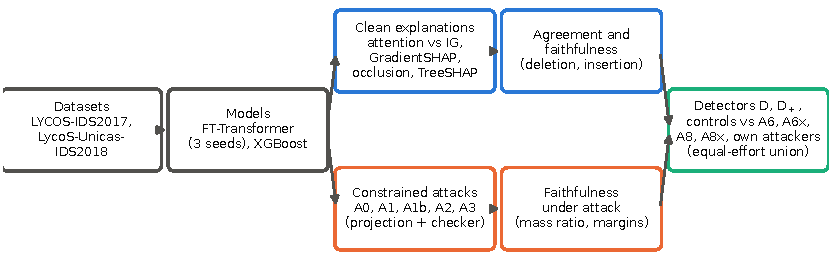
\includegraphics[width=\textwidth]{f_pipeline}
  \caption{Pipeline of the study.}
  \label{f_pipeline}
\end{figure*}

\subsection{Threat model}
\label{sec:threat}
The defender runs a flow classifier, an FT-Transformer, and a learned attack detector on top of it.
The attacker holds a malicious flow and wants the classifier to predict it as benign while the detector stays below its
threshold.
The attacker knows the weights of the classifier and of the detector (white box) and can change only the flow features
that a sender controls, within a per-feature budget and under the protocol relations of the constraint model below.
We consider three levels of attacker knowledge about the detector: none (the attacker ignores the detector), a
differentiable approximation of its scores (stand-ins), and its exact score, with surrogate gradients only where the
exact gradient is zero almost everywhere.
Following the adaptive-attack principle \cite{tramer2020,carlini2017}, a detector is judged by the attacker that models
it, and two detectors are compared at equal attacker effort.
Packet-level attacks, black-box attackers and attacks on the training data are out of scope.

\subsection{Constraint model and validity checker}
\label{sec:constraints}
Of the \nFeatures{} features, \nControls{} are controls the attacker may change within a budget, \nDerived{} are
derived and recomputed from the controls, and \nImmutable{} are immutable (Table~\ref{t_constraints}).
The budget of a control is $\epsilon$ times its clean value, or $\epsilon$ times the training median of its non-zero
values when the clean value is zero.
Class families whose mechanism is the timing and packet count (slow DoS, port scan) have those controls frozen.
A separate validity checker, written as NumPy code apart from the derivation and projection that the attacks use,
re-derived every relation from the written specification and accepted every constrained adversarial row of every
reported attack and detector experiment (Table~\ref{t_constraints}; for the adaptive attacks added in this version,
\sbInvalid{} invalid of \sbRows{} rows on the controls, \axInvalid{} of \axRows{} for A8x and \sxInvalid{} of
\sxRowsWritten{} for A6x).
It shares the specification file and a few helpers with the attack code, so it shows internal consistency rather than
realisability.

% Generated by paper/make_tables_v2.py on 2026-10-30. Do not edit.
% Source: results/stage4_constraints.csv
% Source: results/stage7/stage7d/stage7d_frozen_share.csv
% Source: results/stage7/stage7d/stage7d_frozen_share_2017.csv
\begin{table}[t]
\centering
\footnotesize
\caption{Constraint model of the constrained attacks.}
\label{t_constraints}
\begin{tabular}{lc}
\toprule
Feature role & Count \\
\midrule
Features in the model & $72$ \\
Controls (attacker-perturbed, budgeted) & $18$ \\
\quad of which add-only & $9$ \\
\quad of which either direction & $9$ \\
\quad of which integer & $15$ \\
Derived (recomputed from controls) & $16$ \\
Immutable & $38$ \\
\midrule
\multicolumn{2}{l}{\textit{Class-family freezes (controls frozen because they are the attack mechanism)}} \\
slow dos (2017: DoS Slowhttptest, DoS Slowloris; 2018: DoS Slowloris) & $10$ \\
scan (2017: PortScan; 2018: none) & $10$ \\
\bottomrule
\end{tabular}
\par\smallskip\parbox{\linewidth}{\scriptsize Budget per control and row: $\epsilon$ times the clean value, or $\epsilon$ times the training median of the non-zero values when the clean value is 0 (training split of each dataset). A separate checker validates every adversarial row: 0 invalid of 336{,}093 saved constrained adversarial row records (both datasets, all reported attack and defender experiments; the defender experiments reuse the A1 rows of the attack experiments).}
\end{table}


\subsection{Explanations and faithfulness}
For each FT-Transformer we computed three attention variants over the \nFeatures{} feature tokens: the [CLS] row of the
last layer averaged over heads, the [CLS] row averaged over layers and heads, and attention rollout
\cite{abnar2020}.
A single attention head selected on validation data served as a diagnostic (Appendix~\ref{sec:appendix}).
As references we used IG with the training mean as baseline, GradientSHAP, leave-one-feature-out occlusion, TreeSHAP of
an XGBoost model, the absolute standardised input $|x|$, and a random ranking.
Signed attributions were ranked by their absolute value.

Agreement between two explanations is the Spearman correlation of their feature rankings per row.
Faithfulness was measured by masking features in ranking order with the training mean and recording the probability of
the explained class: the area under the deletion curve (lower is more faithful) and under the insertion curve (higher
is more faithful) \cite{petsiuk2018,samek2017}.
On adversarial rows we used the logit margin of the original class and the gap between most- and least-relevant-first
removal (AOPC gap, where AOPC is the area over the perturbation curve) \cite{samek2017}, and subtracted the change measured under the random control
A0 at the same budget.
Static rankings use the training-set class mean of an explanation, the same vector for every row of a class.
All values are macro averages over classes and means over seeds.

\subsection{Attacks}
\label{sec:attacks}
\paragraph{Non-adaptive attacks.}
Attacks perturbed the controls of the raw flow within their budgets, recomputed derived features, and projected every
iterate back onto the constraint set; they used sign-gradient PGD with \paramSteps{} steps and one random restart.
A0 draws one random point in the same box (random control).
A1 maximises the benign logit margin (evasion).
A1b targets another attack class.
A2 keeps the prediction and minimises the share of rollout attention on the clean top-\paramTopK{} IG features.
A3 combines A1 with the A2 term, with weights $\lambda \in \{100, 1000\}$ and a variant with normalised gradients.
The budget $\epsilon$ ranged from $0.05$ to $2$; headline values use $\epsilon = \paramEpsHead$.
An unconstrained reference applied the same objectives in standardised space with an $L_\infty$ bound and no
constraints; its rows are not valid flows and serve only as a reference.

\paragraph{Adaptive attacks.}
Every adaptive attacker maximises the benign margin, capped at $\kappa = \paramKappa$, minus a hinge on the detector
logit, with $\lambda \in \{1, 100\}$ and a normalised-gradient variant with weight \paramNormW{} (three settings), and
keeps the best projected iterate per row.
A6 attacks D, whose four scores are differentiable, so its objective is the exact score of D; its best iterate is the
one that is flipped and below the threshold under this exact score, and among those the one with the highest
objective.
A8 attacks D$_+$ and replaces each consistency score by a differentiable stand-in: soft-rank Spearman correlation, a
soft top-\paramTopK{} Jaccard overlap, exact cosine similarity, and IG with \paramIGLoss{} steps inside the loss.
A8x attacks D$_+$ with its exact score wherever an exact gradient exists: attention, the four scores of D and the
cosine scores are computed exactly, and IG inside the loss uses \axIGSteps{} Gauss-Legendre steps, as in the true
scores.
Only the \nRankScores{} rank-based scores (Spearman and top-\paramTopK{} Jaccard) keep a surrogate gradient, soft
ranks whose temperature is annealed geometrically from \axTauStart{} to \axTauEnd{} over the steps, because their exact
gradient is zero almost everywhere.
At every step A8x evaluates the true D$_+$ score and keeps, per row, the iterate that is flipped to benign with the
lowest true score, counting it as undetected only if it lies more than \axMargin{} below the threshold.
A6x is A6 with the selection rule of A8x: the same objective, settings, seeds and restart noise, with the iterate kept
by the true D score and the same margin.
A6x was added to test whether the different selection rules of A6 and A8x, rather than the consistency scores, explain
the comparison between D and D$_+$.
Detection was always evaluated with the true scores.
The labels follow the numbering used in the code; A4, A5 and A7 are earlier attack variants that are not part of the
reported analysis (A7 was superseded by A8).

\paragraph{Attackers of the controls.}
Each control detector (Section~\ref{sec:detectors}) was attacked with the same three settings by an attacker that
models its own scores.
The attackers of c0, c1 and c2 use exact gradients, because their scores are differentiable.
The attackers of a1 and a2 use the stand-ins of A8 for their \nConsistency{} consistency scores; for a1 the partner
attention is computed on the clean source rows and held fixed, and for a2 each source row has one fixed draw from the
clean benign bank, so that the attacker and the evaluation use the same feature.
These attackers keep the selection rule of A6.
Control b was not attacked adaptively: its attack run exceeded the memory of the graphics card and was stopped before
any row was written (Section~\ref{sec:limitations}).

\subsection{Detectors and controls}
\label{sec:detectors}
Detector D is a standardised, class-balanced logistic regression on four scores: maximum softmax probability, logit
margin, Mahalanobis distance and mean distance to the \paramKnn{} nearest benign training rows.
Detector D$_+$ adds \nConsistency{} consistency scores between attention (rollout, layer mean) and attribution (gradient
times input, IG with \paramIGDet{} steps), each measured by Spearman correlation, top-\paramTopK{} Jaccard overlap and
cosine similarity, each oriented in the direction validated on validation data; the logistic regression of D$_+$ is
L2-regularised.
Both detectors were trained only on validation data: \paramNegTrain{} benign validation rows predicted benign as
negatives and A1 rows generated on validation source rows as positives; the threshold was set at \paramFPR{} FPR on
\paramNegHeld{} held-out benign validation rows.
Test negatives were \paramNegTest{} genuine benign test rows per seed.

To test whether a difference between D and D$_+$ depends on attention, we trained \nControlsAll{} control detectors on
the same training rows, with the same threshold at \paramFPR{} FPR on the same held-out rows and the inverse
regularisation strength of D$_+$ (\apCplus) for every control; D was not changed.
Each control keeps the four scores of D and replaces the \nConsistency{} consistency scores of D$_+$.
In a1, each row receives the rollout and layer-mean attention of another row of the same true class in the same row set
(a random cyclic shift, so that no row keeps its own attention), and the consistency scores are computed with its own
attribution.
In a2, the attention is drawn at random from clean benign validation rows predicted benign that were used neither for
training nor for the threshold.
In b, attention is replaced by occlusion and GradientSHAP, giving \nConsistency{} attribution-only consistency scores
with the same three measures.
c0 is D with the inverse regularisation strength of D$_+$ and no further score, c1 adds \nConsistency{} features of
standard normal noise, and c2 adds \nConsistency{} statistics of the logits and distances that use no explanation
(Appendix~\ref{sec:appendix}).
For a1 and a2 the draw was repeated with a second shuffle seed, and regenerating the training rows, the scores and the
A6 rows with the original random streams reproduced D, D$_+$ and the A6 rows exactly.
Control a1 uses the true class of each row to choose its partner, so it is a diagnostic control that no deployed
system could compute.

\subsection{Equal-effort evaluation and outcome rules}
\label{sec:protocol}
For each source row we counted an attack as successful and undetected if any candidate aimed at a detector flipped the
prediction to benign and stayed below that detector's threshold: D faced A1 and the three A6 settings, D$_+$ faced A1
and the three A8x settings, and each control faced A1 and the three settings of its own attacker.
The union with A1 and the three A8 settings for D$_+$ is reported for comparison, and the union with A6x for D tests the
selection rule.
This oracle union models an attacker with query access to the detector; equal effort means the same candidates
(restarts, steps and settings) on both sides, not equal computation or equal optimiser quality.
The headline quantity is the difference D$_+$ minus D in the share of such source rows, on the primary row set V1 at
$\epsilon = \paramEpsHead$, per dataset, with a paired bootstrap over source rows within seed (\paramBoot{} draws) and
the three per-seed values; a positive difference means that D$_+$ left more rows undetected.
We also report the paired difference in TPR at the \paramFPR{} FPR threshold on the flipped rows of each attack; for
attacks aimed at D$_+$ this difference is negative by construction and is not used as evidence on its own.

The outcome rules for the comparisons with A8x and with A6x were written down before the code of each attacker, with
the 2017 interval on V1 as the deciding quantity and 2018 reported without changing the conclusion, because D alone
already left few rows undetected there.
For A8x, an interval containing $0$ or lying above $0$ meant that the 2017 gain of D$_+$ measured with A8 did not hold
against A8x; for A6x, an interval above $0$ meant that the comparison does not depend on the selection rule.
Two amendments were recorded before any attack row of the attacker concerned existed: the tolerance of one sanity check
of A8x and the \axMargin{} selection margin, after single-precision noise failed the check at $10^{-5}$, and the chunk
size of A6x, set to that of A6 after a sanity check failed at a smaller chunk (Appendix~\ref{sec:supp},
Table~\ref{t_runs}).

% Experimental setup (Task 42): old Setup without the constraint model (now in Section 3) and without the two
% limitations tables (now Appendix C); T1 and T2 merged into t_data.
\section{Experimental Setup}
\label{sec:setup}

\paragraph{Datasets.}
We used LYCOS-IDS2017 and LycoS-Unicas-IDS2018 (called 2017 and 2018 below), built from the traffic of CIC-IDS2017
and CSE-CIC-IDS2018 \cite{sharafaldin2018,aws_cse_cic_ids2018}, both with the same \nFeatures{} flow features (Table~\ref{t_data}).
On 2017 we removed Heartbleed (\nHeartbleed{} rows) and the structured query language (SQL) injection web attack (\nSqlInjection{} rows, all after
the temporal cut), merged the remaining web attacks, removed feature vectors that carried more than one label and
exact duplicates, and split each (label, day) group in time with gaps between train, validation and test.
On 2018 we removed FTP-Patator (\nFtpRemoved{} rows) and DoS Slowhttptest (\nSlowhttpRemoved{} rows) because the two
classes were indistinguishable in the features, merged the DDoS and web attack variants, removed conflicting and
duplicate vectors, capped large classes, and split at random with stratification, because the file has no timestamps.
This left \nClassesSeventeen{} classes on 2017 and \nClassesEighteen{} on 2018; all cross-dataset comparisons use the
\nCommonClasses{} common attack classes.

% Generated by paper_v3/gen/make_tables_v3.py on 2026-10-30. Do not edit.
% Source: results/stage1_class_counts.csv
% Source: results/stage1_cleaning_report.csv
% Source: results/stage7/stage7b_counts_by_step.csv
% Source: results/stage2_per_class_f1.csv
% Source: results/stage7/stage7b_per_class.csv
\begin{table}[t]
\centering
\footnotesize
\caption{Datasets after cleaning (rows per class and split) and test macro-F1 of the models.}
\label{t_data}
\sbox0{%
\begin{tabular}{lrrrrrr}
\toprule
 & \multicolumn{3}{c}{LYCOS-IDS2017} & \multicolumn{3}{c}{LycoS-Unicas-IDS2018} \\
Class & Train & Val & Test & Train & Val & Test \\
\midrule
Benign & 740{,}728 & 246{,}910 & 246{,}908 & 600{,}000 & 200{,}000 & 200{,}000 \\
Bot & 431 & 144 & 144 & 57{,}660 & 19{,}220 & 19{,}220 \\
DDoS & 56{,}261 & 18{,}754 & 18{,}754 & 180{,}000 & 60{,}000 & 60{,}000 \\
DoS GoldenEye & 3{,}977 & 1{,}326 & 1{,}326 & 16{,}116 & 5{,}372 & 5{,}373 \\
DoS Hulk & 93{,}476 & 31{,}159 & 31{,}158 & 180{,}000 & 60{,}000 & 60{,}000 \\
DoS Slowhttptest & 2{,}770 & 923 & 923 & removed & removed & removed \\
DoS Slowloris & 3{,}080 & 1{,}027 & 1{,}027 & 5{,}428 & 1{,}809 & 1{,}809 \\
FTP-Patator & 2{,}351 & 784 & 783 & removed & removed & removed \\
PortScan & 981 & 327 & 327 & absent & absent & absent \\
SSH-Patator & 1{,}739 & 580 & 580 & 55{,}571 & 18{,}524 & 18{,}524 \\
Web attack & 1{,}187 & 395 & 397 & 256 & 85 & 85 \\
\midrule
Total & 906{,}981 & 302{,}329 & 302{,}327 & 1{,}095{,}031 & 365{,}010 & 365{,}011 \\
\midrule
\multicolumn{7}{l}{\textit{Test macro-F1}} \\
FT-Transformer & \multicolumn{3}{c}{$0.9231$ {\scriptsize ($0.9133$ to $0.9309$)}} & \multicolumn{3}{c}{$0.9924$ {\scriptsize ($0.9915$ to $0.9936$)}} \\
XGBoost & \multicolumn{3}{c}{$0.9515$} & \multicolumn{3}{c}{$0.9977$} \\
\midrule
\multicolumn{7}{l}{\textit{Removed labels (rows before cleaning) and reason}} \\
\multicolumn{7}{l}{2017: Heartbleed ($11$ rows): too few rows for a train / val / test split} \\
\multicolumn{7}{l}{2017: Web Attack SQL Injection ($12$ rows): all rows fall after the temporal cut (test only)} \\
\multicolumn{7}{l}{2018: FTP-Patator ($190{,}300$ rows): indistinguishable from DoS Slowhttptest in the 72 features} \\
\multicolumn{7}{l}{2018: DoS Slowhttptest ($105{,}550$ rows): indistinguishable from FTP-Patator in the 72 features} \\
\bottomrule
\end{tabular}}%
\ifdim\wd0>\textwidth\resizebox{\textwidth}{!}{\usebox0}\else\usebox0\fi
\par\smallskip\parbox{\linewidth}{\scriptsize 2017: temporal split per (label, day) group with gaps between splits. 2018: stratified random split (the file has no timestamps), with per-class caps applied before the split. Removed or absent classes are not modelled on that dataset. Macro-F1: FT-Transformer mean over 3 seeds (seed range), XGBoost one model; same training recipe on both datasets, no tuning on 2018.}
\end{table}


\paragraph{Models.}
We trained an FT-Transformer with \nSeeds{} seeds and an extreme gradient boosting (XGBoost) reference with one recipe on both datasets, without
tuning on 2018.
Test macro-F1 of the FT-Transformer was \fOneFTTSeventeen{} (seed range \fOneFTTSeventeenRange) on 2017 and
\fOneFTTEighteen{} (\fOneFTTEighteenRange) on 2018; XGBoost reached \fOneXGBSeventeen{} and \fOneXGBEighteen{}
(Table~\ref{t_data}).

\paragraph{Explanation and attack sets.}
Clean explanations used up to \paramExplPerClass{} test rows per class that all seeds classified correctly.
Attacks and detectors used the first \paramPerClass{} of these rows per attack class (fewer when a class had fewer;
web attack on 2018 has \nWebTestEighteen{} test rows), the same rows for every seed.

\paragraph{Near-duplicate filter and primary row set.}
For every test row we computed the exact Euclidean distance to its nearest training row in the standardised feature
space of its dataset and flagged rows with a distance below \paramNDThr.
These flags covered \ndSlowlorisSeventeen{} of the DoS Slowloris and \ndWebSeventeen{} of the web attack test rows on
2017, \ndSlowlorisEighteen{} of the DoS Slowloris rows on 2018, and \ndAllSeventeen{} and \ndAllEighteen{} of all test
rows (Appendix~\ref{sec:sens}).
The 2018 attack source rows excluded flagged DoS Slowloris rows by design, while the 2017 attack and detector source
rows were drawn without this filter: on the \nCommonClasses{} common classes they contained \ndSrcCommonSeventeen{}
flagged rows per seed.
We report three row sets: V0 (all source rows), V1 (flagged source rows removed in both datasets) and V2
(DoS Slowloris and web attack removed in both datasets, \nVtwoClasses{} classes).
V1 is the primary set for all results; V0 and V2 are sensitivity analyses (Section~\ref{sec:rq3} and
Appendix~\ref{sec:sens}).
The filter was applied after the attacks and after detector training, by removing source rows from the saved results;
models, attacks and detector thresholds are unchanged.
V1 was fixed as the primary set after the sensitivity results were seen (Appendix~\ref{sec:sens}), which is why V0 and
V2 are reported as well.
Per seed, V1 contains \nSrcVoneSeventeen{} source rows on 2017 (V0: \nSrcVzeroSeventeen) and \nSrcVoneEighteen{} on
2018, where no source row was flagged.

\paragraph{Seeds and uncertainty.}
All reported analyses used seeds 0, 1 and 2 on both datasets (Appendix~\ref{sec:sens}); a preliminary
detector run with seed 0 alone, used during development, is not reported.
We report means with the range over seeds, and for paired detector comparisons \paramCILevel{} bootstrap intervals
(\paramBoot{} draws): within seed for the equal-effort union, and pooled over seeds for the paired true-positive-rate
(TPR) differences.
Neither interval captures variation between seeds, so we give the per-seed values next to every headline difference.

% Results (Task 42): three RQs; claims table of handoff/37_narrative_v2.md sections 3.3 and 3.7 applied; A6x answers
% the selection question. Every result number is a macro.
\section{Results}
\label{sec:results}

Unless stated otherwise, numbers in this section are V1 values (Section~\ref{sec:setup}) on the \nCommonClasses{}
common classes at $\epsilon = \paramEpsHead$, given as the mean over seeds with the seed range in brackets.
V1 is the primary row set; V0 and V2 are in Section~\ref{sec:rq3} and Appendices~\ref{sec:sens} and~\ref{sec:supp}.

\subsection{RQ1: attention is stable but not faithful}
\label{sec:rq1}
\emph{Answer: rollout attention agreed weakly to moderately with attribution methods and was less faithful than IG and
occlusion on both datasets; it changed little under constrained attacks that targeted it, and after an evasion its
faithfulness fell together with that of the other explanation methods.}

\paragraph{Clean data.}
Rollout attention agreed weakly to moderately with the attribution methods on both datasets: its Spearman correlation
was highest with GradientSHAP (\spRolloutGShapVoneSeventeen{} on 2017, \spRolloutGShapVoneEighteen{} on 2018), about one
third with IG (\spRolloutIGVoneSeventeen{}, range \spRolloutIGVoneSeventeenRange; \spRolloutIGVoneEighteen{}, range
\spRolloutIGVoneEighteenRange), \spRolloutOcclVoneSeventeen{} and \spRolloutOcclVoneEighteen{} with occlusion, and
lowest with TreeSHAP of the XGBoost model (\spRolloutTreeShapVoneSeventeen{} and \spRolloutTreeShapVoneEighteen;
Table~\ref{t_clean}).
Last-layer attention showed almost no agreement (Spearman with IG \spLastIGVoneSeventeen{} and \spLastIGVoneEighteen).
Rollout was more faithful than random and less faithful than IG and occlusion.
Its deletion AUC was \aucDelRolloutVoneSeventeen{} on 2017 and \aucDelRolloutVoneEighteen{} on 2018, against
\aucDelIGVoneSeventeen{} and \aucDelIGVoneEighteen{} for IG, \aucDelOcclVoneSeventeen{} and \aucDelOcclVoneEighteen{}
for occlusion, and \aucDelRandomVoneSeventeen{} and \aucDelRandomVoneEighteen{} for random, and insertion AUC gave the
same picture (Table~\ref{t_clean}).
Among the \nMethods{} methods, rollout ranked \rankDelRolloutSeventeen{} and \rankDelRolloutEighteen{} by deletion AUC,
and the ordering of the methods was similar across the datasets (Spearman correlation between the two orderings
\ordSpDelVone{} for deletion and \ordSpInsVone{} for insertion AUC).
Three smaller 2017 results that did not hold on 2018 and a parameter-randomisation check are in
Appendices~\ref{sec:supp} and~\ref{sec:rand}.

% Generated by paper_v3/gen/make_tables_v3.py on 2026-10-30. Do not edit.
% Source: results/stage8/clean_variants.csv
% Source: results/stage8/clean_variants_ordering.csv
\begin{table}[t]
\centering
\footnotesize
\caption{Clean data (V1, 7 common classes): agreement of attention with attribution methods, and deletion and insertion faithfulness of 8 explanation methods.}
\label{t_clean}
\sbox0{%
\begin{tabular}{lcccc}
\toprule
Quantity & 2017 & 2018 & Rank 2017 & Rank 2018 \\
\midrule
\multicolumn{5}{l}{\textit{Agreement: Spearman correlation between attention and attribution rankings}} \\
Attn. rollout vs IG & $0.349$ {\scriptsize ($0.317$ to $0.373$)} & $0.314$ {\scriptsize ($0.244$ to $0.406$)} &  &  \\
Attn. rollout vs GradientSHAP & $0.470$ {\scriptsize ($0.412$ to $0.505$)} & $0.432$ {\scriptsize ($0.365$ to $0.515$)} &  &  \\
Attn. rollout vs Occlusion & $0.396$ {\scriptsize ($0.351$ to $0.435$)} & $0.358$ {\scriptsize ($0.310$ to $0.429$)} &  &  \\
Attn. rollout vs TreeSHAP (XGB) & $0.231$ {\scriptsize ($0.176$ to $0.269$)} & $0.263$ {\scriptsize ($0.226$ to $0.337$)} &  &  \\
Attn. layer mean vs IG & $0.306$ {\scriptsize ($0.268$ to $0.340$)} & $0.238$ {\scriptsize ($0.190$ to $0.334$)} &  &  \\
Attn. last layer vs IG & $0.033$ {\scriptsize ($-0.013$ to $0.092$)} & $0.015$ {\scriptsize ($-0.015$ to $0.048$)} &  &  \\
\midrule
\multicolumn{5}{l}{\textit{Deletion AUC (train-mean masking; lower is more faithful; rank 1 = lowest)}} \\
Attn. rollout & $0.125$ {\scriptsize ($0.114$ to $0.137$)} & $0.119$ {\scriptsize ($0.084$ to $0.178$)} & $5$ & $4$ \\
Attn. layer mean & $0.145$ {\scriptsize ($0.111$ to $0.191$)} & $0.140$ {\scriptsize ($0.113$ to $0.193$)} & $6$ & $5$ \\
Attn. last layer & $0.241$ {\scriptsize ($0.219$ to $0.272$)} & $0.259$ {\scriptsize ($0.174$ to $0.338$)} & $7$ & $7$ \\
IG & $0.020$ {\scriptsize ($0.015$ to $0.024$)} & $0.031$ {\scriptsize ($0.025$ to $0.039$)} & $1$ & $1$ \\
GradientSHAP & $0.058$ {\scriptsize ($0.054$ to $0.061$)} & $0.053$ {\scriptsize ($0.044$ to $0.065$)} & $3$ & $3$ \\
Occlusion & $0.024$ {\scriptsize ($0.018$ to $0.032$)} & $0.049$ {\scriptsize ($0.032$ to $0.067$)} & $2$ & $2$ \\
$|x|$ & $0.079$ {\scriptsize ($0.074$ to $0.084$)} & $0.149$ {\scriptsize ($0.122$ to $0.173$)} & $4$ & $6$ \\
Random & $0.246$ {\scriptsize ($0.240$ to $0.258$)} & $0.345$ {\scriptsize ($0.323$ to $0.380$)} & $8$ & $8$ \\
\multicolumn{3}{l}{\textit{Spearman of the method ordering, 2017 vs 2018}} & \multicolumn{2}{c}{$0.929$} \\
\midrule
\multicolumn{5}{l}{\textit{Insertion AUC (train-mean masking; higher is more faithful; rank 1 = highest)}} \\
Attn. rollout & $0.501$ {\scriptsize ($0.460$ to $0.577$)} & $0.607$ {\scriptsize ($0.541$ to $0.687$)} & $5$ & $4$ \\
Attn. layer mean & $0.470$ {\scriptsize ($0.420$ to $0.544$)} & $0.506$ {\scriptsize ($0.378$ to $0.578$)} & $6$ & $6$ \\
Attn. last layer & $0.252$ {\scriptsize ($0.207$ to $0.285$)} & $0.374$ {\scriptsize ($0.328$ to $0.442$)} & $7$ & $7$ \\
IG & $0.761$ {\scriptsize ($0.736$ to $0.793$)} & $0.864$ {\scriptsize ($0.837$ to $0.878$)} & $1$ & $1$ \\
GradientSHAP & $0.584$ {\scriptsize ($0.578$ to $0.593$)} & $0.795$ {\scriptsize ($0.770$ to $0.817$)} & $4$ & $3$ \\
Occlusion & $0.717$ {\scriptsize ($0.680$ to $0.778$)} & $0.795$ {\scriptsize ($0.782$ to $0.812$)} & $2$ & $2$ \\
$|x|$ & $0.636$ {\scriptsize ($0.629$ to $0.649$)} & $0.604$ {\scriptsize ($0.560$ to $0.656$)} & $3$ & $5$ \\
Random & $0.246$ {\scriptsize ($0.239$ to $0.257$)} & $0.342$ {\scriptsize ($0.320$ to $0.379$)} & $8$ & $8$ \\
\multicolumn{3}{l}{\textit{Spearman of the method ordering, 2017 vs 2018}} & \multicolumn{2}{c}{$0.929$} \\
\bottomrule
\end{tabular}}%
\ifdim\wd0>\textwidth\resizebox{\textwidth}{!}{\usebox0}\else\usebox0\fi
\par\smallskip\parbox{\linewidth}{\scriptsize Macro over the 7 common attack classes, mean over 3 seeds (seed range in brackets), V1 (explanation rows without a near duplicate in the training set). Ranks: position among the 8 methods from the 7-class means. Agreement of the layer-mean and last-layer attention with the other attributions, and all explanation rows (V0): Appendix~\ref{sec:supp}.}
\end{table}


\paragraph{Attention under constrained attacks.}
Under the constrained attack A2, which kept the prediction and minimised the rollout attention on the clean
top-\paramTopK{} IG features, the attention mass on these features kept \massAtwoVoneSeventeen{}
(\massAtwoVoneSeventeenRange) of its clean value on 2017 and \massAtwoVoneEighteen{} (\massAtwoVoneEighteenRange) on
2018, a mean reduction of \massRedAtwoVoneSeventeen{} and \massRedAtwoVoneEighteen{} (Figure~\ref{f_mass_ratio},
Table~\ref{t_attn_attack}).
Under the random control A0 at the same budget the mass kept \massAzeroVoneSeventeen{} (\massAzeroVoneSeventeenRange)
on 2017 and \massAzeroVoneEighteen{} (\massAzeroVoneEighteenRange) on 2018; no comparison with IG at an equal budget
was run.
The joint attack A3 with $\lambda = 1000$ reached \massAthreeVoneSeventeen{} and \massAthreeVoneEighteen.
The unconstrained reference moved the mass further at a standardised budget of $\epsilon = 0.5$ (\massUncVoneSeventeen{}
and \massUncVoneEighteen, a reduction of \massRedUncVoneSeventeen{} and \massRedUncVoneEighteen), with rows that are not
valid flows and with a budget that is not in the units of the constrained attacks.
Attention was therefore stiff under the feature constraints; this does not show that attention cannot be manipulated.
For context, the evasion attack A1 succeeded on \succAoneVoneSeventeen{} and \succAoneVoneEighteen{} of the source
rows (macro over classes), \aoneMinusAzeroVoneSeventeen{} and \aoneMinusAzeroVoneEighteen{} more than A0 (budgets in
Appendix~\ref{sec:supp}).

\begin{figure*}[t]
  \centering
  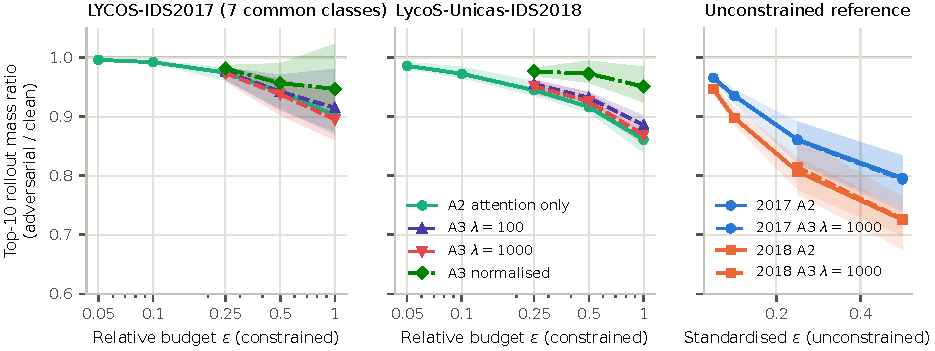
\includegraphics[width=\textwidth]{f_mass_ratio}
  \caption{Top-\paramTopK{} rollout attention mass ratio under A2 and A3, with the unconstrained reference.}
  \label{f_mass_ratio}
\end{figure*}

% Generated by paper_v3/gen/make_tables_v3.py on 2026-10-30. Do not edit.
% Source: results/stage8/sensitivity_stage5.csv
\begin{table}[t]
\centering
\footnotesize
\caption{Attention under protocol-constrained attacks (V1, 7 common classes).}
\label{t_attn_attack}
\begin{tabular}{lcc}
\toprule
Quantity & 2017 & 2018 \\
\midrule
\multicolumn{3}{l}{\textit{Top-10 rollout mass ratio, adversarial / clean (1 = unchanged)}} \\
A2 (attention only), $\epsilon = 0.5$ & $0.946$ {\scriptsize ($0.911$ to $0.967$)} & $0.917$ {\scriptsize ($0.907$ to $0.927$)} \\
A2 (attention only), $\epsilon = 1.0$ & $0.906$ {\scriptsize ($0.864$ to $0.948$)} & $0.861$ {\scriptsize ($0.840$ to $0.874$)} \\
A3 $\lambda{=}1000$ (evasion and attention), $\epsilon = 0.5$ & $0.941$ {\scriptsize ($0.898$ to $0.966$)} & $0.926$ {\scriptsize ($0.917$ to $0.941$)} \\
A3 $\lambda{=}1000$ (evasion and attention), $\epsilon = 1.0$ & $0.900$ {\scriptsize ($0.855$ to $0.947$)} & $0.869$ {\scriptsize ($0.854$ to $0.885$)} \\
A0 (random control), $\epsilon = 1.0$ & $0.994$ {\scriptsize ($0.970$ to $1.025$)} & $0.999$ {\scriptsize ($0.967$ to $1.041$)} \\
A2 unconstrained reference, standardised $\epsilon = 0.5$ & $0.800$ {\scriptsize ($0.748$ to $0.833$)} & $0.726$ {\scriptsize ($0.699$ to $0.743$)} \\
\midrule
\multicolumn{3}{l}{\textit{Evasion success, A1 minus A0}} \\
$\epsilon = 0.5$ & $0.089$ {\scriptsize ($0.002$ to $0.228$)} & $0.082$ {\scriptsize ($-0.004$ to $0.160$)} \\
$\epsilon = 1.0$ & $0.416$ {\scriptsize ($0.216$ to $0.544$)} & $0.416$ {\scriptsize ($0.207$ to $0.550$)} \\
\bottomrule
\end{tabular}
\par\smallskip\parbox{\linewidth}{\scriptsize Macro over the 7 common classes, mean over 3 seeds (seed range). A2 keeps the prediction and minimises the rollout mass on the clean top-10 IG features; A3 also evades. The unconstrained reference has no feature constraints and an $L_\infty$ budget in standardised units, so its budget is not in the units of the constrained attacks. On 2018 no source row is flagged, so V1 equals V0. Other budgets and A3 variants: Appendix~\ref{sec:supp}.}
\end{table}


\paragraph{Faithfulness on flipped rows.}
On rows whose prediction A1 flipped, the margin AOPC gap fell after subtracting the change under A0 for IG, occlusion,
rollout, layer-mean attention, the static class-mean rankings and $|x|$ (Table~\ref{t_flip}).
The change was \flipIGVoneSeventeen{} and \flipIGVoneEighteen{} for IG, \flipOcclVoneSeventeen{} and
\flipOcclVoneEighteen{} for occlusion, \flipRolloutVoneSeventeen{} and \flipRolloutVoneEighteen{} for rollout,
\flipStaticRolloutVoneSeventeen{} and \flipStaticRolloutVoneEighteen{} for the static class-mean rollout, and
\flipAbsXVoneSeventeen{} and \flipAbsXVoneEighteen{} for $|x|$, while the random ranking stayed near zero
(\flipRandomVoneSeventeen{} and \flipRandomVoneEighteen).
The last-layer attention changed with a sign that varied across seeds: \flipLastVoneSeventeen{} on 2017 (seed range
\flipLastVoneSeventeenRange) and \flipLastVoneEighteen{} on 2018 (\flipLastVoneEighteenRange).
On A1 rows that did not flip the change was small for every explainer (IG \notflipIGVoneSeventeen{} and
\notflipIGVoneEighteen), while on rows that the random control A0 flipped to benign by chance (as few as
\nAzeroFlipVoneEighteenMin{} rows in one 2018 seed) the loss was of the same size as on flipped A1 rows on 2017 and
larger on 2018 (IG \azeroflipIGVoneSeventeen{} and \azeroflipIGVoneEighteen).
Because the loss appeared for these explainers on both datasets, including static rankings that the attack cannot
change, was small on rows that did not flip, and appeared also on rows flipped by a random perturbation, it is
consistent with a property of the model at the adversarial point rather than with attack-specific manipulation of
attention; we did not test the mechanism directly.

% Generated by paper_v3/gen/make_tables_v3.py on 2026-10-30. Do not edit.
% Source: results/stage8/flip_split.csv
% Source: results/stage8/flip_split_counts.csv
\begin{table}[t]
\centering
\footnotesize
\setlength{\tabcolsep}{4pt}
\caption{Change of the margin AOPC gap minus the A0 change at $\epsilon = 1$, by row status (V1).}
\label{t_flip}
\sbox0{%
\begin{tabular}{lcccccc}
\toprule
 & \multicolumn{3}{c}{2017} & \multicolumn{3}{c}{2018} \\
Ranking & {\begin{tabular}[t]{@{}c@{}}A1\\flipped\end{tabular}} & {\begin{tabular}[t]{@{}c@{}}A1 not\\flipped\end{tabular}} & {\begin{tabular}[t]{@{}c@{}}A0\\flipped\end{tabular}} & {\begin{tabular}[t]{@{}c@{}}A1\\flipped\end{tabular}} & {\begin{tabular}[t]{@{}c@{}}A1 not\\flipped\end{tabular}} & {\begin{tabular}[t]{@{}c@{}}A0\\flipped\end{tabular}} \\
\midrule
IG & {\begin{tabular}[t]{@{}c@{}}$-11.06$\\{\scriptsize ($-13.04$ to $-9.02$)}\end{tabular}} & {\begin{tabular}[t]{@{}c@{}}$-0.59$\\{\scriptsize ($-2.38$ to $1.17$)}\end{tabular}} & {\begin{tabular}[t]{@{}c@{}}$-11.26$\\{\scriptsize ($-14.08$ to $-7.45$)}\end{tabular}} & {\begin{tabular}[t]{@{}c@{}}$-11.36$\\{\scriptsize ($-12.05$ to $-10.99$)}\end{tabular}} & {\begin{tabular}[t]{@{}c@{}}$-0.46$\\{\scriptsize ($-1.48$ to $0.95$)}\end{tabular}} & {\begin{tabular}[t]{@{}c@{}}$-13.02$\\{\scriptsize ($-14.94$ to $-10.94$)}\end{tabular}} \\
Occlusion & {\begin{tabular}[t]{@{}c@{}}$-12.55$\\{\scriptsize ($-14.26$ to $-10.83$)}\end{tabular}} & {\begin{tabular}[t]{@{}c@{}}$0.43$\\{\scriptsize ($-1.92$ to $3.95$)}\end{tabular}} & {\begin{tabular}[t]{@{}c@{}}$-12.63$\\{\scriptsize ($-15.54$ to $-8.17$)}\end{tabular}} & {\begin{tabular}[t]{@{}c@{}}$-10.61$\\{\scriptsize ($-10.88$ to $-10.25$)}\end{tabular}} & {\begin{tabular}[t]{@{}c@{}}$0.98$\\{\scriptsize ($0.43$ to $1.30$)}\end{tabular}} & {\begin{tabular}[t]{@{}c@{}}$-14.29$\\{\scriptsize ($-16.61$ to $-11.44$)}\end{tabular}} \\
Attn. rollout & {\begin{tabular}[t]{@{}c@{}}$-7.45$\\{\scriptsize ($-8.09$ to $-6.59$)}\end{tabular}} & {\begin{tabular}[t]{@{}c@{}}$0.51$\\{\scriptsize ($-0.58$ to $1.52$)}\end{tabular}} & {\begin{tabular}[t]{@{}c@{}}$-8.35$\\{\scriptsize ($-11.11$ to $-4.49$)}\end{tabular}} & {\begin{tabular}[t]{@{}c@{}}$-7.50$\\{\scriptsize ($-8.93$ to $-5.84$)}\end{tabular}} & {\begin{tabular}[t]{@{}c@{}}$0.27$\\{\scriptsize ($-0.82$ to $1.18$)}\end{tabular}} & {\begin{tabular}[t]{@{}c@{}}$-10.19$\\{\scriptsize ($-13.45$ to $-6.70$)}\end{tabular}} \\
Attn. layer mean & $-7.16$ & $-0.51$ & $-8.95$ & $-7.37$ & $-0.52$ & $-8.30$ \\
Attn. last layer & {\begin{tabular}[t]{@{}c@{}}$1.04$\\{\scriptsize ($-1.33$ to $4.31$)}\end{tabular}} & {\begin{tabular}[t]{@{}c@{}}$0.70$\\{\scriptsize ($-1.94$ to $2.58$)}\end{tabular}} & {\begin{tabular}[t]{@{}c@{}}$0.17$\\{\scriptsize ($-2.54$ to $4.04$)}\end{tabular}} & {\begin{tabular}[t]{@{}c@{}}$-1.16$\\{\scriptsize ($-2.92$ to $0.34$)}\end{tabular}} & {\begin{tabular}[t]{@{}c@{}}$-0.03$\\{\scriptsize ($-0.60$ to $0.84$)}\end{tabular}} & {\begin{tabular}[t]{@{}c@{}}$-1.88$\\{\scriptsize ($-5.26$ to $0.71$)}\end{tabular}} \\
Static rollout (class mean) & $-5.43$ & $0.51$ & $-5.49$ & $-6.19$ & $1.54$ & $-8.41$ \\
Static IG (class mean) & $-9.72$ & $0.33$ & $-9.38$ & $-10.07$ & $0.48$ & $-10.38$ \\
$|x|$ & $-6.60$ & $1.89$ & $-7.00$ & $-5.97$ & $0.87$ & $-7.91$ \\
Random & $0.02$ & $-0.28$ & $-1.19$ & $0.25$ & $-0.30$ & $1.70$ \\
\midrule
Rows per seed & 716, 545, 414 & 185, 356, 487 & 218, 43, 138 & 262, 850, 614 & 723, 135, 371 & 20, 208, 43 \\
\bottomrule
\end{tabular}}%
\ifdim\wd0>\textwidth\resizebox{\textwidth}{!}{\usebox0}\else\usebox0\fi
\par\smallskip\parbox{\linewidth}{\scriptsize Change of the margin AOPC gap from the clean to the adversarial row, minus the mean change over all A0 rows at the same budget; train-mean masking; macro over classes, mean over seeds (seed range for IG, occlusion, rollout and last-layer attention). More negative = larger loss of faithfulness. A0 flipped: rows that the random control flipped to benign by chance. 2017: 7 common classes.}
\end{table}


\subsection{RQ2: consistency monitoring against adaptive attackers}
\label{sec:rq2}
\emph{Answer: the consistency scores helped against an attacker that ignored them, largely without attention, but not
against attackers that optimised the detector's exact score; against those, D$_+$ left more attack rows successful and
undetected than D on both datasets, and the gain measured with a stand-in attacker did not hold.}

\paragraph{Detectors and the non-adaptive attacker.}
Both detectors separated validation positives well (validation AUROC of D \valAurocDSeventeenRange{} on 2017 and
\valAurocDEighteenRange{} on 2018 over seeds, D$_+$ \valAurocDplusSeventeenRange{} and \valAurocDplusEighteenRange;
realised test FPR of D \testFprDSeventeenRange{} and \testFprDEighteenRange).
The validation AUROC is measured on the flipped validation positives that were also used to fit the detectors, so it
is in-sample; the realised test FPR is the out-of-sample figure.
Against A6, which ignores the consistency scores, D$_+$ detected more of the evading rows than D: the paired TPR
difference D$_+$ minus D on A6 rows ($\lambda = 1$) was \tprAsixOneVoneSeventeen{} (\tprAsixOneVoneSeventeenCI) on 2017
and \tprAsixOneVoneEighteen{} (\tprAsixOneVoneEighteenCI) on 2018 (Table~\ref{t_attacks}).

% Generated by paper_v3/gen/make_tables_v3.py on 2026-10-30. Do not edit.
% Source: results/stage8/sensitivity_defenders.csv
% Source: results/stage8/sensitivity_paired.csv
% Source: results/stage9/a8x/summary_tpr.csv
% Source: results/stage9/a8x/summary_extra.csv
\begin{table}[t]
\centering
\footnotesize
\setlength{\tabcolsep}{4pt}
\caption{Success and undetected share per attack at $\epsilon = 1$ (V1, 7 common classes), and the paired TPR difference D$_+$ minus D on the flipped rows of each attack.}
\label{t_attacks}
\textit{2017}\par\smallskip
\sbox0{%
\begin{tabular}{lllcccc}
\toprule
Attack & Aimed at & Attacker & Success & Undet. D & Undet. D$_+$ & TPR D$_+$ minus D [95\% CI] \\
\midrule
A1 & none &  & $0.620$ {\scriptsize ($0.459$ to $0.795$)} & $0.016$ {\scriptsize ($0.000$ to $0.046$)} & $0.001$ {\scriptsize ($0.000$ to $0.003$)} & $+0.023$ {\scriptsize [$+0.016$, $+0.031$]} \\
A6 $\lambda{=}1$ & D & exact & $0.496$ {\scriptsize ($0.275$ to $0.714$)} & $0.204$ {\scriptsize ($0.148$ to $0.272$)} & $0.086$ {\scriptsize ($0.009$ to $0.210$)} & $+0.238$ {\scriptsize [$+0.213$, $+0.265$]} \\
A6 $\lambda{=}100$ & D & exact & $0.319$ {\scriptsize ($0.108$ to $0.489$)} & $0.127$ {\scriptsize ($0.007$ to $0.234$)} & $0.052$ {\scriptsize ($0.001$ to $0.132$)} & $+0.234$ {\scriptsize [$+0.199$, $+0.271$]} \\
A6 norm. & D & exact & $0.613$ {\scriptsize ($0.535$ to $0.735$)} & $0.181$ {\scriptsize ($0.098$ to $0.307$)} & $0.055$ {\scriptsize ($0.006$ to $0.135$)} & $+0.204$ {\scriptsize [$+0.185$, $+0.223$]} \\
A8 $\lambda{=}1$ & D$_+$ & stand-in & $0.524$ {\scriptsize ($0.332$ to $0.740$)} & $0.162$ {\scriptsize ($0.134$ to $0.191$)} & $0.141$ {\scriptsize ($0.064$ to $0.277$)} & $+0.040$ {\scriptsize [$+0.013$, $+0.066$]} \\
A8 $\lambda{=}100$ & D$_+$ & stand-in & $0.427$ {\scriptsize ($0.213$ to $0.637$)} & $0.117$ {\scriptsize ($0.024$ to $0.178$)} & $0.125$ {\scriptsize ($0.012$ to $0.279$)} & $-0.017$ {\scriptsize [$-0.049$, $+0.013$]} \\
A8 norm. & D$_+$ & stand-in & $0.620$ {\scriptsize ($0.508$ to $0.776$)} & $0.120$ {\scriptsize ($0.069$ to $0.182$)} & $0.112$ {\scriptsize ($0.037$ to $0.262$)} & $+0.013$ {\scriptsize [$-0.010$, $+0.034$]} \\
A8x $\lambda{=}1$ & D$_+$ & exact obj. & $0.519$ {\scriptsize ($0.307$ to $0.747$)} & $0.191$ {\scriptsize ($0.125$ to $0.294$)} & $0.282$ {\scriptsize ($0.097$ to $0.436$)} & $-0.175$ {\scriptsize [$-0.203$, $-0.148$]} \\
A8x $\lambda{=}100$ & D$_+$ & exact obj. & $0.438$ {\scriptsize ($0.253$ to $0.640$)} & $0.162$ {\scriptsize ($0.038$ to $0.320$)} & $0.242$ {\scriptsize ($0.020$ to $0.438$)} & $-0.182$ {\scriptsize [$-0.210$, $-0.154$]} \\
A8x norm. & D$_+$ & exact obj. & $0.621$ {\scriptsize ($0.497$ to $0.774$)} & $0.175$ {\scriptsize ($0.081$ to $0.287$)} & $0.252$ {\scriptsize ($0.051$ to $0.477$)} & $-0.124$ {\scriptsize [$-0.150$, $-0.097$]} \\
\bottomrule
\end{tabular}}%
\ifdim\wd0>\textwidth\resizebox{\textwidth}{!}{\usebox0}\else\usebox0\fi
\par\medskip
\textit{2018}\par\smallskip
\sbox0{%
\begin{tabular}{lllcccc}
\toprule
Attack & Aimed at & Attacker & Success & Undet. D & Undet. D$_+$ & TPR D$_+$ minus D [95\% CI] \\
\midrule
A1 & none &  & $0.584$ {\scriptsize ($0.266$ to $0.863$)} & $0.001$ {\scriptsize ($0.000$ to $0.001$)} & $0.000$ {\scriptsize ($0.000$ to $0.001$)} & $+0.001$ {\scriptsize [$-0.001$, $+0.002$]} \\
A6 $\lambda{=}1$ & D & exact & $0.303$ {\scriptsize ($0.129$ to $0.504$)} & $0.014$ {\scriptsize ($0.002$ to $0.036$)} & $0.002$ {\scriptsize ($0.000$ to $0.007$)} & $+0.037$ {\scriptsize [$+0.021$, $+0.051$]} \\
A6 $\lambda{=}100$ & D & exact & $0.280$ {\scriptsize ($0.092$ to $0.481$)} & $0.006$ {\scriptsize ($0.001$ to $0.014$)} & $0.003$ {\scriptsize ($0.000$ to $0.008$)} & $+0.013$ {\scriptsize [$+0.001$, $+0.025$]} \\
A6 norm. & D & exact & $0.493$ {\scriptsize ($0.281$ to $0.722$)} & $0.013$ {\scriptsize ($0.001$ to $0.025$)} & $0.000$ {\scriptsize ($0.000$ to $0.001$)} & $+0.025$ {\scriptsize [$+0.018$, $+0.033$]} \\
A8 $\lambda{=}1$ & D$_+$ & stand-in & $0.335$ {\scriptsize ($0.123$ to $0.602$)} & $0.007$ {\scriptsize ($0.001$ to $0.016$)} & $0.013$ {\scriptsize ($0.001$ to $0.020$)} & $-0.017$ {\scriptsize [$-0.032$, $-0.003$]} \\
A8 $\lambda{=}100$ & D$_+$ & stand-in & $0.324$ {\scriptsize ($0.131$ to $0.552$)} & $0.007$ {\scriptsize ($0.000$ to $0.019$)} & $0.013$ {\scriptsize ($0.001$ to $0.018$)} & $-0.016$ {\scriptsize [$-0.031$, $+0.001$]} \\
A8 norm. & D$_+$ & stand-in & $0.504$ {\scriptsize ($0.237$ to $0.748$)} & $0.000$ {\scriptsize ($0.000$ to $0.001$)} & $0.006$ {\scriptsize ($0.000$ to $0.011$)} & $-0.012$ {\scriptsize [$-0.018$, $-0.006$]} \\
A8x $\lambda{=}1$ & D$_+$ & exact obj. & $0.336$ {\scriptsize ($0.136$ to $0.572$)} & $0.009$ {\scriptsize ($0.000$ to $0.021$)} & $0.021$ {\scriptsize ($0.001$ to $0.045$)} & $-0.037$ {\scriptsize [$-0.055$, $-0.019$]} \\
A8x $\lambda{=}100$ & D$_+$ & exact obj. & $0.317$ {\scriptsize ($0.124$ to $0.522$)} & $0.008$ {\scriptsize ($0.000$ to $0.021$)} & $0.019$ {\scriptsize ($0.000$ to $0.045$)} & $-0.032$ {\scriptsize [$-0.050$, $-0.015$]} \\
A8x norm. & D$_+$ & exact obj. & $0.515$ {\scriptsize ($0.268$ to $0.734$)} & $0.012$ {\scriptsize ($0.000$ to $0.021$)} & $0.016$ {\scriptsize ($0.000$ to $0.027$)} & $-0.009$ {\scriptsize [$-0.021$, $+0.003$]} \\
\bottomrule
\end{tabular}}%
\ifdim\wd0>\textwidth\resizebox{\textwidth}{!}{\usebox0}\else\usebox0\fi
\par\smallskip\parbox{\linewidth}{\scriptsize Success: share of source rows predicted benign; Undet.: also below the detector threshold at 5\% FPR on validation benign rows. Mean over seeds pooled over rows (seed range). TPR difference: paired bootstrap over the flipped rows (1,000 draws). Attacker: exact, the attacker's objective is the exact detector score; stand-in, differentiable stand-ins for the consistency scores; exact obj., the exact score with surrogate gradients for the eight rank-based scores. The rows of an attack aimed at D$_+$ were optimised against D$_+$, so a negative TPR difference on them is expected by construction; the equal-effort comparison is Table~\ref{t_union_adaptive}.}
\end{table}


The controls (Section~\ref{sec:detectors}, Table~\ref{t_dplus_ablation}) show that this gain against A6 is largely
obtained without attention: the TPR difference to D was \ablBMinusDSeventeen{} and \ablBMinusDEighteen{} for the
attribution-only control b and \ablCtwoMinusDSeventeen{} and \ablCtwoMinusDEighteen{} for c2 with logit and distance
statistics, while c0 (\ablCzeroMinusDSeventeen) and c1 (\ablConeMinusDSeventeen) show that the regulariser and the
number of scores do not explain it.
Shuffled attention from another row of the same class (a1) kept most of the gain on 2017 and all of it on 2018
(\ablAoneMinusDSeventeen{} and \ablAoneMinusDEighteen), attention from clean benign rows (a2) kept
\ablAtwoMinusDSeventeen{} and \ablAtwoMinusDEighteen, and the pairing of a row's own attention with its attribution,
D$_+$ minus a1 against A6, added \ablPairSeventeen{} (\ablPairSeventeenCI) on 2017 and nothing detectable on 2018
(\ablPairEighteen, \ablPairEighteenCI).

% Generated by paper/make_tables_v2.py on 2026-10-30. Do not edit.
% Source: results/stage9/ablation/summary_detection.csv
% Source: results/stage9/ablation/summary_paired.csv
% Source: results/stage9/ablation/summary_defenders.csv
\begin{table}[t]
\centering
\footnotesize
\caption{Controls for D$_+$: detection of A1 and A6 rows by D, D$_+$ and the six controls (V1, $\epsilon = 1$).}
\label{t_dplus_ablation}
\textit{2017 (1{,}675 A1 rows, 1{,}341 A6 $\lambda{=}1$ rows)}\par\smallskip
\sbox0{%
\begin{tabular}{lcccccccc}
\toprule
Quantity & D & D$_+$ & a1 & a2 & b & c0 & c1 & c2 \\
\midrule
TPR on A1 & $0.975$ & $0.998$ & $0.996$ & $0.980$ & $0.998$ & $0.975$ & $0.976$ & $0.994$ \\
TPR on A6 $\lambda{=}1$ & $0.589$ & $0.827$ & $0.782$ & $0.688$ & $0.855$ & $0.589$ & $0.547$ & $0.782$ \\
A6 $\lambda{=}1$ minus D &  & {\begin{tabular}[t]{@{}c@{}}$0.238$\\{\scriptsize [$0.214$, $0.265$]}\end{tabular}} & {\begin{tabular}[t]{@{}c@{}}$0.192$\\{\scriptsize [$0.166$, $0.217$]}\end{tabular}} & {\begin{tabular}[t]{@{}c@{}}$0.099$\\{\scriptsize [$0.075$, $0.125$]}\end{tabular}} & {\begin{tabular}[t]{@{}c@{}}$0.265$\\{\scriptsize [$0.238$, $0.294$]}\end{tabular}} & {\begin{tabular}[t]{@{}c@{}}$0.000$\\{\scriptsize [$0.000$, $0.000$]}\end{tabular}} & {\begin{tabular}[t]{@{}c@{}}$-0.043$\\{\scriptsize [$-0.055$, $-0.029$]}\end{tabular}} & {\begin{tabular}[t]{@{}c@{}}$0.193$\\{\scriptsize [$0.172$, $0.216$]}\end{tabular}} \\
D$_+$ minus control &  &  & {\begin{tabular}[t]{@{}c@{}}$0.045$\\{\scriptsize [$0.028$, $0.065$]}\end{tabular}} & {\begin{tabular}[t]{@{}c@{}}$0.139$\\{\scriptsize [$0.113$, $0.166$]}\end{tabular}} & {\begin{tabular}[t]{@{}c@{}}$-0.028$\\{\scriptsize [$-0.050$, $-0.002$]}\end{tabular}} & {\begin{tabular}[t]{@{}c@{}}$0.238$\\{\scriptsize [$0.212$, $0.264$]}\end{tabular}} & {\begin{tabular}[t]{@{}c@{}}$0.280$\\{\scriptsize [$0.254$, $0.305$]}\end{tabular}} & {\begin{tabular}[t]{@{}c@{}}$0.045$\\{\scriptsize [$0.015$, $0.075$]}\end{tabular}} \\
Realised test FPR & $0.052$ & $0.053$ & $0.060$ & $0.057$ & $0.056$ & $0.052$ & $0.053$ & $0.050$ \\
\bottomrule
\end{tabular}}%
\ifdim\wd0>\textwidth\resizebox{\textwidth}{!}{\usebox0}\else\usebox0\fi
\par\medskip
\textit{2018 (1{,}726 A1 rows, 896 A6 $\lambda{=}1$ rows)}\par\smallskip
\sbox0{%
\begin{tabular}{lcccccccc}
\toprule
Quantity & D & D$_+$ & a1 & a2 & b & c0 & c1 & c2 \\
\midrule
TPR on A1 & $0.999$ & $0.999$ & $0.998$ & $0.999$ & $1.000$ & $0.999$ & $0.998$ & $1.000$ \\
TPR on A6 $\lambda{=}1$ & $0.955$ & $0.992$ & $0.991$ & $0.975$ & $0.997$ & $0.960$ & $0.954$ & $0.993$ \\
A6 $\lambda{=}1$ minus D &  & {\begin{tabular}[t]{@{}c@{}}$0.037$\\{\scriptsize [$0.022$, $0.051$]}\end{tabular}} & {\begin{tabular}[t]{@{}c@{}}$0.036$\\{\scriptsize [$0.023$, $0.049$]}\end{tabular}} & {\begin{tabular}[t]{@{}c@{}}$0.020$\\{\scriptsize [$0.010$, $0.030$]}\end{tabular}} & {\begin{tabular}[t]{@{}c@{}}$0.041$\\{\scriptsize [$0.028$, $0.055$]}\end{tabular}} & {\begin{tabular}[t]{@{}c@{}}$0.004$\\{\scriptsize [$0.001$, $0.009$]}\end{tabular}} & {\begin{tabular}[t]{@{}c@{}}$-0.001$\\{\scriptsize [$-0.008$, $0.006$]}\end{tabular}} & {\begin{tabular}[t]{@{}c@{}}$0.038$\\{\scriptsize [$0.025$, $0.052$]}\end{tabular}} \\
D$_+$ minus control &  &  & {\begin{tabular}[t]{@{}c@{}}$0.001$\\{\scriptsize [$-0.007$, $0.010$]}\end{tabular}} & {\begin{tabular}[t]{@{}c@{}}$0.017$\\{\scriptsize [$0.006$, $0.028$]}\end{tabular}} & {\begin{tabular}[t]{@{}c@{}}$-0.004$\\{\scriptsize [$-0.012$, $0.002$]}\end{tabular}} & {\begin{tabular}[t]{@{}c@{}}$0.032$\\{\scriptsize [$0.019$, $0.047$]}\end{tabular}} & {\begin{tabular}[t]{@{}c@{}}$0.038$\\{\scriptsize [$0.023$, $0.055$]}\end{tabular}} & {\begin{tabular}[t]{@{}c@{}}$-0.001$\\{\scriptsize [$-0.009$, $0.008$]}\end{tabular}} \\
Realised test FPR & $0.055$ & $0.049$ & $0.055$ & $0.058$ & $0.048$ & $0.055$ & $0.052$ & $0.055$ \\
\bottomrule
\end{tabular}}%
\ifdim\wd0>\textwidth\resizebox{\textwidth}{!}{\usebox0}\else\usebox0\fi
\par\smallskip\parbox{\linewidth}{\scriptsize Controls (Section~\ref{sec:methods}): a1, attention of another row of the same true class; a2, attention of clean benign validation rows; b, occlusion and GradientSHAP instead of attention; c0, D with the regularisation of D$_+$; c1, D with 12 noise features; c2, D with 12 logit and distance statistics. Thresholds at 5\% FPR on validation benign rows. TPR on the source rows that the attack flipped to benign, pooled over seeds 0 to 2; differences are paired TPR differences with a 95\% paired bootstrap interval (1,000 draws over the flipped rows pooled over seeds, threshold-centred per seed), computed separately from the intervals in Section~\ref{sec:sens}, so the interval of D$_+$ minus D can differ from them in the last digit. Realised test FPR: mean over seeds on the benign test negatives.}
\end{table}


\paragraph{Attackers that model the consistency scores.}
Against A8, which models the consistency scores through stand-ins, the gain largely disappeared: the paired TPR
difference on A8 rows ($\lambda = 1$) was \tprAeightOneVoneSeventeen{} (\tprAeightOneVoneSeventeenCI) on 2017 and
\tprAeightOneVoneEighteen{} (\tprAeightOneVoneEighteenCI) on 2018.
Against A8x, which optimises the exact score of D$_+$ (Section~\ref{sec:attacks}), D$_+$ detected fewer of the attack
rows than D: \xtprAxOneVoneSeventeen{} (\xtprAxOneVoneSeventeenCI) on 2017 and \xtprAxOneVoneEighteen{}
(\xtprAxOneVoneEighteenCI) on 2018, and from \xtprAxVoneRangeSeventeen{} over the three settings on 2017
(Table~\ref{t_attacks}).
A8x flipped about as many rows as A8 (success \xsuccAxOneVoneSeventeen{} against \xsuccAeightOneVoneSeventeen{} on 2017)
but left more of them undetected by D$_+$ (\xundetAxOneVoneSeventeen{} against \xundetAeightOneVoneSeventeen).
These rows were optimised against D$_+$, so this comparison alone is not evidence; the equal-effort union is.

\paragraph{Equal-effort comparison.}
Under equal attacker effort (Table~\ref{t_union_adaptive}, Figure~\ref{f_headline}), with D facing A1 and A6 and D$_+$
facing A1 and A8x, D$_+$ left more source rows successful and undetected than D: \axHeadVoneSeventeenDplus{} against
\axHeadVoneSeventeenD{} on 2017, a difference of \axHeadVoneSeventeen{} (\paramCILevel{} CI \axHeadVoneSeventeenCI),
and \axHeadVoneEighteenDplus{} against \axHeadVoneEighteenD{} on 2018, a difference of \axHeadVoneEighteen{}
(\axHeadVoneEighteenCI).
With A8 instead of A8x the 2017 difference had been \axStandinVoneSeventeen{} (\axStandinVoneSeventeenCI), and on 2018
\axStandinVoneEighteen{} (\axStandinVoneEighteenCI).
Per seed, the 2017 differences were \axHeadVoneSeventeenSeeds{} and the 2018 differences \axHeadVoneEighteenSeeds{}
(seeds 0, 1 and 2); \axHeadOppSeedsSeventeen{} seed on 2017 and \axHeadOppSeedsEighteen{} on 2018 had the opposite
sign.
By the outcome rule recorded before the A8x runs (Section~\ref{sec:protocol}), the 2017 gain of D$_+$ against A8 did
not hold against the exact-objective attacker.

These numbers come with caveats that limit how far they generalise.
They rest on \nSeeds{} seeds, and on each dataset \axHeadOppSeedsSeventeen{} seed (2017) and
\axHeadOppSeedsEighteen{} seed (2018) had the opposite sign; the interval is a bootstrap over source rows within seed
and does not capture variation between seeds.
A8x still uses surrogate gradients for the \nRankScores{} rank-based scores; a better search on these terms could only
find further undetected rows for D$_+$.
The controls a1 and a2 faced stand-in attackers, so their comparison with D$_+$ under A8x is not at equal attacker
strength, and control b was not attacked adaptively because its run exceeded the memory of the graphics card.
On 2018 D alone left only \axHeadVoneEighteenD{} of the source rows undetected, so the 2018 difference sits near a floor
and its lower bound is close to $0$.
Finally, the equal-effort protocol fixes candidates, steps and settings, not optimiser quality: whether A6 is as strong
an attack on D as A8x is on D$_+$ was not measured (see below and Section~\ref{sec:limitations}).

\begin{figure*}[t]
  \centering
  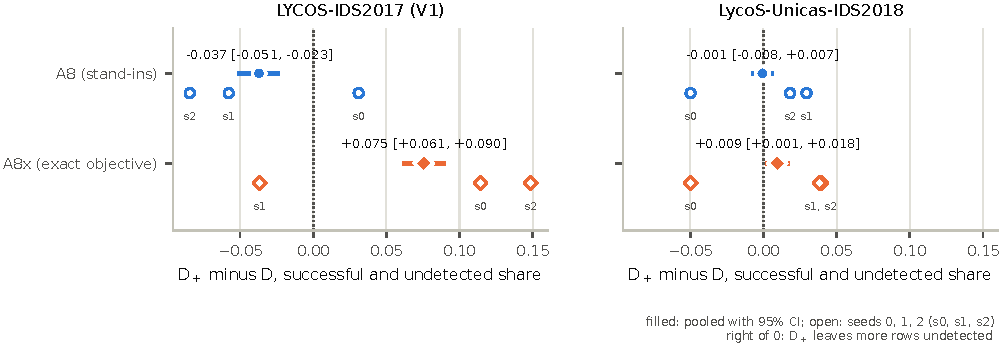
\includegraphics[width=\textwidth]{f_headline}
  \caption{Equal-effort union at $\epsilon = \paramEpsHead$ (V1): D$_+$ minus D in the share of successful and
    undetected source rows when D$_+$ faces the stand-in attacker A8 or the exact-objective attacker A8x (D faces A6 in
    both). Filled marks: pooled difference with the \paramCILevel{} paired bootstrap interval (within seed); open
    marks: seeds 0, 1 and 2.}
  \label{f_headline}
\end{figure*}

% Generated by paper_v3/gen/make_tables_v3.py on 2026-10-30. Do not edit.
% Source: results/stage9/a8x/summary_union.csv
% Source: results/stage9/a6x/summary_union.csv
% Source: results/stage9/adaptive/summary_union.csv
% Source: results/stage9/a8x/summary_extra.csv
% Source: results/stage9/adaptive/{2017,2018}/standin_quality.csv
\begin{table}[t]
\centering
\footnotesize
\setlength{\tabcolsep}{3pt}
\caption{Equal-effort union at $\epsilon = 1$ (V1): share of source rows that are successful and undetected, each detector against its own attackers.}
\label{t_union_adaptive}
\textit{2017, V1 (901 source rows per seed)}\par\smallskip
\sbox0{%
\begin{tabular}{lllcccc}
\toprule
Detector & Attacker & Type & Undet. & Minus D [95\% CI] & Seeds 0 / 1 / 2 & Minus D$_+$ (A8x) [95\% CI] \\
\midrule
D & A1 + A6 $\times 3$ & exact & $0.266$ & (reference) &  & $-0.075$ {\scriptsize [$-0.090$, $-0.061$]} \\
D & A1 + A6x $\times 3$ & exact & $0.266$ & $0.000$ {\scriptsize [$+0.000$, $+0.000$]} & $0.000\,/\,0.000\,/\,0.000$ &  \\
\textbf{D$_+$} & \textbf{A1 + A8x $\times 3$} & exact obj. & $0.341$ & \textbf{$+0.075$ {\scriptsize [$+0.061$, $+0.090$]}} & $+0.114\,/\,-0.037\,/\,+0.149$ & (reference) \\
D$_+$ & A1 + A8 $\times 3$ & stand-in & $0.229$ & $-0.037$ {\scriptsize [$-0.051$, $-0.023$]} & $+0.031\,/\,-0.058\,/\,-0.084$ &  \\
\midrule
c0 & A1 + own $\times 3$ & exact & $0.266$ & $0.000$ {\scriptsize [$-0.007$, $+0.009$]} & $-0.004\,/\,+0.002\,/\,+0.003$ & $-0.075$ {\scriptsize [$-0.089$, $-0.061$]} \\
c1 & A1 + own $\times 3$ & exact & $0.280$ & $+0.014$ {\scriptsize [$+0.004$, $+0.024$]} & $+0.011\,/\,-0.001\,/\,+0.032$ & $-0.061$ {\scriptsize [$-0.075$, $-0.048$]} \\
c2 & A1 + own $\times 3$ & exact & $0.273$ & $+0.008$ {\scriptsize [$-0.006$, $+0.023$]} & $-0.075\,/\,+0.081\,/\,+0.018$ & $-0.068$ {\scriptsize [$-0.083$, $-0.052$]} \\
a1 & A1 + own $\times 3$ & stand-in ($R^2$ $0.983$ / $0.800$) & $0.344$ & $+0.078$ {\scriptsize [$+0.063$, $+0.094$]} & $+0.206\,/\,-0.112\,/\,+0.141$ & $+0.003$ {\scriptsize [$-0.010$, $+0.017$]} \\
a2 & A1 + own $\times 3$ & stand-in ($R^2$ $0.980$ / $0.803$) & $0.278$ & $+0.013$ {\scriptsize [$-0.003$, $+0.029$]} & $-0.031\,/\,-0.032\,/\,+0.101$ & $-0.063$ {\scriptsize [$-0.075$, $-0.050$]} \\
b & \multicolumn{6}{l}{not attacked adaptively (Section~\ref{sec:limitations})} \\
\bottomrule
\end{tabular}}%
\ifdim\wd0>\textwidth\resizebox{\textwidth}{!}{\usebox0}\else\usebox0\fi
\par\medskip
\textit{2018, V1 (985 source rows per seed)}\par\smallskip
\sbox0{%
\begin{tabular}{lllcccc}
\toprule
Detector & Attacker & Type & Undet. & Minus D [95\% CI] & Seeds 0 / 1 / 2 & Minus D$_+$ (A8x) [95\% CI] \\
\midrule
D & A1 + A6 $\times 3$ & exact & $0.023$ & (reference) &  & $-0.009$ {\scriptsize [$-0.018$, $-0.001$]} \\
D & A1 + A6x $\times 3$ & exact & $0.023$ & $0.000$ {\scriptsize [$+0.000$, $+0.000$]} & $0.000\,/\,0.000\,/\,0.000$ &  \\
\textbf{D$_+$} & \textbf{A1 + A8x $\times 3$} & exact obj. & $0.032$ & \textbf{$+0.009$ {\scriptsize [$+0.001$, $+0.018$]}} & $-0.050\,/\,+0.040\,/\,+0.039$ & (reference) \\
D$_+$ & A1 + A8 $\times 3$ & stand-in & $0.022$ & $-0.001$ {\scriptsize [$-0.008$, $+0.007$]} & $-0.050\,/\,+0.029\,/\,+0.018$ &  \\
\midrule
c0 & A1 + own $\times 3$ & exact & $0.015$ & $-0.008$ {\scriptsize [$-0.013$, $-0.004$]} & $-0.009\,/\,0.000\,/\,-0.015$ & $-0.018$ {\scriptsize [$-0.025$, $-0.010$]} \\
c1 & A1 + own $\times 3$ & exact & $0.019$ & $-0.004$ {\scriptsize [$-0.008$, $+0.001$]} & $-0.006\,/\,+0.010\,/\,-0.015$ & $-0.013$ {\scriptsize [$-0.020$, $-0.006$]} \\
c2 & A1 + own $\times 3$ & exact & $0.055$ & $+0.032$ {\scriptsize [$+0.023$, $+0.042$]} & $-0.049\,/\,+0.161\,/\,-0.015$ & $+0.023$ {\scriptsize [$+0.013$, $+0.032$]} \\
a1 & A1 + own $\times 3$ & stand-in ($R^2$ $0.946$ / $0.726$) & $0.006$ & $-0.016$ {\scriptsize [$-0.022$, $-0.011$]} & $-0.040\,/\,+0.006\,/\,-0.015$ & $-0.026$ {\scriptsize [$-0.032$, $-0.019$]} \\
a2 & A1 + own $\times 3$ & stand-in ($R^2$ $0.947$ / $0.736$) & $0.021$ & $-0.001$ {\scriptsize [$-0.007$, $+0.004$]} & $-0.010\,/\,+0.020\,/\,-0.014$ & $-0.011$ {\scriptsize [$-0.018$, $-0.004$]} \\
b & \multicolumn{6}{l}{not attacked adaptively (Section~\ref{sec:limitations})} \\
\bottomrule
\end{tabular}}%
\ifdim\wd0>\textwidth\resizebox{\textwidth}{!}{\usebox0}\else\usebox0\fi
\par\smallskip\parbox{\linewidth}{\scriptsize A source row counts if any candidate aimed at that detector flips it to benign and stays below the detector's threshold (5\% FPR). Minus D: difference to D under A1 + A6 $\times 3$ (for the A6x row: D under A6x minus D under A6); a positive value means more rows evade undetected, which is worse for the defender. Paired bootstrap over source rows within seed, 1,000 draws; the interval does not capture variation between seeds. Type: exact, the attacker optimises the exact score; exact obj., the exact score with surrogate gradients for the eight rank-based consistency scores; stand-in, differentiable stand-ins ($R^2$ median / minimum over features and seeds). Comparisons of a1 or a2 with D$_+$ under A8x are not at equal attacker strength. The D$_+$ row with A8 is shown for comparison only.}
\end{table}


On 2017 the direction held per attack setting (\axLamOneVoneSeventeen, \axLamHundredVoneSeventeen{} and
\axNormVoneSeventeen; Table~\ref{t_a8x_setting}) and on the other row sets (Section~\ref{sec:rq3}), and the paired TPR
difference on A8x rows was negative for every setting and row set (largest value \xtprAxMaxSeventeen;
Table~\ref{t_a8x_tpr}).

\paragraph{Selection rule (A6x).}
\label{sec:a6x}
A8x keeps the iterate with the lowest true D$_+$ score, while A6 keeps its own rule, so part of the reversal could have
come from the selection rather than from the consistency scores.
A6x gives the attacker of D the selection rule of A8x.
It kept a different iterate in \sxRowsDiffer{} of \sxRowsAll{} attacked rows, but changed the flipped status of
\sxFlipChanged{} rows and the undetected status of \sxUndetChanged{} rows, because A6 already ranks iterates that are
flipped and below the threshold under the exact score of D first.
D's undetected share under A1 and A6x therefore equalled that under A1 and A6 in every seed and row set (largest
absolute difference \sxSelMaxAbs), and the 2017 difference D$_+$ minus D kept a lower bound of \sxHeadVoneSeventeenLo{}
(\sxHeadVoneSeventeenCI, separate bootstrap draws).
By the rule recorded before the A6x runs, the reversal does not come from the selection rule.

Whether A8x is simply a stronger optimiser than A6 is a different question.
The A8x rows were not aimed at D, yet D left a similar share of them undetected as of the A6 rows aimed at it (2017,
share of source rows: \evadeDAxOneSeventeen{} against \evadeDAsixOneSeventeen{} for $\lambda = 1$,
\evadeDAxHundredSeventeen{} against \evadeDAsixHundredSeventeen{} for $\lambda = 100$); the remaining differences between
the two attackers concern scores that D does not have, so the relative optimiser strength remains unmeasured.

\paragraph{Controls under their own adaptive attackers.}
\nControlsAttacked{} of the \nControlsAll{} controls were attacked by adversaries that modelled their own scores
(Table~\ref{t_union_adaptive}).
Against D, the controls with exact attackers stayed close to D on 2017 (c0 \cmdCzeroVoneSeventeen{},
\cmdCzeroVoneSeventeenCI; c1 \cmdConeVoneSeventeen{}, \cmdConeVoneSeventeenCI; c2 \cmdCtwoVoneSeventeen{},
\cmdCtwoVoneSeventeenCI), while a1 left more rows undetected (\cmdAoneVoneSeventeen{}, \cmdAoneVoneSeventeenCI); on
2018, c0 (\cmdCzeroVoneEighteen) and a1 (\cmdAoneVoneEighteen) left fewer rows undetected than D and c2 more
(\cmdCtwoVoneEighteen).
No control left clearly fewer rows undetected than D on both datasets.
Against D$_+$ under A8x, every control except a1 on 2017 and c2 on 2018 left fewer rows undetected (2017: c0
\cmxCzeroVoneSeventeen, c1 \cmxConeVoneSeventeen, c2 \cmxCtwoVoneSeventeen, a1 \cmxAoneVoneSeventeen{}
\cmxAoneVoneSeventeenCI, a2 \cmxAtwoVoneSeventeen; 2018: c2 \cmxCtwoVoneEighteen{} \cmxCtwoVoneEighteenCI).
For c0, c1 and c2 this comparison is at roughly equal attacker strength (exact against exact apart from the surrogate
ranks of A8x; their attackers keep the selection rule of A6, which A6x showed to be equivalent for D but which was not
tested for them).
For a1 and a2 it is not: their attackers used stand-ins (median $R^2$ \rtwoMedAoneSeventeen{} and
\rtwoMedAtwoSeventeen{} on 2017), so their shares may be too low, as A8's were for D$_+$.
The comparisons with D$_+$ under A8 are in Table~\ref{t_union_a8}.
On these two datasets, consistency monitoring did not make the confidence-and-distance detector harder to evade for an
attacker that optimised its exact score.

\subsection{RQ3: dataset dependence and near duplicates}
\label{sec:rq3}
\emph{Answer: the level of successful and undetected rows depended strongly on the dataset and was dominated by one
class on each; the sign of D$_+$ minus D under A8x was the same on both datasets, its size was not; removing near
duplicates changed no conclusion.}

\paragraph{Dataset dependence.}
Detector strength differed strongly between the datasets.
Under A6 with $\lambda = 1$, the share of source rows that evaded D undetected was \undetDAsixOneVoneSeventeen{}
(\undetDAsixOneVoneSeventeenRange) on 2017 and \undetDAsixOneVoneEighteen{} (\undetDAsixOneVoneEighteenRange) on 2018
(Table~\ref{t_attacks}), and under the equal-effort union \axHeadVoneSeventeenD{} and \axHeadVoneEighteenD.
On 2018, \pcTopClassEighteen{} was the only class with a non-trivial share (\pcTopEighteen; every other class at most
\pcRestMaxEighteen), while on 2017 \pcTopClassSeventeen{} dominated (\pcTopSeventeen; every other class at most
\pcRestMaxSeventeen; Table~\ref{t_per_class_v1}).
Under A8x against D$_+$, DDoS again dominated on 2018, while on 2017 SSH-Patator joined Bot, with a seed range that
spans almost the whole scale (Table~\ref{t_per_class_v1}).
The difference between the datasets in detector strength was much larger than the difference between D and D$_+$:
the sign of D$_+$ minus D under A8x was the same on both datasets, its size was not (\axHeadVoneSeventeen{} and
\axHeadVoneEighteen).

% Generated by paper_v3/gen/make_tables_v3.py on 2026-10-30. Do not edit.
% Source: results/stage8/sensitivity_per_class.csv
% Source: results/stage9/a8x/{2017,2018}/seed*/rows_A8x_lam1.parquet
% Source: src/stage9_dplus_ablation.py keep_pos (V1 rows)
\begin{table}[t]
\centering
\footnotesize
\setlength{\tabcolsep}{4pt}
\caption{Per-class share of successful and undetected source rows at $\epsilon = 1$ (V1): A6 $\lambda{=}1$ against D and A8x $\lambda{=}1$ against D$_+$.}
\label{t_per_class_v1}
\sbox0{%
\begin{tabular}{lcccccc}
\toprule
 & \multicolumn{3}{c}{2017} & \multicolumn{3}{c}{2018} \\
Class & A6 vs D & A8x vs D$_+$ & n & A6 vs D & A8x vs D$_+$ & n \\
\midrule
Bot & {\begin{tabular}[t]{@{}c@{}}$0.824$\\{\scriptsize ($0.611$ to $0.944$)}\end{tabular}} & {\begin{tabular}[t]{@{}c@{}}$0.764$\\{\scriptsize ($0.590$ to $0.931$)}\end{tabular}} & 144 & {\begin{tabular}[t]{@{}c@{}}$0.000$\\{\scriptsize ($0.000$ to $0.000$)}\end{tabular}} & {\begin{tabular}[t]{@{}c@{}}$0.000$\\{\scriptsize ($0.000$ to $0.000$)}\end{tabular}} & 150 \\
DDoS & {\begin{tabular}[t]{@{}c@{}}$0.000$\\{\scriptsize ($0.000$ to $0.000$)}\end{tabular}} & {\begin{tabular}[t]{@{}c@{}}$0.000$\\{\scriptsize ($0.000$ to $0.000$)}\end{tabular}} & 150 & {\begin{tabular}[t]{@{}c@{}}$0.080$\\{\scriptsize ($0.000$ to $0.233$)}\end{tabular}} & {\begin{tabular}[t]{@{}c@{}}$0.124$\\{\scriptsize ($0.007$ to $0.280$)}\end{tabular}} & 150 \\
DoS GoldenEye & {\begin{tabular}[t]{@{}c@{}}$0.078$\\{\scriptsize ($0.000$ to $0.227$)}\end{tabular}} & {\begin{tabular}[t]{@{}c@{}}$0.127$\\{\scriptsize ($0.007$ to $0.367$)}\end{tabular}} & 150 & {\begin{tabular}[t]{@{}c@{}}$0.000$\\{\scriptsize ($0.000$ to $0.000$)}\end{tabular}} & {\begin{tabular}[t]{@{}c@{}}$0.000$\\{\scriptsize ($0.000$ to $0.000$)}\end{tabular}} & 150 \\
DoS Hulk & {\begin{tabular}[t]{@{}c@{}}$0.067$\\{\scriptsize ($0.000$ to $0.161$)}\end{tabular}} & {\begin{tabular}[t]{@{}c@{}}$0.054$\\{\scriptsize ($0.000$ to $0.148$)}\end{tabular}} & 149 & {\begin{tabular}[t]{@{}c@{}}$0.000$\\{\scriptsize ($0.000$ to $0.000$)}\end{tabular}} & {\begin{tabular}[t]{@{}c@{}}$0.011$\\{\scriptsize ($0.000$ to $0.033$)}\end{tabular}} & 150 \\
DoS Slowloris & {\begin{tabular}[t]{@{}c@{}}$0.000$\\{\scriptsize ($0.000$ to $0.000$)}\end{tabular}} & {\begin{tabular}[t]{@{}c@{}}$0.000$\\{\scriptsize ($0.000$ to $0.000$)}\end{tabular}} & 77$^\ast$ & {\begin{tabular}[t]{@{}c@{}}$0.002$\\{\scriptsize ($0.000$ to $0.007$)}\end{tabular}} & {\begin{tabular}[t]{@{}c@{}}$0.000$\\{\scriptsize ($0.000$ to $0.000$)}\end{tabular}} & 150 \\
SSH-Patator & {\begin{tabular}[t]{@{}c@{}}$0.187$\\{\scriptsize ($0.000$ to $0.487$)}\end{tabular}} & {\begin{tabular}[t]{@{}c@{}}$0.651$\\{\scriptsize ($0.000$ to $0.987$)}\end{tabular}} & 150 & {\begin{tabular}[t]{@{}c@{}}$0.004$\\{\scriptsize ($0.000$ to $0.013$)}\end{tabular}} & {\begin{tabular}[t]{@{}c@{}}$0.000$\\{\scriptsize ($0.000$ to $0.000$)}\end{tabular}} & 150 \\
Web attack & {\begin{tabular}[t]{@{}c@{}}$0.189$\\{\scriptsize ($0.000$ to $0.321$)}\end{tabular}} & {\begin{tabular}[t]{@{}c@{}}$0.239$\\{\scriptsize ($0.012$ to $0.420$)}\end{tabular}} & 81$^\ast$ & {\begin{tabular}[t]{@{}c@{}}$0.004$\\{\scriptsize ($0.000$ to $0.012$)}\end{tabular}} & {\begin{tabular}[t]{@{}c@{}}$0.008$\\{\scriptsize ($0.000$ to $0.024$)}\end{tabular}} & 85$^\ast$ \\
\bottomrule
\end{tabular}}%
\ifdim\wd0>\textwidth\resizebox{\textwidth}{!}{\usebox0}\else\usebox0\fi
\par\smallskip\parbox{\linewidth}{\scriptsize Mean over seeds pooled over rows (seed range). n: V1 source rows per seed; $^\ast$ marks n < 100. Single attacks, not the union. All source rows (V0) with A8 in Appendix~\ref{sec:supp}.}
\end{table}


\paragraph{Near duplicates.}
Test rows with a near duplicate in the training set were common in both datasets (\ndAllSeventeen{} and
\ndAllEighteen{} of all test rows) and concentrated in DoS Slowloris and, on 2017, web attack (Section~\ref{sec:setup}).
On 2017, flagged rows were easier for both detectors: on A6 rows ($\lambda = 1$) the TPR of D was \tprDNdSeventeen{} on
flagged and \tprDOtherSeventeen{} on other source rows, and the FPR of D was \fprDNdSeventeen{} on flagged and
\fprDOtherSeventeen{} on other benign test negatives (Appendix~\ref{sec:sens}).
Moving from V0 to V1 and V2 (Table~\ref{t_neardup_compact}) changed the attention mass ratio under A2 and A3 by at
most \sensMaxMassChange{} and the faithfulness loss on flipped rows for IG and rollout by at most \sensMaxFlipChange{}
(absolute values from the unrounded means over seeds, both datasets).
The 2017 equal-effort difference under A8x was \axHeadVzeroSeventeen{}, \axHeadVoneSeventeen{} and
\axHeadVtwoSeventeen{} on V0, V1 and V2, and on 2018, where V1 equals V0, \axHeadVoneEighteen{} and
\axHeadVtwoEighteen{} (\axHeadVtwoEighteenCI) on V2.
With the stand-in attacker A8 the 2017 difference changed more with the row set (\axStandinVzeroSeventeen,
\axStandinVoneSeventeen, \axStandinVtwoSeventeen).

% Generated by paper_v3/gen/make_tables_v3.py on 2026-10-30. Do not edit.
% Source: results/stage8/sensitivity_stage5.csv
% Source: results/stage8/sensitivity_defenders.csv
% Source: results/stage8/sensitivity_paired.csv
% Source: results/stage9/a8x/summary_union.csv
% Source: results/stage9/a8x/summary_tpr.csv
\begin{table}[t]
\centering
\footnotesize
\setlength{\tabcolsep}{4pt}
\caption{Near-duplicate sensitivity of the headline quantities: all source rows (V0), near duplicates removed (V1, primary), DoS Slowloris and web attack removed (V2).}
\label{t_neardup_compact}
\sbox0{%
\begin{tabular}{lcccccc}
\toprule
 & \multicolumn{3}{c}{2017} & \multicolumn{3}{c}{2018} \\
Quantity & V0 & V1 & V2 & V0 & V1 & V2 \\
\midrule
A2 mass ratio, $\epsilon = 1$ & $0.902$ & $0.906$ & $0.927$ & $0.861$ & $0.861$ & $0.866$ \\
Flipped A1, AOPC gap minus A0, IG & $-10.70$ & $-11.06$ & $-10.73$ & $-11.36$ & $-11.36$ & $-11.09$ \\
Flipped A1, AOPC gap minus A0, rollout & $-7.61$ & $-7.45$ & $-6.73$ & $-7.50$ & $-7.50$ & $-6.74$ \\
Undet.\ D, A6 $\lambda{=}1$ & $0.185$ & $0.204$ & $0.226$ & $0.014$ & $0.014$ & $0.017$ \\
TPR D$_+$ minus D, A6 $\lambda{=}1$ rows & $+0.199$ & $+0.238$ & $+0.271$ & $+0.037$ & $+0.037$ & $+0.048$ \\
TPR D$_+$ minus D, A8x $\lambda{=}1$ rows & $-0.146$ & $-0.175$ & $-0.194$ & $-0.037$ & $-0.037$ & $-0.052$ \\
Union D$_+$ (A8x) minus D & {\begin{tabular}[t]{@{}c@{}}$+0.080$\\{\scriptsize [$+0.066$, $+0.093$]}\end{tabular}} & {\begin{tabular}[t]{@{}c@{}}$+0.075$\\{\scriptsize [$+0.061$, $+0.090$]}\end{tabular}} & {\begin{tabular}[t]{@{}c@{}}$+0.070$\\{\scriptsize [$+0.053$, $+0.086$]}\end{tabular}} & {\begin{tabular}[t]{@{}c@{}}$+0.009$\\{\scriptsize [$+0.001$, $+0.018$]}\end{tabular}} & {\begin{tabular}[t]{@{}c@{}}$+0.009$\\{\scriptsize [$+0.001$, $+0.018$]}\end{tabular}} & {\begin{tabular}[t]{@{}c@{}}$+0.012$\\{\scriptsize [$+0.001$, $+0.023$]}\end{tabular}} \\
Union D$_+$ (A8, stand-in) minus D & {\begin{tabular}[t]{@{}c@{}}$-0.025$\\{\scriptsize [$-0.039$, $-0.012$]}\end{tabular}} & {\begin{tabular}[t]{@{}c@{}}$-0.037$\\{\scriptsize [$-0.051$, $-0.023$]}\end{tabular}} & {\begin{tabular}[t]{@{}c@{}}$-0.049$\\{\scriptsize [$-0.064$, $-0.032$]}\end{tabular}} & {\begin{tabular}[t]{@{}c@{}}$-0.001$\\{\scriptsize [$-0.008$, $+0.006$]}\end{tabular}} & {\begin{tabular}[t]{@{}c@{}}$-0.001$\\{\scriptsize [$-0.008$, $+0.007$]}\end{tabular}} & {\begin{tabular}[t]{@{}c@{}}$0.000$\\{\scriptsize [$-0.011$, $+0.009$]}\end{tabular}} \\
\bottomrule
\end{tabular}}%
\ifdim\wd0>\textwidth\resizebox{\textwidth}{!}{\usebox0}\else\usebox0\fi
\par\smallskip\parbox{\linewidth}{\scriptsize Means over seeds (attacks) or pooled over rows (detectors); union with the paired bootstrap 95\% CI. Rows are filtered after the fact; models, attacks and detectors are unchanged. On 2018 no source row is flagged, so V1 equals V0. Full tables in Appendix~\ref{sec:sens}.}
\end{table}


% Discussion (Task 42): handoff/37_narrative_v2.md section 3.4 applied; implications paragraph added (plan 32).
\section{Discussion}
\label{sec:discussion}

\paragraph{Stable but not faithful.}
On both datasets, rollout attention agreed weakly to moderately with attribution methods and kept most of its
top-\paramTopK{} mass under the feature constraints, yet it was clearly less faithful than IG and occlusion by deletion
and insertion AUC (Section~\ref{sec:rq1}).
An analyst who reads rollout attention as feature importance on these models would therefore see a stable picture that
only partly reflects what drives the prediction.
This holds for the two datasets and the FT-Transformer we studied; we do not claim that attention is unfaithful in
general.

\paragraph{Stiffness is not a security property.}
The small change of attention under A2 and A3 is a statement about the feature constraints and budgets we used.
Among the \paramTopK{} rollout features with the highest mass on clean explanation rows, on average
\topImmRolloutSeventeen{} on 2017 and \topImmRolloutEighteen{} on 2018 were immutable, and among the clean
top-\paramTopK{} IG features that A2 targets, \topImmIGSeventeen{} and \topImmIGEighteen{} (macro over the
\nCommonClasses{} classes, mean over seeds).
The stiffness is therefore partly structural, because the attacker cannot change these features.
The unconstrained reference moved attention further, so stronger or differently constrained attackers might move it
more.

\paragraph{The faithfulness loss follows the prediction flip.}
The faithfulness loss after an evasion attack appeared for most explanation methods, including the static class-mean
rankings, which do not depend on the input.
A plausible reading is that adversarial rows sit in a region where the model's output depends on the features
differently from clean rows, so any fixed explanation becomes less faithful there.
The comparison of flipped rows, unflipped rows and rows flipped by the random control supports this reading; the
mechanism itself was not tested.

\paragraph{Consistency monitoring.}
Consistency scores helped against an attacker that ignored them; against an attacker that optimised the detector's
exact score they did not help, and D$_+$ was easier to evade than D (Section~\ref{sec:rq2}).
Against the attacker that ignored them, the gain was not specific to attention: controls that used other attribution
methods instead of attention, or statistics of the logits and distances, obtained most or all of it, and a1 still
carries the class information of the true label.
The small gain that D$_+$ showed against A8 did not hold against A8x, which uses exact IG in the loop and selects
iterates by the true score: the sign reversed on 2017 in the pooled estimate and in all but \axHeadOppSeedsSeventeen{} of the \nSeeds{} seeds,
and giving D's attacker the same
selection changed no row.
An evaluation with stand-ins alone would therefore have overstated what D$_+$ achieves; this is the general point made by
\cite{tramer2020}, shown here for consistency monitoring.
We did not test why D$_+$ was easier to evade than D.
One untested reading is that each added score gives the attacker a further direction to move in while the threshold
stays at \paramFPR{} FPR; the label-shuffled control a1, under its own stand-in attacker, also left more rows
undetected than D on 2017 (\cmdAoneVoneSeventeen, \cmdAoneVoneSeventeenCI), but a1 uses the true class label and a
weaker attacker, so it does not test this reading.

\paragraph{Dataset dependence.}
The difference between the datasets in detector strength was much larger than the difference between D and D$_+$.
On 2017 a single class dominated the successful and undetected rows under A6, and on 2018 a different single class did
(Section~\ref{sec:rq3}).
Conclusions about learned attack detectors on these benchmarks should therefore be reported per dataset and per class.

\paragraph{Implications for NIDS practice.}
For an analyst, attention maps of an FT-Transformer flow classifier are a stable but partial picture of what drives a
prediction; when a decision rests on feature importance, IG or occlusion were the more faithful choice on both
datasets, and any explanation of a row that an attack has flipped is less faithful than on clean traffic.
For a defender, we do not recommend these consistency scores as an addition to a confidence-and-distance detector
against adaptive attackers: they helped only against an attacker that ignored them, that help was available without
attention, and against an attacker that modelled them exactly they made evasion easier on both datasets (on 2018
close to the floor).
For anyone evaluating an explanation-based attack detector, the attacker should optimise the detector's exact score
wherever a gradient exists and select its iterates by the true score; an evaluation with differentiable stand-ins can
reverse the sign of the result, as it did here.

% Limitations (Task 42): five grouped paragraphs (plan 32); handoff/37_narrative_v2.md section 3.5 applied; items
% closed by Stage B removed.
\section{Limitations}
\label{sec:limitations}

\paragraph{Threat model scope.}
All attacks changed flow features, not packets, and a feature vector that our checker accepts may still not correspond
to traffic that an attacker can produce.
The attackers knew the model weights and, for A6, A6x, A8, A8x and the attackers of the controls, the detector; this is
a strong assumption for evasion and a reasonable one for evaluating detectors, but results for weaker attackers may
differ.
The split into \nControls{} controls, \nDerived{} derived and \nImmutable{} immutable features, the budget rule and the
class-family freezes were designed by hand from feature definitions, and other reasonable choices could change attack
success and the attention measurements.
At $\epsilon = \paramEpsHead$ a control may change by up to its full clean value, and the random control A0 already
flipped \azeroBenignShareVzeroSeventeen{} (2017, V0) and \azeroBenignShareVzeroEighteen{} (2018) of the row observations
to benign, so the results at $\epsilon = 0.5$ and $\epsilon = \paramEpsHead$ should be read together
(Appendix~\ref{sec:supp}).
We did not attack IG at an equal budget, so the stability of attention is not compared with that of an attribution
method.

\paragraph{Attacker strength.}
A8x used surrogate gradients (soft ranks, temperature annealed from \axTauStart{} to \axTauEnd) for the
\nRankScores{} rank-based consistency scores, which have no informative exact gradient; a better surrogate or a
gradient-free search on these terms could find further undetected rows, which could only raise the share for D$_+$.
The equal-effort protocol equalises candidates, steps and settings, not optimiser quality, and we did not measure
whether A6 is as strong an attack on D as A8x is on D$_+$; the A8x rows evaded D about as often as the A6 rows aimed at
it (Section~\ref{sec:a6x}), but this does not settle the question.
The attackers of a1 and a2 used stand-ins (median $R^2$ \rtwoMedAoneSeventeen{} and \rtwoMedAtwoSeventeen{} on 2017,
\rtwoMedAoneEighteen{} and \rtwoMedAtwoEighteen{} on 2018), like A8, so their results may understate how easily these
controls can be evaded, and their comparison with D$_+$ under A8x is not at equal attacker strength.
The attackers of all controls kept the selection rule of A6; A6x showed that this rule and the rule of A8x give the
same flipped and undetected status for D, which was not tested for the controls.
The attribution-only control b was not attacked adaptively: its run exceeded the memory of the graphics card and was
stopped before any row was written, and an exact-objective attacker for b was not designed, so its family is untested
against an adaptive attacker.

\paragraph{Detector scope.}
D is a linear model on four scores and D$_+$ adds \nConsistency{} linear terms; non-linear detectors might use the same
scores differently.
Control a1 uses the true class of every row, also at test time, and keeps the class-conditional distribution of
attention; its realised test FPR on 2017 (\ablFprAoneSeventeen) was slightly higher than that of D$_+$
(\ablFprDplusSeventeen; V1, $\epsilon = \paramEpsHead$).
The validation AUROC of every detector is in-sample.
The consistency scores of D$_+$ include IG, which costs much more than attention (on 2017, \msPerRowIGRange{} ms per
row for IG with \apIGSteps{} steps against \msPerRowAttnRange{} ms for attention); we did not measure the end-to-end
latency of the detectors.

\paragraph{Data.}
The 2018 data have no timestamps, so we split at random.
Test rows within \paramNDThr{} of a training row were common in both datasets (Section~\ref{sec:rq3}); the filter was
applied after the experiments, and models and detectors were trained with these rows present.
Known design and error issues exist in benchmark NIDS datasets more generally \cite{flood2024,lanvin2022}.
Web attack had \nWebTestEighteen{} test rows and \nWebValEighteen{} validation explanation rows on 2018, so its per-class
estimates are uncertain; FTP-Patator and DoS Slowhttptest were removed from 2018 and PortScan does not occur in it, so
all comparisons use the \nCommonClasses{} common classes.
On 2018 D alone left only \axHeadVoneEighteenD{} of the source rows successful and undetected, so the detector
comparisons there have little room to differ.
The 2018 models ran to the maximum number of epochs without early stopping, so they may not have converged
(Appendix~\ref{sec:appendix}).

\paragraph{Statistics and scope.}
We used \nSeeds{} seeds per dataset, and several results varied in sign across seeds; in the equal-effort comparison
against A8x, \axHeadOppSeedsSeventeen{} seed on 2017 and \axHeadOppSeedsEighteen{} on 2018 had the opposite sign.
Our bootstrap intervals resample source rows within seed (equal-effort union) or pooled over seeds (paired TPR
differences), reuse the same source rows in every seed and do not capture seed variance, so they do not show that an
effect holds across seeds.
The attackers A8x and A6x were designed after the earlier results were known; their outcome rules and both amendments
were recorded before any of their attack rows existed (Section~\ref{sec:protocol}).
We studied two datasets and one model family, without human evaluation or deployment; faithfulness was measured by
deletion and insertion curves, not by human judgement, and we ran a parameter-randomisation check
(Appendix~\ref{sec:rand}) but no label-randomisation check.

% Conclusion (Task 42): handoff/37_narrative_v2.md section 3.6 applied.
\section{Conclusion}
\label{sec:conclusion}

We compared attention explanations of FT-Transformer NIDS with attribution methods on two datasets, under clean data,
protocol-constrained attacks and adaptive attacks on learned detectors.
Rollout attention agreed weakly to moderately with the attributions (highest with GradientSHAP,
\spRolloutGShapVoneSeventeen{} and \spRolloutGShapVoneEighteen; lowest with TreeSHAP, \spRolloutTreeShapVoneSeventeen{}
and \spRolloutTreeShapVoneEighteen), was less faithful than IG and occlusion, and the ordering of \nMethods{}
explanation methods by faithfulness was similar across datasets (rank correlation \ordSpDelVone).
Under the feature constraints the top-\paramTopK{} rollout attention mass was reduced only to \massAtwoVoneEighteen{} to
\massAtwoVoneSeventeen{} of its clean value, and the faithfulness loss on flipped rows affected IG, occlusion, rollout,
layer-mean attention, the static class-mean rankings and $|x|$ alike.
Attention-attribution consistency scores added detection power against an attacker that ignored them, more on 2017
than on 2018, but this gain was not specific to attention: controls that used other attribution methods or logit and
distance statistics instead of attention obtained most or all of it.
Against an attacker that optimised the exact score of D$_+$, the consistency scores did not help: D$_+$ left more attack
rows successful and undetected than D, by \axHeadVoneSeventeenAbs{} on 2017 (\axHeadVoneSeventeenCI) and
\axHeadVoneEighteenAbs{} on 2018 (\axHeadVoneEighteenCI), with \axHeadOppSeedsPhrase{} of the
opposite sign; the small gain measured with a stand-in attacker did not hold, and an attacker of D with the same iterate
selection changed no row.
Detector strength differed far more between the datasets than between the two detectors.
Evaluations of explanation-based attack detectors need attackers that optimise the detector's exact score; on our two
datasets the consistency scores did not pass that test.
The attribution-only control b, the rank-based scores under an exact search and the relative optimiser strength of the
attackers remain open.

% Appendices A to D (Task 42). A: implementation (old A, t_impl with A8x / A6x lines); B: parameter randomisation
% (old A.1); C: near-duplicate analysis (old 5.6, t_limitations_*, t_neardup_split, t_sensitivity_*); D: supplementary
% results (old tables moved out of the main text, the A8 comparisons, the A8x / A6x records).
\appendix
\section{Implementation Details}
\label{sec:appendix}

Table~\ref{t_impl} lists the settings used on both datasets.
The FT-Transformer was trained with AdamW, a linear warm-up followed by cosine decay of the learning rate, gradient-norm
clipping, class weights proportional to the square root of the inverse class frequency (\apClassWeight), bf16
autocast during training and float32 for evaluation and attribution, and early stopping on validation macro-F1.
On 2018 all three seeds ran to the maximum of \apMaxEpochs{} epochs without early stopping (best epochs
\apBestEpochEighteen), and the validation macro-F1 ranged from \valFlatEighteenRange{} over the last
\apPatience{} epochs of every seed; on 2017 early stopping ended the runs after \apEpochsRunSeventeen{} epochs.
As a diagnostic of the attention explanations we selected, per seed, the single attention head (the [CLS] row of one
of the \apHeads{} heads in one of the \apBlocks{} layers) with the lowest deletion area under the curve (AUC) on the
validation explanation rows, macro-averaged over attack classes and with features masked by zero in the standardised
space, and evaluated it on the test explanation rows with training-mean masking like the other methods.
Features were log-transformed when non-negative with training skewness above the threshold, standardised with training
statistics and clipped.
Attacks used sign-gradient PGD with a cosine-decayed step size given as a fraction of the per-feature budget, the best
projected iterate per row over all steps and restarts, and one random restart.
The \nConsistency{} statistics of control c2 are the softmax entropy, energy, logit norm, the two largest logits and the
gap between the second and third, the benign logit, the largest attack-class logit, the logit standard deviation, the
benign probability, and the Mahalanobis and \paramKnn{}-nearest-neighbour distances for the predicted class.
Detector D used a very large inverse regularisation strength (effectively unregularised); D$_+$ used the value in the
table.
A8x computes IG in the loss with the same Gauss-Legendre rule as the true scores and was checked against the captum
implementation and against the saved true scores before any attack (Table~\ref{t_runs}); A6x runs over all test source
rows in chunks of the size used by A6, so that its random restart and batch shapes equal those of A6.

% Generated by paper_v3/gen/make_tables_v3.py on 2026-10-30. Do not edit.
% Source: paper_v3/generated/numbers.tex (macros ap*, param*, ax*, sx*)
\begin{table}[!tbp]
\centering
\footnotesize
\caption{Implementation settings (from the configuration, the attack scripts and the run logs).}
\label{t_impl}
\begin{tabular}{ll}
\toprule
Setting & Value \\
\midrule
\multicolumn{2}{l}{\textit{FT-Transformer}} \\
Width / blocks / heads & \apDModel{} / \apBlocks{} / \apHeads{} \\
Feed-forward factor & \apFfnFactor{} \\
Dropout (attention / feed-forward / residual) & \apAttnDropout{} / \apFfnDropout{} / \apResDropout{} \\
Learning rate / weight decay & \apLR{} / \apWeightDecay{} \\
Warm-up steps / batch size & \apWarmup{} / \apBatch{} \\
Maximum epochs / early-stopping patience & \apMaxEpochs{} / \apPatience{} \\
Gradient-norm clip & \apGradClip{} \\
Best epoch per seed, 2017 / 2018 & \apBestEpochSeventeen{} / \apBestEpochEighteen{} \\
Epochs run per seed, 2017 / 2018 & \apEpochsRunSeventeen{} / \apEpochsRunEighteen{} \\
Parameters (2018 model) & \apParamsEighteen{} \\
Log-transform skewness threshold / clip & \apSkewThr{} / \apClip{} \\
\midrule
\multicolumn{2}{l}{\textit{XGBoost}} \\
Maximum depth / learning rate & \apXgbDepth{} / \apXgbEta{} \\
Subsample / column subsample / minimum child weight & \apXgbSubsample{} / \apXgbColsample{} / \apXgbMinChild{} \\
Boosting rounds / early stopping & \apXgbRounds{} / \apXgbEarly{} \\
Best iteration, 2017 / 2018 & \apXgbBestSeventeen{} / \apXgbBestEighteen{} \\
\midrule
\multicolumn{2}{l}{\textit{Explanations}} \\
IG steps (explanations / detector scores) & \apIGSteps{} / \paramIGDet{} \\
IG benign baselines & \apIGBenignK{} \\
GradientSHAP background rows / samples & \apGsBackground{} / \apGsSamples{} \\
\midrule
\multicolumn{2}{l}{\textit{Constrained attacks}} \\
PGD steps / initial step size / restarts & \paramSteps{} / \apAlpha{} / \apRestarts{} \\
Budgets A0, A1, A1b, A2 & \apEpsList{} \\
Budgets A3 & \apEpsAthree{} \\
Unconstrained reference budgets (standardised) & \apEpsUnc{} \\
A2 margin floor / penalty & \apAtwoTau{} / \apAtwoPenalty{} \\
A3 margin cap & \apAthreeKappa{} \\
\midrule
\multicolumn{2}{l}{\textit{Defenders and adaptive attackers}} \\
kNN neighbours / reference rows per class & \paramKnn{} / \apKnnRef{} \\
Rows for the Mahalanobis covariance & \apMahaRows{} \\
D$_+$ inverse regularisation strength & \apCplus{} \\
A6 / A8 / A8x margin cap / hinge safety margin & \paramKappa{} / \apAsixSafety{} \\
Stand-in temperature / IG steps in the A8 loss & \apTau{} / \paramIGLoss{} \\
A8x: IG in the loss (Gauss-Legendre steps) & \axIGSteps{} \\
A8x: soft-rank temperature, annealed geometrically & \axTauStart{} to \axTauEnd{} \\
A8x / A6x: kept iterate, selection margin below the threshold & lowest true score / \axMargin{} \\
Rows per attack chunk, A6 / A8 (2018) / A8 (2017) & \apChunkAsix{} / \apChunkAeight{} / \apChunkAeightSeventeen{} \\
Rows per attack chunk, A8x / A6x & \axChunk{} / \sxChunk{} \\
\bottomrule
\end{tabular}
\end{table}


\section{Parameter Randomisation Check}
\label{sec:rand}
As a sanity check in the sense of \cite{adebayo2018}, we re-initialised parts of each trained FT-Transformer at
\nRandLevels{} levels (the classifier head alone; the transformer blocks cascading down from the last block, and then
also the feature tokenizer; and each block alone, with the classifier head kept) and recomputed the three attention
variants and IG on the first \randRowsPerClass{} rows per class of the clean explanation set.
Table~\ref{t_randomisation} gives, for three of these levels, the Spearman correlation and the top-\paramTopK{}
Jaccard overlap between the explanation of the original and of the randomised model.
With all blocks and the tokenizer re-initialised, the rollout ranking was unrelated to the original one (Spearman
\randRolloutAllSeventeen{} on 2017 and \randRolloutAllEighteen{} on 2018), and so was the signed IG
(\randIGSignedAllSeventeen{} and \randIGSignedAllEighteen), while the absolute IG kept a Spearman of
\randIGAbsAllSeventeen{} and \randIGAbsAllEighteen.
Re-initialising only the last block left rollout almost unchanged (\randRolloutTopOneSeventeen{} and
\randRolloutTopOneEighteen), which is expected because rollout also combines the attention of the unchanged lower
blocks, whereas the last-layer attention was no longer related to the original (\randLastTopOneSeventeen{} and
\randLastTopOneEighteen).
The attention explanations and the signed IG therefore changed when the learned weights were replaced; no
label-randomisation check was run.

% Generated by paper/make_tables_v2.py on 2026-10-30. Do not edit.
% Source: results/stage3_randomisation.csv
% Source: results/stage7/stage7c/stage7c_randomisation.csv
\begin{table}[t]
\centering
\footnotesize
\caption{Parameter randomisation check: similarity between the explanation of the original model and of the partly re-initialised model (7 common classes).}
\label{t_randomisation}
\sbox0{%
\begin{tabular}{lcccc}
\toprule
 & \multicolumn{2}{c}{2017} & \multicolumn{2}{c}{2018} \\
Explainer & Spearman & Jaccard@10 & Spearman & Jaccard@10 \\
\midrule
\multicolumn{5}{l}{\textit{Last block (block 3) re-initialised}} \\
Attn. rollout & $0.969$ {\scriptsize ($0.951$ to $0.978$)} & $0.890$ {\scriptsize ($0.872$ to $0.914$)} & $0.979$ {\scriptsize ($0.978$ to $0.981$)} & $0.901$ {\scriptsize ($0.891$ to $0.917$)} \\
Attn. layer mean & $0.938$ {\scriptsize ($0.918$ to $0.951$)} & $0.860$ {\scriptsize ($0.828$ to $0.883$)} & $0.947$ {\scriptsize ($0.942$ to $0.952$)} & $0.869$ {\scriptsize ($0.835$ to $0.909$)} \\
Attn. last layer & $0.041$ {\scriptsize ($-0.071$ to $0.145$)} & $0.100$ {\scriptsize ($0.076$ to $0.115$)} & $0.079$ {\scriptsize ($-0.147$ to $0.254$)} & $0.132$ {\scriptsize ($0.090$ to $0.190$)} \\
IG (absolute) & $0.711$ {\scriptsize ($0.633$ to $0.765$)} & $0.529$ {\scriptsize ($0.408$ to $0.618$)} & $0.770$ {\scriptsize ($0.758$ to $0.784$)} & $0.623$ {\scriptsize ($0.598$ to $0.644$)} \\
IG (signed) & $0.696$ {\scriptsize ($0.568$ to $0.800$)} & $0.533$ {\scriptsize ($0.409$ to $0.626$)} & $0.774$ {\scriptsize ($0.765$ to $0.790$)} & $0.626$ {\scriptsize ($0.612$ to $0.642$)} \\
\multicolumn{5}{l}{\textit{All blocks and the feature tokenizer re-initialised}} \\
Attn. rollout & $-0.067$ {\scriptsize ($-0.240$ to $0.043$)} & $0.084$ {\scriptsize ($0.072$ to $0.097$)} & $-0.051$ {\scriptsize ($-0.142$ to $0.066$)} & $0.045$ {\scriptsize ($0.018$ to $0.080$)} \\
IG (absolute) & $0.379$ {\scriptsize ($0.364$ to $0.392$)} & $0.195$ {\scriptsize ($0.162$ to $0.229$)} & $0.377$ {\scriptsize ($0.367$ to $0.384$)} & $0.183$ {\scriptsize ($0.160$ to $0.197$)} \\
IG (signed) & $0.028$ {\scriptsize ($-0.018$ to $0.079$)} & $0.157$ {\scriptsize ($0.154$ to $0.161$)} & $0.022$ {\scriptsize ($-0.015$ to $0.043$)} & $0.148$ {\scriptsize ($0.136$ to $0.156$)} \\
\multicolumn{5}{l}{\textit{First block (block 1) alone re-initialised}} \\
Attn. rollout & $0.044$ {\scriptsize ($-0.030$ to $0.174$)} & $0.108$ {\scriptsize ($0.085$ to $0.143$)} & $0.088$ {\scriptsize ($0.021$ to $0.206$)} & $0.084$ {\scriptsize ($0.060$ to $0.112$)} \\
IG (absolute) & $0.377$ {\scriptsize ($0.358$ to $0.411$)} & $0.181$ {\scriptsize ($0.176$ to $0.187$)} & $0.376$ {\scriptsize ($0.360$ to $0.390$)} & $0.187$ {\scriptsize ($0.141$ to $0.222$)} \\
\bottomrule
\end{tabular}}%
\ifdim\wd0>\textwidth\resizebox{\textwidth}{!}{\usebox0}\else\usebox0\fi
\par\smallskip\parbox{\linewidth}{\scriptsize Per row, on the first 50 rows per class of the clean explanation set (all rows of this subset), between the explanation of the trained model and that of a copy with the named parts re-initialised; the classifier head is kept. Spearman of the feature importances; Jaccard of the top-10 features. IG: training-mean baseline, original class; absolute IG is ranked by magnitude, signed IG by its signed value. Macro over the 7 common classes, mean over 3 seeds (seed range). Chance level of the top-10 Jaccard for 72 features: 0.078. Unchanged explanation: 1.}
\end{table}


\FloatBarrier
\section{Near-Duplicate Analysis}
\label{sec:sens}
Because the 2018 source rows had already been filtered for near duplicates, we decided before computing V1 that
cross-dataset comparisons should use rows without near duplicates; we fixed V1 as the primary set only after seeing the
sensitivity results.
Table~\ref{t_limitations_data} lists the small classes and the share of test rows with a
near duplicate in the training set, and Table~\ref{t_limitations_stages} the flagged source rows and benign test
negatives of the attack and detector experiments and the seeds of every pipeline step.
Table~\ref{t_neardup_split} compares rows with and without a near duplicate.
On 2017, flagged rows were easier for both detectors: on A6 rows ($\lambda = 1$) the TPR of D was \tprDNdSeventeen{} on
flagged and \tprDOtherSeventeen{} on other source rows (D$_+$: \tprDplusNdSeventeen{} and \tprDplusOtherSeventeen), and
the FPR of D was \fprDNdSeventeen{} on flagged and \fprDOtherSeventeen{} on other benign test negatives (D$_+$:
\fprDplusNdSeventeen{} and \fprDplusOtherSeventeen).
On 2018 no attack source row was flagged, and the FPR split was mixed: at $\epsilon = 1$, D \fprDNdEighteen{} on flagged
and \fprDOtherEighteen{} on other negatives (D$_+$: \fprDplusNdEighteen{} and \fprDplusOtherEighteen); at
$\epsilon = 0.5$, D \fprDNdEighteenHalf{} and \fprDOtherEighteenHalf{} (D$_+$: \fprDplusNdEighteenHalf{} and
\fprDplusOtherEighteenHalf).
Flagged rows made up \ndNegSeventeen{} and \ndNegEighteen{} of the benign test negatives.
Tables~\ref{t_sensitivity_2017_attacks} to~\ref{t_sensitivity_2018_defenders} give every attack and detector quantity on
V0, V1 and V2; their detector rows use D$_+$ against A8, the stand-in attacker.
Moving from V0 to V1 and V2 kept the levels of successful and undetected rows in their order of magnitude on both
datasets (2017 D under A6: \undetDAsixOneVzeroSeventeen, \undetDAsixOneVoneSeventeen, \undetDAsixOneVtwoSeventeen).

% Generated by paper/make_tables_v2.py on 2026-10-30. Do not edit.
% Source: results/stage3_randomisation.csv
% Source: results/stage7/stage7c/stage7c_3c_val_selection_counts.csv
% Source: results/stage7/stage7c/stage7c_randomisation.csv
% Source: results/stage7/stage7c/stage7c_selection_counts.csv
% Source: results/stage7/stage7d/stage7d_source_counts.csv
% Source: results/stage8/neardup_exact_2017_2018.csv
\begin{table}[t]
\centering
\footnotesize
\setlength{\tabcolsep}{4pt}
\caption{Limitations: small classes and near duplicates of test rows.}
\label{t_limitations_data}
\resizebox{\textwidth}{!}{%
\begin{tabular}{llll}
\toprule
Dataset / set & Detail & Class / n & Value \\
\midrule
\multicolumn{4}{l}{\textit{Classes with fewer than 100 rows per seed}} \\
2018 & clean explanation set (test) & Web attack & $85$ \\
2018 & VAL explanation set (head choice, defender positives) & Web attack & $84$ \\
2018 & attack and defender source rows & Web attack & $85$ \\
2017 & randomisation subset (by design) & every class & $50$ \\
2018 & randomisation subset (by design) & every class & $50$ \\
2018 & randomisation subset & DoS Slowloris without near duplicates & $37$ \\
\midrule
\multicolumn{4}{l}{{\begin{tabular}[t]{@{}l@{}}\textit{Test rows within $10^{-3}$ of a train row (standardised space,}\\\textit{exact distance to the nearest train row; share of test rows)}\end{tabular}}} \\
2017 & DoS Slowloris & 1{,}027 & $0.351$ \\
2017 & Bot & 144 & $0.000$ \\
2017 & DDoS & 18{,}754 & $0.000$ \\
2017 & DoS GoldenEye & 1{,}326 & $0.000$ \\
2017 & DoS Hulk & 31{,}158 & $0.001$ \\
2017 & SSH-Patator & 580 & $0.000$ \\
2017 & Web attack & 397 & $0.411$ \\
2017 & all test rows (any class) & 302{,}327 & $0.108$ \\
2018 & DoS Slowloris & 1{,}809 & $0.456$ \\
2018 & Bot & 19{,}220 & $0.002$ \\
2018 & DDoS & 60{,}000 & $0.000$ \\
2018 & DoS GoldenEye & 5{,}373 & $0.000$ \\
2018 & DoS Hulk & 60{,}000 & $0.000$ \\
2018 & SSH-Patator & 18{,}524 & $0.000$ \\
2018 & Web attack & 85 & $0.000$ \\
2018 & all test rows (any class) & 365{,}011 & $0.043$ \\
\bottomrule
\end{tabular}}
\par\smallskip\parbox{\linewidth}{\scriptsize The randomisation check uses 50 rows per class by design. Near duplicates: every test row of both datasets against every train row of the same dataset, direct squared differences (no matrix-product expansion), distance to the nearest row computed in float64.}
\end{table}

% Generated by paper/make_tables_v2.py on 2026-10-30. Do not edit.
% Source: results/stage2_per_class_f1.csv
% Source: results/stage3_faithfulness.csv
% Source: results/stage3_randomisation.csv
% Source: results/stage3c_faithfulness.csv
% Source: results/stage5
% Source: results/stage6/final
% Source: results/stage6/strong
% Source: results/stage7
% Source: results/stage7/stage7c/stage7c_3c_faithfulness.csv
% Source: results/stage7/stage7c/stage7c_faithfulness.csv
% Source: results/stage7/stage7c/stage7c_randomisation.csv
% Source: results/stage7/stage7d
% Source: results/stage7/stage7e
% Source: results/stage9/ablation/2017/stageA_defenders.csv
% Source: results/stage9/ablation/2018/stageA_defenders.csv
% Source: results/stage8/sensitivity_flags.csv
% Source: results/stage8/sensitivity_negatives.csv
\begin{table}[t]
\centering
\footnotesize
\caption{Limitations: near-duplicate source rows and negatives of the attack and defender experiments, and seeds per pipeline step.}
\label{t_limitations_stages}
\begin{tabular}{llll}
\toprule
Dataset / set & Detail & Class / n & Value \\
\midrule
\multicolumn{4}{l}{{\begin{tabular}[t]{@{}l@{}}\textit{Near-duplicate source rows of the attack and defender experiments}\\\textit{(per seed; the same rows in every attack and defender experiment)}\end{tabular}}} \\
2017 & DoS Hulk & 1 of 150 & $0.007$ \\
2017 & DoS Slowhttptest & 128 of 150 & $0.853$ \\
2017 & DoS Slowloris & 73 of 150 & $0.487$ \\
2017 & Web attack & 69 of 150 & $0.460$ \\
2017 & all attack classes & 271 of 1{,}494 & $0.181$ \\
2018 & all attack classes & 0 of 985 & $0.000$ \\
\midrule
\multicolumn{4}{l}{{\begin{tabular}[t]{@{}l@{}}\textit{Benign test negatives of the defenders (1{,}000 per seed): near-duplicate share}\\\textit{and FPR at $\epsilon = 1$ on near-duplicate vs other negatives (D / D$_+$)}\end{tabular}}} \\
2017 & negatives, pooled over seeds & 385 of 3{,}000 & $0.128$ \\
2017 & FPR on near-duplicate negatives &  & $0.008$ / $0.016$ \\
2017 & FPR on the other negatives &  & $0.059$ / $0.058$ \\
2018 & negatives, pooled over seeds & 217 of 3{,}000 & $0.072$ \\
2018 & FPR on near-duplicate negatives &  & $0.060$ / $0.037$ \\
2018 & FPR on the other negatives &  & $0.054$ / $0.050$ \\
\midrule
\multicolumn{4}{l}{\textit{Seeds used in each pipeline step}} \\
2017 & FT-T training & 0, 1, 2 &  \\
2017 & Clean explanations & 0, 1, 2 &  \\
2017 & Explanation diagnostics & 0, 1, 2 &  \\
2017 & Parameter randomisation & 0, 1, 2 &  \\
2017 & Constrained attacks & 0, 1, 2 &  \\
2017 & Defenders D and D$_+$ & 0, 1, 2 &  \\
2017 & Adaptive attack A8 & 0, 1, 2 &  \\
2017 & Controls for D$_+$ & 0, 1, 2 &  \\
2018 & FT-T training & 0, 1, 2 &  \\
2018 & Clean explanations & 0, 1, 2 &  \\
2018 & Explanation diagnostics & 0, 1, 2 &  \\
2018 & Parameter randomisation & 0, 1, 2 &  \\
2018 & Constrained attacks & 0, 1, 2 &  \\
2018 & Defenders D and D$_+$; attacks A6, A8 & 0, 1, 2 &  \\
2018 & Controls for D$_+$ & 0, 1, 2 &  \\
\bottomrule
\end{tabular}
\end{table}

% Generated by paper/make_tables_v2.py on 2026-10-30. Do not edit.
% Source: results/stage8/sensitivity_negatives.csv
% Source: results/stage8/neardup_rows_{2017,2018}.parquet
% Source: results/stage6/final/seed{0,1,2}/rows_eps*_*.parquet and results/stage6/strong/seed{0,1,2}/rows_eps1_A8*.parquet (7 common classes)
% Source: results/stage7/stage7e/seed{0,1,2}/rows_eps*_*.parquet
\begin{table}[t]
\centering
\footnotesize
\caption{Detection of rows with and without a near duplicate in train.}
\label{t_neardup_split}
\begin{tabular}{llllllll}
\toprule
 &  &  & \multicolumn{2}{c}{D} & \multicolumn{2}{c}{D$_+$} &  \\
Dataset & $\epsilon$ & Quantity & Flagged & Other & Flagged & Other & n flagged / other \\
\midrule
2017 & $1.0$ & TPR, A6 $\lambda{=}1$ rows & $0.918$ & $0.589$ & $0.957$ & $0.827$ & 328 / 1{,}341 \\
2017 & $1.0$ & TPR, A8 $\lambda{=}1$ rows & $0.983$ & $0.692$ & $0.904$ & $0.732$ & 356 / 1{,}417 \\
2017 & $1.0$ & FPR, benign test negatives & $0.008$ & $0.059$ & $0.016$ & $0.058$ & 385 / 2{,}615 \\
2017 & $0.5$ & TPR, A6 $\lambda{=}1$ rows & $1.000$ & $0.995$ & $1.000$ & $0.995$ & 147 / 392 \\
2017 & $0.5$ & TPR, A8 $\lambda{=}1$ rows & n/a & n/a & n/a & n/a & 0 / 0 \\
2017 & $0.5$ & FPR, benign test negatives & $0.016$ & $0.059$ & $0.023$ & $0.061$ & 385 / 2{,}615 \\
\midrule
2018 & $1.0$ & TPR, A6 $\lambda{=}1$ rows & n/a & $0.955$ & n/a & $0.992$ & 0 / 896 \\
2018 & $1.0$ & TPR, A8 $\lambda{=}1$ rows & n/a & $0.980$ & n/a & $0.963$ & 0 / 991 \\
2018 & $1.0$ & FPR, benign test negatives & $0.060$ & $0.054$ & $0.037$ & $0.050$ & 217 / 2{,}783 \\
2018 & $0.5$ & TPR, A6 $\lambda{=}1$ rows & n/a & $1.000$ & n/a & $0.998$ & 0 / 450 \\
2018 & $0.5$ & TPR, A8 $\lambda{=}1$ rows & n/a & $0.998$ & n/a & $0.991$ & 0 / 429 \\
2018 & $0.5$ & FPR, benign test negatives & $0.212$ & $0.045$ & $0.055$ & $0.044$ & 217 / 2{,}783 \\
\bottomrule
\end{tabular}
\par\smallskip\parbox{\linewidth}{\scriptsize Flagged: the test row has a train row within $10^{-3}$ (exact distance, standardised space). TPR is computed on source rows that the attack flipped to benign (7 common classes, all source rows, pooled over seeds); FPR on the benign test negatives of the defenders, pooled over seeds. n/a: no flagged row, or no A8 run at that budget. Thresholds at 5\% FPR on validation benign rows.}
\end{table}

% Generated by paper/make_tables_v2.py on 2026-10-30. Do not edit.
% Source: results/stage8/sensitivity_stage5.csv
% Source: results/stage8/sensitivity_defenders.csv
% Source: results/stage8/sensitivity_paired.csv
% Source: results/stage8/sensitivity_union.csv
% Source: results/stage8/sensitivity_checks.csv
\begin{table}[t]
\centering
\footnotesize
\setlength{\tabcolsep}{5pt}
\caption{Near-duplicate sensitivity, constrained attacks, 2017 (7 common classes): all source rows (V0), near duplicates removed (V1), slowloris and web attack removed (V2).}
\label{t_sensitivity_2017_attacks}
\sbox0{%
\begin{tabular}{lccc}
\toprule
Quantity & V0 & V1 & V2 \\
\midrule
\multicolumn{4}{l}{\textit{Constrained attacks (mean over seeds)}} \\
Source rows per seed & 1044 & 901 & 744 \\
A1 success, $\epsilon = 1$ & {\begin{tabular}[t]{@{}c@{}}$0.649$\\{\scriptsize ($0.490$ to $0.811$)}\end{tabular}} & {\begin{tabular}[t]{@{}c@{}}$0.622$\\{\scriptsize ($0.461$ to $0.814$)}\end{tabular}} & {\begin{tabular}[t]{@{}c@{}}$0.617$\\{\scriptsize ($0.458$ to $0.766$)}\end{tabular}} \\
A0 success, $\epsilon = 1$ & {\begin{tabular}[t]{@{}c@{}}$0.198$\\{\scriptsize ($0.104$ to $0.276$)}\end{tabular}} & {\begin{tabular}[t]{@{}c@{}}$0.206$\\{\scriptsize ($0.103$ to $0.270$)}\end{tabular}} & {\begin{tabular}[t]{@{}c@{}}$0.137$\\{\scriptsize ($0.043$ to $0.209$)}\end{tabular}} \\
A1 minus A0, $\epsilon = 0.5$ & {\begin{tabular}[t]{@{}c@{}}$0.126$\\{\scriptsize ($0.052$ to $0.221$)}\end{tabular}} & {\begin{tabular}[t]{@{}c@{}}$0.089$\\{\scriptsize ($0.002$ to $0.228$)}\end{tabular}} & {\begin{tabular}[t]{@{}c@{}}$0.094$\\{\scriptsize ($0.005$ to $0.147$)}\end{tabular}} \\
A1 minus A0, $\epsilon = 1.0$ & {\begin{tabular}[t]{@{}c@{}}$0.451$\\{\scriptsize ($0.276$ to $0.543$)}\end{tabular}} & {\begin{tabular}[t]{@{}c@{}}$0.416$\\{\scriptsize ($0.216$ to $0.544$)}\end{tabular}} & {\begin{tabular}[t]{@{}c@{}}$0.480$\\{\scriptsize ($0.298$ to $0.584$)}\end{tabular}} \\
A2 mass ratio, $\epsilon = 0.5$ & {\begin{tabular}[t]{@{}c@{}}$0.943$\\{\scriptsize ($0.915$ to $0.963$)}\end{tabular}} & {\begin{tabular}[t]{@{}c@{}}$0.946$\\{\scriptsize ($0.911$ to $0.967$)}\end{tabular}} & {\begin{tabular}[t]{@{}c@{}}$0.957$\\{\scriptsize ($0.931$ to $0.975$)}\end{tabular}} \\
A2 mass ratio, $\epsilon = 1.0$ & {\begin{tabular}[t]{@{}c@{}}$0.902$\\{\scriptsize ($0.870$ to $0.943$)}\end{tabular}} & {\begin{tabular}[t]{@{}c@{}}$0.906$\\{\scriptsize ($0.864$ to $0.948$)}\end{tabular}} & {\begin{tabular}[t]{@{}c@{}}$0.927$\\{\scriptsize ($0.901$ to $0.953$)}\end{tabular}} \\
A3 $\lambda{=}1000$ mass ratio, $\epsilon = 0.5$ & {\begin{tabular}[t]{@{}c@{}}$0.938$\\{\scriptsize ($0.904$ to $0.963$)}\end{tabular}} & {\begin{tabular}[t]{@{}c@{}}$0.941$\\{\scriptsize ($0.898$ to $0.966$)}\end{tabular}} & {\begin{tabular}[t]{@{}c@{}}$0.950$\\{\scriptsize ($0.915$ to $0.975$)}\end{tabular}} \\
A3 $\lambda{=}1000$ mass ratio, $\epsilon = 1.0$ & {\begin{tabular}[t]{@{}c@{}}$0.896$\\{\scriptsize ($0.861$ to $0.940$)}\end{tabular}} & {\begin{tabular}[t]{@{}c@{}}$0.900$\\{\scriptsize ($0.855$ to $0.947$)}\end{tabular}} & {\begin{tabular}[t]{@{}c@{}}$0.915$\\{\scriptsize ($0.880$ to $0.945$)}\end{tabular}} \\
Flipped A1, margin AOPC gap minus A0, IG & {\begin{tabular}[t]{@{}c@{}}$-10.70$\\{\scriptsize ($-12.78$ to $-8.83$)}\end{tabular}} & {\begin{tabular}[t]{@{}c@{}}$-11.06$\\{\scriptsize ($-13.04$ to $-9.02$)}\end{tabular}} & {\begin{tabular}[t]{@{}c@{}}$-10.73$\\{\scriptsize ($-12.73$ to $-8.92$)}\end{tabular}} \\
Flipped A1, margin AOPC gap minus A0, rollout & {\begin{tabular}[t]{@{}c@{}}$-7.61$\\{\scriptsize ($-8.90$ to $-6.23$)}\end{tabular}} & {\begin{tabular}[t]{@{}c@{}}$-7.45$\\{\scriptsize ($-8.09$ to $-6.59$)}\end{tabular}} & {\begin{tabular}[t]{@{}c@{}}$-6.73$\\{\scriptsize ($-7.73$ to $-5.81$)}\end{tabular}} \\
Flipped A1, margin AOPC gap minus A0, static rollout & {\begin{tabular}[t]{@{}c@{}}$-5.49$\\{\scriptsize ($-5.98$ to $-4.56$)}\end{tabular}} & {\begin{tabular}[t]{@{}c@{}}$-5.43$\\{\scriptsize ($-6.16$ to $-4.63$)}\end{tabular}} & {\begin{tabular}[t]{@{}c@{}}$-4.63$\\{\scriptsize ($-5.10$ to $-4.34$)}\end{tabular}} \\
\bottomrule
\end{tabular}}%
\ifdim\wd0>\textwidth\resizebox{\textwidth}{!}{\usebox0}\else\usebox0\fi
\par\smallskip\parbox{\linewidth}{\scriptsize V0: all source rows (reproduces the attack and defender tables). V1: source rows whose test row has a train row within $10^{-3}$ removed in both datasets. V2: DoS Slowloris and Web attack removed in both datasets (5 classes). Rows are filtered after the fact: attacks, models and defenders (trained on validation) are unchanged. Mean (seed range); defender rows and differences: pooled over rows with the paired bootstrap 95\% CI, union also with the per-seed range.}
\end{table}

% Generated by paper/make_tables_v2.py on 2026-10-30. Do not edit.
% Source: results/stage8/sensitivity_stage5.csv
% Source: results/stage8/sensitivity_defenders.csv
% Source: results/stage8/sensitivity_paired.csv
% Source: results/stage8/sensitivity_union.csv
% Source: results/stage8/sensitivity_checks.csv
\begin{table}[t]
\centering
\footnotesize
\setlength{\tabcolsep}{5pt}
\caption{Near-duplicate sensitivity, defenders, 2017 (7 common classes): all source rows (V0), near duplicates removed (V1), slowloris and web attack removed (V2).}
\label{t_sensitivity_2017_defenders}
\sbox0{%
\begin{tabular}{lccc}
\toprule
Quantity & V0 & V1 & V2 \\
\midrule
\multicolumn{4}{l}{\textit{Defenders at $\epsilon = 1$ (pooled over rows, seed range)}} \\
A1 success (share of source rows) & {\begin{tabular}[t]{@{}c@{}}$0.648$\\{\scriptsize ($0.489$ to $0.810$)}\end{tabular}} & {\begin{tabular}[t]{@{}c@{}}$0.620$\\{\scriptsize ($0.459$ to $0.795$)}\end{tabular}} & {\begin{tabular}[t]{@{}c@{}}$0.615$\\{\scriptsize ($0.456$ to $0.765$)}\end{tabular}} \\
Undet.\ D, A6 $\lambda{=}1$ & {\begin{tabular}[t]{@{}c@{}}$0.185$\\{\scriptsize ($0.127$ to $0.250$)}\end{tabular}} & {\begin{tabular}[t]{@{}c@{}}$0.204$\\{\scriptsize ($0.148$ to $0.272$)}\end{tabular}} & {\begin{tabular}[t]{@{}c@{}}$0.226$\\{\scriptsize ($0.179$ to $0.294$)}\end{tabular}} \\
Undet.\ D$_+$, A8 $\lambda{=}1$ & {\begin{tabular}[t]{@{}c@{}}$0.132$\\{\scriptsize ($0.060$ to $0.267$)}\end{tabular}} & {\begin{tabular}[t]{@{}c@{}}$0.141$\\{\scriptsize ($0.064$ to $0.277$)}\end{tabular}} & {\begin{tabular}[t]{@{}c@{}}$0.155$\\{\scriptsize ($0.078$ to $0.290$)}\end{tabular}} \\
Undet.\ D$_+$, A8 $\lambda{=}100$ & {\begin{tabular}[t]{@{}c@{}}$0.127$\\{\scriptsize ($0.011$ to $0.298$)}\end{tabular}} & {\begin{tabular}[t]{@{}c@{}}$0.125$\\{\scriptsize ($0.012$ to $0.279$)}\end{tabular}} & {\begin{tabular}[t]{@{}c@{}}$0.122$\\{\scriptsize ($0.015$ to $0.253$)}\end{tabular}} \\
TPR D$_+$ minus D, A6 $\lambda{=}1$ rows & {\begin{tabular}[t]{@{}c@{}}$0.199$\\{\scriptsize [$0.177$, $0.219$]}\end{tabular}} & {\begin{tabular}[t]{@{}c@{}}$0.238$\\{\scriptsize [$0.213$, $0.265$]}\end{tabular}} & {\begin{tabular}[t]{@{}c@{}}$0.271$\\{\scriptsize [$0.241$, $0.299$]}\end{tabular}} \\
TPR D$_+$ minus D, A8 $\lambda{=}1$ rows & {\begin{tabular}[t]{@{}c@{}}$0.016$\\{\scriptsize [$-0.005$, $0.039$]}\end{tabular}} & {\begin{tabular}[t]{@{}c@{}}$0.040$\\{\scriptsize [$0.013$, $0.066$]}\end{tabular}} & {\begin{tabular}[t]{@{}c@{}}$0.072$\\{\scriptsize [$0.042$, $0.101$]}\end{tabular}} \\
TPR D$_+$ minus D, A8 $\lambda{=}100$ rows & {\begin{tabular}[t]{@{}c@{}}$-0.047$\\{\scriptsize [$-0.074$, $-0.022$]}\end{tabular}} & {\begin{tabular}[t]{@{}c@{}}$-0.017$\\{\scriptsize [$-0.049$, $0.013$]}\end{tabular}} & {\begin{tabular}[t]{@{}c@{}}$0.028$\\{\scriptsize [$-0.008$, $0.065$]}\end{tabular}} \\
TPR D$_+$ minus D, A8 norm. rows & {\begin{tabular}[t]{@{}c@{}}$-0.012$\\{\scriptsize [$-0.032$, $0.007$]}\end{tabular}} & {\begin{tabular}[t]{@{}c@{}}$0.013$\\{\scriptsize [$-0.010$, $0.034$]}\end{tabular}} & {\begin{tabular}[t]{@{}c@{}}$0.049$\\{\scriptsize [$0.023$, $0.077$]}\end{tabular}} \\
Equal-effort union, D$_+$ minus D & {\begin{tabular}[t]{@{}c@{}}$-0.025$\\{\scriptsize [$-0.039$, $-0.012$]}\\{\scriptsize ($-0.089$ to $0.063$)}\end{tabular}} & {\begin{tabular}[t]{@{}c@{}}$-0.037$\\{\scriptsize [$-0.050$, $-0.023$]}\\{\scriptsize ($-0.084$ to $0.031$)}\end{tabular}} & {\begin{tabular}[t]{@{}c@{}}$-0.049$\\{\scriptsize [$-0.065$, $-0.033$]}\\{\scriptsize ($-0.071$ to $-0.004$)}\end{tabular}} \\
\bottomrule
\end{tabular}}%
\ifdim\wd0>\textwidth\resizebox{\textwidth}{!}{\usebox0}\else\usebox0\fi
\par\smallskip\parbox{\linewidth}{\scriptsize Rows, row sets and intervals as in Table~\ref{t_sensitivity_2017_attacks}.}
\end{table}

% Generated by paper/make_tables_v2.py on 2026-10-30. Do not edit.
% Source: results/stage8/sensitivity_stage5.csv
% Source: results/stage8/sensitivity_defenders.csv
% Source: results/stage8/sensitivity_paired.csv
% Source: results/stage8/sensitivity_union.csv
% Source: results/stage8/sensitivity_checks.csv
\begin{table}[t]
\centering
\footnotesize
\setlength{\tabcolsep}{5pt}
\caption{Near-duplicate sensitivity, constrained attacks, 2018: all source rows (V0), near duplicates removed (V1), slowloris and web attack removed (V2).}
\label{t_sensitivity_2018_attacks}
\sbox0{%
\begin{tabular}{lccc}
\toprule
Quantity & V0 & V1 & V2 \\
\midrule
\multicolumn{4}{l}{\textit{Constrained attacks (mean over seeds)}} \\
Source rows per seed & 985 & 985 & 750 \\
A1 success, $\epsilon = 1$ & {\begin{tabular}[t]{@{}c@{}}$0.601$\\{\scriptsize ($0.294$ to $0.866$)}\end{tabular}} & {\begin{tabular}[t]{@{}c@{}}$0.601$\\{\scriptsize ($0.294$ to $0.866$)}\end{tabular}} & {\begin{tabular}[t]{@{}c@{}}$0.618$\\{\scriptsize ($0.267$ to $0.904$)}\end{tabular}} \\
A0 success, $\epsilon = 1$ & {\begin{tabular}[t]{@{}c@{}}$0.185$\\{\scriptsize ($0.087$ to $0.317$)}\end{tabular}} & {\begin{tabular}[t]{@{}c@{}}$0.185$\\{\scriptsize ($0.087$ to $0.317$)}\end{tabular}} & {\begin{tabular}[t]{@{}c@{}}$0.147$\\{\scriptsize ($0.031$ to $0.285$)}\end{tabular}} \\
A1 minus A0, $\epsilon = 0.5$ & {\begin{tabular}[t]{@{}c@{}}$0.082$\\{\scriptsize ($-0.004$ to $0.160$)}\end{tabular}} & {\begin{tabular}[t]{@{}c@{}}$0.082$\\{\scriptsize ($-0.004$ to $0.160$)}\end{tabular}} & {\begin{tabular}[t]{@{}c@{}}$0.136$\\{\scriptsize ($0.028$ to $0.243$)}\end{tabular}} \\
A1 minus A0, $\epsilon = 1.0$ & {\begin{tabular}[t]{@{}c@{}}$0.416$\\{\scriptsize ($0.207$ to $0.550$)}\end{tabular}} & {\begin{tabular}[t]{@{}c@{}}$0.416$\\{\scriptsize ($0.207$ to $0.550$)}\end{tabular}} & {\begin{tabular}[t]{@{}c@{}}$0.471$\\{\scriptsize ($0.236$ to $0.619$)}\end{tabular}} \\
A2 mass ratio, $\epsilon = 0.5$ & {\begin{tabular}[t]{@{}c@{}}$0.917$\\{\scriptsize ($0.907$ to $0.927$)}\end{tabular}} & {\begin{tabular}[t]{@{}c@{}}$0.917$\\{\scriptsize ($0.907$ to $0.927$)}\end{tabular}} & {\begin{tabular}[t]{@{}c@{}}$0.921$\\{\scriptsize ($0.911$ to $0.934$)}\end{tabular}} \\
A2 mass ratio, $\epsilon = 1.0$ & {\begin{tabular}[t]{@{}c@{}}$0.861$\\{\scriptsize ($0.840$ to $0.874$)}\end{tabular}} & {\begin{tabular}[t]{@{}c@{}}$0.861$\\{\scriptsize ($0.840$ to $0.874$)}\end{tabular}} & {\begin{tabular}[t]{@{}c@{}}$0.866$\\{\scriptsize ($0.839$ to $0.885$)}\end{tabular}} \\
A3 $\lambda{=}1000$ mass ratio, $\epsilon = 0.5$ & {\begin{tabular}[t]{@{}c@{}}$0.926$\\{\scriptsize ($0.917$ to $0.941$)}\end{tabular}} & {\begin{tabular}[t]{@{}c@{}}$0.926$\\{\scriptsize ($0.917$ to $0.941$)}\end{tabular}} & {\begin{tabular}[t]{@{}c@{}}$0.923$\\{\scriptsize ($0.912$ to $0.934$)}\end{tabular}} \\
A3 $\lambda{=}1000$ mass ratio, $\epsilon = 1.0$ & {\begin{tabular}[t]{@{}c@{}}$0.869$\\{\scriptsize ($0.854$ to $0.885$)}\end{tabular}} & {\begin{tabular}[t]{@{}c@{}}$0.869$\\{\scriptsize ($0.854$ to $0.885$)}\end{tabular}} & {\begin{tabular}[t]{@{}c@{}}$0.871$\\{\scriptsize ($0.860$ to $0.885$)}\end{tabular}} \\
Flipped A1, margin AOPC gap minus A0, IG & {\begin{tabular}[t]{@{}c@{}}$-11.36$\\{\scriptsize ($-12.05$ to $-10.99$)}\end{tabular}} & {\begin{tabular}[t]{@{}c@{}}$-11.36$\\{\scriptsize ($-12.05$ to $-10.99$)}\end{tabular}} & {\begin{tabular}[t]{@{}c@{}}$-11.09$\\{\scriptsize ($-11.32$ to $-10.82$)}\end{tabular}} \\
Flipped A1, margin AOPC gap minus A0, rollout & {\begin{tabular}[t]{@{}c@{}}$-7.50$\\{\scriptsize ($-8.93$ to $-5.84$)}\end{tabular}} & {\begin{tabular}[t]{@{}c@{}}$-7.50$\\{\scriptsize ($-8.93$ to $-5.84$)}\end{tabular}} & {\begin{tabular}[t]{@{}c@{}}$-6.74$\\{\scriptsize ($-7.89$ to $-4.58$)}\end{tabular}} \\
Flipped A1, margin AOPC gap minus A0, static rollout & {\begin{tabular}[t]{@{}c@{}}$-6.19$\\{\scriptsize ($-7.39$ to $-4.99$)}\end{tabular}} & {\begin{tabular}[t]{@{}c@{}}$-6.19$\\{\scriptsize ($-7.39$ to $-4.99$)}\end{tabular}} & {\begin{tabular}[t]{@{}c@{}}$-6.65$\\{\scriptsize ($-7.29$ to $-5.44$)}\end{tabular}} \\
\bottomrule
\end{tabular}}%
\ifdim\wd0>\textwidth\resizebox{\textwidth}{!}{\usebox0}\else\usebox0\fi
\par\smallskip\parbox{\linewidth}{\scriptsize Rows, row sets and intervals as in Table~\ref{t_sensitivity_2017_attacks}.}
\end{table}

% Generated by paper/make_tables_v2.py on 2026-10-30. Do not edit.
% Source: results/stage8/sensitivity_stage5.csv
% Source: results/stage8/sensitivity_defenders.csv
% Source: results/stage8/sensitivity_paired.csv
% Source: results/stage8/sensitivity_union.csv
% Source: results/stage8/sensitivity_checks.csv
\begin{table}[t]
\centering
\footnotesize
\setlength{\tabcolsep}{5pt}
\caption{Near-duplicate sensitivity, defenders, 2018: all source rows (V0), near duplicates removed (V1), slowloris and web attack removed (V2).}
\label{t_sensitivity_2018_defenders}
\sbox0{%
\begin{tabular}{lccc}
\toprule
Quantity & V0 & V1 & V2 \\
\midrule
\multicolumn{4}{l}{\textit{Defenders at $\epsilon = 1$ (pooled over rows, seed range)}} \\
A1 success (share of source rows) & {\begin{tabular}[t]{@{}c@{}}$0.584$\\{\scriptsize ($0.266$ to $0.863$)}\end{tabular}} & {\begin{tabular}[t]{@{}c@{}}$0.584$\\{\scriptsize ($0.266$ to $0.863$)}\end{tabular}} & {\begin{tabular}[t]{@{}c@{}}$0.618$\\{\scriptsize ($0.267$ to $0.904$)}\end{tabular}} \\
Undet.\ D, A6 $\lambda{=}1$ & {\begin{tabular}[t]{@{}c@{}}$0.014$\\{\scriptsize ($0.002$ to $0.036$)}\end{tabular}} & {\begin{tabular}[t]{@{}c@{}}$0.014$\\{\scriptsize ($0.002$ to $0.036$)}\end{tabular}} & {\begin{tabular}[t]{@{}c@{}}$0.017$\\{\scriptsize ($0.001$ to $0.047$)}\end{tabular}} \\
Undet.\ D$_+$, A8 $\lambda{=}1$ & {\begin{tabular}[t]{@{}c@{}}$0.013$\\{\scriptsize ($0.001$ to $0.020$)}\end{tabular}} & {\begin{tabular}[t]{@{}c@{}}$0.013$\\{\scriptsize ($0.001$ to $0.020$)}\end{tabular}} & {\begin{tabular}[t]{@{}c@{}}$0.016$\\{\scriptsize ($0.000$ to $0.027$)}\end{tabular}} \\
Undet.\ D$_+$, A8 $\lambda{=}100$ & {\begin{tabular}[t]{@{}c@{}}$0.013$\\{\scriptsize ($0.001$ to $0.018$)}\end{tabular}} & {\begin{tabular}[t]{@{}c@{}}$0.013$\\{\scriptsize ($0.001$ to $0.018$)}\end{tabular}} & {\begin{tabular}[t]{@{}c@{}}$0.016$\\{\scriptsize ($0.000$ to $0.024$)}\end{tabular}} \\
TPR D$_+$ minus D, A6 $\lambda{=}1$ rows & {\begin{tabular}[t]{@{}c@{}}$0.037$\\{\scriptsize [$0.021$, $0.051$]}\end{tabular}} & {\begin{tabular}[t]{@{}c@{}}$0.037$\\{\scriptsize [$0.021$, $0.051$]}\end{tabular}} & {\begin{tabular}[t]{@{}c@{}}$0.048$\\{\scriptsize [$0.029$, $0.066$]}\end{tabular}} \\
TPR D$_+$ minus D, A8 $\lambda{=}1$ rows & {\begin{tabular}[t]{@{}c@{}}$-0.017$\\{\scriptsize [$-0.032$, $-0.003$]}\end{tabular}} & {\begin{tabular}[t]{@{}c@{}}$-0.017$\\{\scriptsize [$-0.032$, $-0.003$]}\end{tabular}} & {\begin{tabular}[t]{@{}c@{}}$-0.026$\\{\scriptsize [$-0.047$, $-0.006$]}\end{tabular}} \\
TPR D$_+$ minus D, A8 $\lambda{=}100$ rows & {\begin{tabular}[t]{@{}c@{}}$-0.016$\\{\scriptsize [$-0.031$, $0.001$]}\end{tabular}} & {\begin{tabular}[t]{@{}c@{}}$-0.016$\\{\scriptsize [$-0.031$, $0.001$]}\end{tabular}} & {\begin{tabular}[t]{@{}c@{}}$-0.022$\\{\scriptsize [$-0.042$, $-0.001$]}\end{tabular}} \\
TPR D$_+$ minus D, A8 norm. rows & {\begin{tabular}[t]{@{}c@{}}$-0.012$\\{\scriptsize [$-0.018$, $-0.006$]}\end{tabular}} & {\begin{tabular}[t]{@{}c@{}}$-0.012$\\{\scriptsize [$-0.018$, $-0.006$]}\end{tabular}} & {\begin{tabular}[t]{@{}c@{}}$-0.015$\\{\scriptsize [$-0.024$, $-0.008$]}\end{tabular}} \\
Equal-effort union, D$_+$ minus D & {\begin{tabular}[t]{@{}c@{}}$-0.001$\\{\scriptsize [$-0.008$, $0.007$]}\\{\scriptsize ($-0.050$ to $0.029$)}\end{tabular}} & {\begin{tabular}[t]{@{}c@{}}$-0.001$\\{\scriptsize [$-0.008$, $0.007$]}\\{\scriptsize ($-0.050$ to $0.029$)}\end{tabular}} & {\begin{tabular}[t]{@{}c@{}}$0.000$\\{\scriptsize [$-0.010$, $0.010$]}\\{\scriptsize ($-0.067$ to $0.040$)}\end{tabular}} \\
\bottomrule
\end{tabular}}%
\ifdim\wd0>\textwidth\resizebox{\textwidth}{!}{\usebox0}\else\usebox0\fi
\par\smallskip\parbox{\linewidth}{\scriptsize Rows, row sets and intervals as in Table~\ref{t_sensitivity_2017_attacks}.}
\end{table}


\FloatBarrier
\section{Supplementary Results}
\label{sec:supp}

\paragraph{Attacks by budget and all source rows.}
Figure~\ref{f_evasion_eps} and Table~\ref{t_evasion} give constrained evasion success by budget, and
Tables~\ref{t_clean_agreement}, \ref{t_clean_faith} and~\ref{t_faith_attack} the clean-data and attack tables of the
main text on all rows (V0) next to V1, with the A3 variants and budgets that the main text omits.
Table~\ref{t_defenders} and Table~\ref{t_per_class} give the detector results per attack and per class on all source
rows (V0), and Figures~\ref{f_detection_tpr} and~\ref{f_per_class_heatmap} the corresponding TPR and per-class union;
in these, D$_+$ faces the stand-in attacker A8.

\paragraph{Clean-data results that did not replicate.}
Three results on 2017 did not hold in the same direction on 2018 (all explanation-set rows): the advantage of a static
class-mean rollout ranking over the per-row ranking (AOPC gap of static minus per-row rollout \staticGapSeventeen{},
seed range \staticGapSeventeenRange, against \staticGapEighteen, \staticGapEighteenRange); the advantage of $|x|$ over
rollout (deletion rank \rankDelAbsXSeventeen{} and \rankDelAbsXEighteen{} for $|x|$, \rankDelRolloutSeventeen{} and
\rankDelRolloutEighteen{} for rollout); and the advantage of the single attention head selected on validation data
(difference to rollout \headMinusRolloutSeventeen, seed range \headMinusRolloutSeventeenRange, against
\headMinusRolloutEighteen, \headMinusRolloutEighteenRange).
The method orderings on V0 and V2 correlated across the datasets with \ordSpDelVzero{} and \ordSpDelVtwo{} (deletion)
and \ordSpInsVzero{} and \ordSpInsVtwo{} (insertion).

\paragraph{Against the stand-in attacker A8.}
Table~\ref{t_union_a8} gives the equal-effort union with D$_+$ facing A8 on all row sets, and the comparison of each
control with D$_+$ under A8.
The 2017 difference D$_+$ minus D under A8 was \axStandinVzeroSeventeen{} (\axStandinVzeroSeventeenCI) on V0,
\axStandinVoneSeventeen{} (\axStandinVoneSeventeenCI) on V1 and \axStandinVtwoSeventeen{} (\axStandinVtwoSeventeenCI) on
V2, and the paired TPR difference on A8 rows changed sign with the row set for some settings (for $\lambda = 100$:
\tprAeightHundredVzeroSeventeen, \tprAeightHundredVoneSeventeen, \tprAeightHundredVtwoSeventeen).
The control columns of Table~\ref{t_union_a8} compare each control with D$_+$ under the stand-in attacker; they are
not a comparison at the stronger attacker, which is in Table~\ref{t_union_adaptive}.
The stand-ins reproduced the true consistency scores with a median $R^2$ of \standinMedSeventeenRange{} on 2017 and
\standinMedEighteenRange{} on 2018 across seeds; Table~\ref{t_standin} gives every score for A8 and for the attackers
of a1 and a2.

\paragraph{A8x and A6x.}
Table~\ref{t_a8x_setting} gives D$_+$ minus D under A8x per attack setting, the unequal-effort sensitivity unions and
the A6x union, and Table~\ref{t_a8x_tpr} the paired TPR and AUROC differences on the A8x and A8 rows on every row set.
With the A8 and A8x candidates together against D$_+$, an unequal-effort sensitivity union that favours the attacker of
D$_+$, the 2017 difference was \axSensVoneSeventeen{} (\axSensVoneSeventeenCI); with A6 and A6x together against D it
was \sxSensVoneSeventeen{} (\sxSensVoneSeventeenCI).
Table~\ref{t_runs} records the runs: rows, invalid rows, time, memory and the sanity checks that compared the
quantities computed inside A8x and A6x with the saved values before any attack.
The first sanity run of A8x failed at tolerance $10^{-5}$ on the Mahalanobis score and the D$_+$ decision, from
single-precision noise of the batch shape; the tolerance was set to $10^{-3}$ for these two quantities and the
\axMargin{} selection margin added before any pilot or attack, and the margin changed the in-loop count of
undetected rows from \axInloopNoMarginSeventeen{} to \axInloopMarginSeventeen{} on 2017 and no evaluated row.
The first sanity run of A6x, at a chunk smaller than that of A6, changed the path of \sxRunoneRows{} of the checked rows;
at the chunk of A6 it reproduced the saved A6 rows exactly, and A6x was run at that chunk.

\begin{figure*}[!tbp]
  \centering
  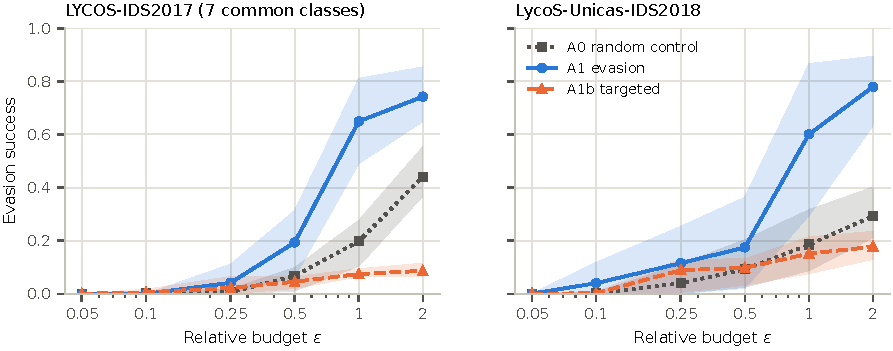
\includegraphics[width=\textwidth]{f_evasion_eps}
  \caption{Constrained evasion success by budget (bands: seed range).}
  \label{f_evasion_eps}
\end{figure*}

% Generated by paper/make_tables_v2.py on 2026-10-30. Do not edit.
% Source: results/stage7/stage7d/cmp2017_seed0_success.csv
% Source: results/stage7/stage7d/cmp2017_seed1_success.csv
% Source: results/stage7/stage7d/cmp2017_seed2_success.csv
% Source: results/stage7/stage7d/seed0/summary_success.csv
% Source: results/stage7/stage7d/seed1/summary_success.csv
% Source: results/stage7/stage7d/seed2/summary_success.csv
\begin{table}[t]
\centering
\footnotesize
\caption{Constrained evasion success by budget, 2017 vs 2018 (7 common classes).}
\label{t_evasion}
\begin{tabular}{lcc}
\toprule
Budget & 2017 mean (seed range) & 2018 mean (seed range) \\
\midrule
\multicolumn{3}{l}{\textit{A0}} \\
$\epsilon = 0.05$ & $0.000$ {\scriptsize ($0.000$ to $0.001$)} & $0.000$ {\scriptsize ($0.000$ to $0.000$)} \\
$\epsilon = 0.10$ & $0.003$ {\scriptsize ($0.000$ to $0.010$)} & $0.002$ {\scriptsize ($0.000$ to $0.005$)} \\
$\epsilon = 0.25$ & $0.006$ {\scriptsize ($0.000$ to $0.018$)} & $0.040$ {\scriptsize ($0.002$ to $0.111$)} \\
$\epsilon = 0.50$ & $0.067$ {\scriptsize ($0.010$ to $0.099$)} & $0.092$ {\scriptsize ($0.025$ to $0.204$)} \\
$\epsilon = 1.00$ & $0.198$ {\scriptsize ($0.104$ to $0.276$)} & $0.185$ {\scriptsize ($0.087$ to $0.317$)} \\
$\epsilon = 2.00$ & $0.439$ {\scriptsize ($0.368$ to $0.554$)} & $0.293$ {\scriptsize ($0.211$ to $0.402$)} \\
\multicolumn{3}{l}{\textit{A1}} \\
$\epsilon = 0.05$ & $0.000$ {\scriptsize ($0.000$ to $0.000$)} & $0.001$ {\scriptsize ($0.001$ to $0.001$)} \\
$\epsilon = 0.10$ & $0.000$ {\scriptsize ($0.000$ to $0.000$)} & $0.040$ {\scriptsize ($0.001$ to $0.118$)} \\
$\epsilon = 0.25$ & $0.042$ {\scriptsize ($0.001$ to $0.111$)} & $0.115$ {\scriptsize ($0.001$ to $0.254$)} \\
$\epsilon = 0.50$ & $0.193$ {\scriptsize ($0.063$ to $0.313$)} & $0.175$ {\scriptsize ($0.021$ to $0.364$)} \\
$\epsilon = 1.00$ & $0.649$ {\scriptsize ($0.490$ to $0.811$)} & $0.601$ {\scriptsize ($0.294$ to $0.866$)} \\
$\epsilon = 2.00$ & $0.742$ {\scriptsize ($0.649$ to $0.854$)} & $0.779$ {\scriptsize ($0.633$ to $0.895$)} \\
\multicolumn{3}{l}{\textit{A1b}} \\
$\epsilon = 0.05$ & $0.000$ {\scriptsize ($0.000$ to $0.001$)} & $0.000$ {\scriptsize ($0.000$ to $0.000$)} \\
$\epsilon = 0.10$ & $0.006$ {\scriptsize ($0.000$ to $0.017$)} & $0.003$ {\scriptsize ($0.000$ to $0.008$)} \\
$\epsilon = 0.25$ & $0.022$ {\scriptsize ($0.000$ to $0.065$)} & $0.089$ {\scriptsize ($0.006$ to $0.130$)} \\
$\epsilon = 0.50$ & $0.045$ {\scriptsize ($0.020$ to $0.065$)} & $0.098$ {\scriptsize ($0.032$ to $0.131$)} \\
$\epsilon = 1.00$ & $0.075$ {\scriptsize ($0.065$ to $0.094$)} & $0.151$ {\scriptsize ($0.076$ to $0.214$)} \\
$\epsilon = 2.00$ & $0.087$ {\scriptsize ($0.065$ to $0.115$)} & $0.177$ {\scriptsize ($0.130$ to $0.235$)} \\
\bottomrule
\end{tabular}
\par\smallskip\parbox{\linewidth}{\scriptsize Success: A0 any change of prediction, A1 predicted benign, A1b predicted as the target class. Macro over the 7 common classes, mean over 3 seeds. $\epsilon = 2$ is the stress setting. A1b targets differ for 3 classes on 2018 (the 2017 targets are absent).}
\end{table}

% Generated by paper/make_tables_v2.py on 2026-10-30. Do not edit.
% Source: results/stage7/stage7c/stage7c_cmp2017_agreement.csv
% Source: results/stage8/clean_variants.csv
\begin{table}[t]
\centering
\footnotesize
\caption{Clean-data agreement, 2017 vs 2018 (7 common classes): Spearman between attention and attribution rankings, all explanation rows (V0) and without near duplicates (V1).}
\label{t_clean_agreement}
\sbox0{%
\begin{tabular}{lcccc}
\toprule
 & \multicolumn{2}{c}{2017} & \multicolumn{2}{c}{2018} \\
Quantity & V0 & V1 & V0 & V1 \\
\midrule
Attn. rollout vs IG & {\begin{tabular}[t]{@{}c@{}}$0.357$\\{\scriptsize ($0.339$ to $0.378$)}\end{tabular}} & {\begin{tabular}[t]{@{}c@{}}$0.349$\\{\scriptsize ($0.317$ to $0.373$)}\end{tabular}} & {\begin{tabular}[t]{@{}c@{}}$0.323$\\{\scriptsize ($0.244$ to $0.423$)}\end{tabular}} & {\begin{tabular}[t]{@{}c@{}}$0.314$\\{\scriptsize ($0.244$ to $0.406$)}\end{tabular}} \\
Attn. rollout vs GradientSHAP & {\begin{tabular}[t]{@{}c@{}}$0.475$\\{\scriptsize ($0.422$ to $0.507$)}\end{tabular}} & {\begin{tabular}[t]{@{}c@{}}$0.470$\\{\scriptsize ($0.412$ to $0.505$)}\end{tabular}} & {\begin{tabular}[t]{@{}c@{}}$0.438$\\{\scriptsize ($0.366$ to $0.523$)}\end{tabular}} & {\begin{tabular}[t]{@{}c@{}}$0.432$\\{\scriptsize ($0.365$ to $0.515$)}\end{tabular}} \\
Attn. rollout vs Occlusion & {\begin{tabular}[t]{@{}c@{}}$0.399$\\{\scriptsize ($0.364$ to $0.433$)}\end{tabular}} & {\begin{tabular}[t]{@{}c@{}}$0.396$\\{\scriptsize ($0.351$ to $0.435$)}\end{tabular}} & {\begin{tabular}[t]{@{}c@{}}$0.367$\\{\scriptsize ($0.314$ to $0.447$)}\end{tabular}} & {\begin{tabular}[t]{@{}c@{}}$0.358$\\{\scriptsize ($0.310$ to $0.429$)}\end{tabular}} \\
Attn. rollout vs TreeSHAP (XGB) & {\begin{tabular}[t]{@{}c@{}}$0.235$\\{\scriptsize ($0.180$ to $0.279$)}\end{tabular}} & {\begin{tabular}[t]{@{}c@{}}$0.231$\\{\scriptsize ($0.176$ to $0.269$)}\end{tabular}} & {\begin{tabular}[t]{@{}c@{}}$0.268$\\{\scriptsize ($0.229$ to $0.330$)}\end{tabular}} & {\begin{tabular}[t]{@{}c@{}}$0.263$\\{\scriptsize ($0.226$ to $0.337$)}\end{tabular}} \\
Attn. layer mean vs IG & {\begin{tabular}[t]{@{}c@{}}$0.314$\\{\scriptsize ($0.289$ to $0.348$)}\end{tabular}} & {\begin{tabular}[t]{@{}c@{}}$0.306$\\{\scriptsize ($0.268$ to $0.340$)}\end{tabular}} & {\begin{tabular}[t]{@{}c@{}}$0.243$\\{\scriptsize ($0.186$ to $0.344$)}\end{tabular}} & {\begin{tabular}[t]{@{}c@{}}$0.238$\\{\scriptsize ($0.190$ to $0.334$)}\end{tabular}} \\
Attn. layer mean vs GradientSHAP & {\begin{tabular}[t]{@{}c@{}}$0.436$\\{\scriptsize ($0.379$ to $0.470$)}\end{tabular}} & {\begin{tabular}[t]{@{}c@{}}$0.431$\\{\scriptsize ($0.369$ to $0.467$)}\end{tabular}} & {\begin{tabular}[t]{@{}c@{}}$0.324$\\{\scriptsize ($0.265$ to $0.435$)}\end{tabular}} & {\begin{tabular}[t]{@{}c@{}}$0.321$\\{\scriptsize ($0.264$ to $0.430$)}\end{tabular}} \\
Attn. layer mean vs Occlusion & {\begin{tabular}[t]{@{}c@{}}$0.351$\\{\scriptsize ($0.313$ to $0.382$)}\end{tabular}} & {\begin{tabular}[t]{@{}c@{}}$0.351$\\{\scriptsize ($0.304$ to $0.387$)}\end{tabular}} & {\begin{tabular}[t]{@{}c@{}}$0.282$\\{\scriptsize ($0.199$ to $0.364$)}\end{tabular}} & {\begin{tabular}[t]{@{}c@{}}$0.276$\\{\scriptsize ($0.196$ to $0.348$)}\end{tabular}} \\
Attn. layer mean vs TreeSHAP (XGB) & {\begin{tabular}[t]{@{}c@{}}$0.209$\\{\scriptsize ($0.154$ to $0.265$)}\end{tabular}} & {\begin{tabular}[t]{@{}c@{}}$0.208$\\{\scriptsize ($0.155$ to $0.259$)}\end{tabular}} & {\begin{tabular}[t]{@{}c@{}}$0.217$\\{\scriptsize ($0.171$ to $0.274$)}\end{tabular}} & {\begin{tabular}[t]{@{}c@{}}$0.215$\\{\scriptsize ($0.155$ to $0.280$)}\end{tabular}} \\
Attn. last layer vs IG & {\begin{tabular}[t]{@{}c@{}}$0.039$\\{\scriptsize ($-0.015$ to $0.103$)}\end{tabular}} & {\begin{tabular}[t]{@{}c@{}}$0.033$\\{\scriptsize ($-0.013$ to $0.092$)}\end{tabular}} & {\begin{tabular}[t]{@{}c@{}}$0.019$\\{\scriptsize ($-0.015$ to $0.050$)}\end{tabular}} & {\begin{tabular}[t]{@{}c@{}}$0.015$\\{\scriptsize ($-0.015$ to $0.048$)}\end{tabular}} \\
Attn. last layer vs GradientSHAP & {\begin{tabular}[t]{@{}c@{}}$0.050$\\{\scriptsize ($-0.032$ to $0.133$)}\end{tabular}} & {\begin{tabular}[t]{@{}c@{}}$0.049$\\{\scriptsize ($-0.023$ to $0.129$)}\end{tabular}} & {\begin{tabular}[t]{@{}c@{}}$0.010$\\{\scriptsize ($-0.050$ to $0.047$)}\end{tabular}} & {\begin{tabular}[t]{@{}c@{}}$0.004$\\{\scriptsize ($-0.052$ to $0.036$)}\end{tabular}} \\
Attn. last layer vs Occlusion & {\begin{tabular}[t]{@{}c@{}}$0.036$\\{\scriptsize ($-0.005$ to $0.082$)}\end{tabular}} & {\begin{tabular}[t]{@{}c@{}}$0.035$\\{\scriptsize ($0.000$ to $0.083$)}\end{tabular}} & {\begin{tabular}[t]{@{}c@{}}$-0.005$\\{\scriptsize ($-0.037$ to $0.045$)}\end{tabular}} & {\begin{tabular}[t]{@{}c@{}}$-0.011$\\{\scriptsize ($-0.048$ to $0.035$)}\end{tabular}} \\
Attn. last layer vs TreeSHAP (XGB) & {\begin{tabular}[t]{@{}c@{}}$0.037$\\{\scriptsize ($-0.018$ to $0.072$)}\end{tabular}} & {\begin{tabular}[t]{@{}c@{}}$0.040$\\{\scriptsize ($-0.002$ to $0.077$)}\end{tabular}} & {\begin{tabular}[t]{@{}c@{}}$0.037$\\{\scriptsize ($0.014$ to $0.073$)}\end{tabular}} & {\begin{tabular}[t]{@{}c@{}}$0.027$\\{\scriptsize ($0.006$ to $0.064$)}\end{tabular}} \\
\bottomrule
\end{tabular}}%
\ifdim\wd0>\textwidth\resizebox{\textwidth}{!}{\usebox0}\else\usebox0\fi
\par\smallskip\parbox{\linewidth}{\scriptsize Macro over the 7 common attack classes, mean over 3 seeds (seed range in brackets). V0: all rows of the clean explanation set, including test rows with a near duplicate in the training set (Table~\ref{t_limitations_data}); V1 (primary): those rows removed.}
\end{table}

% Generated by paper/make_tables_v2.py on 2026-10-30. Do not edit.
% Source: results/stage7/stage7c/stage7c_cmp2017_faithfulness.csv
% Source: results/stage8/clean_variants.csv
% Source: results/stage8/clean_variants_ordering.csv
\begin{table}[t]
\centering
\footnotesize
\caption{Clean-data faithfulness, 2017 vs 2018 (7 common classes), all explanation rows (V0) and without near duplicates (V1).}
\label{t_clean_faith}
\sbox0{%
\begin{tabular}{lcccccc}
\toprule
 & \multicolumn{2}{c}{2017} & \multicolumn{2}{c}{2018} &  &  \\
Quantity & V0 & V1 & V0 & V1 & {\begin{tabular}[t]{@{}c@{}}Rank 2017\\V0 / V1\end{tabular}} & {\begin{tabular}[t]{@{}c@{}}Rank 2018\\V0 / V1\end{tabular}} \\
\midrule
\multicolumn{7}{l}{{\begin{tabular}[t]{@{}l@{}}\textit{Deletion AUC (train-mean masking,}\\\textit{lower is more faithful; rank 1 = lowest)}\end{tabular}}} \\
Attn. rollout & {\begin{tabular}[t]{@{}c@{}}$0.119$\\{\scriptsize ($0.113$ to $0.131$)}\end{tabular}} & {\begin{tabular}[t]{@{}c@{}}$0.125$\\{\scriptsize ($0.114$ to $0.137$)}\end{tabular}} & {\begin{tabular}[t]{@{}c@{}}$0.126$\\{\scriptsize ($0.090$ to $0.189$)}\end{tabular}} & {\begin{tabular}[t]{@{}c@{}}$0.119$\\{\scriptsize ($0.084$ to $0.178$)}\end{tabular}} & $5$ / $5$ & $4$ / $4$ \\
Attn. layer mean & {\begin{tabular}[t]{@{}c@{}}$0.140$\\{\scriptsize ($0.110$ to $0.184$)}\end{tabular}} & {\begin{tabular}[t]{@{}c@{}}$0.145$\\{\scriptsize ($0.111$ to $0.191$)}\end{tabular}} & {\begin{tabular}[t]{@{}c@{}}$0.143$\\{\scriptsize ($0.114$ to $0.199$)}\end{tabular}} & {\begin{tabular}[t]{@{}c@{}}$0.140$\\{\scriptsize ($0.113$ to $0.193$)}\end{tabular}} & $6$ / $6$ & $6$ / $5$ \\
Attn. last layer & {\begin{tabular}[t]{@{}c@{}}$0.239$\\{\scriptsize ($0.214$ to $0.280$)}\end{tabular}} & {\begin{tabular}[t]{@{}c@{}}$0.241$\\{\scriptsize ($0.219$ to $0.272$)}\end{tabular}} & {\begin{tabular}[t]{@{}c@{}}$0.255$\\{\scriptsize ($0.161$ to $0.350$)}\end{tabular}} & {\begin{tabular}[t]{@{}c@{}}$0.259$\\{\scriptsize ($0.174$ to $0.338$)}\end{tabular}} & $7$ / $7$ & $7$ / $7$ \\
IG & {\begin{tabular}[t]{@{}c@{}}$0.020$\\{\scriptsize ($0.015$ to $0.024$)}\end{tabular}} & {\begin{tabular}[t]{@{}c@{}}$0.020$\\{\scriptsize ($0.015$ to $0.024$)}\end{tabular}} & {\begin{tabular}[t]{@{}c@{}}$0.031$\\{\scriptsize ($0.025$ to $0.038$)}\end{tabular}} & {\begin{tabular}[t]{@{}c@{}}$0.031$\\{\scriptsize ($0.025$ to $0.039$)}\end{tabular}} & $1$ / $1$ & $1$ / $1$ \\
GradientSHAP & {\begin{tabular}[t]{@{}c@{}}$0.056$\\{\scriptsize ($0.052$ to $0.058$)}\end{tabular}} & {\begin{tabular}[t]{@{}c@{}}$0.058$\\{\scriptsize ($0.054$ to $0.061$)}\end{tabular}} & {\begin{tabular}[t]{@{}c@{}}$0.054$\\{\scriptsize ($0.044$ to $0.066$)}\end{tabular}} & {\begin{tabular}[t]{@{}c@{}}$0.053$\\{\scriptsize ($0.044$ to $0.065$)}\end{tabular}} & $3$ / $3$ & $3$ / $3$ \\
Occlusion & {\begin{tabular}[t]{@{}c@{}}$0.023$\\{\scriptsize ($0.018$ to $0.032$)}\end{tabular}} & {\begin{tabular}[t]{@{}c@{}}$0.024$\\{\scriptsize ($0.018$ to $0.032$)}\end{tabular}} & {\begin{tabular}[t]{@{}c@{}}$0.049$\\{\scriptsize ($0.032$ to $0.067$)}\end{tabular}} & {\begin{tabular}[t]{@{}c@{}}$0.049$\\{\scriptsize ($0.032$ to $0.067$)}\end{tabular}} & $2$ / $2$ & $2$ / $2$ \\
$|x|$ & {\begin{tabular}[t]{@{}c@{}}$0.075$\\{\scriptsize ($0.070$ to $0.081$)}\end{tabular}} & {\begin{tabular}[t]{@{}c@{}}$0.079$\\{\scriptsize ($0.074$ to $0.084$)}\end{tabular}} & {\begin{tabular}[t]{@{}c@{}}$0.134$\\{\scriptsize ($0.108$ to $0.157$)}\end{tabular}} & {\begin{tabular}[t]{@{}c@{}}$0.149$\\{\scriptsize ($0.122$ to $0.173$)}\end{tabular}} & $4$ / $4$ & $5$ / $6$ \\
Random & {\begin{tabular}[t]{@{}c@{}}$0.242$\\{\scriptsize ($0.236$ to $0.252$)}\end{tabular}} & {\begin{tabular}[t]{@{}c@{}}$0.246$\\{\scriptsize ($0.240$ to $0.258$)}\end{tabular}} & {\begin{tabular}[t]{@{}c@{}}$0.341$\\{\scriptsize ($0.319$ to $0.376$)}\end{tabular}} & {\begin{tabular}[t]{@{}c@{}}$0.345$\\{\scriptsize ($0.323$ to $0.380$)}\end{tabular}} & $8$ / $8$ & $8$ / $8$ \\
{\begin{tabular}[t]{@{}l@{}}\textit{Spearman of the method}\\\textit{ordering, 2017 vs 2018}\end{tabular}} & \multicolumn{6}{c}{V0: $0.976$; V1: $0.929$} \\
\midrule
\multicolumn{7}{l}{{\begin{tabular}[t]{@{}l@{}}\textit{Insertion AUC (train-mean masking,}\\\textit{higher is more faithful; rank 1 = highest)}\end{tabular}}} \\
Attn. rollout & {\begin{tabular}[t]{@{}c@{}}$0.504$\\{\scriptsize ($0.464$ to $0.581$)}\end{tabular}} & {\begin{tabular}[t]{@{}c@{}}$0.501$\\{\scriptsize ($0.460$ to $0.577$)}\end{tabular}} & {\begin{tabular}[t]{@{}c@{}}$0.606$\\{\scriptsize ($0.546$ to $0.680$)}\end{tabular}} & {\begin{tabular}[t]{@{}c@{}}$0.607$\\{\scriptsize ($0.541$ to $0.687$)}\end{tabular}} & $5$ / $5$ & $5$ / $4$ \\
Attn. layer mean & {\begin{tabular}[t]{@{}c@{}}$0.469$\\{\scriptsize ($0.426$ to $0.538$)}\end{tabular}} & {\begin{tabular}[t]{@{}c@{}}$0.470$\\{\scriptsize ($0.420$ to $0.544$)}\end{tabular}} & {\begin{tabular}[t]{@{}c@{}}$0.508$\\{\scriptsize ($0.391$ to $0.569$)}\end{tabular}} & {\begin{tabular}[t]{@{}c@{}}$0.506$\\{\scriptsize ($0.378$ to $0.578$)}\end{tabular}} & $6$ / $6$ & $6$ / $6$ \\
Attn. last layer & {\begin{tabular}[t]{@{}c@{}}$0.251$\\{\scriptsize ($0.191$ to $0.294$)}\end{tabular}} & {\begin{tabular}[t]{@{}c@{}}$0.252$\\{\scriptsize ($0.207$ to $0.285$)}\end{tabular}} & {\begin{tabular}[t]{@{}c@{}}$0.377$\\{\scriptsize ($0.341$ to $0.424$)}\end{tabular}} & {\begin{tabular}[t]{@{}c@{}}$0.374$\\{\scriptsize ($0.328$ to $0.442$)}\end{tabular}} & $7$ / $7$ & $7$ / $7$ \\
IG & {\begin{tabular}[t]{@{}c@{}}$0.749$\\{\scriptsize ($0.726$ to $0.781$)}\end{tabular}} & {\begin{tabular}[t]{@{}c@{}}$0.761$\\{\scriptsize ($0.736$ to $0.793$)}\end{tabular}} & {\begin{tabular}[t]{@{}c@{}}$0.859$\\{\scriptsize ($0.838$ to $0.872$)}\end{tabular}} & {\begin{tabular}[t]{@{}c@{}}$0.864$\\{\scriptsize ($0.837$ to $0.878$)}\end{tabular}} & $1$ / $1$ & $1$ / $1$ \\
GradientSHAP & {\begin{tabular}[t]{@{}c@{}}$0.581$\\{\scriptsize ($0.574$ to $0.588$)}\end{tabular}} & {\begin{tabular}[t]{@{}c@{}}$0.584$\\{\scriptsize ($0.578$ to $0.593$)}\end{tabular}} & {\begin{tabular}[t]{@{}c@{}}$0.790$\\{\scriptsize ($0.770$ to $0.815$)}\end{tabular}} & {\begin{tabular}[t]{@{}c@{}}$0.795$\\{\scriptsize ($0.770$ to $0.817$)}\end{tabular}} & $4$ / $4$ & $3$ / $3$ \\
Occlusion & {\begin{tabular}[t]{@{}c@{}}$0.728$\\{\scriptsize ($0.698$ to $0.779$)}\end{tabular}} & {\begin{tabular}[t]{@{}c@{}}$0.717$\\{\scriptsize ($0.680$ to $0.778$)}\end{tabular}} & {\begin{tabular}[t]{@{}c@{}}$0.795$\\{\scriptsize ($0.778$ to $0.810$)}\end{tabular}} & {\begin{tabular}[t]{@{}c@{}}$0.795$\\{\scriptsize ($0.782$ to $0.812$)}\end{tabular}} & $2$ / $2$ & $2$ / $2$ \\
$|x|$ & {\begin{tabular}[t]{@{}c@{}}$0.638$\\{\scriptsize ($0.627$ to $0.650$)}\end{tabular}} & {\begin{tabular}[t]{@{}c@{}}$0.636$\\{\scriptsize ($0.629$ to $0.649$)}\end{tabular}} & {\begin{tabular}[t]{@{}c@{}}$0.610$\\{\scriptsize ($0.566$ to $0.661$)}\end{tabular}} & {\begin{tabular}[t]{@{}c@{}}$0.604$\\{\scriptsize ($0.560$ to $0.656$)}\end{tabular}} & $3$ / $3$ & $4$ / $5$ \\
Random & {\begin{tabular}[t]{@{}c@{}}$0.243$\\{\scriptsize ($0.238$ to $0.253$)}\end{tabular}} & {\begin{tabular}[t]{@{}c@{}}$0.246$\\{\scriptsize ($0.239$ to $0.257$)}\end{tabular}} & {\begin{tabular}[t]{@{}c@{}}$0.338$\\{\scriptsize ($0.317$ to $0.374$)}\end{tabular}} & {\begin{tabular}[t]{@{}c@{}}$0.342$\\{\scriptsize ($0.320$ to $0.379$)}\end{tabular}} & $8$ / $8$ & $8$ / $8$ \\
{\begin{tabular}[t]{@{}l@{}}\textit{Spearman of the method}\\\textit{ordering, 2017 vs 2018}\end{tabular}} & \multicolumn{6}{c}{V0: $0.976$; V1: $0.929$} \\
\bottomrule
\end{tabular}}%
\ifdim\wd0>\textwidth\resizebox{\textwidth}{!}{\usebox0}\else\usebox0\fi
\par\smallskip\parbox{\linewidth}{\scriptsize Macro over the 7 common attack classes, mean over 3 seeds (seed range in brackets). Ranks: position of each method among the 8 methods, computed from the 7-class means, separately per metric, dataset and row set. The last row of each block is the Spearman correlation of the 2017 and 2018 rankings. V0: all rows of the clean explanation set, including test rows with a near duplicate in the training set (Table~\ref{t_limitations_data}); V1 (primary): those rows removed.}
\end{table}

% Generated by paper/make_tables_v2.py on 2026-10-30. Do not edit.
% Source: results/stage7/stage7d/cmp2017_seed0_success.csv
% Source: results/stage7/stage7d/cmp2017_seed1_success.csv
% Source: results/stage7/stage7d/cmp2017_seed2_success.csv
% Source: results/stage7/stage7d/seed0/summary_success.csv
% Source: results/stage7/stage7d/seed1/summary_success.csv
% Source: results/stage7/stage7d/seed2/summary_success.csv
% Source: results/stage7/stage7d/cmp2017_seed0_faith_excess_vs_A0.csv
% Source: results/stage7/stage7d/cmp2017_seed1_faith_excess_vs_A0.csv
% Source: results/stage7/stage7d/cmp2017_seed2_faith_excess_vs_A0.csv
% Source: results/stage7/stage7d/seed0/summary_faith_excess_vs_A0.csv
% Source: results/stage7/stage7d/seed1/summary_faith_excess_vs_A0.csv
% Source: results/stage7/stage7d/seed2/summary_faith_excess_vs_A0.csv
% Source: results/stage8/sensitivity_stage5.csv
\begin{table}[t]
\centering
\footnotesize
\caption{Attention under constrained attacks, 2017 vs 2018 (7 common classes), all source rows (V0) and without near duplicates (V1).}
\label{t_faith_attack}
\sbox0{%
\begin{tabular}{lccc}
\toprule
 & \multicolumn{2}{c}{2017} & 2018 \\
Quantity & V0 & V1 & V0 = V1 \\
\midrule
\multicolumn{4}{l}{\textit{Top-10 rollout mass ratio adversarial / clean (1 = unchanged)}} \\
A2, $\epsilon = 0.25$ & $0.975$ {\scriptsize ($0.962$ to $0.983$)} & $0.975$ {\scriptsize ($0.961$ to $0.984$)} & $0.945$ {\scriptsize ($0.936$ to $0.960$)} \\
A2, $\epsilon = 0.50$ & $0.943$ {\scriptsize ($0.915$ to $0.963$)} & $0.946$ {\scriptsize ($0.911$ to $0.967$)} & $0.917$ {\scriptsize ($0.907$ to $0.927$)} \\
A2, $\epsilon = 1.00$ & $0.902$ {\scriptsize ($0.870$ to $0.943$)} & $0.906$ {\scriptsize ($0.864$ to $0.948$)} & $0.861$ {\scriptsize ($0.840$ to $0.874$)} \\
A3 $\lambda{=}100$, $\epsilon = 0.25$ & $0.976$ {\scriptsize ($0.963$ to $0.983$)} & $0.977$ {\scriptsize ($0.964$ to $0.984$)} & $0.955$ {\scriptsize ($0.945$ to $0.963$)} \\
A3 $\lambda{=}100$, $\epsilon = 0.50$ & $0.942$ {\scriptsize ($0.911$ to $0.971$)} & $0.946$ {\scriptsize ($0.910$ to $0.972$)} & $0.932$ {\scriptsize ($0.924$ to $0.941$)} \\
A3 $\lambda{=}100$, $\epsilon = 1.00$ & $0.915$ {\scriptsize ($0.875$ to $0.981$)} & $0.919$ {\scriptsize ($0.873$ to $0.986$)} & $0.886$ {\scriptsize ($0.874$ to $0.902$)} \\
A3 $\lambda{=}1000$, $\epsilon = 0.25$ & $0.974$ {\scriptsize ($0.960$ to $0.983$)} & $0.974$ {\scriptsize ($0.958$ to $0.984$)} & $0.952$ {\scriptsize ($0.939$ to $0.960$)} \\
A3 $\lambda{=}1000$, $\epsilon = 0.50$ & $0.938$ {\scriptsize ($0.904$ to $0.963$)} & $0.941$ {\scriptsize ($0.898$ to $0.966$)} & $0.926$ {\scriptsize ($0.917$ to $0.941$)} \\
A3 $\lambda{=}1000$, $\epsilon = 1.00$ & $0.896$ {\scriptsize ($0.861$ to $0.940$)} & $0.900$ {\scriptsize ($0.855$ to $0.947$)} & $0.869$ {\scriptsize ($0.854$ to $0.885$)} \\
A3 norm., $\epsilon = 0.25$ & $0.982$ {\scriptsize ($0.975$ to $0.987$)} & $0.983$ {\scriptsize ($0.975$ to $0.990$)} & $0.977$ {\scriptsize ($0.969$ to $0.982$)} \\
A3 norm., $\epsilon = 0.50$ & $0.957$ {\scriptsize ($0.940$ to $0.990$)} & $0.961$ {\scriptsize ($0.940$ to $0.991$)} & $0.973$ {\scriptsize ($0.958$ to $0.995$)} \\
A3 norm., $\epsilon = 1.00$ & $0.947$ {\scriptsize ($0.907$ to $1.023$)} & $0.950$ {\scriptsize ($0.908$ to $1.024$)} & $0.951$ {\scriptsize ($0.925$ to $0.984$)} \\
{\begin{tabular}[t]{@{}l@{}}A2 unconstrained reference,\\standardised $\epsilon = 0.5$\end{tabular}} & $0.796$ {\scriptsize ($0.746$ to $0.834$)} & $0.800$ {\scriptsize ($0.748$ to $0.833$)} & $0.726$ {\scriptsize ($0.699$ to $0.743$)} \\
\midrule
\multicolumn{4}{l}{\textit{Evasion success, A1 minus A0}} \\
$\epsilon = 0.25$ & $0.035$ {\scriptsize ($-0.006$ to $0.110$)} & $0.011$ {\scriptsize ($-0.022$ to $0.055$)} & $0.076$ {\scriptsize ($-0.001$ to $0.143$)} \\
$\epsilon = 0.50$ & $0.126$ {\scriptsize ($0.052$ to $0.221$)} & $0.089$ {\scriptsize ($0.002$ to $0.228$)} & $0.082$ {\scriptsize ($-0.004$ to $0.160$)} \\
$\epsilon = 1.00$ & $0.451$ {\scriptsize ($0.276$ to $0.543$)} & $0.416$ {\scriptsize ($0.216$ to $0.544$)} & $0.416$ {\scriptsize ($0.207$ to $0.550$)} \\
\midrule
\multicolumn{4}{l}{{\begin{tabular}[t]{@{}l@{}}\textit{Flipped A1 rows, $\epsilon = 1$: margin AOPC gap change vs clean,}\\\textit{minus the A0 change}\end{tabular}}} \\
IG & $-10.70$ {\scriptsize ($-12.78$ to $-8.83$)} & $-11.06$ {\scriptsize ($-13.04$ to $-9.02$)} & $-11.36$ {\scriptsize ($-12.05$ to $-10.99$)} \\
Occlusion & $-12.29$ {\scriptsize ($-14.15$ to $-10.38$)} & $-12.55$ {\scriptsize ($-14.26$ to $-10.83$)} & $-10.61$ {\scriptsize ($-10.88$ to $-10.25$)} \\
Static IG (class mean) & $-9.66$ {\scriptsize ($-11.15$ to $-7.67$)} & $-9.72$ {\scriptsize ($-11.09$ to $-7.72$)} & $-10.07$ {\scriptsize ($-10.57$ to $-9.59$)} \\
Attn. rollout & $-7.61$ {\scriptsize ($-8.90$ to $-6.23$)} & $-7.45$ {\scriptsize ($-8.09$ to $-6.59$)} & $-7.50$ {\scriptsize ($-8.93$ to $-5.84$)} \\
Attn. layer mean & $-7.13$ {\scriptsize ($-8.41$ to $-5.88$)} & $-7.16$ {\scriptsize ($-8.00$ to $-6.15$)} & $-7.37$ {\scriptsize ($-7.74$ to $-6.65$)} \\
Attn. last layer & $0.31$ {\scriptsize ($-1.78$ to $3.68$)} & $1.04$ {\scriptsize ($-1.33$ to $4.31$)} & $-1.16$ {\scriptsize ($-2.92$ to $0.34$)} \\
Static rollout (class mean) & $-5.49$ {\scriptsize ($-5.98$ to $-4.56$)} & $-5.43$ {\scriptsize ($-6.16$ to $-4.63$)} & $-6.19$ {\scriptsize ($-7.39$ to $-4.99$)} \\
$|x|$ & $-6.14$ {\scriptsize ($-7.69$ to $-4.94$)} & $-6.60$ {\scriptsize ($-8.94$ to $-4.86$)} & $-5.97$ {\scriptsize ($-6.61$ to $-5.56$)} \\
Random & $0.10$ {\scriptsize ($0.04$ to $0.19$)} & $0.02$ {\scriptsize ($-0.10$ to $0.15$)} & $0.25$ {\scriptsize ($-0.31$ to $0.82$)} \\
\bottomrule
\end{tabular}}%
\ifdim\wd0>\textwidth\resizebox{\textwidth}{!}{\usebox0}\else\usebox0\fi
\par\smallskip\parbox{\linewidth}{\scriptsize Macro over the 7 common classes, mean over 3 seeds (seed range in brackets). V0: all source rows; V1 (primary): source rows with a near duplicate in the training set removed; on 2018 no source row is flagged, so V1 equals V0. A2 keeps the prediction and minimises rollout mass on the clean top-10 IG features; A3 also evades. Margin AOPC gap: logit margin; more negative = larger loss of faithfulness. Static rankings are fixed train-set class means.}
\end{table}

% Generated by paper/make_tables_v2.py on 2026-10-30. Do not edit.
% Source: results/stage6/final/seed{0,1,2}/rows_eps*_*.parquet and results/stage6/strong/seed{0,1,2}/rows_eps1_A8*.parquet (7 common classes)
% Source: results/stage7/stage7e/seed{0,1,2}/rows_eps*_*.parquet
\begin{table}[t]
\centering
\footnotesize
\setlength{\tabcolsep}{4pt}
\caption{Success AND undetected under D and D$_+$ at $\epsilon = 1$, 2017 vs 2018 (7 common classes).}
\label{t_defenders}
\begin{tabular}{lcccccc}
\toprule
 & \multicolumn{3}{c}{2017} & \multicolumn{3}{c}{2018} \\
Attack & Success & Undet. D & Undet. D$_+$ & Success & Undet. D & Undet. D$_+$ \\
\midrule
A1 & {\begin{tabular}[t]{@{}c@{}}$0.648$\\{\scriptsize ($0.489$ to $0.810$)}\end{tabular}} & {\begin{tabular}[t]{@{}c@{}}$0.013$\\{\scriptsize ($0.000$ to $0.039$)}\end{tabular}} & {\begin{tabular}[t]{@{}c@{}}$0.001$\\{\scriptsize ($0.000$ to $0.003$)}\end{tabular}} & {\begin{tabular}[t]{@{}c@{}}$0.584$\\{\scriptsize ($0.266$ to $0.863$)}\end{tabular}} & {\begin{tabular}[t]{@{}c@{}}$0.001$\\{\scriptsize ($0.000$ to $0.001$)}\end{tabular}} & {\begin{tabular}[t]{@{}c@{}}$0.000$\\{\scriptsize ($0.000$ to $0.001$)}\end{tabular}} \\
A6 $\lambda{=}1$ & {\begin{tabular}[t]{@{}c@{}}$0.533$\\{\scriptsize ($0.316$ to $0.740$)}\end{tabular}} & {\begin{tabular}[t]{@{}c@{}}$0.185$\\{\scriptsize ($0.127$ to $0.250$)}\end{tabular}} & {\begin{tabular}[t]{@{}c@{}}$0.079$\\{\scriptsize ($0.008$ to $0.194$)}\end{tabular}} & {\begin{tabular}[t]{@{}c@{}}$0.303$\\{\scriptsize ($0.129$ to $0.504$)}\end{tabular}} & {\begin{tabular}[t]{@{}c@{}}$0.014$\\{\scriptsize ($0.002$ to $0.036$)}\end{tabular}} & {\begin{tabular}[t]{@{}c@{}}$0.002$\\{\scriptsize ($0.000$ to $0.007$)}\end{tabular}} \\
A6 $\lambda{=}100$ & {\begin{tabular}[t]{@{}c@{}}$0.342$\\{\scriptsize ($0.141$ to $0.519$)}\end{tabular}} & {\begin{tabular}[t]{@{}c@{}}$0.116$\\{\scriptsize ($0.006$ to $0.213$)}\end{tabular}} & {\begin{tabular}[t]{@{}c@{}}$0.049$\\{\scriptsize ($0.001$ to $0.125$)}\end{tabular}} & {\begin{tabular}[t]{@{}c@{}}$0.280$\\{\scriptsize ($0.092$ to $0.481$)}\end{tabular}} & {\begin{tabular}[t]{@{}c@{}}$0.006$\\{\scriptsize ($0.001$ to $0.014$)}\end{tabular}} & {\begin{tabular}[t]{@{}c@{}}$0.003$\\{\scriptsize ($0.000$ to $0.008$)}\end{tabular}} \\
A6 norm. & {\begin{tabular}[t]{@{}c@{}}$0.653$\\{\scriptsize ($0.585$ to $0.759$)}\end{tabular}} & {\begin{tabular}[t]{@{}c@{}}$0.160$\\{\scriptsize ($0.084$ to $0.273$)}\end{tabular}} & {\begin{tabular}[t]{@{}c@{}}$0.050$\\{\scriptsize ($0.005$ to $0.125$)}\end{tabular}} & {\begin{tabular}[t]{@{}c@{}}$0.493$\\{\scriptsize ($0.281$ to $0.722$)}\end{tabular}} & {\begin{tabular}[t]{@{}c@{}}$0.013$\\{\scriptsize ($0.001$ to $0.025$)}\end{tabular}} & {\begin{tabular}[t]{@{}c@{}}$0.000$\\{\scriptsize ($0.000$ to $0.001$)}\end{tabular}} \\
A8 $\lambda{=}1$ & {\begin{tabular}[t]{@{}c@{}}$0.566$\\{\scriptsize ($0.379$ to $0.763$)}\end{tabular}} & {\begin{tabular}[t]{@{}c@{}}$0.141$\\{\scriptsize ($0.116$ to $0.169$)}\end{tabular}} & {\begin{tabular}[t]{@{}c@{}}$0.132$\\{\scriptsize ($0.060$ to $0.267$)}\end{tabular}} & {\begin{tabular}[t]{@{}c@{}}$0.335$\\{\scriptsize ($0.123$ to $0.602$)}\end{tabular}} & {\begin{tabular}[t]{@{}c@{}}$0.007$\\{\scriptsize ($0.001$ to $0.016$)}\end{tabular}} & {\begin{tabular}[t]{@{}c@{}}$0.013$\\{\scriptsize ($0.001$ to $0.020$)}\end{tabular}} \\
A8 $\lambda{=}100$ & {\begin{tabular}[t]{@{}c@{}}$0.474$\\{\scriptsize ($0.264$ to $0.673$)}\end{tabular}} & {\begin{tabular}[t]{@{}c@{}}$0.105$\\{\scriptsize ($0.021$ to $0.157$)}\end{tabular}} & {\begin{tabular}[t]{@{}c@{}}$0.127$\\{\scriptsize ($0.011$ to $0.298$)}\end{tabular}} & {\begin{tabular}[t]{@{}c@{}}$0.324$\\{\scriptsize ($0.131$ to $0.552$)}\end{tabular}} & {\begin{tabular}[t]{@{}c@{}}$0.007$\\{\scriptsize ($0.000$ to $0.019$)}\end{tabular}} & {\begin{tabular}[t]{@{}c@{}}$0.013$\\{\scriptsize ($0.001$ to $0.018$)}\end{tabular}} \\
A8 norm. & {\begin{tabular}[t]{@{}c@{}}$0.658$\\{\scriptsize ($0.561$ to $0.794$)}\end{tabular}} & {\begin{tabular}[t]{@{}c@{}}$0.106$\\{\scriptsize ($0.059$ to $0.165$)}\end{tabular}} & {\begin{tabular}[t]{@{}c@{}}$0.114$\\{\scriptsize ($0.033$ to $0.277$)}\end{tabular}} & {\begin{tabular}[t]{@{}c@{}}$0.504$\\{\scriptsize ($0.237$ to $0.748$)}\end{tabular}} & {\begin{tabular}[t]{@{}c@{}}$0.000$\\{\scriptsize ($0.000$ to $0.001$)}\end{tabular}} & {\begin{tabular}[t]{@{}c@{}}$0.006$\\{\scriptsize ($0.000$ to $0.011$)}\end{tabular}} \\
\bottomrule
\end{tabular}
\par\smallskip\parbox{\linewidth}{\scriptsize Fraction of source rows predicted benign (Success) and also below the detector threshold set at 5\% FPR on validation benign rows (Undet.). Mean over seeds pooled over rows, seed range in brackets. A6 targets D, A8 targets D$_+$. Defenders: 2017 ($\epsilon = 1.0$; D / D$_+$): seed 0: val AUROC 0.988 / 0.993, test FPR 0.055 / 0.057, trained on 854 positives and 20{,}000 negatives; seed 1: val AUROC 0.996 / 0.998, test FPR 0.056 / 0.054, trained on 649 positives and 20{,}000 negatives; seed 2: val AUROC 0.990 / 0.996, test FPR 0.045 / 0.047, trained on 538 positives and 20{,}000 negatives. 2018 ($\epsilon = 1.0$; D / D$_+$): seed 0: val AUROC 0.996 / 0.999, test FPR 0.053 / 0.044, trained on 228 positives and 20{,}000 negatives; seed 1: val AUROC 0.995 / 0.997, test FPR 0.058 / 0.051, trained on 566 positives and 20{,}000 negatives; seed 2: val AUROC 0.999 / 1.000, test FPR 0.053 / 0.053, trained on 448 positives and 20{,}000 negatives.}
\end{table}

% Generated by paper/make_tables_v2.py on 2026-10-30. Do not edit.
% Source: results/stage6/final/seed{0,1,2}/rows_eps*_*.parquet and results/stage6/strong/seed{0,1,2}/rows_eps1_A8*.parquet (7 common classes)
% Source: results/stage7/stage7e/summary_pooled_per_class_attacks.csv
\begin{table}[t]
\centering
\footnotesize
\setlength{\tabcolsep}{4pt}
\caption{Per-class share of successful and undetected source rows at $\epsilon = 1$: A6 $\lambda{=}1$ vs D, A8 $\lambda{=}1$ vs D$_+$.}
\label{t_per_class}
\begin{tabular}{lcccccc}
\toprule
 & \multicolumn{3}{c}{2017} & \multicolumn{3}{c}{2018} \\
Class & A6 vs D & A8 vs D$_+$ & n & A6 vs D & A8 vs D$_+$ & n \\
\midrule
Bot & {\begin{tabular}[t]{@{}c@{}}$0.824$\\{\scriptsize ($0.611$ to $0.944$)}\end{tabular}} & {\begin{tabular}[t]{@{}c@{}}$0.493$\\{\scriptsize ($0.340$ to $0.646$)}\end{tabular}} & 144 & {\begin{tabular}[t]{@{}c@{}}$0.000$\\{\scriptsize ($0.000$ to $0.000$)}\end{tabular}} & {\begin{tabular}[t]{@{}c@{}}$0.000$\\{\scriptsize ($0.000$ to $0.000$)}\end{tabular}} & 150 \\
DDoS & {\begin{tabular}[t]{@{}c@{}}$0.000$\\{\scriptsize ($0.000$ to $0.000$)}\end{tabular}} & {\begin{tabular}[t]{@{}c@{}}$0.000$\\{\scriptsize ($0.000$ to $0.000$)}\end{tabular}} & 150 & {\begin{tabular}[t]{@{}c@{}}$0.080$\\{\scriptsize ($0.000$ to $0.233$)}\end{tabular}} & {\begin{tabular}[t]{@{}c@{}}$0.080$\\{\scriptsize ($0.000$ to $0.133$)}\end{tabular}} & 150 \\
DoS GoldenEye & {\begin{tabular}[t]{@{}c@{}}$0.078$\\{\scriptsize ($0.000$ to $0.227$)}\end{tabular}} & {\begin{tabular}[t]{@{}c@{}}$0.082$\\{\scriptsize ($0.000$ to $0.240$)}\end{tabular}} & 150 & {\begin{tabular}[t]{@{}c@{}}$0.000$\\{\scriptsize ($0.000$ to $0.000$)}\end{tabular}} & {\begin{tabular}[t]{@{}c@{}}$0.000$\\{\scriptsize ($0.000$ to $0.000$)}\end{tabular}} & 150 \\
DoS Hulk & {\begin{tabular}[t]{@{}c@{}}$0.067$\\{\scriptsize ($0.000$ to $0.160$)}\end{tabular}} & {\begin{tabular}[t]{@{}c@{}}$0.038$\\{\scriptsize ($0.000$ to $0.107$)}\end{tabular}} & 150 & {\begin{tabular}[t]{@{}c@{}}$0.000$\\{\scriptsize ($0.000$ to $0.000$)}\end{tabular}} & {\begin{tabular}[t]{@{}c@{}}$0.000$\\{\scriptsize ($0.000$ to $0.000$)}\end{tabular}} & 150 \\
DoS Slowloris & {\begin{tabular}[t]{@{}c@{}}$0.000$\\{\scriptsize ($0.000$ to $0.000$)}\end{tabular}} & {\begin{tabular}[t]{@{}c@{}}$0.000$\\{\scriptsize ($0.000$ to $0.000$)}\end{tabular}} & 150 & {\begin{tabular}[t]{@{}c@{}}$0.002$\\{\scriptsize ($0.000$ to $0.007$)}\end{tabular}} & {\begin{tabular}[t]{@{}c@{}}$0.002$\\{\scriptsize ($0.000$ to $0.007$)}\end{tabular}} & 150 \\
SSH-Patator & {\begin{tabular}[t]{@{}c@{}}$0.187$\\{\scriptsize ($0.000$ to $0.487$)}\end{tabular}} & {\begin{tabular}[t]{@{}c@{}}$0.176$\\{\scriptsize ($0.000$ to $0.473$)}\end{tabular}} & 150 & {\begin{tabular}[t]{@{}c@{}}$0.004$\\{\scriptsize ($0.000$ to $0.013$)}\end{tabular}} & {\begin{tabular}[t]{@{}c@{}}$0.000$\\{\scriptsize ($0.000$ to $0.000$)}\end{tabular}} & 150 \\
Web attack & {\begin{tabular}[t]{@{}c@{}}$0.162$\\{\scriptsize ($0.000$ to $0.280$)}\end{tabular}} & {\begin{tabular}[t]{@{}c@{}}$0.151$\\{\scriptsize ($0.000$ to $0.420$)}\end{tabular}} & 150 & {\begin{tabular}[t]{@{}c@{}}$0.004$\\{\scriptsize ($0.000$ to $0.012$)}\end{tabular}} & {\begin{tabular}[t]{@{}c@{}}$0.000$\\{\scriptsize ($0.000$ to $0.000$)}\end{tabular}} & 85$^\ast$ \\
\bottomrule
\end{tabular}
\par\smallskip\parbox{\linewidth}{\scriptsize n: source rows per seed; $^\ast$ marks n < 100. Seed range in brackets. 2018 DoS Slowloris uses only rows without a near duplicate in the training set.}
\end{table}


\begin{figure*}[!tbp]
  \centering
  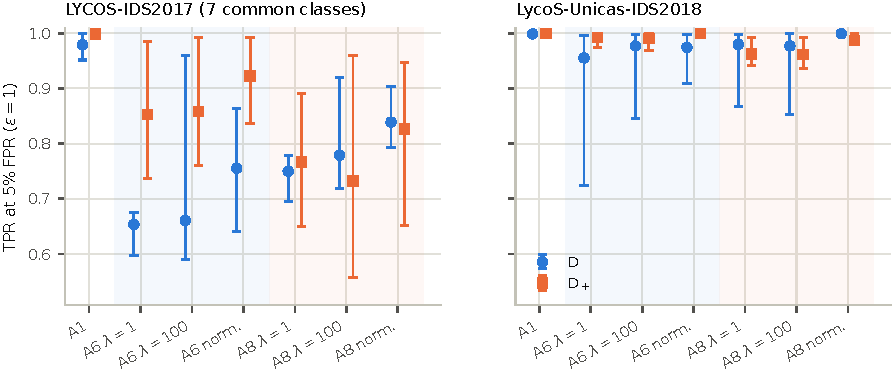
\includegraphics[width=\textwidth]{f_detection_tpr}
  \caption{TPR at \paramFPR{} FPR of D and D$_+$ per attack at $\epsilon = \paramEpsHead$, all source rows (V0); D$_+$
    against the stand-in attacker A8 (error bars: seed range).}
  \label{f_detection_tpr}
\end{figure*}

\begin{figure}[!tbp]
  \centering
  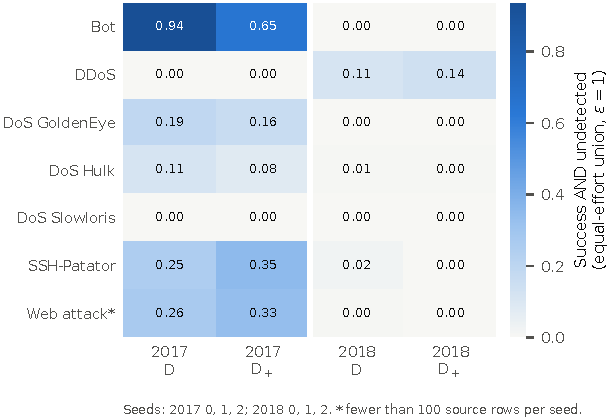
\includegraphics[width=\columnwidth]{f_per_class_heatmap}
  \caption{Per-class share of successful and undetected source rows under the equal-effort union at
    $\epsilon = \paramEpsHead$, all source rows (V0); D$_+$ against the stand-in attacker A8.}
  \label{f_per_class_heatmap}
\end{figure}

% Generated by paper_v3/gen/make_tables_v3.py on 2026-10-30. Do not edit.
% Source: results/stage9/a8x/summary_union.csv
% Source: results/stage9/adaptive/summary_union.csv
\begin{table}[t]
\centering
\footnotesize
\setlength{\tabcolsep}{4pt}
\caption{Against the stand-in attacker A8: equal-effort union with D$_+$ facing A1 + A8 $\times 3$ ($\epsilon = 1$), and the controls compared with D$_+$ under A8.}
\label{t_union_a8}
\textit{D$_+$ minus D, D$_+$ against A8}\par\smallskip
\sbox0{%
\begin{tabular}{llcccc}
\toprule
Dataset & Rows & Undet. D & Undet. D$_+$ & D$_+$ minus D [95\% CI] & Seeds 0 / 1 / 2 \\
\midrule
2017 & V0 & $0.246$ & $0.221$ & $-0.025$ {\scriptsize [$-0.039$, $-0.012$]} & $+0.063\,/\,-0.050\,/\,-0.089$ \\
2017 & V1 & $0.266$ & $0.229$ & $-0.037$ {\scriptsize [$-0.051$, $-0.023$]} & $+0.031\,/\,-0.058\,/\,-0.084$ \\
2017 & V2 & $0.293$ & $0.244$ & $-0.049$ {\scriptsize [$-0.064$, $-0.032$]} & $-0.004\,/\,-0.071\,/\,-0.071$ \\
\midrule
2018 & V0 & $0.023$ & $0.022$ & $-0.001$ {\scriptsize [$-0.008$, $+0.006$]} & $-0.050\,/\,+0.029\,/\,+0.018$ \\
2018 & V1 & $0.023$ & $0.022$ & $-0.001$ {\scriptsize [$-0.008$, $+0.007$]} & $-0.050\,/\,+0.029\,/\,+0.018$ \\
2018 & V2 & $0.029$ & $0.028$ & $0.000$ {\scriptsize [$-0.011$, $+0.009$]} & $-0.067\,/\,+0.040\,/\,+0.025$ \\
\bottomrule
\end{tabular}}%
\ifdim\wd0>\textwidth\resizebox{\textwidth}{!}{\usebox0}\else\usebox0\fi
\par\medskip
\textit{Control minus D$_+$, D$_+$ against A8 (V1)}\par\smallskip
\sbox0{%
\begin{tabular}{lllcccc}
\toprule
Dataset & Control & Attacker & Undet. control & Undet. D$_+$ & Minus D$_+$ [95\% CI] & Seeds 0 / 1 / 2 \\
\midrule
2017 & c0 & exact & $0.266$ & $0.229$ & $+0.037$ {\scriptsize [$+0.024$, $+0.052$]} & $-0.036\,/\,+0.060\,/\,+0.088$ \\
2017 & c1 & exact & $0.280$ & $0.229$ & $+0.051$ {\scriptsize [$+0.038$, $+0.066$]} & $-0.020\,/\,+0.057\,/\,+0.117$ \\
2017 & c2 & exact & $0.273$ & $0.229$ & $+0.045$ {\scriptsize [$+0.030$, $+0.060$]} & $-0.107\,/\,+0.139\,/\,+0.102$ \\
2017 & a1 & stand-in & $0.344$ & $0.229$ & $+0.115$ {\scriptsize [$+0.100$, $+0.130$]} & $+0.175\,/\,-0.054\,/\,+0.225$ \\
2017 & a2 & stand-in & $0.278$ & $0.229$ & $+0.050$ {\scriptsize [$+0.035$, $+0.065$]} & $-0.062\,/\,+0.026\,/\,+0.185$ \\
\midrule
2018 & c0 & exact & $0.015$ & $0.022$ & $-0.007$ {\scriptsize [$-0.014$, $-0.001$]} & $+0.041\,/\,-0.029\,/\,-0.034$ \\
2018 & c1 & exact & $0.019$ & $0.022$ & $-0.003$ {\scriptsize [$-0.009$, $+0.004$]} & $+0.044\,/\,-0.019\,/\,-0.034$ \\
2018 & c2 & exact & $0.055$ & $0.022$ & $+0.033$ {\scriptsize [$+0.024$, $+0.042$]} & $+0.001\,/\,+0.132\,/\,-0.034$ \\
2018 & a1 & stand-in & $0.006$ & $0.022$ & $-0.016$ {\scriptsize [$-0.021$, $-0.010$]} & $+0.010\,/\,-0.023\,/\,-0.034$ \\
2018 & a2 & stand-in & $0.021$ & $0.022$ & $-0.001$ {\scriptsize [$-0.007$, $+0.006$]} & $+0.040\,/\,-0.009\,/\,-0.032$ \\
\bottomrule
\end{tabular}}%
\ifdim\wd0>\textwidth\resizebox{\textwidth}{!}{\usebox0}\else\usebox0\fi
\par\smallskip\parbox{\linewidth}{\scriptsize D faces A1 + A6 $\times 3$. Paired bootstrap over source rows within seed (1,000 draws). These comparisons use the stand-in attacker A8 for D$_+$; against the exact-objective attacker A8x the sign of D$_+$ minus D reversed (Table~\ref{t_union_adaptive}), so the control minus D$_+$ values here are not the comparison at the stronger attacker.}
\end{table}

% Generated by paper_v3/gen/make_tables_v3.py on 2026-10-30. Do not edit.
% Source: results/stage9/a8x/summary_union.csv
% Source: results/stage9/a6x/summary_union.csv
\begin{table}[t]
\centering
\footnotesize
\setlength{\tabcolsep}{4pt}
\caption{D$_+$ minus D under A8x per attack setting, the unequal-effort sensitivity unions and the A6x union (V1, $\epsilon = 1$).}
\label{t_a8x_setting}
\sbox0{%
\begin{tabular}{llcc}
\toprule
Dataset & Union & D$_+$ minus D [95\% CI] & Seeds 0 / 1 / 2 \\
\midrule
2017 & A8x $\lambda{=}1$ vs A6 $\lambda{=}1$ & $+0.074$ {\scriptsize [$+0.059$, $+0.090$]} & $+0.152\,/\,-0.051\,/\,+0.121$ \\
2017 & A8x $\lambda{=}100$ vs A6 $\lambda{=}100$ & $+0.115$ {\scriptsize [$+0.099$, $+0.131$]} & $+0.204\,/\,+0.013\,/\,+0.128$ \\
2017 & A8x norm. vs A6 norm. & $+0.071$ {\scriptsize [$+0.054$, $+0.087$]} & $+0.169\,/\,-0.047\,/\,+0.090$ \\
2017 & Unequal effort: D$_+$ faces A1 + A8 $\times 3$ + A8x $\times 3$ & $+0.088$ {\scriptsize [$+0.074$, $+0.102$]} & $+0.137\,/\,-0.029\,/\,+0.155$ \\
2017 & A6x headline: D faces A1 + A6x $\times 3$ & $+0.075$ {\scriptsize [$+0.061$, $+0.090$]} & $+0.114\,/\,-0.037\,/\,+0.149$ \\
2017 & Unequal effort: D faces A1 + A6 $\times 3$ + A6x $\times 3$ & $+0.075$ {\scriptsize [$+0.061$, $+0.090$]} & $+0.114\,/\,-0.037\,/\,+0.149$ \\
\midrule
2018 & A8x $\lambda{=}1$ vs A6 $\lambda{=}1$ & $+0.007$ {\scriptsize [$+0.000$, $+0.014$]} & $-0.035\,/\,+0.016\,/\,+0.041$ \\
2018 & A8x $\lambda{=}100$ vs A6 $\lambda{=}100$ & $+0.012$ {\scriptsize [$+0.006$, $+0.018$]} & $-0.014\,/\,+0.010\,/\,+0.040$ \\
2018 & A8x norm. vs A6 norm. & $+0.003$ {\scriptsize [$-0.003$, $+0.009$]} & $-0.025\,/\,+0.026\,/\,+0.009$ \\
2018 & Unequal effort: D$_+$ faces A1 + A8 $\times 3$ + A8x $\times 3$ & $+0.016$ {\scriptsize [$+0.007$, $+0.024$]} & $-0.049\,/\,+0.053\,/\,+0.044$ \\
2018 & A6x headline: D faces A1 + A6x $\times 3$ & $+0.009$ {\scriptsize [$+0.001$, $+0.017$]} & $-0.050\,/\,+0.040\,/\,+0.039$ \\
2018 & Unequal effort: D faces A1 + A6 $\times 3$ + A6x $\times 3$ & $+0.009$ {\scriptsize [$+0.001$, $+0.018$]} & $-0.050\,/\,+0.040\,/\,+0.039$ \\
\bottomrule
\end{tabular}}%
\ifdim\wd0>\textwidth\resizebox{\textwidth}{!}{\usebox0}\else\usebox0\fi
\par\smallskip\parbox{\linewidth}{\scriptsize Per setting: D faces A1 and one A6 setting, D$_+$ faces A1 and the same A8x setting. Unequal effort: one side has twice as many candidates (marked); not a headline comparison. A6x: the A6 attack on D with the selection key of A8x (Section~\ref{sec:a6x}); separate bootstrap draws, so its interval can differ from the headline in the last digit.}
\end{table}

% Generated by paper_v3/gen/make_tables_v3.py on 2026-10-30. Do not edit.
% Source: results/stage9/a8x/summary_tpr.csv
\begin{table}[t]
\centering
\footnotesize
\setlength{\tabcolsep}{3pt}
\caption{Paired TPR and AUROC differences D$_+$ minus D on the rows of A8x and A8 ($\epsilon = 1$).}
\label{t_a8x_tpr}
\sbox0{%
\begin{tabular}{llcccccc}
\toprule
 &  & \multicolumn{2}{c}{V1} & \multicolumn{3}{c}{TPR difference [95\% CI]} & AUROC diff. \\
Dataset & Attack & Success & Undet. D$_+$ & V0 & V1 & V2 & V1 \\
\midrule
2017 & A8x $\lambda{=}1$ & $0.519$ & $0.282$ & {\begin{tabular}[t]{@{}c@{}}$-0.146$\\{\scriptsize [$-0.166$, $-0.125$]}\end{tabular}} & {\begin{tabular}[t]{@{}c@{}}$-0.175$\\{\scriptsize [$-0.203$, $-0.148$]}\end{tabular}} & {\begin{tabular}[t]{@{}c@{}}$-0.194$\\{\scriptsize [$-0.226$, $-0.164$]}\end{tabular}} & {\begin{tabular}[t]{@{}c@{}}$-0.037$\\{\scriptsize [$-0.044$, $-0.031$]}\end{tabular}} \\
2017 & A8x $\lambda{=}100$ & $0.438$ & $0.242$ & {\begin{tabular}[t]{@{}c@{}}$-0.152$\\{\scriptsize [$-0.177$, $-0.129$]}\end{tabular}} & {\begin{tabular}[t]{@{}c@{}}$-0.182$\\{\scriptsize [$-0.210$, $-0.154$]}\end{tabular}} & {\begin{tabular}[t]{@{}c@{}}$-0.213$\\{\scriptsize [$-0.246$, $-0.178$]}\end{tabular}} & {\begin{tabular}[t]{@{}c@{}}$-0.048$\\{\scriptsize [$-0.057$, $-0.039$]}\end{tabular}} \\
2017 & A8x norm. & $0.621$ & $0.252$ & {\begin{tabular}[t]{@{}c@{}}$-0.118$\\{\scriptsize [$-0.142$, $-0.095$]}\end{tabular}} & {\begin{tabular}[t]{@{}c@{}}$-0.124$\\{\scriptsize [$-0.150$, $-0.097$]}\end{tabular}} & {\begin{tabular}[t]{@{}c@{}}$-0.128$\\{\scriptsize [$-0.155$, $-0.099$]}\end{tabular}} & {\begin{tabular}[t]{@{}c@{}}$-0.051$\\{\scriptsize [$-0.058$, $-0.043$]}\end{tabular}} \\
2017 & A8 $\lambda{=}1$ & $0.524$ & $0.141$ & {\begin{tabular}[t]{@{}c@{}}$+0.016$\\{\scriptsize [$-0.005$, $+0.037$]}\end{tabular}} & {\begin{tabular}[t]{@{}c@{}}$+0.040$\\{\scriptsize [$+0.016$, $+0.067$]}\end{tabular}} & {\begin{tabular}[t]{@{}c@{}}$+0.072$\\{\scriptsize [$+0.042$, $+0.100$]}\end{tabular}} & {\begin{tabular}[t]{@{}c@{}}$+0.009$\\{\scriptsize [$+0.005$, $+0.014$]}\end{tabular}} \\
2017 & A8 $\lambda{=}100$ & $0.427$ & $0.125$ & {\begin{tabular}[t]{@{}c@{}}$-0.047$\\{\scriptsize [$-0.073$, $-0.022$]}\end{tabular}} & {\begin{tabular}[t]{@{}c@{}}$-0.017$\\{\scriptsize [$-0.046$, $+0.016$]}\end{tabular}} & {\begin{tabular}[t]{@{}c@{}}$+0.028$\\{\scriptsize [$-0.007$, $+0.063$]}\end{tabular}} & {\begin{tabular}[t]{@{}c@{}}$+0.006$\\{\scriptsize [$+0.002$, $+0.011$]}\end{tabular}} \\
2017 & A8 norm. & $0.620$ & $0.112$ & {\begin{tabular}[t]{@{}c@{}}$-0.012$\\{\scriptsize [$-0.031$, $+0.006$]}\end{tabular}} & {\begin{tabular}[t]{@{}c@{}}$+0.013$\\{\scriptsize [$-0.010$, $+0.036$]}\end{tabular}} & {\begin{tabular}[t]{@{}c@{}}$+0.049$\\{\scriptsize [$+0.023$, $+0.077$]}\end{tabular}} & {\begin{tabular}[t]{@{}c@{}}$+0.006$\\{\scriptsize [$+0.003$, $+0.010$]}\end{tabular}} \\
\midrule
2018 & A8x $\lambda{=}1$ & $0.336$ & $0.021$ & {\begin{tabular}[t]{@{}c@{}}$-0.037$\\{\scriptsize [$-0.055$, $-0.018$]}\end{tabular}} & {\begin{tabular}[t]{@{}c@{}}$-0.037$\\{\scriptsize [$-0.055$, $-0.019$]}\end{tabular}} & {\begin{tabular}[t]{@{}c@{}}$-0.052$\\{\scriptsize [$-0.079$, $-0.027$]}\end{tabular}} & {\begin{tabular}[t]{@{}c@{}}$0.000$\\{\scriptsize [$-0.005$, $+0.006$]}\end{tabular}} \\
2018 & A8x $\lambda{=}100$ & $0.317$ & $0.019$ & {\begin{tabular}[t]{@{}c@{}}$-0.032$\\{\scriptsize [$-0.050$, $-0.013$]}\end{tabular}} & {\begin{tabular}[t]{@{}c@{}}$-0.032$\\{\scriptsize [$-0.050$, $-0.015$]}\end{tabular}} & {\begin{tabular}[t]{@{}c@{}}$-0.042$\\{\scriptsize [$-0.066$, $-0.016$]}\end{tabular}} & {\begin{tabular}[t]{@{}c@{}}$-0.002$\\{\scriptsize [$-0.006$, $+0.003$]}\end{tabular}} \\
2018 & A8x norm. & $0.515$ & $0.016$ & {\begin{tabular}[t]{@{}c@{}}$-0.009$\\{\scriptsize [$-0.022$, $+0.002$]}\end{tabular}} & {\begin{tabular}[t]{@{}c@{}}$-0.009$\\{\scriptsize [$-0.021$, $+0.003$]}\end{tabular}} & {\begin{tabular}[t]{@{}c@{}}$-0.010$\\{\scriptsize [$-0.024$, $+0.004$]}\end{tabular}} & {\begin{tabular}[t]{@{}c@{}}$+0.009$\\{\scriptsize [$+0.004$, $+0.015$]}\end{tabular}} \\
2018 & A8 $\lambda{=}1$ & $0.335$ & $0.013$ & {\begin{tabular}[t]{@{}c@{}}$-0.017$\\{\scriptsize [$-0.031$, $-0.002$]}\end{tabular}} & {\begin{tabular}[t]{@{}c@{}}$-0.017$\\{\scriptsize [$-0.034$, $-0.003$]}\end{tabular}} & {\begin{tabular}[t]{@{}c@{}}$-0.026$\\{\scriptsize [$-0.047$, $-0.004$]}\end{tabular}} & {\begin{tabular}[t]{@{}c@{}}$0.000$\\{\scriptsize [$-0.003$, $+0.004$]}\end{tabular}} \\
2018 & A8 $\lambda{=}100$ & $0.324$ & $0.013$ & {\begin{tabular}[t]{@{}c@{}}$-0.016$\\{\scriptsize [$-0.032$, $-0.001$]}\end{tabular}} & {\begin{tabular}[t]{@{}c@{}}$-0.016$\\{\scriptsize [$-0.031$, $-0.001$]}\end{tabular}} & {\begin{tabular}[t]{@{}c@{}}$-0.022$\\{\scriptsize [$-0.042$, $+0.000$]}\end{tabular}} & {\begin{tabular}[t]{@{}c@{}}$+0.002$\\{\scriptsize [$-0.002$, $+0.007$]}\end{tabular}} \\
2018 & A8 norm. & $0.504$ & $0.006$ & {\begin{tabular}[t]{@{}c@{}}$-0.012$\\{\scriptsize [$-0.018$, $-0.007$]}\end{tabular}} & {\begin{tabular}[t]{@{}c@{}}$-0.012$\\{\scriptsize [$-0.019$, $-0.007$]}\end{tabular}} & {\begin{tabular}[t]{@{}c@{}}$-0.015$\\{\scriptsize [$-0.022$, $-0.009$]}\end{tabular}} & {\begin{tabular}[t]{@{}c@{}}$-0.001$\\{\scriptsize [$-0.002$, $-0.000$]}\end{tabular}} \\
\bottomrule
\end{tabular}}%
\ifdim\wd0>\textwidth\resizebox{\textwidth}{!}{\usebox0}\else\usebox0\fi
\par\smallskip\parbox{\linewidth}{\scriptsize TPR on the flipped rows at each detector's 5\% FPR threshold; AUROC against the benign test negatives; paired bootstrap, 1,000 draws. Both attacks were aimed at D$_+$, so negative values are expected by construction and are not evidence on their own. A8 intervals here come from the same pipeline as A8x and can differ in the last digit from Table~\ref{t_attacks}.}
\end{table}

% Generated by paper_v3/gen/make_tables_v3.py on 2026-10-30. Do not edit.
% Source: results/stage8/stage8c_standin_quality_2017.csv
% Source: results/stage7/stage7e/standin_quality.csv
% Source: results/stage9/adaptive/{2017,2018}/standin_quality.csv
\begin{table}[t]
\centering
\footnotesize
\setlength{\tabcolsep}{4pt}
\caption{Quality of the differentiable stand-ins ($R^2$ against the true score, mean over seeds): A8 for D$_+$ and the Stage B attackers of a1 and a2.}
\label{t_standin}
\sbox0{%
\begin{tabular}{lcccccc}
\toprule
 & \multicolumn{2}{c}{A8 (D$_+$)} & \multicolumn{2}{c}{a1} & \multicolumn{2}{c}{a2} \\
Consistency score & 2017 & 2018 & 2017 & 2018 & 2017 & 2018 \\
\midrule
rollout gxi spearman & $0.964$ & $0.948$ & $0.972$ & $0.958$ & $0.974$ & $0.959$ \\
rollout gxi jacc10 & $0.828$ & $0.840$ & $0.841$ & $0.859$ & $0.850$ & $0.866$ \\
rollout gxi cos & $1.000$ & $1.000$ & $1.000$ & $1.000$ & $1.000$ & $1.000$ \\
rollout ig20 spearman & $0.948$ & $0.928$ & $0.961$ & $0.945$ & $0.966$ & $0.950$ \\
rollout ig20 jacc10 & $0.820$ & $0.797$ & $0.845$ & $0.797$ & $0.835$ & $0.804$ \\
rollout ig20 cos & $0.983$ & $0.854$ & $0.990$ & $0.824$ & $0.987$ & $0.857$ \\
attnmean gxi spearman & $0.961$ & $0.948$ & $0.967$ & $0.952$ & $0.973$ & $0.950$ \\
attnmean gxi jacc10 & $0.807$ & $0.844$ & $0.834$ & $0.845$ & $0.855$ & $0.845$ \\
attnmean gxi cos & $1.000$ & $1.000$ & $1.000$ & $1.000$ & $1.000$ & $1.000$ \\
attnmean ig20 spearman & $0.954$ & $0.913$ & $0.963$ & $0.930$ & $0.967$ & $0.933$ \\
attnmean ig20 jacc10 & $0.809$ & $0.743$ & $0.833$ & $0.779$ & $0.850$ & $0.786$ \\
attnmean ig20 cos & $0.984$ & $0.870$ & $0.993$ & $0.857$ & $0.989$ & $0.891$ \\
\midrule
Median / min over features and seeds & $0.960$ / $0.756$ & $0.912$ / $0.652$ & $0.972$ / $0.800$ & $0.909$ / $0.726$ & $0.973$ / $0.803$ & $0.925$ / $0.736$ \\
\bottomrule
\end{tabular}}%
\ifdim\wd0>\textwidth\resizebox{\textwidth}{!}{\usebox0}\else\usebox0\fi
\par\smallskip\parbox{\linewidth}{\scriptsize Validation rows of each seed. a1 and a2: the 12 consistency columns of the control (x0 to x11, in the order of D$_+$); their four D features are exact. The last row covers the 12 consistency scores only, so it can differ from the $R^2$ in Table~\ref{t_union_adaptive}, which also covers the four exact D features. c0, c1 and c2 are attacked with exact gradients.}
\end{table}

% Generated by paper_v3/gen/make_tables_v3.py on 2026-10-30. Do not edit.
% Source: paper_v3/generated/numbers.tex (macros axRuns to sbInvalid; each macro names its result file)
\begin{table}[t]
\centering
\footnotesize
\setlength{\tabcolsep}{4pt}
\caption{Run records of the adaptive attacks added in this version: rows, validity, time, memory and sanity checks.}
\label{t_runs}
\sbox0{%
\begin{tabular}{lll}
\toprule
Quantity & 2017 & 2018 \\
\midrule
\multicolumn{3}{l}{\textit{A8x against D$_+$}} \\
Runs / rows / invalid rows & 18 / 18{,}261 / 0 &  \\
Minutes per run (attack and scoring) & 28~to~41 & 27~to~28 \\
Highest shared GPU memory / torch reserved (GB) & \ensuremath{0.076} / \ensuremath{4.45} &  \\
Sanity (a) and (b), other (c) checks: max abs. difference & \ensuremath{1.9 \times 10^{-6}} & \ensuremath{1.9 \times 10^{-6}} \\
Sanity (c) Mahalanobis, max rel. difference (tol. $10^{-3}$) & \ensuremath{2.4 \times 10^{-4}} & \ensuremath{6.2 \times 10^{-5}} \\
Sanity (c) D$_+$ decision, max abs. difference (tol. $10^{-3}$) & \ensuremath{2.1 \times 10^{-4}} & \ensuremath{2.1 \times 10^{-4}} \\
Run 1 (tol. $10^{-5}$, failed): Mahalanobis abs. / decision & \ensuremath{2.4 \times 10^{-3}} / \ensuremath{2.1 \times 10^{-4}} & not run \\
Flipped rows; undetected in loop without / with margin; evaluated & 5{,}355; 2{,}290 / 2{,}288; 2{,}290 & 3{,}453; 166 / 166; 166 \\
Max $|$in-loop $-$ evaluated D$_+$ score$|$, flipped rows & \ensuremath{3.5 \times 10^{-4}} & \ensuremath{3.2 \times 10^{-4}} \\
\midrule
\multicolumn{3}{l}{\textit{A6x against D}} \\
Runs / rows / invalid rows & 18 / 18{,}261 / 0 &  \\
Seconds per run & 58~to~83 & 43~to~64 \\
Highest shared GPU memory / torch reserved (GB) & \ensuremath{0.076} / \ensuremath{4.15} &  \\
Sanity (s1), selection off, chunk 500: max abs. difference & \ensuremath{0} & \ensuremath{0} \\
Run 1 (chunk 50, failed (s1)): max abs. difference; rows & \ensuremath{1.4 \times 10^{4}}; 3 & not run \\
Rows with a different kept iterate / all rows & 11{,}589 / 18{,}261 &  \\
Rows whose flipped / undetected status changed & 0 / 0 &  \\
\midrule
\multicolumn{3}{l}{\textit{Stage B, controls under their own adaptive attackers}} \\
Runs / rows / invalid rows & 90 / 91{,}305 / 0 &  \\
\bottomrule
\end{tabular}}%
\ifdim\wd0>\textwidth\resizebox{\textwidth}{!}{\usebox0}\else\usebox0\fi
\par\smallskip\parbox{\linewidth}{\scriptsize Where only the 2017 column is filled, the value covers both datasets. Sanity checks compare the quantities computed inside the attack with the saved values on the sanity rows of seed 0 (results/stage9/a8x and a6x, log\_sanity.txt). Run 1 of A8x failed at tolerance $10^{-5}$ from single-precision noise; the tolerance and the 1e-3 selection margin were amended before any pilot or attack. Run 1 of A6x failed at chunk 50 from the batch shape of the forward passes; the chunk was set to that of A6 before any A6x attack (Section~\ref{sec:a6x}).}
\end{table}


\FloatBarrier

\section*{List of abbreviations}
\begin{description}\setlength{\itemsep}{0pt}
  \item[A0 to A8x] attack variants of the experiments (see Section~\ref{sec:attacks})
  \item[AOPC] area over the perturbation curve
  \item[AUC] area under the curve
  \item[AUROC] area under the receiver operating characteristic curve
  \item[CI] confidence interval
  \item[CIC] Canadian Institute for Cybersecurity
  \item[CLS] classification token
  \item[CSE] Communications Security Establishment
  \item[D, D$_+$] confidence-and-distance detector without and with consistency scores
  \item[DDoS] distributed denial of service
  \item[DoS] denial of service
  \item[FGSM] fast gradient sign method
  \item[FPR] false-positive rate
  \item[FT-Transformer] feature tokenizer transformer
  \item[FTP] file transfer protocol
  \item[IDS] intrusion detection system
  \item[IG] Integrated Gradients
  \item[LIME] local interpretable model-agnostic explanations
  \item[NIDS] network intrusion detection system
  \item[PGD] projected gradient descent
  \item[RQ] research question
  \item[SHAP] Shapley additive explanations
  \item[SQL] structured query language
  \item[SSH] secure shell
  \item[TPR] true-positive rate
  \item[V0, V1, V2] row sets of the experiments (see Section~\ref{sec:setup})
  \item[XGBoost, XGB] extreme gradient boosting
\end{description}

\FloatBarrier
\bibliographystyle{plainnat}
\bibliography{references}

\end{document}
